\documentclass[11pt,a4paper,twoside]{bayesxarticle}

\usepackage{amsfonts}
\usepackage[dvips]{graphicx}
\usepackage[dvips]{epsfig}
\usepackage{fancyhdr}
\usepackage{dsfont}
\usepackage{amsmath}
\usepackage{dsfont}
\usepackage{amssymb}


% \usepackage{showkeys}
%\usepackage{showidx}

\usepackage{rotating}
\usepackage{shortvrb}
\usepackage{multicol}
\usepackage{xr}

\usepackage[ps2pdf]{thumbpdf}
\usepackage[ps2pdf]{hyperref}

\input{prepictex}
\input{pictexwd}
\input{postpictex}

\hypersetup{
%    pdffitwindow=true,
    pdfstartview=FitB,
    pdftitle={BayesX Reference Manual},
    pdfauthor={Christiane Belitz, Andreas Brezger, Thomas Kneib and Stefan Lang with contributions
    by Eva-Maria Fronk, Andrea Hennerfeind,
    Petra Kragler, Manuela Hummel and Leyre Osuna Echavarr\'{\i}a},
    colorlinks=true,
    linkcolor=blue,
    pdfpagemode=UseOutlines,
    bookmarksopen=true,
    bookmarksnumbered=true,
    pdfstartpage={1},
    hyperindex=true
    }

 \sloppy
 \parindent0em
 \parskip0.3em
 \topmargin-0.3cm
 \textheight24cm
 \textwidth16.5cm
 \headheight0.5cm
 \oddsidemargin-0.4cm
 \evensidemargin-0.4cm

 \fancyhead[RO,LE]{\thepage}
 \fancyhead[C]{}
 \fancyhead[LO]{\nouppercase\rightmark}
 \fancyhead[RE]{\nouppercase\leftmark}
 \fancyfoot[RO,LE]{}
 \fancyfoot[C]{\small\today} %Am ende raus!!!
 \fancyfoot[LO,RE]{}
 \fancyfoot[C]{}

 \renewcommand{\headrulewidth}{.4pt}
 \renewcommand{\footrulewidth}{0pt} %Am Ende 0 !!!

 \pagestyle{fancy}

 \def \re {\mathds{R}}
 \newcommand{\Var}{\mbox{Var}}
 \newcommand{\diag}{\mbox{diag}}


\def \Mvec {\vec{M}}
\def \Kvec {\vec{K}}
\def \mM {\vec{M}}
\def \Pvec {\vec{P}}
\def \Svec {\vec{S}}
\def \deltavec {\vec{\delta}}
\def \lambdavec {\boldsymbol{\lambda}}
\def \Lambdavec {\boldsymbol{\Lambda}}
\def \betavec {\boldsymbol{\beta}}
\def \etavec {\boldsymbol{\eta}}
\def \gammavec {\boldsymbol{\gamma}}
\def \Gammavec {\boldsymbol{\Gamma}}
\def \Omegavec {\boldsymbol{\Omega}}
\def \muvec {\boldsymbol{\mu}}
\def \nuvec {\boldsymbol{\nu}}
\def \pivec {\vec{\pi}}
\def \thetavec {\vec{\theta}}
\def \varthetavec{\vec{\vartheta}}
\def \varepsilonvec {\boldsymbol{\varepsilon}}
\def \zetavec {\vec{\zeta}}
\def \Sigmavec {\boldsymbol{\Sigma}}
\def \Thetavec {\boldsymbol{\theta}}

\def \dvec {\mathbf{d}}
\def \fvec {\mathbf{f}}
\def \fhatvec {\mathbf{\hat{f}}}
\def \svec {\mathbf{s}}
\def \wvec {\mathbf{w}}
\def \xvec {\mathbf{x}}
\def \yvec {\mathbf{y}}
\def \uvec {\mathbf{u}}
\def \avec {\mathbf{a}}
\def \zvec {\mathbf{z}}
\def \bvec {\mathbf{b}}
\def \tvec {\mathbf{t}}
\def \mvec {\mathbf{m}}
\def \cvec {\mathbf{c}}

\def \ds {\displaystyle}

\def \Gvec {\mathbf{G}}
\def \Rvec {\mathbf{R}}
\def \Avec {\mathbf{A}}
\def \Bvec {\mathbf{B}}
\def \Cvec {\mathbf{C}}
\def \Dvec {\mathbf{D}}
\def \Fvec {\mathbf{F}}
\def \Kvec {\mathbf{K}}
\def \Hvec {\mathbf{H}}
\def \Ivec {\mathbf{I}}
\def \Lvec {\mathbf{L}}
\def \Uvec {\mathbf{U}}
\def \Wvec {\mathbf{W}}
\def \Yvec {\mathbf{Y}}
\def \Zvec {\mathbf{Z}}
\def \svec {\mathbf{s}}
\def \Cvec {\mathbf{C}}
\def \dvec {\mathbf{d}}
\def \Avec {\mathbf{A}}
\def \Pvec {\mathbf{P}}
\def \Vvec {\mathbf{V}}
\def \xivec {\mathbf{x_i}}
\def \xjvec {\mathbf{x_j}}
\def \betavecr {\vec{\beta_r}}
\def \betadach {\hat{\vec{\beta}}}
\def \betadachr {\vec{\hat{\beta}_r}}
\def \betaschl {\vec{\tilde{\beta}}}
\def \betaschlr {\vec{\tilde{\beta}_r}}
\def \sschlr {\vec{\tilde{s}_r}}
\def \Aschlr {\vec{\tilde{A}_r}}
\def \Adach {\vec{\hat{A}}}
\def \Avecr {\vec{A}_r}
\def \Adachr {\vec{\hat{A}_r}}
\def \Fdach {\vec{\hat{F}}}
\def \Vdach {\vec{\hat{V}}}
\def \Aschl {\vec{\tilde{A}}}
\def \Xvec {\mathbf{X}}

\def \nullvec {\boldsymbol{0}}

\def \hvec {\vec{h}}
\def \vvec {\vec{v}}
\def \wvec {\vec{w}}
\def \x1vec {\vec{x_1}}
\def \xnvec {\vec{x_n}}

\def \Kmat {\mathbf{K}}
\def \Kmatj {\mathbf{K}_j}
\def \Xmat {\mathbf{X}}
\def \Vmat {\mathbf{V}}
\def \Smat {\mathbf{S}}

\def \einsvec {\boldsymbol{1}}


 \externaldocument{manual}
 \externaldocument{manual_tutorials}

 \makeindex

\begin{document}
\MakeShortVerb{\#}

\thispagestyle{empty}

\begin{center}
{\bf \em \huge BayesX}

\vspace{0.5cm}

 {\em \large Software for Bayesian Inference in Structured Additive Regression Models}

\vspace{0.5cm}

 {\em Version 2.00}

\vspace{0.5cm}

\begin{figure}[h]
\begin{center}
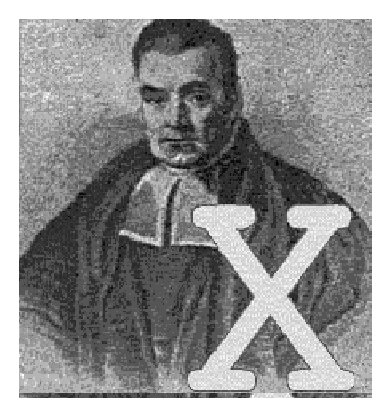
\includegraphics[scale=1.2]{grafiken/bayesicon.eps}
\end{center}
\end{figure}

\vfill

{\bf\sffamily \huge Methodology Manual}

\vfill

\end{center}

{\em Developed by}

Christiane Belitz \\
Andreas Brezger (HypoVereinsbank Munich) \\
Thomas Kneib (Ludwig-Maximilians-University Munich)\\
Stefan Lang (University of Innsbruck)\\

{\em With contributions by}


Eva-Maria Fronk\\
Andrea Hennerfeind\\
Manuela Hummel\\
Alexander Jerak\\
Petra Kragler\\
Leyre Osuna Echavarr\'{\i}a\\

{\em Supported by}

Ludwig Fahrmeir (mentally)\\
Leo Held (mentally)\\
German Science Foundation

\newpage

\subsection*{Acknowledgements}

The development of {\em BayesX} has been supported by grants from
the German National Science Foundation (DFG), Collaborative Research
Center 386 "Statistical Analysis of Discrete Structures".

Special thanks go to (in alphabetical order of first names):

{\em Achim Zeileis} for advertising HCL colors; \\
{\em Dieter Gollnow} for computing and providing the map of Munich (a really hard job); \\
{\em Leo Held} for advertising the program; \\
{\em Ludwig Fahrmeir} for his patience with finishing the program
and for carefully
reading and correcting the  manual; \\
{\em Ngianga-Bakwin Kandala} for being the first user of the program (a really hard job); \\
{\em Samson Babatunde Adebayo} for carefully reading and correcting the manual; \\
{\em Ursula Becker} for carefully reading and correcting the manual;

\subsection*{Licensing agreement} The authors of this software grant
to any individual or non-commercial organization the right to use
and to make an unlimited number of copies of this software. Usage by
commercial entities requires a license from the authors. You may not
decompile, disassemble, reverse engineer, or modify the software.
This includes, but is not limited to modifying/changing any icons,
menus, or displays associated with the software. This software
cannot be sold without written authorization from the authors. This
restriction is not intended to apply for connect time charges, or
flat rate connection/download fees for electronic bulletin board
services. The authors of this program accept no responsibility for
damages resulting from the use of this software and make no warranty
on representation, either express or implied, including but not
limited to, any implied warranty of merchantability or fitness for a
particular purpose. This software is provided as is, and you, its
user, assume all risks when using it.

\vspace{0.5cm}

{\em BayesX} is available at {
\href{http://www.stat.uni-muenchen.de/~bayesx}{http://www.stat.uni-muenchen.de/\~{}bayesx}}

\newpage

\section{Introduction}

In this manual we provide a brief overview of the methodological
background for the three regression tools currently implemented in
BayesX. The first regression tool ({\em bayesreg objects}) relies on
Markov chain Monte Carlo simulation techniques and yields fully
Bayesian posterior mean estimates. The second regression tool ({\em
remlreg objects}) is based on the mixed model representation of
penalised regression models with inference being based on penalised
maximum likelihood and marginal likelihood (a generalisation of
restricted maximum likelihood) estimation. The third regression tool
{\em stepwisereg objects} simultaneously  performs model choice and estimation.
Inference is based on a penalized likelihood point of view of STAR models. MCMC techniques are
partly used for computing interval estimates.
All regression tools
allow to estimate structured additive regression (STAR) models
(Fahrmeir, Kneib and Lang, 2004) with complex semiparametric
predictors. STAR models cover a number of well known model classes
as special cases, including {\em generalized additive models}
(Hastie and Tibshirani, 1990), {\em generalized additive mixed
models} (Lin and Zhang, 1999), {\em geoadditive models} (Kammann and
Wand, 2003), {\em varying coefficient models} (Hastie and
Tibshirani, 1993), and {\em geographically weighted regression}
(Fotheringham, Brunsdon, and Charlton, 2002). Besides models for
responses from univariate exponential families, BayesX also supports
non-standard regression situations such as models for categorical
responses with either ordered and unordered categories, continuous
time survival data, or continuous time multi-state models. To
provide a first impression of structured additive regression,
Sections~\ref{obsmodel} to \ref{inference} describe STAR models for
exponential family regression. Section~\ref{survivalAnalysis}
extends structured additive regression to the analysis of survival
times and multi-state data. Full details on STAR methodology can be
found in the following references:

\subsubsection*{Structured additive regression based on MCMC
simulation}

\begin{itemize}
\item Brezger, A., Lang, S. (2006)
      Generalized structured additive regression based on Bayesian P-Splines.
      Computational Statistics and Data Analysis, 50,
      967-991.\vspace{-0.25cm}
\item Fahrmeir, L., Lang, S. (2001)
      Bayesian Inference for Generalized Additive Mixed Models Based on Markov Random Field Priors.
      Journal of the Royal Statistical Society C (Applied Statistics), 50, 201-220.\vspace{-0.25cm}
\item Fahrmeir, L., Lang, S. (2001)
      Bayesian Semiparametric Regression Analysis of Multicategorical Time-Space Data.
      Annals of the Institute of Statistical Mathematics, 53, 10-30.\vspace{-0.25cm}
\item Fahrmeir, L., Osuna, L.. (2006)
      Structured additive regression for overdispersed and zero-inflated count data.
      Applied Stochastic Models in Business and Industry, 22, 351-369.\vspace{-0.25cm}
\item Hennerfeind, A., Brezger, A., Fahrmeir, L. (2006)
      Geoadditive survival models.
      Journal of the American Statistical Association, 101, 1065-1075.\vspace{-0.25cm}
\item Kneib, T., Hennerfeind, A. (2006)
      Bayesian Semiparametric Multi-State Models.
      SFB 386 Discussion Paper 502.\vspace{-0.25cm}
\item Lang, S., Brezger, A. (2004)
      Bayesian P-Splines
      Journal of Computational and Graphical Statistics, 13, 183-212.
\end{itemize}

Presumably the best starting point is the paper by Brezger and Lang (2006).

\subsubsection*{Structured additive regression based on mixed model
methodology}

\begin{itemize}
\item Fahrmeir, L., Kneib, T., Lang, S. (2004)
      Penalized structured additive regression for space-time data: a Bayesian perspective.
      Statistica Sinica, 14, 715-745.\vspace{-0.25cm}
\item Kneib, T. (2006):
      Mixed model based inference in structured additive regression.
      Dr. Hut Verlag, M\"{u}nchen.
      Available online from {\tt http://edoc.ub.uni-muenchen.de/archive/ 00005011/}\vspace{-0.25cm}
\item Kneib, T. (2006):
      Geoadditive hazard regression for interval censored survival times.
      Computational Statistics and Data Analysis, 51, 777-792.\vspace{-0.25cm}
\item Kneib, T., Fahrmeir, L. (2007):
      A mixed model approach for geoadditive hazard regression.
      Scandinavian Journal of Statistics, 34, 207-228.\vspace{-0.25cm}
\item Kneib, T., Fahrmeir, L. (2006):
      Structured additive regression for multicategorical space-time data: A mixed model approach.
      Biometrics, 62, 109-118.\vspace{-0.25cm}
\item Kneib, T., Hennerfeind, A. (2006)
      Bayesian Semiparametric Multi-State Models.
      Statistical Modeling, to appear.
\end{itemize}

Presumably the best starting point is the paper by Fahrmeir, Kneib and Lang (2004) or the monograph by Kneib (2006).

\subsubsection*{Structured additive regression including model selection}

\begin{itemize}
\item Belitz, C. (2007) Model selection in Generalised Structured Additive Regression Models. Dr. Hut Verlag, M\"{u}nchen.
\item Belitz, C.  and Lang, S. (2007) Simultaneous selection of variables and smoothing parameters
in structured additive regression models. Revised for Computational Statistics and Data Analysis.
\end{itemize}

Presumably the best starting point is the paper by Belitz and Lang (2007).

\subsubsection*{Guideline for the reader}


The rest of this manual is organized as follows:

The next section describes the general structure of STAR models for distributions
of the response variable belonging to an exponential family. The following
sections \ref{penalizedleastsquares} - \ref{inference}
discuss alternative approaches for specifying and estimating the different model terms
in STAR models.
Section \ref{penalizedleastsquares} describes the models from a more classical penalized
least squares respectively likelihood perspective. A Bayesian point of view is taken in
section \ref{priorassumptions}. The close connection to mixed models is highlighted in
section \ref{glmmrep}.
Section \ref{inference} gives a brief outline of the various inference techniques
for STAR models. Fully Bayesian inference via MCMC simulation techniques is the topic of subsection
\ref{fullbayes}. Inference based on mixed model technology is sketched in subsection  \ref{glmmmeth}.
Simultaneous selection of relevant model terms and estimation of the parameters is described in subsection
\ref{stepwiseest}.

For most users of BayesX it is sufficient to read only parts of this manual. Some recommendations
are given in the following Table \ref{guideline}.

\begin{table}[ht]
\footnotesize
\begin{center}
\begin{tabular}{|p{8cm}|p{5cm}|}
\hline
{\bf Intended use} & {\bf recommended sections } \\
\hline
semiparametric regression, fully Bayesian approach  & sections \ref{obsmodel}, \ref{priorassumptions} , \ref{fullbayes} \\
\hline
semiparametric regression, inference based on mixed model technology, classical perspective &
sections \ref{obsmodel}, \ref{penalizedleastsquares}, \ref{glmmrep}, \ref{glmmmeth} \\
\hline
semiparametric regression, inference based on mixed model technology, Bayesian point of view & sections \ref{obsmodel}, \ref{priorassumptions},
\ref{glmmrep}, \ref{glmmmeth} \\
\hline
semiparametric regression including model choice & sections \ref{obsmodel}, \ref{penalizedleastsquares}, \ref{stepwiseest} \\
\hline
\end{tabular}
{\em \caption {\label{guideline} Guidelines for reading this manual.}}
\end{center}
\end{table}


\section{Generalized regression models}
\label{obsmodel}

\index{Generalized linear model}\index{Exponential family}
Generalized linear models assume that, given covariates $\uvec$ and
unknown parameters $\gammavec$, the distribution of the response
variable $y$ belongs to an exponential family, i.e.
\begin{equation}
\label{likel} p(y \, | \, \uvec) = \exp \left( \frac{y \theta -
b(\theta)}{\phi} \right) c(y,\phi)
\end{equation}
where $b(\cdot)$, $c(\cdot)$, $\theta$ and $\phi$ determine the
specific response distribution. A list of the most common
distributions and their parameters can be found for example in
Fahrmeir and Tutz (2001), page 21. The mean $\mu=E(y|\uvec,\gammavec)$ is
linked to a linear predictor $\eta$ by
\begin{equation}
\label{glm} \mu=h(\eta) \qquad \eta= \uvec'\gammavec,
\end{equation}
where $h$ is a known response function and $\gammavec$ are unknown
regression parameters.

In most practical regression situations, however, we are facing at
least one of the following problems:
\begin{itemize}
\item For the {\em continuous covariates} in the data set, the assumption of a strictly linear
effect on the predictor may be not appropriate. \vspace{-0.2cm}
\item Observations may be {\em spatially correlated}.
\vspace{-0.2cm}
\item Observations may be {\em temporally correlated}.
\vspace{-0.2cm}
\item Complex interactions may be required to model the joint effect
of some of the covariates adequately. \vspace{-0.2cm}
\item  Heterogeneity among individuals or units may be not sufficiently described by covariates. Hence,
unobserved {\em unit or cluster specific heterogeneity} must be
considered appropriately.
\end{itemize}
To overcome these difficulties, we replace the strictly linear
predictor in (\ref{glm}) by a structured additive predictor
\begin{equation}
\label{gampred}
\eta=f_{1}(x_{1})+\ldots+f_{p}(x_{p})+\uvec'\gammavec,
\end{equation}
where $x_j$ denote
covariates of different type and dimension, and $f_j$ are (not
necessarily smooth) functions of the covariates. The functions $f_j$
comprise usual nonlinear effects of continuous covariates, time
trends and seasonal effects, two-dimensional surfaces, varying
coefficient models, i.i.d. random intercepts and slopes as well as
spatial effects. STAR-models cover a number of special cases
well known from the literature, in particular {\em Generalized additive models (GAM)},
{\em Generalized additive mixed models (GAM)}, {\em Geoadditive models}, {\em Multilevel models},
{\em Varying coefficient models (VCM)}, {\em ANOVA type interaction models} and {\em geographically weighted regression}.

%\begin{itemize}
%\item } \\
%A GAM is obtained if  the $x_j$, $j=1,\dots,p$, are univariate and
%continuous and $f_j$ are smooth functions.
%\index{Generalized additive model}
%\item {\em Generalized additive mixed model (GAMM)} \\
%A GAMM is included
%
%Consider longitudinal data for individuals $i=1,\dots,n,$ observed
%at time points $t \in \{ t_1,t_2,\dots \}$. For notational
%simplicity we assume the same time points for every individual,
%but generalizations to individual specific time points are
%obvious. A GAMM extends a GAM by introducing individual specific
%random effects, i.e.
%$$
%\eta_{it} = f_1(x_{it1})+\dots+f_k(x_{itk}) + b_{1i} w_{it1}  +
%\cdots + b_{qi} w_{itq}  + u_{it}'\gamma
%$$
%where $\eta_{it},x_{it1},\dots,x_{itk},w_{it1},\dots,w_{itq},u_{it}$
%are predictor and covariate values for individual $i$ at time $t$
%and $b_i=(b_{1i},\dots,b_{qi})$ is a vector of $q$ i.i.d.~random
%intercepts (if $w_{itj} = 1$) or random slopes. The random effects
%components are modelled by i.i.d.~Gaussian priors, see
%\autoref{random}. GAMM's can be subsumed into (\ref{gampred}) by
%defining $r=(i,t)$, $x_{rj} = x_{itj}$, $j=1,\dots,k$, $x_{r,k+h} =
%w_{ith}$, and $f_{k+h}(x_{r,k+h}) = b_{hi} w_{ith}$, $h=1,\dots,q$.
%Similarly, GAMM's for cluster data can be written in the general
%form (\ref{gampred}).\index{Generalized additive mixed model}
%
%\item {\em Geoadditive Models} \\
%In many situations additional geographic information is available
%for the observations in the data set. As an example, compare the
%demonstrating example on determinants of childhood undernutrition in
%Zambia in the tutorial manual. The district where the mother of a
%child lives is given as a covariate and may be used as an indicator
%for regional differences in the health status of children. A
%reasonable predictor for such data is given by
%\begin{equation}
%\eta_{r} = f_1(x_{r1})+\dots+f_k(x_{rk}) + f_{spat}(s_{r}) + u_r'
%\gamma
%\end{equation}
%where $f_{spat}$ is an additional spatially correlated effect of the
%location $s_{r}$ an observation pertains to. Models with a predictor
%that contains a spatial effect are also called geoadditive models,
%see Kammann and Wand (2003). In {\em BayesX}, spatial effects can be
%modeled by Markov random fields (Besag, York and Mollie (2003)),
%stationary Gaussian random fields (Kriging, Kamman and Wand, 2003),
%or two-dimensional P-splines (Lang and Brezger, 2006).\index{Geoadditive model}
%
%\item {\em Varying coefficient model (VCM) - Geographically weighted regression} \\
%A VCM as proposed by Hastie and Tibshirani (1993) is defined by
%$$
%\eta_{r} = g_1(w_{r1}) z_{r1} + \cdots + g_p(w_{rp}) z_{rp},
%$$
%where the effect modifiers $w_{rj}$ are continuous covariates or
%time scales and the interacting variables $z_{rj}$ are either
%continuous or categorical. A VCM can be cast into the general form
%(\ref{gampred}) with $x_{rj} = (w_{rj},z_{rj})$ and by defining the
%special function $f_j(x_{rj}) = f_j(w_{rj},z_{rj}) =
%g_j(w_{rj})z_{rj}$. Note that in {\em BayesX} the effect modifiers
%are not necessarily restricted to be continuous variables as in
%Hastie and Tibshirani (1993). For example, the geographical location
%may be used as effect modifier as well. VCMs with spatially varying
%regression coefficients are well known in the geography literature
%as {\em geographically weighted regression}, see e.g.~Fotheringham,
%Brunsdon, and Charlton (2002).\index{Varying coefficient
%models}\index{Geographically weighted regression}
%\item {\em ANOVA type interaction model} \\
%Suppose $w_{r}$ and $z_{r}$ are two continuous covariates. Then,
%the effect of $w_{r}$ and $z_{r}$ may be modelled by a predictor
%of the form
%$$
%\eta_r = f_{1}(w_{r})+f_{2}(z_{r})+f_{1|2}(w_{r},z_{r}) + \dots,
%$$
%see e.g. Chen (1993). The functions $f_1$ and $f_2$ are the main
%effects of the two covariates and $f_{1|2}$ is a two-dimensional
%interaction surface which can be modelled e.g. by two-dimensional
%P-splines, see \autoref{interactions}. The interaction can be cast
%into the form (\ref{gampred}) by defining $x_{r1}=w_r$, $x_{r2}=z_r$
%and  $x_{r3} = (w_{r},z_{r})$.
%\end{itemize}
%
%%At first sight it may look strange to use one general notation for
%%nonlinear functions of continuous covariates, i.i.d. random
%%intercepts and slopes, and spatially correlated effects as in
%%$(\ref{gampred})$. However, the unified treatment of the different
%%components in the model has several advantages:
%%\begin{itemize}
%%\item Since we adopt a Bayesian perspective it is generally not necessary to distinguish between
%%fixed and random effects because in a Bayesian approach all
%%unknown parameters are assumed to be random. \vspace{-0.2cm}
%%\item As we will see below in \autoref{priorassumptions}  the priors for smooth functions, two-dimensional
%%surfaces, i.i.d., serially and spatially correlated effects can be
%%cast into a general form as well. \vspace{-0.2cm}
%%\item The general form of both predictors and priors allows for rather general and unified estimation procedures,
%%see \autoref{inference}. As a  side effect the implementation and
%%description of these procedures is considerably facilitated.
%%\end{itemize}
%
\section{Penalized least squares and likelihood}
\label{penalizedleastsquares}

In BayesX the nonlinear functions $f_j$ are modeled by a basis functions approach, i.e. a particular nonlinear function $f$ is approximated by
a linear combination of basis functions:
$$
f(x) = \sum_{k=1}^{K} \beta_k B_k(x)
$$
The $B_k$ are known basis functions and $\betavec = (\beta_1,\dots,\beta_K)'$ is a vector of unknown regression coefficients to be estimated.
To ensure enough flexibility, typically a large number of basis functions is defined. To avoid overfitting a roughness penalty on the
regression coefficients
is additionally specified. We use quadratic penalties of the form $\betavec' \Pvec(\lambdavec) \betavec$ where $\Pvec(\lambdavec)$
is a penalty matrix. The penalty depends on one or multiple smoothing parameters $\lambdavec$ that govern the
amount of smoothness imposed on the function $f$. Most penalty matrices are of the particular simple form
$\Pvec(\lambdavec) = \lambda \Kvec$ where $\lambda$ is a scalar smoothing parameter. For {\em stepwisereg objects} more complicated
penalties are sometimes possible. They are an additive combination of penalty matrices. An example is
$\Pvec(\lambdavec) = \lambda_1 \Kvec_1+\lambda_2 \Kvec_2$ where $\lambda_1$ and $\lambda_2$ are smoothing parameters and $\Kvec_1$ and $\Kvec_2$
are penalty matrices.

The choice of basis functions $B_1,\dots,B_K$ and penalty  $\Pvec(\lambdavec)$ depends on our prior assumptions about the smoothness
of $f$ as well as
the type and dimension of $x$. We will give specific examples below. Defining the $n \times K$ design matrix $\Xvec$ with elements
$X[i,k] = B_k(x_i)$ the
vector $\fvec = (f(x_1),\dots,f(x_n))'$ of function evaluations can be written in matrix notation as $\fvec = \Xvec \betavec$.
Accordingly,  for model (\ref{gampred}) we obtain
$$
\etavec = \Xvec_1 \betavec_1 + \ldots + \Xvec_p \betavec_p + \Uvec \gammavec +  \varepsilonvec,
$$
where $\Uvec$ is the design matrix for linear effects, $\gammavec$ is the vector of regression coefficients for linear effects, and
$\varepsilonvec$
are the vectors of observations and errors.
In the next subsections we will give specific examples for modeling the unknown functions $f_j$ or in other words for the choice of basis functions and
penalty matrices.
We start with modeling the effect of continuous covariates using splines.

\subsection{Continuous covariates}
\subsubsection{P(enalized)-splines}
Suppose first that a particular component $x$ of the covariate  is univariate and continuous. There is a considerable
amount of literature on basis functions approaches
in combination with a (quadratic) roughness penalty for continuous covariates.
BayesX applies the P-splines approach introduced by Eilers and Marx (1996).
The approach assumes that the unknown functions can be approximated
by a polynomial spline of degree $l$
and with equally spaced knots
$$
x_{min} = \zeta_{0}  < \zeta_{1} < \dots < \zeta_{m-1} < \zeta_{m} = x_{max}
$$
over the domain of
$x$.
The spline can be written in terms of a linear combination of $K=m+l$
B-spline basis functions.
The columns of the design matrix $\Xvec$ are given by the B-spline basis functions
evaluated at the observations $x_i$. To overcome the well known difficulties involved with regression
splines, Eilers and Marx (1996)  suggest a relatively large
number of knots (usually between 20 to 40) to ensure enough
flexibility, and to introduce a roughness
penalty on adjacent regression coefficients based on
squared $r$-th order differences, i.e.
$$
\betavec' \lambda \Kvec \betavec = \lambda \sum_{k=r+1}^K (\Delta^r \beta_k)^2.
$$
The penalty matrix is given by $\Kvec =  \Dvec_r' \Dvec_r$ where $\Dvec_r$ is a $r$-th order difference matrix.
Typically, second or third order differences are used. The limiting behavior $\lambda \rightarrow \infty$ depends both on the
order of the spline
and the order of the penalty. If the order of the spline is equal to or
higher than the order of  the penalty, which is typically the case, then a polynomial
fit of degree $r-1$ is obtained in the limit.

The approach can be extended to impose monotonicity or more general shape constraints.
We follow an approach proposed by Bollaerts, Eilers, and Van Mechelen (2006).
A sufficient condition for a decreasing
spline is given by $\beta_{k} \leq \beta_{k-1}$, i.e.  a parameter $\beta_{k}$ is less than its predecessor $\beta_{k-1}$.
The simple but powerful idea  is to impose the
required constraint by expanding the penalty by an additional  term. More specifically they propose
the composed penalty
$$
\Pvec(\lambdavec) =  \betavec' \left( \lambda_1 \Kvec_1 + \lambda_2 \Kvec_2 \right) \betavec
$$
where $\lambda_1$ and $\Kvec_1$ are the usual smoothing parameter and penalty matrix for P-splines.
The additional penalty matrix $\Kvec_2$ is a diagonal matrix with entries 1 whenever the
condition $\beta_{k} \leq \beta_{k-1}$ fails and 0 otherwise.
For increasing functions $\Kvec_2$ has to be adapted accordingly. The parameter $\lambda_2$ is not estimated but set large enough to
produce monotonic functions.





\subsubsection{Tensor product P-splines}
\label{tensorproductpsplines}
Assume now that $x$ is two dimensional, i.e.
$x = \left(x^{(1)},x^{(2)}\right)'$ with continuous components
$x^{(1)}$ and $x^{(2)}$. The aim is to extend the univariate
P-spline from the preceding section to two dimensions.
A common approach is to approximate the unknown surface $f(x)$ by the tensor product of one
dimensional B-splines, i.e.
\begin{equation}
\label{gampspline_2dimterm} f\left(x^{(1)},x^{(2)}\right) = \sum_{k=1}^{K_1}
\sum_{s=1}^{K_2} \beta_{ks} B_{1,k}(x^{(1)})
B_{2,s} (x^{(2)}),
\end{equation}
where $B_{11},\dots,B_{1K_1}$ are the basis functions in $x^{(1)}$ direction and
$B_{21},\dots,B_{2K_2}$ in $x^{(2)}$ direction.
The $n \times K = n \times K_1 K_2$ design matrix $\Xvec$ now consists of
products of basis functions.

Several alternatives are available for the penalty matrix $\Pvec(\lambdavec)$:
\begin{enumerate}
\item[a)] {\em Penalty based on first differences:} The
two dimensional generalization of a penalty based on first differences is given by combining row- and column wise quadratic differences
$$
\begin{array}{l}
\displaystyle \sum_{k=2}^{K_1}\sum_{s=1}^{K_2}(\beta_{ks}-\beta_{k-1,s})^2 =
\betavec'(\Ivec_{K_2}\otimes \Dvec_1)'(\Ivec_{K_2}\otimes \Dvec_1)\betavec \\[0.4cm]
\displaystyle  \sum_{k=1}^{K_1}\sum_{s=2}^{K_2}(\beta_{ks}-\beta_{k,s-1})^2 =
\betavec'(\Dvec_2\otimes \Ivec_{K_1})'(\Dvec_2\otimes \Ivec_{K_1})\betavec \\
\end{array}
$$
to the penalty
$$
\betavec'\Pvec(\lambdavec) \betavec =  \betavec' \lambda \left[ (\Ivec_{K_2}\otimes \Dvec_1)'(\Ivec_{K_2}\otimes \Dvec_1) + (\Dvec_2\otimes \Ivec_{K_1})'
(\Dvec_2\otimes \Ivec_{K_1})\right]\betavec.
$$
Another way of expressing the penalty is given by
\begin{equation}
\label{2dpenalty}
 \betavec'\Pvec(\lambda)\betavec = \betavec'\lambda \left[\Ivec_{K_2}\otimes\Kvec_1 + \Kvec_2\otimes \Ivec_{K_1}\right]\betavec,
\end{equation}
where $\Kvec_1$ and $\Kvec_2$ are the respective one dimensional penalty matrices.
In the limit  $\lambda \rightarrow \infty$ a constant fit is obtained.
\item[b)] {\em Penalty based on second differences:} In a similar way two dimensional penalties based on higher order differences
are constructed. A second order difference penalty is obtained if  $\Kvec_1$ and $\Kvec_2$ in (\ref{2dpenalty}) correspond to
penalty matrices based on second rather than first differences.
Similar to one dimensional P-splines the limit $\lambda \rightarrow \infty$ results in a linear fit, i.e.
$$
f\left(z^{(1)},z^{(2)}\right) = c_0 + c_1 \, z^{(1)} + c_2 \, z^{(2)} + c_3 \, z^{(1)} z^{(2)}.
$$
\item[c)] {\em Anisotropic penalty:} The two penalties considered so far are not capable of
different penalization in $z^{(1)}$ and $z^{(2)}$ direction, respectively. Anisotropic penalties are obtained by assuming
separate smoothing parameters $\lambda_1$ and $\lambda_2$ in $z^{(1)}$ and $z^{(2)}$ direction. The penalty is then given by
\begin{equation}
\label{penalty_eilmar}
 \betavec'\Pvec(\lambdavec) \betavec = \betavec'\left[\lambda_1 \Ivec_{K_2}\otimes\Kvec_1 + \lambda_2 \Kvec_2\otimes \Ivec_{K_1}\right]\betavec.
\end{equation}
The resulting fit in the limit $\lambda_1 \rightarrow \infty$ and $\lambda_2 \rightarrow \infty$ depends on the penalty used to construct
$\Kvec_1$ and $\Kvec_2$. If $\Kvec_1$ and $\Kvec_2$ correspond to a first order difference penalty a constant fit is obtained in the limit.
Second order difference penalties result in a linear fit for $f\left(z^{(1)},z^{(2)}\right)$.
\item[d)] {\em Penalties with main effects in the limit:} Sometimes it is desirable to decompose the effect of the two covariates
$z^{(1)}$ and $z^{(2)}$ into two main effects modeled by one dimensional functions
and a two dimensional interaction effect, i.e.
\begin{equation}
\label{gampspline_2dimtermmain}
f \left(z^{(1)},z^{(2)}\right) = f_1\left(z^{(1)} \right) +
f_2 \left(z^{(2)}\right) + f_{1|2}\left( z^{(1)},z^{(2)} \right).
\end{equation}
Usually a two dimensional surface smoother  together with two additional  one dimensional P-splines
(or other smoothers) are estimated. This approach is possible with {\em bayesreg objects} and {\em remlreg objects}.
{\em stepwisereg objects} take, however, a different approach. We specify a two dimensional surface based on tensor product P-splines and
compute the decomposition of the
resulting surface
into main effects and the interaction effect {\em after} estimation. Moreover, we specify a penalty that allows for a main effects only
model as a special
case. This allows to discriminate between a simple  main effects model and a more complicated two way interactions model.
A penalty that guarantees  a main effects model in the limit is defined by the Kronecker product of the two penalty matrices for one dimensional P-splines, i.e.
\begin{equation}
\label{penalty_kronecker}
\betavec'\Pvec(\lambda)\betavec = \betavec' \lambda \Kvec_1 \otimes \Kvec_2 \betavec.
\end{equation}
The drawback of this penalty is that the limit $\lambda \rightarrow \infty $ yields {\em unpenalized} main effects, i.e. wiggly functions.
We therefore use a modified penalty which is effectively a combination of the two  penalties  (\ref{penalty_eilmar}) and
(\ref{penalty_kronecker}). More specifically
we define
\begin{equation}
\label{penalty_comb}
\betavec'\Pvec(\lambdavec)\betavec = \betavec' \left[\frac{\lambda_1}{K_1}
\Ivec_{K_2}\otimes\Kvec_1 + \frac{\lambda_2}{K_2} \Kvec_2\otimes \Ivec_{K_1}+\lambda_3 \Kvec_1 \otimes \Kvec_2   \right] \betavec,
\end{equation}
where $\Kvec_1$ and $\Kvec_2$ are penalty matrices corresponding to one dimensional P-splines based on first or second order differences.
This penalty has the following nice properties:
\begin{itemize}
\item The limit $\lambda_3 \rightarrow \infty$ results in a mere main effects model. The main effects  are one dimensional P-splines with smoothing
parameters $\lambda_1$ and $\lambda_2$.
\item The limit $\lambda_3 \rightarrow 0$ yields the anisotropic penalty (\ref{penalty_eilmar}) as a special case.
\item The limit $\lambda_1 \rightarrow 0$ and $\lambda_2 \rightarrow 0$  yields the Kronecker product penalty
(\ref{penalty_kronecker}) as a special case.
\item The limit $\lambda_1 \rightarrow \infty$, $\lambda_2 \rightarrow \infty$ and $\lambda_3 \rightarrow \infty$ results in a main effects model with
linear or constant main effects depending on the difference order used to construct $\Kvec_1$ and $\Kvec_2$.
\end{itemize}
\end{enumerate}





\subsection{Spatial heterogeneity}
In this subsection we assume that $x$ represents the location a particular observation pertains to.
The location is typically given in two ways. If exact locations
are available $x=(x^{(1)},x^{(2)})'$ is two dimensional and the components  $x^{(1)}$ and $x^{(2)}$ correspond to the coordinates of the location.
In this case the spatial effect $f(x^{(1)},x^{(2)})$ could be modeled by
two dimensional surface estimators as described in the preceding section.

In many applications, however, exact locations are not available. Typically, a geographical map is available and $x \in \{1,\dots,K\}$ is an
index that denotes the region (e.g. district) an observation pertains to. A common approach is to assume $f(x) = \beta_x$,
i.e. separate parameters $\beta_1,\ldots,\beta_K$  for each region are estimated.
The $n \times K$ design matrix $\Xvec$ is an incidence matrix whose entry in
the $i$-th row and $k$-th column is equal to one if observation $i$ has been observed at
location $k$ and zero otherwise. To prevent overfitting a penalty based on squared differences is defined that
guarantees that parameters of neighboring regions are similar. Typically two regions are assumed to be neighbors if they share a common
boundary although other neighborhood definitions are possible. The penalty is defined as
$$
\betavec' \lambda \Kvec \betavec = \lambda\sum_{k=2}^{K}\sum_{s \in N(k), s < k}(\beta_k-\beta_s)^2,
$$
where $N(k)$ denotes all sites that are neighbors of site $k$.
The elements of the penalty matrix are given by
\begin{equation}
\label{K_mrf}
 \Kvec[s,r] = \lambda \left\{
 \begin{array}{ll}
-1 & k\neq s, k\sim s,\\
 0 & k\neq s, k \nsim s,\\
 |N(k)| & k=s.
\end{array}
\right.
\end{equation}

Depending on the prior belief on smoothness of the spatial effect several alternatives to penalty (\ref{K_mrf}) are available.
If a very smooth effect is assumed the two dimensional smoothers discussed in the preceding section could be used as an alternative.
Since exact locations are not available the centroids of the regions could be used instead.
In some situations a smooth spatial effect is not justified because of local, spatial heterogeneity. In this case,
the assumption of spatial dependence of neighboring parameters is not meaningful. Instead, a simple ridge type penalty
$$
\betavec' \lambda \Kvec \betavec = \lambda \betavec'  \betavec = \lambda \sum_{k=1}^{K} \beta_k^2
$$
with penalty matrix $\Kvec = \Ivec$ may be defined. This penalty does not assume any spatial dependence but prevents highly variable
estimates induced by small samples for some regions or sites.

\subsection{Unit- or cluster specific heterogeneity}
Typically, unit- or cluster specific random effects are introduced to account
for heterogeneity. In its simplest form a random intercept $\beta_x$ with $\beta_x \sim N(0,\tau^2)$ is introduced.
Here, $x \in \{1,\dots,K\}$ is an index variable that denotes the cluster a particular observation pertains to.
This is equivalent to a penalized least squares approach with function $f(x) = \beta_x$, penalty matrix $\Ivec$ and smoothing parameter
$\lambda = \sigma^2/\tau^2$. The $n \times K$ design matrix $\Xvec$ is a 0/1 incidence matrix whose entry in
the $i$-th row and $k$-th column is equal to one if observation $i$ belongs to the $k$-th cluster and zero otherwise.
Random slopes could be treated in the same way, see the next subsection.

Note that more than one random intercept with respect to different cluster variables are possible. In many cases there exists a hierarchical ordering
of clusters. Models with such hierarchical clusters are also called multilevel models.


\subsection{Varying coefficients}
\label{varcoeff_terms}

Suppose now that the effect of a continuous covariate $x^{(2)}$ is assumed to vary with
respect to a categorical covariate $x^{(1)}$. For notational convenience, we restrict the discussion to binary covariates $x^{(1)}$.
The generalization to (multi)categorical covariates is straightforward.
The interaction between $x^{(2)}$ and
$x^{(1)}$ can be modeled by a predictor of the form
$$
\eta = \ldots + f_1(x^{(2)}) + g(x^{(2)}) x^{(1)} + \ldots,
$$
where $f_1$ and $g$ are smooth functions (modeled by P-splines).
The interpretation of the two functions $f_1$ and $g$ depends on the coding of the binary variable $x^{(1)}$.
If $x^{(1)}$ is in dummy-coding, the function $f_1$ corresponds to the effect of $x^{(2)}$ subject to  $x^{(1)}=0$, and
$g$ is the difference effect for observations with $x^{(1)}=1$. If $x^{(1)}$ is in effect-coding, the function $f_1$ can be interpreted as an
average effect of  $x^{(2)}$, and $g$ respectively $-g$ is now the deviation from $f_1$ for $x^{(1)} = 1$ and $x^{(1)} = -1$, respectively.
It turns out that the coding of $x^{(2)}$ is not only important  for interpretation but sometimes also crucial for inference
(in {\em bayesreg objects} and {\em remlreg objects}). Estimation for {\em bayesreg and stepwisereg objects} described
in the next section is based on an iterative backfitting type procedure. Hence dependence between $f_1$ and $g$ should be minimized to avoid
convergence problems. Hence, effect coding for $x^{(2)}$ is an effective yet simple device to avoid convergence problems.

Models with interaction effects of the form $g(x^{(2)}) \, x^{(1)}$ are  known as varying coefficient models  because
the effect of $x^{(1)}$ varies smoothly with respect to the continuous covariate $x^{(2)}$. Covariate $x^{(2)}$ is called the effect modifier of
$x^{(1)}$. The approach can be easily extended to a two dimensional effect modifier with components $x^{(2)}$ and $x^{(3)}$.
The interaction effect is then given by $g(x^{(2)},x^{(3)}) \, x^{(1)}$ where $g(x^{(2)},x^{(3)})$ is a two dimensional surface which is  modeled
by the tensor product P-splines discussed in section \ref{tensorproductpsplines}.
Another modification arises if the
effect modifier is the location either given as the coordinates or as a spatial index. In this case we have a space varying effect of $x^{(1)}$.
Models of this kind are also known as geographically weighted regression, see Fotheringham, Brunsdon and Charlton (2002).
A final modification is obtained for a unit- or
cluster index as the effect modifier. The effect of $x^{(1)}$ is now assumed to be unit- or cluster specific and typically referred to as a random slope.

Independent of the specific type of the effect modifier, the interaction term $g\left(x^{(2)}\right) \, x^{(1)}$
(or $g\left(x^{(2)},x^{(3)}\right) \, x^{(1)}$) can be cast into our
general framework by defining
\begin{equation}
\label{gampspline_varcoeffterm}
f\left(x^{(1)},x^{(2)}\right) = g\left(x^{(2)}\right) \, x^{(1)} \quad \mbox{or} \quad  f\left(x^{(1)},x^{(2)},x^{(3)}\right) =
g\left(x^{(2)},x^{(3)}\right) \, x^{(1)}.
\end{equation}
The overall design matrix $\Xvec$ is given by
$diag(x_{1}^{(1)},\dots,x_{n}^{(1)}) \, \Xvec^{(1)}$ where
$\Xvec^{(1)}$ is the usual design matrix for P-Splines,
tensor product P-splines, spatial- or cluster specific effects.



\section{Bayesian point of view}
\label{priorassumptions}\index{Prior assumptions}

For Bayesian inference, the unknown functions $f_{1},\dots ,f_{p}$
in predictor (\ref{gampred}), more exactly corresponding vectors of
function evaluations, and the fixed effects parameters $\gammavec$ are
considered as random variables and must be supplemented by
appropriate prior assumptions.

In the absence of any prior knowledge, diffuse priors are the
appropriate choice for fixed effects parameters, i.e.
$$
 p(\gamma_j) \propto const
$$
Another common choice, not yet supported by {\em BayesX}, are
informative multivariate Gaussian priors with mean $\muvec_0$ and
covariance matrix $\Sigmavec_0$.\index{Prior assumptions!Fixed effects}


Priors for the unknown functions $f_{1},\dots,f_{p}$ depend on the
{\em type of the covariates} and on {\em prior beliefs about the
smoothness of $f_j$.} In the following we express the vector of
function evaluations $\fvec_j=(f_j(x_{1j}),\dots,f_j(x_{nj}))'$ of a
function $f_j$ as the matrix product of a design matrix $\Xvec_j$ and a
vector of unknown parameters $\betavec_j$, i.e.
\begin{equation}
\label{matproduct} \fvec_j=\Xvec_j \betavec_j.
\end{equation}
Then, we obtain the predictor (\ref{gampred}) in matrix notation
as
\begin{equation}
\label{gampredmatrix} \etavec = \Xvec_1 \betavec_1 + \cdots + \Xvec_p \betavec_p +
\Uvec \gammavec,
\end{equation}
where $\Uvec$ corresponds to the usual design matrix for fixed
effects.

A prior for a function $f_j$ is defined by specifying a suitable
design matrix $\Xvec_j$ and a prior distribution for the vector
$\betavec_j$ of unknown parameters. The general form of the prior for
$\betavec_j$ is given by
\begin{equation}
\label{genform} p(\betavec_j | \tau_j^2) \propto
\frac{1}{(\tau^2_j)^{rank(\Kvec_j)/2}} \exp\left(-\frac{1}{2\tau_j^2}
\betavec_j' \Kvec_j \betavec_j\right),
\end{equation}
where $\Kvec_j$ is a {\em penalty matrix}. In most cases $\Kvec_j$ will be
rank deficient and therefore the prior for $\betavec_j$ is partially improper.

The variance parameter $\tau_j^2$ is  equivalent to the inverse
smoothing parameter in a penalized likelihood approach and controls the
trade off between flexibility and smoothness.

In the following we will describe specific priors for different
types of covariates and functions $f_j$.


\subsection{Priors for continuous covariates and time scales}
\label{psplines}\index{Continuous covariates}\index{Time scales}
\index{Prior assumptions!Continuous covariates}

Several alternatives have been  proposed for specifying smoothness
priors for continuous covariates or time scales. These are {\em
random walk priors} or more generally {\em autoregressive priors}
(see Fahrmeir and Lang, 2001a, and Fahrmeir and Lang, 2001b), {\em
Bayesian P-splines} (Lang and Brezger, 2006) and {\em Bayesian
smoothing splines} (Hastie and Tibshirani, 2000). {\em BayesX}
supports random walk priors and P-splines.

\subsubsection{Random walks}\index{Random walk priors}

Suppose first that $x$ is a time scale or continuous covariate
with equally spaced ordered observations
$$
x^{(1)} < x^{(2)} < \cdots < x^{(K)}.
$$
Here $K \leq n$ denotes the number of {\em different} observed
values for $x$ in the data set. A common approach in dynamic or
state space models is to estimate one parameter $\beta_{k}$ for
each distinct $x^{(k)}$, i.e. $f(x^{(k)}) = \beta_{k}$, and
penalize too abrupt jumps between successive parameters using random
walk priors. For example, first and second order random walk models
are given by
\begin{equation}
\label{rwpriors}
\beta_{k}=\beta_{k-1}+u_{k}\,\,\,\,\mbox{and}\,\,\,\,\beta_{k}=2\beta_{k-1}-\beta_{k-2}+u_{k}
\end{equation}
with Gaussian errors $u_{k}\sim N(0,\tau^{2})$ and diffuse priors
$p(\beta_{1})\propto const$, and $p(\beta_{1})$ and
$p(\beta_{2})\propto const$, for initial values, respectively. Both
specifications act as smoothness priors that penalize too rough
functions $f$. A first order random walk penalizes abrupt jumps
$\beta_{k}-\beta_{k-1}$ between successive states while a second
order random walk penalizes deviations from the linear trend $2
\beta_{k-1}-\beta_{k-2}$. The joint distribution of the
regression parameters $\betavec$ is easily computed as the product of
conditional densities defined by (\ref{rwpriors}) and can be brought
into the general form (\ref{genform}). The penalty matrix is of the
form $\Kvec=\Dvec'\Dvec$ where $\Dvec$ is a first or second order difference
matrix. For example, for a random walk of first order the penalty
matrix is given by:
$$
\Kvec = {\footnotesize \left(
\begin{array}{rrrrr}
 1 & -1 & & &  \\
-1 & 2 & -1 & & \\
 &  \ddots & \ddots & \ddots &  \\
 & & -1 & 2 & -1 \\
  & & & -1 & 1
\end{array}
\right) }.
$$
The design matrix $\Xvec$ is a simple 0/1 matrix where the number of
columns equals the number of parameters, i.e. the number of distinct
covariate values. If for the $i$-th observation $x_{i}=x^{(k)}$
the element in the $i$-th row and $k$-th column of $\Xvec$ is one and
zero otherwise.

In case of non-equally spaced observations slight modifications of
the priors defined in (\ref{rwpriors}) are necessary, see Fahrmeir
and Lang (2001a) for details.

If $x$ is a time  scale we may introduce an additional seasonal
effect of $x$. A common smoothness prior for a seasonal
component $f(x^{(k)}) = \beta_{k}$ is given by
\begin{equation}
\beta_{k} = -\beta_{k-1} - \cdots -
\beta_{k-per-1}+u_{k}\label{seasonal}
\end{equation}
where $u_{k} \sim N(0,\tau_j^{2})$ and $per$ is the period of the
seasonal effect (e.g. $per = 12$ for monthly data). Compared to a
dummy variable approach this specification has the advantage that it
allows for a time varying rather than a time constant seasonal
effect.


\subsubsection{P-splines}\index{P-splines}

A second approach for effects of continuous covariates, that is
closely related to random walk models, is based on P-splines
introduced by Eilers and Marx (1996). The approach assumes that an
unknown smooth function $f$ of a covariate $x$ can be
approximated by a polynomial spline of degree $l$ defined by a set
of equally spaced knots $x^{min} = \zeta_{0}  < \zeta_{1} < \dots
< \zeta_{m-1} < \zeta_{m} = x^{max}$ within the domain of $x$.
Such a spline can be written in terms of a linear combination of
$K = m+l$ B-spline basis functions $B_{k}$, i.e.
$$
f(x) = \sum_{k=1}^{K} \beta_{k} B_{k}(x).
$$
In this case, $\betavec = (\beta_{1},\dots,\beta_{K})'$
corresponds to the vector of unknown regression coefficients and the
$n \times K$ design matrix $\Xvec$ consists of the basis functions
evaluated at the observations $x_{i}$, i.e. $\Xvec[i,k] =
B_k(x_{i})$. The crucial point is the choice of the number of
knots. For a small number of knots, the resulting spline may not be
flexible enough to capture the variability of the data. For a large
number of knots, estimated curves tend to overfit the data and, as a
result, too rough functions are obtained. As a remedy, Eilers and
Marx (1996) suggest a moderately large number of equally spaced
knots (usually between 20 and 40) to ensure enough flexibility, and
to define a roughness penalty based on first or second order
differences of adjacent B-Spline coefficients to guarantee
sufficient smoothness of the fitted curves. This leads to penalized
likelihood estimation with penalty terms
\begin{equation}
\label{diffpenalty} \lambda \sum_{k=r+1}^{K}
(\Delta^r \beta_{k})^2 , \quad r=1,2
\end{equation}
where $\lambda$ is the smoothing parameter. First order
differences penalize abrupt jumps $\beta_{k}-\beta_{k-1}$ between
successive parameters while second order differences penalize
deviations from the linear trend $2 \beta_{k-1}-\beta_{k-2}$. In
a Bayesian approach we use the stochastic analogue of difference
penalties, i.e. first or second order random walks, as priors for
the regression coefficients. Note that simple first or second order
random walks can be regarded as P-splines of degree $l=0$ and are
therefore included as a special case. More details about Bayesian
P-splines can be found in Lang and Brezger (2004) and Brezger and
Lang (2006).


\subsection{Priors for spatial effects}\index{Spatial
priors}\index{Markov random fields}\index{Kriging}\index{Gaussian
random fields} \label{spatial}\index{Prior assumptions!Spatial
effects}

Suppose that the index $s \in \{ 1,\dots,S \}$ represents the
location or site in connected geographical regions. For simplicity
we assume that the regions are labelled consecutively. A common way
to introduce a spatially correlated effect is to assume that
neighboring sites are more alike than arbitrary sites. Thus, for a
valid prior definition a set of neighbors for each site $s$ must be
defined. For geographical data one usually assumes that two sites
$s$ and $s'$ are neighbors if they share a common boundary.

The simplest (but most frequently used) spatial smoothness prior for
the function evaluations $f(s)=\beta_{s}$ is given by
\begin{equation}
\label{adjacency} \beta_{s} | \beta_{s'}, \, {s \neq
s'},\tau^2 \sim N \left( \frac{1}{N_s} \sum_{s' \in \partial_s}
\beta_{s'} , \frac{\tau^2}{N_s} \right),
\end{equation}
where $N_s$ is the number of adjacent sites and $s' \in
\partial_s$ denotes that site $s'$ is a neighbor of site $s$. Hence,
the (conditional) mean of $\beta_{s}$ is an unweighted average of
function evaluations of neighboring sites. The prior is a direct
generalization of a first order random walk to two-dimensions and is
called a Markov random field (MRF).

A more general prior including (\ref{adjacency}) as a special case
is given by
\begin{equation}
\label{intrinsic} \beta_{s} | \beta_{s'} \, \, {s \neq
s'},\tau^2 \sim N \left( \sum_{s' \in \partial_s}
\frac{w_{ss'}}{w_{s+}} \beta_{s'}, \frac{\tau^2}{w_{s+}} \right),
\end{equation}
where $w_{ss'}$ are known weights and $+$ denotes summation over the
missing subscript. Such a prior is called a Gaussian intrinsic
autoregression, see Besag, York and Mollie (1991) and Besag and
Kooperberg (1995). Other weights than $w_{ss'} = 1$ as in
(\ref{adjacency}) are based on the common boundary length of
neighboring sites, or on the distance of the centroids of two sites.
All these spatial priors are supported by {\em BayesX}, see chapter
\ref*{map} of the reference manual for more details.

The $n \times S$ design matrix $\Xvec$ is a 0/1 incidence matrix. Its
value in the $i$-th row and the $s$-th column is 1 if the $i$-th
observation is located in site or region $s$, and zero otherwise.
The $S \times S$ penalty matrix $\Kvec$ has the form of an adjacency
matrix.

If exact locations $s=(s_x,s_y)$ are available, we can use
two-dimensional surface estimators to model spatial effects. One
option are two-dimensional P-splines, see \autoref{interactions}.
Another option are Gaussian random field (GRF) priors, originating
from geostatistics. These can also be interpreted as two-dimensional
surface smoothers based on radial basis functions and have been
employed by Kammann and Wand (2003) to model the spatial component
in Gaussian regression models. The spatial component
$f(s)=\beta_s$ is assumed to follow a zero mean stationary
Gaussian random field $\{\beta_s:s\in\mathbb{R}^2\}$ with variance
$\tau^2$ and isotropic correlation function
$cov(\beta_s,\beta_{s+h})=C(||h||)$. This means that correlations
between sites that are $||h||$ units apart are the same, regardless
of direction and the sites location. For a finite array
$s\in\{1,\ldots,S\}$ of sites as in image analysis, the prior for
$\betavec=(\beta_1,\ldots,\beta_S)'$ is of the general form
(\ref{genform}) with $\Kvec=\Cvec^{-1}$ and
\[\Cvec(i,j)=C(||s_i-s_j||), 1\le i,j\le S.\]
The design matrix $X$ is again a 0/1 incidence matrix.

Several proposals for the choice of the correlation function
$C(r)$ have been made. In the kriging literature, the Mat\'{e}rn
family $C(r;\rho,\nu)$ is highly recommended. For prechosen values $\nu=m+1/2$,
$m=0,1,2,\ldots$ of the smoothness parameter $\nu$ simple
correlation functions $C(r;\rho)$ are obtained, e.g.
\[C(r;\rho)=\exp(-|r/\rho|)(1+|r/\rho|)\]
with $\nu=1.5$. The parameter $\rho$ controls how fast correlations
die out with increasing $r=||h||$. It can be determined in a
preprocessing step or may be estimated jointly with the variance
components by restricted maximum likelihood. A simple rule, that
also ensures scale invariance of the estimates, is to choose $\rho$
as
\[\hat{\rho}=\max_{i,j}||s_i-s_j||/c.\]
The constant $c>0$ is chosen in such a way, that $C(c)$ is small,
e.g. 0.001. Therefore the different values of
$||s_i-s_j||/\hat{\rho}$ are spread out over the $r$-axis of the
correlation function. This choice of $\rho$ has proved to work well
in our experience.

Although we described them separately, approaches for exact
locations can also be used in the case of connected geographical
regions, e.g. based on the centroids of the regions. Conversely, we
can also apply MRFs to exact locations if neighborhoods are defined
based on a distance measure. In general, it is not clear which of
the different approaches leads to the ''best'' fits. For data
observed on a discrete lattice MRFs seem to be most appropriate. If
the exact locations are available, surface estimators may be more
natural, particularly because predictions for unobserved locations
are available. However, in some situations surface estimators lead
to an improved fit compared to MRF's even for discrete lattices and
vice versa. A general approach that can handle both situations is
given by M\"{u}ller et al. (1997).

From a computational point of view MRF's and P-splines are
preferable to GRF's because their posterior precision matrices are
band matrices or can be transformed into a band matrix like
structure. This special structure considerably speeds up
computations, at least for inference based on MCMC techniques. For
inference based on mixed models, the main difference between GRFs
and MRFs, considering their numerical properties, is the dimension
of the penalty matrix. For MRFs the dimension of $K$ equals the
number of different regions $S$ and is therefore independent from
the sample size. On the other side, for GRFs, the dimension of $K$
is given by the number of distinct locations, which is usually close
to the sample size. Therefore, the number of regression coefficients
used to describe a MRF is usually much smaller than for a GRF and
therefore the estimation of GRFs is computationally much more
expensive. To overcome this difficulty Kammann and Wand (2003)
propose low-rank kriging to approximate stationary Gaussian random
fields. Note first, that we can define GRFs equivalently based on a
design matrix $\Xvec$ with entries $\Xvec[i,j]=C(||s_i-s_j||)$ and penalty
matrix $\Kvec=\Cvec$. To reduce the dimensionality of the estimation problem
we define a subset of knots
$\mathcal{D}=\{\kappa_1,\ldots,\kappa_M\}$ of the set of distinct
locations $\mathcal{C}$. These knots can be chosen to be
''representative'' for the set of distinct locations $\mathcal{C}$
based on a space filling algorithm. Therefore consider the distance
measure
\[d(s,\mathcal{D})=\left(\sum_{\kappa\in\mathcal{D}}||s-\kappa||^p\right)^{\frac{1}{p}},\]
with $p<0$, between any location $s\in\mathcal{D}$ and a possible
set of knots $\mathcal{C}$. Obviously this distance measure is
zero for all knots. Using a simple swapping algorithm to minimize
the overall coverage criterion
\[\left(\sum_{s\in\mathcal{C}}d(s,\mathcal{D})^q\right)^{\frac{1}{q}}\]
with $q>0$ (compare Johnson et al. (1990) and Nychka and Saltzman
(1998) for details) yields an optimal set of knots $\mathcal{D}$.
Based on these knots we define the approximation $f=\Xvec\betavec$
with the $n\times M$ design matrix $X[i,j]=C(||s_i-\kappa_j||)$,
penalty matrix $\Kvec=\Cvec$, and $\Cvec[i,j]=C(||\kappa_i-\kappa_j||)$. The
number of knots $M$ allows to control the trade-off between accuracy
of the approximation ($M$ close to the sample size) and numerical
simplification ($M$ small).

\subsection{Unordered group indicators and unstructured spatial effects}
\label{random}\index{Random effects}\index{Group
indicators}\index{Unstructured spatial effects}

In many situations we observe the problem of heterogeneity among
clusters of observations caused by unobserved covariates. Neglecting
unobserved heterogeneity may lead to considerably biased estimates
for the remaining effects as well as false standard error estimates.
Suppose now $x \in \{1,\dots,K\}$ is a cluster variable indicating the
cluster a particular observation belongs to. A common approach to
overcome the difficulties of unobserved heterogeneity is to
introduce additional Gaussian i.i.d. effects $f(x) = \beta_{x}$
with
\begin{equation}
\label{randomeff} \beta_{x} \sim N(0,\tau^2), \quad
x=1,\dots,K.
\end{equation}
The design matrix $\Xvec$ is again a $n \times K$-dimensional 0/1
incidence matrix that represents the grouping structure of the data,
while the penalty matrix is simply the identity matrix, i.e.
$\Kvec=\Ivec$. From a classical perspective, (\ref{randomeff}) defines
i.i.d. {\em random effects}. However, from a Bayesian point of view
all unknown parameters are assumed to be random and hence the
notation "random effects" in this context is misleading. Hence, one
may also think of (\ref{randomeff}) as an approach for modelling an
unsmooth function.

Prior (\ref{randomeff}) may also be used for a more sophisticated
modelling of spatial effects. In some situation it may be useful to
split up the spatial effect $f_{spat}$ into a spatially correlated
(structured) part $f_{str}$ and a spatially uncorrelated
(unstructured) part $f_{unstr}$, i.e.
$$
f_{spat} = f_{str}+f_{unstr}.
$$
A rationale is that a spatial effect is usually a surrogate of many
unobserved influential factors, some of which obeying a strong
spatial structure while others are present only locally. By
estimating a structured and an unstructured component we aim at
distinguishing between the two kinds of influential factors, see
also Besag, York and Mollie (1991). For the smooth spatial part we
can assume any of the spatial priors discussed in \autoref{spatial}.
For the uncorrelated part we may assume prior (\ref{randomeff}).

\subsection{Modelling interactions}
\label{interactions}\index{Interactions}\index{Varying coefficient
models}\index{Two-dimensional p-splines}\index{Prior
assumptions!Interactions}

The models considered so far are not appropriate for modelling
interactions between covariates. A common approach is based on
varying coefficient models introduced by Hastie and Tibshirani
(1993) in the context of smoothing splines. Varying coefficient terms are already discussed in the pervious
chapter, see section \ref{varcoeff_terms}.


Suppose now that both interacting covariates are continuous. In this
case, a flexible approach for modelling interactions can be based on
(nonparametric) two-dimensional surface fitting. In {\em BayesX}
Bayesian surface fitting is based on two-dimensional P-splines described in
more detail in Lang and Brezger (2004) and Brezger and Lang (2006).
The unknown surface $f(x^{(1)},x^{(2)})$ is approximated by the
tensor product of two one-dimensional B-splines, i.e.
$$
f\left(x^{(1)},x^{(2)}\right) = \sum_{k=1}^{K_1}
\sum_{s=1}^{K_2} \beta_{ks} B_{1,k}(x^{(1)})
B_{2,s} (x^{(2)}),
$$
where $B_{11},\dots,B_{1K_1}$ are the basis functions in $x^{(1)}$ direction and
$B_{21},\dots,B_{2K_2}$ in $x^{(2)}$ direction.
The $n \times K = n \times K_1 K_2$ design matrix $\Xvec$ now consists of
products of basis functions.

Priors for
$\betavec = (\beta_{11},\dots,\beta_{K_1,K_2})'$ can be based on
spatial smoothness priors common in spatial statistics, e.g.
two-dimensional first order random walks. The most commonly used
prior specification based on the four nearest neighbors is defined
by
\begin{equation}
\label{2dimrw1} \beta_{ks} | \cdot \sim N \left(
\frac{1}{4} ( \beta_{k-1,s}+ \beta_{k+1,s} +
\beta_{k,s-1} +\beta_{k,s+1}),\frac{\tau^2}{4}
\right)
\end{equation}
and appropriate edge corrections. This
prior as well as higher order bivariate random walks can be easily
brought into the general form (\ref{genform}).


\section{Mixed Model representation}
\label{glmmrep}\index{Mixed model representation}\index{Marginal
likelihood}\index{Restricted maximum likelihood}

You may skip this section if you are not interested in using the
regression tool based on mixed model methodology ({\em remlreg
objects}).

In this section we show how STAR models can be represented as
generalized linear mixed models (GLMM) after appropriate
reparametrization, see also Lin and Zhang (1999) or Green (1987) in
the context of smoothing splines. In fact, model (\ref{glm}) with
the structured additive predictor (\ref{gampredmatrix}) can always
be expressed as a GLMM. This provides the key for simultaneous
estimation of the functions $f_j$, $j=1,\dots,p$ and the variance
parameters $\tau^2_j$ in the empirical Bayes approach described in
\autoref{glmmmeth} and used for estimation by {\em remlreg objects}.
To rewrite the model as a GLMM, the general model formulation again
proves to be useful. We proceed as follows:

The  vectors of regression coefficients $\betavec_j$, $j=1,\dots,p$,
are decomposed into an {\em unpenalized} and a {\em penalized part}.
Suppose that the $j$-th coefficient vector has dimension $K_j \times
1$ and the corresponding penalty matrix $\Kvec_j$ has rank $k_j$. Then
we define the decomposition
\begin{equation}
\label{decompbeta} \betavec_j = \Xvec_j^{unp} \betavec_j^{unp} + \Xvec_j^{pen}
\betavec_j^{pen},
\end{equation}
where the columns of the $K_j \times (K_j - k_j)$ matrix $\Xvec_j^{unp}$
contain a basis of the nullspace of $\Kvec_j$. The  $K_j \times k_j$
matrix $\Xvec_j^{pen}$ is given by $\Xvec_j^{pen} = \Lvec_j(\Lvec_j'\Lvec_j)^{-1}$ where
the $K_j \times k_j$ matrix $\Lvec_j$ is determined by the decomposition
of the penalty matrix $\Kvec_j$ into $\Kvec_j = \Lvec_j \Lvec_j'$. A requirement for
the decomposition is that $\Lvec_j' \Xvec_j^{unp} = \nullvec$ and $\Xvec_j^{unp} \Lvec_j' =
\nullvec$ hold. Hence the parameter vector $\betavec_j^{unp}$ represents the
part of $\betavec_j$ which is not penalized by $\Kvec_j$ whereas the vector
$\betavec_j^{pen}$ represents the deviation of $\betavec_j$ from the
nullspace of $\Kvec_j$.

In general, the decomposition $\Kvec_j=\Lvec_j\Lvec_j'$ is obtained from the
spectral decomposition $\Kvec_j = \Gammavec_j \Omegavec_j \Gammavec_j'$. The
($k_j \times k_j$)  diagonal matrix $\Omegavec_j$ contains the positive
eigenvalues $\omega_{jm}$, $m=1,\dots,k_j$, of $K_j$ in descending
order, i.e. $\Omega_j = \diag(\omega_{j1},\dots,\omega_{j,k_j})$.
$\Gammavec_j$ is a ($K_j \times k_j$) orthogonal matrix of the
corresponding eigenvectors. From the spectral decomposition we can
choose $\Lvec_j = \Gammavec_j \Omegavec_j^{\frac{1}{2}}$. In some cases a more
favorable decomposition can be found. For instance, for P-splines a
simpler choice for $\Lvec_j$ is given by $\Lvec_j = \Dvec'$ where $\Dvec$ is the
first or second order difference matrix. Of course, for  prior
(\ref{randomeff}) of \autoref{random} and in general for proper
priors a decomposition of $\Kvec_j$ is not necessary. In this case the
unpenalized part vanishes completely.

The matrix $\Xvec_j^{unp}$ is the identity vector {\bf 1} for P-splines
with first order random walk penalty and Markov random fields. For
P-splines with second order random walk penalty $\Xvec_j^{unp}$ is a two
column matrix where the first column again equals the identity
vector while the second column is composed of the (equidistant)
knots of the spline.

From the decomposition (\ref{decompbeta}) we get
$$
\frac{1}{\tau^2_j} \betavec_j' \Kvec_j \betavec_j = \frac{1}{\tau^2_j}
(\betavec_j^{pen})' \betavec_j^{pen}
$$
and from the general prior (\ref{genform}) for $\betavec_j$ it follows
that
$$
p(\beta_{jm}^{unp}) \propto const , \qquad m=1,\dots, K_j-k_j
$$
and
\begin{equation}
\label{priorunp} \betavec_j^{pen} \sim N(\nullvec,\tau_j^2 \Ivec).
\end{equation}
Finally, by defining the matrices $\tilde{\Uvec}_j = \Xvec_j \Xvec_j^{unp}$
and $\tilde{\Xvec}_j = \Xvec_j \Xvec_j^{pen}$, we can rewrite the predictor
(\ref{gampredmatrix}) as
\begin{eqnarray*}
\etavec &=& \sum_{j=1}^{p} \Xvec_j \betavec_j  + \Uvec \gammavec\\
     &=& \displaystyle \sum_{j=1}^{p}  (\tilde{\Uvec}_j \betavec_j^{unp} + \tilde{\Xvec}_j
     \betavec_j^{pen}) +  \Uvec \gammavec\\
&=& \displaystyle \tilde{\Uvec} \betavec^{unp} + \tilde{\Xvec} \betavec^{pen}.
\end{eqnarray*}
The design matrix $\tilde{\Xvec}$ and the vector $\betavec^{pen}$ are
composed of the matrices $\tilde{\Xvec}_j$ and the vectors
$\betavec_j^{pen}$, respectively. More specifically, we obtain
$\tilde{\Xvec} = (\tilde{\Xvec}_1 \,\, \tilde{\Xvec}_2 \,\, \ldots \,\,
\tilde{\Xvec}_p) $ and the stacked vector $\betavec^{pen} =
((\betavec_1^{pen})',\dots,(\betavec_p^{pen})')'$. Similarly the matrix
$\tilde{\Uvec}$ and the vector $\betavec^{unp}$ are given by $\tilde{\Uvec} =
(\tilde{\Uvec}_1 \,\, \tilde{\Uvec}_2 \,\, \ldots \,\, \tilde{\Uvec}_p \, \Uvec)$
and $\betavec^{unp} =
((\betavec_1^{unp})',\dots,(\betavec_p^{unp})',\gammavec')'$.

Finally, we obtain a GLMM with fixed effects $\betavec^{unp}$ and
random effects $\betavec^{pen} \sim N(\nullvec,\Lambdavec)$ where $\Lambdavec =
\diag(\tau^2_1,\dots,\tau^2_1,\dots,\tau^2_p,\dots,\tau^2_p)$.
Hence, we can utilize GLMM methodology for simultaneous estimation
of smooth functions and the variance parameters $\tau^2_j$, see the
next section.

The mixed model representation also enables us to examine the
identification problem inherent to nonparametric regression from a
different perspective. For most types of nonparametric effects the
design matrix $\tilde{\Uvec}_j$ for the unpenalized part contains the
identity vector. Provided that there is at least one such nonlinear
effect and that $\gammavec$ contains an intercept, the matrix
$\tilde{\Uvec}$ has not full column rank. Hence, all identity vectors in
$\tilde{\Uvec}$ except for the intercept have to be deleted to guarantee
identifiability.


\section{Inference}
\label{inference}

{\em BayesX} provides three alternative approaches for Bayesian
inference. {\em Bayesreg objects} (chapter \ref*{bayesreg} of the
reference manual) estimate STAR models using MCMC simulation
techniques described in \autoref{fullbayes}. {\em Remlreg objects}
(chapter \ref*{remlreg} of the reference manual) use mixed model
representations of STAR models for empirical Bayesian inference, see
\autoref{glmmmeth}. {\em Stepwisereg objects} (chapter \ref*{stepwisereg}
of the reference manual)
simultaneously perform model selection and
estimation of parameters, see section \autoref{stepwiseest}.



\subsection{Full Bayesian inference based on MCMC techniques}
\label{fullbayes}\index{Full Bayesian inference}\index{MCMC}
\index{Bayesreg objects}

This subsection may be skipped if you are not interested in using
the regression tool for full Bayesian inference based on MCMC
simulation techniques ({\em bayesreg objects}).

For full Bayesian inference, the unknown variance parameters
$\tau_j^2$ are also considered as random variables supplemented with
suitable hyperprior assumptions. In {\em BayesX}, highly dispersed
(but proper) inverse Gamma priors $p(\tau^2_j) \sim IG(a_j,b_j)$ are
assigned to the variances. The corresponding probability density
function is given by
$$
 \tau_j^2 \propto (\tau^2_j)^{-a_j-1}\exp\left(-\frac{b_j}{\tau^2_j}\right).
$$
Using proper priors for $\tau_j^2$ (with $a_j>0$ and $b_j>0$)
ensures propriety of the joint posterior despite the partial
impropriety of the priors for the $\beta_j$. A common choice for the
hyperparameters are small values for $a_j$ and $b_j$, e.g.
$a_j=b_j=0.001$ which is also the default in {\em BayesX}.

In some situations, the estimated nonlinear functions $f_j$ may
considerably depend on the particular choice of hyperparameters
$a_j$ and $b_j$. This may be the case for very low signal to noise
ratio and/or small sample size. It is therefore highly recommended
to estimate all models under consideration using a (small) number of
{\em different} choices for $a_j$ and $b_j$ to assess the dependence
of results on minor changes in the model assumptions. In that sense,
the variation of hyperparameters can be used as a tool for model
diagnostics.

Bayesian inference is based on the posterior of the model given by
\begin{equation}
\label{posterior}
\begin{array}{lll}
 p(\betavec_1,\dots,\betavec_p,\tau^2_1,\dots,\tau^2_p,\gammavec \, | \, \yvec) & \propto & L(\yvec,\betavec_1,\dots,\betavec_p, \gammavec )
\displaystyle \prod_{j=1}^p \left( p(\betavec_j|\tau_j^2) p(\tau^2_j)
\right)
 \end{array}
\end{equation}
where  $L(\cdot)$ denotes the likelihood which, under the assumption
of conditional independence, is the product of individual likelihood
contributions.

In many practical situations (and in particular for most structured
additive regression models) the posterior distribution is
numerically intractable. A technique that overcomes this problem are
Markov Chain Monte Carlo (MCMC) simulation methods that allow to
draw random samples from the posterior. From these random samples,
characteristics of the posterior such as posterior means, standard
deviations or quantiles can be estimated by their empirical
analogues. Instead of drawing samples directly from the posterior
(which is impossible in most cases anyway) MCMC devices a way to
construct a Markov chain with the posterior as stationary
distribution. Hence, the iterations of the transition kernel of this
Markov chain converge to the posterior yielding a sample of
dependent random numbers. Usually the first part of the sample (the
burn-in phase) is discarded since the algorithm needs some time to
converge. In addition, some thinning is typically applied to the
Markov chain to reduce autocorrelations. In {\em BayesX} the user
can specify options for the number of burn-in iterations, the
thinning parameter and the total number of iterations, see chapter
\ref*{bayesreg} of the reference manual for more details.

{\em BayesX} provides a number of different sampling schemes,
specifically tailored to the distribution of the response. The first
sampling scheme is suitable for Gaussian responses. The second
sampling scheme is particularly useful for categorical responses and
uses the sampling scheme for Gaussian responses as a building block.
The third sampling scheme is based on iteratively weighted least
squares proposals and is used for general responses from an
exponential family. A further sampling scheme, not described in this
manual, is based on conditional prior proposals.

\subsubsection{Gaussian responses}
\index{MCMC!Gaussian Response}

Suppose first that the distribution of the response variable is
Gaussian, i.e. $y_i | \eta_i, \sigma^2 \sim N(\eta_i,\sigma^2/c_i)$,
$i=1,\dots,n$ or $\yvec | \etavec, \sigma^2 \sim N(\etavec,\sigma^2 \Cvec^{-1})$
where $\Cvec = \diag(c_1,\dots,c_n)$ is a known weight matrix. In this
case, full conditionals for fixed effects as well as nonlinear
functions $f_j$ are multivariate Gaussian and, as a consequence, a
Gibbs sampler can be employed. To be more specific, the full
conditional $\gammavec | \cdot$ for fixed effects with diffuse priors
is Gaussian with mean
\begin{equation}\label{meanfixed}
 E(\gammavec | \cdot) = (\Uvec'\Cvec  \Uvec)^{-1}\Uvec'\Cvec(\yvec-\tilde{\etavec})
\end{equation}
and covariance matrix
\begin{equation}
\label{covfixed} Cov(\gammavec | \cdot ) = \sigma^2 (\Uvec'\Cvec \Uvec)^{-1}
\end{equation}
where $\Uvec$ is the design matrix of fixed effects and
$\tilde{\etavec}=\etavec-\Uvec \gammavec$ is the part of the additive predictor
associated with the remaining effects in the model. Similarly, the
full conditional for the regression coefficients $\betavec_j$ of a
function $f_j$ is Gaussian with mean
\begin{equation}
\label{meangaussian} \mvec_j = E(\betavec_j | \cdot) = \left(
\frac{1}{\sigma^2} \Xvec_j' \Cvec \Xvec_j + \frac{1}{\tau_j^2} \Kvec_j \right)^{-1}
\frac{1}{\sigma^2}\Xvec_j' \Cvec(\yvec-\etavec_{-j}),
\end{equation}
where $\etavec_j=\etavec-\Xvec_j\betavec_j$, and covariance matrix
\begin{equation}
\label{covgaussian} Cov(\betavec_j | \cdot) = \Pvec_j^{-1} = \left(
\frac{1}{\sigma^2} \Xvec_j' \Cvec \Xvec_j + \frac{1}{\tau_j^2} \Kvec_j \right)^{-1}.
\end{equation}
Although the full conditional is Gaussian, drawing random samples in
an efficient way is not trivial, since linear equation systems with
a high dimensional precision matrix $\Pvec_j$ must be solved in every
iteration of the MCMC scheme. Following Rue (2001), random numbers
from $p(\betavec_j | \cdot)$ can be obtained as follows: Compute the
Cholesky decomposition $\Pvec_j = \Lvec \Lvec'$ and solve $\Lvec' \betavec_j = \zvec$,
where $\zvec$ is a vector of independent standard Gaussians. It follows
that $\betavec_j \sim N(\nullvec,\Pvec_j^{-1})$. Afterwards compute the mean $\mvec_j$
by solving $\Pvec_j \mvec_j = \frac{1}{\sigma^2} \Xvec_j'\Cvec(\yvec-\etavec_{-j})$. This
is achieved by first solving $\Lvec \nuvec = \frac{1}{\sigma^2}
\Xvec_j'\Cvec(\yvec-\tilde{\etavec})$ by forward substitution followed by backward
substitution $\Lvec' \mvec_j = \nuvec$. Finally, adding $\mvec_j$ to the previously
simulated $\betavec_j$ yields $\betavec_j \sim N(\mvec_j,\Pvec_j^{-1})$.

In most cases, the posterior precision matrices $\Pvec_j$ can be brought
into a band matrix like structure with bandsize depending on the
prior. If $f_j$ corresponds to a spatially correlated effect for
regional data, the posterior precision matrix is usually a sparse
matrix but not a band matrix. In this case, the regions of a
geographical map must be {\em reordered}, using the {\em reverse
Cuthill-McKee algorithm}, to obtain a band matrix like precision
matrix. Random samples from the full conditional can now be drawn in
a very efficient way using Cholesky decompositions for band matrices
or band matrix like matrices. In our implementation, we use the {\em
envelope method} for band matrix like matrices as described in
George and Liu (1981).

The full conditionals for the variance parameters $\tau^2_j$,
$j=1,\dots,p$, and $\sigma^2$ are all inverse Gamma distributions
with parameters
\begin{equation}
\label{hypab} a_j' = a_j + \frac{\mathrm{rank}(\Kvec_j)}{2} \quad
\mbox{and} \quad b_j' = b_j + \frac{1}{2} \betavec_j'\Kvec_j \betavec_j
\end{equation}
for $\tau^2_j$. For $\sigma^2$ we obtain
\begin{equation}
\label{hypabsigma} a_{\sigma}' = a_{\sigma}+\frac{n}{2} \quad
\mbox{and} \quad b_{\sigma}' = b_{\sigma} + \frac{1}{2}
\varepsilonvec'\varepsilonvec
\end{equation}
where $\varepsilonvec$ is the usual vector of residuals.

Note that prior to estimation the response variable is standardized
in {\em BayesX} to avoid numerical problems with too large or too
small values of the response. All results are, however,
retransformed into the original scale.

The sampling scheme for Gaussian responses can be summarized as
follows:

{\bf Sampling scheme 1:}
\begin{enumerate}
\item {\em Initialization:} \\
Compute the posterior mode for $\betavec_1,\dots,\betavec_p$ and $\gammavec$
given fixed (usually small) smoothing parameters $\lambda_j =
\sigma^2/\tau^2_j$, by default {\em BayesX} uses $\lambda_j = 0.1$.
This value may be changed by the user. The mode is computed via
backfitting. Use the posterior mode estimates as the initial state
$\betavec_j^c$, $(\tau_j^2)^c$, $\gammavec^c$ of the chain.
\item {\em Update regression parameters $\gammavec$} \\
Update regression parameters $\gammavec$ by drawing from the Gaussian
full conditional with mean and covariance matrix specified in
(\ref{meanfixed}) and (\ref{covfixed}).
\item {\em Update regression parameters $\betavec_j$} \\
Update $\betavec_j$ for $j=1,\dots,p$ by drawing from the Gaussian
full conditionals with mean and covariance matrix given in
(\ref{meangaussian}) and (\ref{covgaussian}).
\item {\em Update variance parameters $\tau^2_j$ and $\sigma^2$} \\
Update variance parameters by drawing from inverse gamma full
conditionals with parameters given in (\ref{hypab}) and
(\ref{hypabsigma}).
\end{enumerate}

\subsubsection{Categorical Response}
\label{mulitcategoricalresp} \index{MCMC!Gategorical Response}

For most models with categorical responses, efficient sampling
schemes can be developed based on latent utility representations.
The seminal paper by Albert and Chib (1993) describes algorithms for
probit models with ordered categorical responses. The case of probit
models with unordered categorical responses is dealt with e.g. in
Fahrmeir and Lang (2001b). Recently, a similar data augmentation
approach for logit models has been presented by Holmes and
Knorr-Held (2006). The adaption of these sampling schemes to STAR
models used in {\em BayesX} is more or less straightforward. We
briefly illustrate the concept for binary data, i.e. $y_i$ takes
only the values 0 or 1. We first assume a probit model. Conditional
on the covariates and the parameters, $y_i$ follows a Bernoulli
distribution, i.e. $y_i \sim B(1,\mu_i)$ with conditional mean
$\mu_i = \Phi(\eta_i)$ where $\Phi$ is the cumulative distribution
function of a standard normal distribution. Introducing latent
variables
\begin{equation}
\label{latut} L_i = \eta_i + \epsilon_i,
\end{equation}
with $\epsilon_i \sim N(0,1)$, we can equivalently define the binary
probit model by $y_i = 1$ if $L_i > 0$ and $y_i=0$ if $L_i < 0$. The
latent variables are augmented as additional parameters and, as a
consequence, an additional sampling step for updating the $L_i$s is
required. Fortunately, sampling the $L_i$s is relatively easy and
fast because the full conditionals are truncated normal
distributions. More specifically, $L_i | \cdot \sim N(\eta_i,1)$
truncated at the left by zero if $y_i=1$ and truncated by zero at
the right if $y_i=0$. The advantage of defining a probit model
through the latent variables $L_i$ is that the full conditionals for
the regression parameters $\betavec_j$ (and $\gammavec$) are again
Gaussian with precision matrix and mean given by
\begin{equation}
\label{prec2} \Pvec_j = \Xvec_j'\Xvec_j + \frac{1}{\tau^2_j}\Kvec_j, \quad \mvec_j =
\Pvec_j^{-1} \Xvec_j'(\Lvec-\tilde{\etavec}).
\end{equation}
Hence, the efficient and fast sampling schemes for Gaussian
responses can be used with slight modifications. Updating of
$\betavec_j$ and $\gammavec$ can be done exactly as described in
sampling scheme 1  using the current values $\Lvec^c$ of the latent
utilities as (pseudo) responses and setting $\sigma^2=1$, $\Cvec=\Ivec$.

For binary logit models, the sampling schemes become slightly more
complicated. A logit model can be expressed in terms of latent
utilities by assuming $\epsilon_i \sim N(0,\lambda_i)$ in
(\ref{latut}) with $\lambda_i = 4\psi_i^2$, where $\psi_i$ follows a
Kolmogorov-Smirnov distribution (Devroye, 1986). Hence, $\epsilon_i$
is  a scale mixture of normal form with a marginal logistic
distribution (Andrews and Mallows, 1974). The full conditionals for
the $L_i$s are still truncated normals with $L_i | \cdot \sim
N(\eta_i,\lambda_i)$ but additional drawings from the conditional
distributions of $\lambda_i$ are necessary, see Holmes and
Knorr-Held (2006) for details.

Similar updating schemes may be developed for multinomial probit
models with unordered categories and cumulative threshold models for
ordered categories of the response, see Fahrmeir and Lang (2001b)
for details. {\em BayesX} supports both types of models. The
cumulative threshold model is, however, restricted to three response
categories. For multinomial logit models updating schemes based on
latent utilities are not available in {\em BayesX}.

\subsubsection{General uni- or multivariate response from an exponential family}
\label{IWLS}\index{MCMC!Exponential families} \index{IWLS proposal}

Let us now turn our attention to general responses from an
exponential family. In this case the full conditionals are no longer
Gaussian, so that more refined algorithms are needed.

{\em BayesX} supports several updating schemes based on {\em
iteratively weighted least squares (IWLS) proposals} as proposed by
Gamerman (1997) in the context of generalized linear mixed models.
As an alternative {\em conditional prior proposals} as proposed by
Knorr-Held (1999) for estimating dynamic models are also available.

The basic idea behind IWLS proposals is to combine Fisher scoring
or IWLS (e.g. Fahrmeir and Tutz, 2001) for estimating regression
parameters in generalized linear models, and the
Metropolis-Hastings algorithm. More precisely, the goal is to
approximate the full conditionals of regression parameters
$\betavec_j$ and $\gammavec$ by a Gaussian distribution, obtained by
accomplishing {\em one} Fisher scoring step in every iteration of
the sampler. Suppose we want to update the regression coefficients
$\betavec_j$ of the  function $f_j$ with current state $\betavec_j^c$ of
the chain. Then, according to IWLS, a new value $\betavec_j^p$ is
proposed by drawing a random number from the multivariate Gaussian
proposal distribution $q(\betavec_j^c,\betavec_j^p)$ with precision
matrix and mean
\begin{equation}
\label{prec} \Pvec_j = \Xvec_j'\Wvec(\betavec^c_j)\Xvec_j + \frac{1}{\tau^2_j} \Kvec_j,
\quad \mvec_j = \Pvec_j^{-1}\Xvec_j'\Wvec(\betavec^c_j)(\tilde{\yvec}(\betavec^c_j) -
\etavec_{-j}).
\end{equation}
Here, $\Wvec(\betavec^c_j) = \diag(w_1,\dots,w_n)$ is the usual weight
matrix for IWLS with weights $w^{-1}_i(\betavec^c_j) =
b''(\theta_i)(g'(\mu_i))^2$ obtained from the current state
$\betavec^c_j$. The vector $\etavec_{-j}=\etavec-\Xvec_j\betavec_j$ is the part of
the predictor associated with all remaining effects in the model.
The working observations $\tilde{y}_i$ are defined as
$$\tilde{y}_i(\betavec^c_j) = \eta_i + (y_i - \mu_i)g'(\mu_i).$$

The sampling scheme can be summarized as follows:

{\bf Sampling scheme 2 (IWLS-proposals):}
\begin{enumerate}
\item {\em Initialization} \\
Compute the posterior mode for $\betavec_1,\dots,\betavec_p$ and $\gammavec$
given fixed smoothing parameters $\lambda_j = 1/\tau^2_j$. By
default, {\em BayesX} uses $\lambda_j = 0.1$ but the value may be
changed by the user. The mode is computed via backfitting within
Fisher scoring. Use the posterior mode estimates as the initial
state $\betavec_j^c$, $(\tau_j^2)^c$, $\gammavec^c$ of the chain.
\item {\em Update $\gammavec$} \\
Draw a proposed new value $\gammavec^p$ from the Gaussian proposal
density $q(\gammavec^c,\gammavec^p)$ with mean
$$
\mvec_{\gammavec} = (\Uvec' \Wvec(\gammavec^c) \Uvec)^{-1}\Uvec' \Wvec(\gammavec^c) (\yvec-\tilde{\etavec}
)
$$
and precision matrix
$$
P_{\gammavec} = \Uvec' \Wvec(\gammavec^c) \Uvec.
$$
Accept $\gammavec^p$ as the new state of the chain $\gammavec^c$ with
acceptance probability
$$
\alpha = \frac{ L(\yvec,\dots,\gammavec^p)} {L(\yvec,\dots,\gammavec^c)} \frac{
q(\gammavec^p,\gammavec^c)}{q(\gammavec^c,\gammavec^p)},
$$
otherwise keep $\gammavec^c$ as the current state.
\item {\em Update $\betavec_j$} \\
Draw for $j=1,\dots,p$ a proposed new value $\betavec_j^p$ from the
Gaussian proposal density $q(\gammavec^c,\gammavec^p)$ with mean and
precision matrix given in (\ref{prec}). Accept $\betavec_j$ as the
new state of the chain $\betavec_j^c$ with probability
$$
\alpha = \frac{
L(\yvec,\dots,\betavec^{p}_j,(\tau_j^2)^{c},\dots,\gammavec^c)}
{L(\yvec,\dots,\betavec^{c}_j,(\tau_j^2)^{c},\dots,\gammavec^c)}
\frac{p(\betavec_j^p \, | \, (\tau_j^2)^c)}{p(\betavec_j^c \, | \,
(\tau_j^2)^c)} \frac{
q(\betavec_j^p,\betavec_j^c)}{q(\betavec_j^c,\betavec_j^p)},
$$
otherwise keep $\betavec_j^c$ as the current state.
\item {\em Update $\tau^2_j$} \\
Update variance parameters by drawing from inverse gamma full
conditionals with parameters given in (\ref{hypab}).
\end{enumerate}

A slightly different updating scheme computes the mean and the
precision matrix of the proposal distribution based on the current
posterior mode $\mvec_j^c$ (from the last iteration) rather than the
current $\betavec_j^c$, i.e. (\ref{prec}) is replaced by
\begin{equation}
\label{precmode} \Pvec_j = \Xvec_j'\Wvec(\mvec_j^c)\Xvec_j + \frac{1}{\tau^2_j}\Kvec_j,
\quad \mvec_j = \Pvec_j^{-1}\Xvec_j'\Wvec(\mvec_j^c)(\tilde{\yvec}(\betavec^c_j) - \etavec_{-j}).
\end{equation}
The difference of using $\mvec_j^c$ rather than $\betavec_j^c$ is that
the proposal is {\em independent} of the current state of the
chain, i.e. $q(\betavec_j^c,\betavec_j^p) = q(\betavec_j^p)$. Hence, it is
not required to recompute $\Pvec_j$ and $\mvec_j$ when computing the
proposal density $q(\betavec_j^p,\betavec_j^c)$.

Usually acceptance rates are significantly higher compared to
sampling scheme 2. This is particularly useful for updating spatial
effects based on Markov random fields where, in many cases, sampling
scheme 2 yields quite low acceptance rates.

The sampling scheme can be summarized as follows:

{\bf Sampling scheme 3 (IWLS-proposals based on current mode):}
\begin{enumerate}
\item {\em Initialization} \\
Compute the posterior mode for $\betavec_1,\dots,\betavec_p$ and $\gammavec$
given fixed smoothing parameters $\lambda_j = 1/\tau^2_j$. By
default, {\em BayesX} uses $\lambda_j = 0.1$ but the value may be
changed by the user. The mode is computed via backfitting within
Fisher scoring. Use the posterior mode estimates as the initial
state $\betavec_j^c$, $(\tau_j^2)^c$, $\gammavec^c$ of the chain. Define
$\mvec_j^c$ and $\mvec_{\gammavec}^c$ as the current mode.
\item {\em Update $\gammavec$} \\
Draw a proposed new value $\gammavec^p$ from the Gaussian proposal
density $q(\gammavec^c,\gammavec^p)$ with mean
$$
\mvec_{\gammavec} = (\Uvec' \Wvec(\mvec_{\gammavec}^c) \Uvec)^{-1}\Uvec' \Wvec(\mvec_{\gammavec}^c)
(\yvec-\tilde{\etavec} )
$$
and precision matrix
$$
P_{\gammavec} = \Uvec' \Wvec(\mvec_{\gammavec}^c) \Uvec.
$$
Accept $\gammavec^p$ as the new state of the chain $\gammavec^c$ with
acceptance probability
$$
\alpha = \frac{ L(\yvec,\dots,\gammavec^p)} {L(y,\dots,\gammavec^c)} \frac{
q(\gammavec^p,\gammavec^c)}{q(\gammavec^c,\gammavec^p)},
$$
otherwise keep $\gammavec^c$ as the current state.
\item {\em Update $\betavec_j$} \\
Draw for $j=1,\dots,p$ a proposed new value $\betavec_j^p$ from the
Gaussian proposal density $q(\betavec_j^c,\betavec_j^p)$ with mean and
precision matrix given in (\ref{precmode}). Accept $\betavec^p_j$ as
the new state of the chain $\betavec_j^c$ with probability
$$
\alpha = \frac{
L(y,\dots,\betavec^{p}_j,(\tau_j^2)^{c},\dots,\gammavec^c)}
{L(y,\dots,\betavec^{c}_j,(\tau_j^2)^{c},\dots,\gammavec^c)}
\frac{p(\betavec_j^p \, | \, (\tau_j^2)^c)}{p(\betavec_j^c \, | \,
(\tau_j^2)^c)} \frac{
q(\betavec_j^p,\betavec_j^c)}{q(\betavec_j^c,\betavec_j^p)},
$$
otherwise keep $\betavec_j^c$ as the current state.
\item {\em Update $\tau^2_j$} \\
Update variance parameters by drawing from inverse gamma full
conditionals with parameters given in (\ref{hypab}).
\end{enumerate}


\subsection{Empirical Bayes inference based on mixed model methodology}
\label{glmmmeth}\index{Empirical Bayes inference}\index{Mixed model
based inference}\index{Remlreg objects}

This section may be skipped if you are not interested in using the
regression tool based on mixed model methodology ({\em remlreg
objects}).

For empirical Bayes inference, the variances $\tau^2_j$ are
considered as unknown constants to be estimated from their marginal
likelihood. In terms of the GLMM representation outlined in
\autoref{glmmrep}, the posterior is given by
\begin{equation}
\label{posterior2}
\begin{array}{lll}
 p(\betavec^{unp},\betavec^{pen}\, | \, \yvec) & \propto & L( \yvec,\betavec^{unp},\betavec^{pen})
\displaystyle \prod_{j=1}^p \left( p(\betavec_j^{pen}|\tau_j^2)  \right) \\
 \end{array}
\end{equation}
where $p(\betavec_j^{pen}|\tau_j^2)$ is defined in (\ref{priorunp}).

Based on the GLMM representation, regression and variance parameters
can be estimated using iteratively weighted least squares (IWLS) and
(approximate) marginal or restricted maximum likelihood (REML)
developed for GLMMs. Estimation is carried out iteratively in two
steps:

\begin{enumerate}
\item Obtain updated estimates $\hat{\betavec}^{unp}$ and $\hat{\betavec}^{pen}$ given the current variance parameters
as the solutions of the system of equations
\begin{equation}
\label{equsystem} \left(
\begin{array}{ll}
\tilde{\Uvec}' \Wvec  \tilde{\Uvec} & \tilde{\Uvec}' \Wvec  \tilde{\Xvec} \\
\tilde{\Xvec}' \Wvec  \tilde{\Uvec} & \tilde{\Xvec}' \Wvec  \tilde{\Xvec} +
\tilde{\Lambdavec}^{-1}
\end{array}
\right) \left(
\begin{array}{l}
\betavec^{unp} \\
\betavec^{pen}
\end{array}
\right) = \left(
\begin{array}{l}
\tilde{\Uvec}' \Wvec \tilde{\yvec} \\
\tilde{\Xvec}'\Wvec \tilde{\yvec}
\end{array}
\right).
\end{equation}
The $(n \times 1)$ vector $\tilde{\yvec}$ and the $n \times n$ diagonal
matrix $\Wvec = \diag(w_1,\dots,w_n)$ are the usual working observations
and weights in generalized linear models, see \autoref{IWLS}.
\item Updated estimates for the variance parameters $\hat{\tau}_j^2$ are obtained by maximizing
the (approximate) marginal / restricted log likelihood
\begin{equation}
\label{restrl}
\begin{array}{lll}
l^{\ast}(\tau^2_1,\dots,\tau^2_p) & = & -\frac{1}{2}
\log(|\Sigmavec|) - \frac{1}{2} \log(|\tilde{\Uvec} \Sigmavec^{-1}
\tilde{\Uvec}|) \\ [0.3cm] & & - \frac{1}{2} (\tilde{\yvec} - \tilde{\Uvec}
\hat{\betavec}^{unp})' \Sigmavec^{-1} (\tilde{\yvec} - \tilde{\Uvec}
\hat{\betavec}^{unp})
\end{array}
\end{equation}
with respect to the variance parameters $\tau^2_1,\dots,\tau^2_p$.
Here, $\Sigmavec = \Wvec^{-1} + \tilde{\Xvec} \Lambdavec \tilde{\Xvec}'$ is an
approximation to the marginal covariance matrix of $\tilde{\yvec} |
\betavec^{pen}$.
\end{enumerate}

The two estimation steps are iterated until convergence. In {\em
BayesX}, the marginal likelihood (\ref{restrl}) is maximized by a
computationally efficient alternative to the usual Fisher scoring
iterations as described e.g. in Harville (1977), see Fahrmeir, Kneib
and Lang (2004) for details.

Convergence problems of the above algorithm may occur, if one of the
parameters $\tau_j^2$ is small. In this case the maximum of the
marginal likelihood may be on the boundary of the parameter space so
that Fisher scoring fails in finding the marginal likelihood
estimates $\hat{\tau}^2$. Therefore, the estimation of small
variances $\tau_j^2$ is stopped if the criterion
\begin{equation}\label{remlstopcrit}
 c(\tau_j^2)=\frac{||\tilde{\Xvec}_j\hat{\betavec}_j^{pen}||}{||\hat{\etavec}||}
\end{equation}
is smaller than the user-specified value #lowerlim# (see section
8.1.2 of the reference manual). This usually corresponds to small
values of the variances $\tau_j^2$ but defines "small" in a data
driven way.

Models for categorical responses are in principle estimated in the
same way as presented above but have to be embedded into the
framework of multivariate generalized linear models, see Kneib and
Fahrmeir (2006) for details.

\subsection{Simultaneous selection of model terms and estimation of unknown parameters}
\label{stepwiseest}
\index{model choice} \index{variable selection}
\index{Stepwisereg objects}

This section may be skipped if you are not interested in using ({\em stepwisereg objects}).


A main building block of the algorithms of {\em stepwisereg objects} are  smoothers of the form
$$
S(\yvec,\lambdavec) = \Xvec \hat{\betavec} \qquad \hat{\betavec} = (\Xvec'\Xvec + \Pvec(\lambdavec))^{-1}\Xvec' \yvec,
$$
where $\Xvec$ and $\Pvec(\lambdavec)$ are design and penalty matrices corresponding to
the smooth covariate effects discussed in the preceding section.
For fixed smoothing parameter(s) $\hat{\betavec}$ is the minimizer of the penalized least squares criterion
$$
PLS(\betavec) = (\yvec-\Xvec \betavec)' (\yvec-\Xvec \betavec) + \betavec' \Pvec(\lambdavec) \betavec.
$$
Consecutively applying smoothers $S_j$ corresponding to the $j$-th function $f_j$ in (\ref{gampred}) to
the current partial residual reveals the well known backfitting
algorithm to minimize the overall PLS-criterion
$$
PLS = \left(\yvec-\sum_{j=1}^{p}\Xvec_j \betavec_j  - \Uvec \gammavec \right)'
\left(\yvec-\sum_{j=1}^{p}\Xvec_j \betavec_j - \Uvec \gammavec  \right) +
\sum_{j=1}^{p} \betavec_j' \Pvec_j(\lambdavec_j) \betavec_j.
$$
The complexity of the fit may be determined by the equivalent degrees of freedom $df$ as a measure of the effective number of parameters.
In concordance with linear models the degrees of freedom of the fit are defined as
$$
df = trace (\Hvec),
$$
where $\Hvec$ is the prediction matrix that projects the observations $\yvec$ on their fitted values $\hat{\yvec}$, i.e.
$\hat \yvec = \Hvec \yvec$. In complex models with many effects the trace of $\Hvec$ is difficult and computationally intensive to compute.
Therefore $df$ is typically approximated by the sum of the degrees of freedom of individual smoothers, i.e.
$$
df = \sum_{j=1}^{p} df_j + q,
$$
where $q$ is the number of linear effects in the model and  $df_j$ is in most cases computed as
\begin{equation}
\label{df_approx}
df_j = trace (\Xvec_j (\Xvec_j'\Xvec_j + \Pvec_j(\lambdavec_j))^{-1}\Xvec_j')-1.
\end{equation}
The substraction of one from the trace is necessary because terms are usually centered around zero to guarantee identifiability and as a consequence
one degree of freedom is lost. For two dimensional P-splines as well as unit- or cluster specific effects the approximation is not valid and modifications
are necessary, see Belitz and Lang (2007).

Our variable selection procedure described below aims at minimizing a goodness of fit criterion. The following
options are available:
\begin{itemize}
\item {\bf Test- and validation sample} \\
Provided that enough data are available the best strategy is to divide the data into a test- and validation
sample. The test data set is used to estimate the parameters of the models. The fit of different models
is assessed via the validation data set. In the case of a continuous response, typically the mean squared prediction
error is minimized.
\item {\bf Goodness of fit criteria}  $AIC$, $AIC_{c}$, $BIC$ where $AIC_c$ is the bias corrected version of the $AIC$ as
proposed by Hurvich, Simonoff and Tsai (1998).
\item {\bf 5 or 10 fold cross validation} \\
Cross validation is recommended
if the approximation to the degrees of freedom is likely to be erroneous e.g. because of strong correlations among covariates.
\end{itemize}

The basic algorithm for simultaneous selection of model terms and estimation of parameters works as follows:  \\


\begin{enumerate}
\item {\bf Initialization} \\
Define for every possible nonlinear term $f_j$, $j=1,\dots,p$, a discrete number $M_j$ of decreasing smoothing parameters
$\lambda_{j1} > \dots >\lambda_{jM_j}$. The smoothing parameters are chosen such that they correspond to certain
equivalent degrees of freedom.
\item {\bf Start model} \\
Choose a start model with current predictor
$$
\hat{\etavec} = \fhatvec_1 + \ldots + \fhatvec_p.
$$
where $\fhatvec_j$ is the vector of function evaluations at the observations.
Choose a goodness of fit criteria $C$.

\item {\bf Iteration}
\begin{itemize}
\item[a)] For $j=1,\dots,p$: \\
\begin{enumerate}
\item[]
For $m=0,\dots,M_j$: \\
Compute the fits
$$
\begin{array}{lll}
\fhatvec_{jm} & := &
\left\{
\begin{array}{ll}
\nullvec & m=0 \\
\Smat_j(\yvec-\hat{\etavec}_{[j]},\lambda_{jm})  & m=1,\dots,M_j \\
\end{array}
\right. \\[0.4cm]
& = &
\left\{
\begin{array}{ll}
\nullvec & m=0 \\
(\Xvec_j'\Xvec_j + \Pvec(\lambda_{jm}))^{-1} \Xvec_j' (\yvec-\hat{\etavec}_{[j]})  & m=1,\dots,M_j \\
\end{array}
\right. \\
\end{array}
$$
and the corresponding predictors $\hat{\etavec}_{jm} :=
\hat{\etavec}_{[j]}+\fhatvec_{jm}$. Here,  $\hat{\etavec}_{[j]}$ is
the current predictor with the $j$-th fit  $\fhatvec_j$  removed. \\
\end{enumerate}

Compute the updated estimate
$$
\fhatvec_j = \mbox{argmin} \, \,  C(\fhatvec_{jm}),
$$
i.e. among the fits $\fhatvec_{jm}$ for the $j$-th component, choose the one that minimizes
the goodness of fit criteria $C$.

\item[b)] The linear effects part $\uvec'\gammavec$  typically consists of the intercept $\gamma_0$ and
dummy variables for the categorical covariates. For the moment suppose that $\uvec$ contains
dummies representing only one categorical variable. Then we compare the fits
$\hat{\gamma}_0 = \overline{y-\eta_{[lin]}}, \gamma_1=0,\dots,\gamma_q=0$ (covariate removed from the model) and
$\hat{\gammavec} = (\Uvec'\Uvec)^{-1} \Uvec' (\yvec - \hat{\etavec}_{[lin]})$ where
$\hat{\etavec}_{[lin]}$ is the current predictor with the linear effects removed and
$\overline{y-\eta_{[lin]}}$ is the mean of the elements of the partial residual vector
$\yvec - \hat{\etavec}_{[lin]}$. If more than one categorical covariate is available
the procedure is repeated for every variable.
\end{itemize}
\item {\bf Termination} \\
The iteration cycle in 3. is repeated until the model, regression and smoothing parameters do not change anymore.
\end{enumerate}
If a two dimensional surface with penalty (\ref{penalty_comb}) is specified the basic algorithm 1 must be adapted, see Belitz and Lang (2007) for details.


\section{Survival analysis and multi-state models}
\label{survivalAnalysis}\index{Survival analysis}

We will now describe some of the capabilities of {\em BayesX} for
the estimation of survival time and multi-state models. Discrete
time duration and multi-state models can be estimated by categorical
regression models after some data augmentation as outlined in
\autoref{discretetime}. Continuous time survival models can
estimated using either the piecewise exponential model or structured
hazard regression, an extension of the well known Cox model
(\autoref{continuoustime}). For the latter, extensions allowing for
interval censored survival times are described in
\autoref{intervalcensoring}. Finally, \autoref{msmodels} contains
information on continuous time multi-state models.

More details on estimating continuous time survival models based on
MCMC can be found in Hennerfeind, Brezger and Fahrmeir (2006). Kneib
and Fahrmeir (2007) and Kneib (2006) present inference based on
mixed model methodology. Kneib and Hennerfeind (2006) present both
MCMC and mixed model based inference in multi-state models.


\subsection{Discrete time duration data}
\label{discretetime}\index{Discrete time survival models}

In applications, duration data are often measured on a discrete time
scale or can be grouped in suitable intervals. In this section we
show how data of this kind can be written as categorical regression
models. Estimation is then based on methodology for categorical
regression models as described in the previous sections. We start by
assuming that there is only one type of failure event, i.e. we
consider the case of survival times.

Let the duration time scale be divided into intervals $\lbrack
a_{0},a_{1}),\lbrack a_{1},a_{2}),\ldots, \lbrack a_{q-1},a_{q}),
\lbrack a_{q},a_{\infty}).$ Usually $a_{0}=0$ is assumed and $a_{q}$
denotes the final follow up time. Identifying the discrete time
index $t$ with interval $\lbrack a_{t-1},a_{t}),$ duration time $T$
is considered as discrete, where $T=t\in \{1,\ldots,q+1\}$ denotes
end of duration within the interval $t=\lbrack a_{t-1},a_{t}).$ In
addition to duration $T$, a sequence of possibly time-varying
covariate vectors $u_t$ is observed. Let
$u_t^*=(u_{1},\ldots,u_{t})$ denote the history of covariates up to
interval $t$. Then the discrete hazard function is given by
\begin{eqnarray*}
\lambda(t;u_t^*)=P(T=t\mid T \geq t,u_t^*), \quad t=1,\ldots,q,
\end{eqnarray*}
that is the conditional probability for the end of duration in
interval $t$, given that the interval is reached and the history of
the covariates. Discrete time hazard functions can be specified in
terms of binary response models. Common choices are binary logit,
probit or grouped Cox models.

For a sample of individuals $i$, $i=1,\ldots,n$, let $T_{i}$ denote
duration times and $C_{i}$ right censoring times. Duration data are
usually given by $(t_{i},\delta_{i},u_{it_{i}}^*)$, $i =
1,\ldots,n$, where $t_{i}=\mbox{min}(T_{i},C_{i})$ is the observed
discrete duration time, $\delta_{i}=1$ if $T_{i}\le C_{i}$,
$\delta_{i}=0$ else is the censoring indicator, and
$u_{it_{i}}^*=(u_{it}$, $t=1,\ldots,t_{i})$ is the observed
covariate sequence. We assume that censoring is noninformative and
occurs at the end of the interval, so that the risk set $R_{t}$
includes all individuals who are censored in interval $t$.

We define binary event indicators $y_{it}$, $i\in R_{t}$,
$t=1,\ldots,t_{i}$, by
\begin{eqnarray*}
  y_{it}=
   \left \{ \begin{array}{ll}
             1 & \mbox{if $t=t_{i}$ and $\delta_{i}=1$}\\
             0 & \mbox{else}.\\
          \end{array}   \right.
\end{eqnarray*}
Then the duration process of individual $i$ can be considered as a
sequence of binary decisions between remaining in the transient
state $y_{it}=0$ or leaving for the absorbing state $y_{it}=1$,
i.e. end of duration at $t$. For $i \in R_{t}$, the hazard
function for individual $i$ can be modelled by binary response
models
\begin{eqnarray} \label{gleichung1}
 P(y_{it}=1\mid u_{it}^*)=h(\eta_{it}),
\end{eqnarray}
with appropriate predictor $\eta_{it}$ and response function $h: \re
\rightarrow [0,1]$. Traditionally, a linear predictor is assumed,
i.e.
\begin{eqnarray} \label{gleichung2}
\eta_{it}= \gamma_{0}(t)+u_{it}' \gamma,
\end{eqnarray}
where the sequence ${\gamma_{0}(t),\, t=1,\ldots,q}$, represents the
baseline effect. In {\em BayesX} the linear predictor can be
replaced by a structured additive predictor
\begin{equation}
\label{gampred2} \eta_{it}=f_0(t) +
f_{1}(x_{it1})+\dots+f_{p}(x_{itp})+u_{it}'\gamma,
\end{equation}
where, again, the $x_j$ denote generic covariates of different types
and dimension, and $f_j$ are (not necessarily smooth) functions of
the covariates. The baseline effect $f_0(t)$ may be modelled by
random walk priors or P-splines.

To fix ideas, we describe the necessary manipulations that yield a
data set suitable for binary regression models with an example.
Suppose the first few observations of a data set are given as
follows:
\vspace{0.5cm}\\
\begin{tabular}{c|c|c|c}
t & $\delta$ & x1 & x2\\\hline\hline
 4 & 0& 0 &2\\\hline
 3 & 1 &1 &0\\\hline
 $\vdots$ & $\vdots$ & $\vdots$ & $\vdots$\\
\end{tabular}
\vspace{0.5cm}\\
The first individual is censored ($\delta=0$) and the observed
duration time is 4. The second individual is uncensored with
duration time 3. Now we augment the data set as follows:
\vspace{0.5cm}\\
\begin{tabular}{c|c|c|c|c|c}
y & indnr & t &$\delta$ & x1 & x2\\\hline\hline
0 &  1 &   1 & 0  &    0  & 2\\
0 &  1 &   2 & 0  &    0  & 2\\
0 &  1 &   3&  0  &    0 &  2\\
0 &  1  &  4&  0  &    0 &  2\\\hline
0 &  2  &  1 & 1   &   1 &  0\\
0  & 2  &  2 & 1  &    1  & 0\\
1 &  2 &  3 & 1  &  1  & 0\\\hline
 $\vdots$ & $\vdots$ & $\vdots$ & $\vdots$& $\vdots$& $\vdots$\\
\end{tabular}
\vspace{0.5cm}\\
The first individual is now represented by 4 observations because
the observed duration time is 4. The event indicator y always equals
0 because the corresponding observations is censored. For the second
individual we obtain 3 observations and the event indicator jumps at
time t=3 from 0 to 1. Now we can estimate a logit or probit model
with y as the response and covariates t, x1, x2.

So far we have only considered situations with one type of failure.
Suppose now that we may distinguish several types of failure. For
example, Fahrmeir and Lang (2001b) distinguished between full- and
part time jobs as events ending the duration of unemployment. Models
of this kind are often referred to as competing risks models.

Let $R \in \{1,\dots,m\}$ denote distinct events of failure. Then
the cause-specific discrete hazard function resulting from cause or
risk $r$ is given by
$$
\lambda_{r}(t|u_t,x_t) = P(T=t,R=r|T \geq t, u_t,x_t).
$$
Modelling $\lambda_{r}(t|u_t,x_t)$ may be based on multicategorial
regression models. For example, assuming a multinomial logit model
yields
$$
\lambda_{r}(t|u_t) = \frac{\exp(\eta_{r})}{1+\sum_{s=1}^m
\exp(\eta_s)}
$$
with structured additive predictors
\begin{equation}
\label{gampred3} \eta_{r}=f_{0r}(t) +
f_{1r}(x_{t1})+\dots+f_{pr}(x_{tp})+u_{t}'\gamma_r.
\end{equation}
An alternative would be the multinomial probit model.

Again, we demonstrate the necessary data manipulations with an
example. Suppose we have data with 2 terminating events R=1 and R=2.
The first few observations of a data set are given as follows:
\vspace{0.5cm}\\
\begin{tabular}{c|c|c|c|c}
t & $\delta$ & R & x1 & x2\\\hline\hline 4 & 0    &  1 & 0  &
2\\\hline 3 & 1    &  2 & 1  & 0\\\hline 5 & 1    &  1 & 0  &
3\\\hline
$\vdots$ & $\vdots$ & $\vdots$ & $\vdots$ & $\vdots$\\
\end{tabular}
\vspace{0.5cm}\\
The first individual is censored ($\delta=0$) and the observed
duration time is 4. The second individual is uncensored with
duration time 3 and terminating event R=2. The third individual is
uncensored with duration time 5 and terminating event R=1. We
augment the data set as follows:
\vspace{0.5cm}\\
\begin{tabular}{c|c|c|c|c|c}
y & indnr & t & $\delta$ &  x1 & x2\\\hline\hline
0 &  1  &  1 & 0  &  0 &  2\\
0 &  1  &  2 & 0  &  0 &  2\\
0 &  1  &  3 & 0  &  0 &  2\\
0 &  1  &  4 & 0  &  0 &  2\\\hline
0 &  2  &  1 & 1  &  1 &  0\\
0 &  2  &  2 & 1  &  1 &  0\\
2 &  2  &  3 & 1  &  1 &  0\\\hline
0 &  3  &  1 & 1  &  0 &  3\\
0 &  3  &  2 & 1  &  0 &  3\\
0 &  3  &  3 & 1  &  0 &  3\\
0 &  3  &  4 & 1  &  0 &  3\\
1 &  3  &  5 & 1  &  0 & 3\\\hline
$\vdots$ & $\vdots$ & $\vdots$ & $\vdots$ & $\vdots$ & $\vdots$\\
\end{tabular}
\vspace{0.5cm}\\
For the first individual we create 4 observations because the
observed duration time is 4. The event indicator y always equals 0
because the observation is censored. For the second individual we
obtain 3 observations and the event indicator jumps at time t=3 from
0 to 2. For the third individual the event indicator jumps at time 5
from 0 to 1. Now we can estimate a multinomial logit or probit model
with y as the response, reference category 0, and covariates t, x1,
x2.


\subsection{Continuous time survival analysis for right censored survival times}
\label{continuoustime}\index{Continuous time survival models}

In applications where the duration time $t$ is measured on a
continuous time scale, grouping the data for a discrete time
analysis is possible, but causes a loss of information. In this
section we introduce the continuous time Cox model and describe the
two alternatives \textit{BayesX} offers for the estimation of such
models. The first alternative is to assume that all time-dependent
values are piecewise constant, which leads to the so called
piecewise exponential model (p.e.m.). Data augmentation is needed
here, but estimation is then based on methodology for Poisson
regression, and the inclusion of time-varying effects does not imply
any difficulties. The second alternative is to estimate the
log-baseline effect by a P-spline of arbitrary degree. This approach
is less restrictive and does not demand data augmentation.

Let $u_t^{*}=\{u_s,0 \le s \le t\}$ denote the history of possibly
time-varying covariates up to time $t$. Then the continuous hazard
function is given by
\[
\lambda(t;u_t^{*})=\begin{array}{c}\\\mbox{lim}\\{\Delta t
\downarrow 0}\end{array}\frac{P(t \le T< t+\Delta t | T\ge t,
u_t^{*})}{\Delta t},
\]
i.e. by the conditional instantaneous rate of end of duration at
time $t$, given that time $t$ is reached and the history of the
covariates. In the Cox model the individual hazard rate is modelled
by
\begin{equation}\label{CoxModel}
\lambda_i(t)=\lambda_0(t)\cdot
\exp(\eta_{it})=\exp(f_0(t)+\eta_{it})
\end{equation}
where $\lambda_0(t)$ is the baseline hazard,
($f_0(t)=\log(\lambda_0(t))$ is the log-baseline hazard) and
$\eta_{it}$ is an appropriate predictor. Traditionally the predictor
is linear and the baseline hazard is unspecified. In
\textit{BayesX}, however, a structured additive predictor may be
assumed and the baseline effect is estimated jointly with the
covariate effects either by a piecewise constant function (in case
of a p.e.m.) or by a P-spline.


\subsubsection{Piecewise exponential model (p.e.m.)}
\index{Piecewise exponential model}

The basic idea of the p.e.m.~is to assume that all values that
depend on time $t$ are piecewise constant on a grid
\[
(0,a_1],(a_1,a_2],\ldots,(a_{s-1},a_s],\ldots,(a_{t-1},a_t],(a_t,\infty),
\]
where $a_t$ is the largest of all observed duration times
$t_i,i=1,\ldots,n$. This grid may be equidistant or, for example,
constructed according to quantiles of the observed survival times.
The assumption of a p.e.m.~is quite convenient since estimation can
be based on methodology for Poisson regression models. For this
purpose the data set has to be modified as described below.

Let $\delta_i$ be an indicator of non-censoring (i.e.~$\delta_i=1$
if observation $i$ is uncensored, 0 else) and
$\gamma_{0s},s=1,2,\ldots$ the piecewise constant log-baseline
effect. We define an indicator variable $y_{is}$ as well as an
offset $\Delta_{is}$ as follows:
\[
y_{is}=\left\{
 \begin{tabular}{cc}
1 & $t_i\in (a_{s-1},a_s]$, $\delta_i=1$\\0 & else.
 \end{tabular}
 \right.
\]
\vspace{0.05cm}
\[
\Delta_{is}'=\left\{\begin{tabular}{ll} $a_s-a_{s-1}$,&$a_s<t_i$ \\ $t_i-a_{s-1}$,&$a_{s-1}<t_i\le a_s$ \\
0, &$a_{s-1}\ge t_i$
\end{tabular}\right.
\]
\[
\Delta_{is}=\log{\Delta_{is}'} \quad (\Delta_{is}=-\infty \textrm{
if } \Delta_{is}'=0).
\]
The likelihood contribution of observation $i$ in the interval
$(a_{s-1},a_s]$ is
\[
L_{is}=\exp\left(y_{is}(\gamma_{0s}+\eta_{is})-\exp(\Delta_{is}+\gamma_{0s}+\eta_{is})\right).
\]
As this likelihood is proportional to a Poisson likelihood with
offset $\delta_{is}$, estimation can be performed using Poisson
regression with response variable $y$, (log-)offset $\Delta$ and $a$
as a continuous covariate. Due to the assumption of a piecewise
constant hazard rate the estimated log-baseline is a step function
on the defined grid. To obtain a smooth step function, a random walk
prior is specified for the parameters $\gamma_{0s}$.

In practice this means that the data set has to be modified in such
a way that for every individual $i$ there is an observation row for
each interval $(a_{s-1},a_s]$ between $a_0$ and the final duration
time $t_i$. Instead of the indicator of non-censoring $\delta_i$ the
modified data set contains the indicator $y_{is}$ and instead of
duration time $t_i$ the variable $a_s$ as well as the offset
$\Delta_{is}$ (covariates are duplicated). To give a short example,
consider an equidistant grid with interval width 0.1 and
observations
\vspace{0.5cm}\\
\begin{tabular}{c|c|c|c}
  $t$ &   $\delta$ &  x1 &  x2\\\hline\hline
0.25  &  1  &    0  &  3\\\hline 0.12  &  0  &    1  &  5\\\hline
$\vdots$ & $\vdots$ & $\vdots$ & $\vdots$ \\
\end{tabular}
\vspace{0.5cm}\\
%\begin{tabular}{c|c|c|c}
%$t$ & $c$ & $sex$ & $age$\\\hline\hline 0.25 & 1 & 0 & 35\\\hline
%0.12 & 0&1 &52\\\hline $\vdots$&$\vdots$&$\vdots$&$\vdots$
%\end{tabular}
Then the data set has to be augmented to
\vspace{0.5cm}\\
\begin{tabular}{c|c|c|c|c|c|c}
$y$ & indnr & $a$& $\delta$ &  $\Delta$ &   x1 & x2\\\hline\hline
0 &  1 &   0.1 &   1  &  log(0.1) & 0  & 3\\
0  & 1   & 0.2  &  1  &  log(0.1) & 0 &  3\\
1  & 1   & 0.3  &  1  &  log(0.05)& 0  & 3\\\hline
0 &  2 &   0.1 &   0 &   log(0.1) & 1 &  5\\
0  & 2  &  0.2 &   0  &  log(0.02)& 1 &  5\\\hline
$\vdots$ & $\vdots$ & $\vdots$ & $\vdots$ & $\vdots$ & $\vdots$& $\vdots$\\
\end{tabular}
\vspace{0.5cm}\\
%\begin{tabular}{c|c|c|c|c}
%$y$ & $a$&$\delta$ & $sex$ & $age$\\\hline\hline 0 & 0.1 &log(0.1)& 0 & 35\\0 & 0.2 &log(0.1)& 0 & 35\\
%1 & 0.3 &log(0.05)& 0 & 35\\\hline
%0&0.1&log(0.1)&1&52\\0&0.2&log(0.02)&1&52\\\hline $\vdots$ &
%$\vdots$ & $\vdots$ & $\vdots$ & $\vdots$\\
%\end{tabular}
Now a Poisson model with offset $\Delta$, response $y$, random walk
prior for covariate $a$, and appropriate priors for x1 and x2 can be
estimated.

\subsubsection{Specifying a P-spline prior for the log-baseline}
\index{Cox model}

The p.e.m.~can be seen as a model where the log-baseline $f_0(t)$ in
(\ref{CoxModel}) is modelled by a P-spline (see (\ref{psplines})) of
degree 0, which is quite convenient as it simplifies the calculation
of the likelihood, but may be too restrictive since the baseline
effect is estimated by a step-function. A more general way of
estimating the nonlinear shape of the baseline effect is to assume a
P-spline prior of arbitrary degree instead. Unlike the p.e.m.~such a
model can not be estimated within the context of GAMs, but specific
methods for extended Cox models are also implemented in {\it
BayesX}. The individual likelihood for continuous survival data is
given by
\begin{eqnarray}\nonumber
L_i &=&\lambda_i(t_i)^{\delta_i}\cdot
\exp\left(-\int_{0}^{t_i}\lambda_i(u)du\right).
\end{eqnarray}
Inserting (\ref{CoxModel}) yields
\begin{eqnarray}\nonumber
L_i &=&\exp(f_0(t_i)+\eta_{i t_i})^{\delta_i}\cdot
\exp\left(-\int_{0}^{t_i}\exp(f_0(u)+\eta_{iu})du\right).
\end{eqnarray}
If the degree of the P-spline prior for $f_0(t)$ is greater than
one, the integral can no longer be calculated analytically. For
linear P-splines the integral can still be solved but the formula
become quite cumbersome. Therefore {\it BayesX} makes use of the
trapezoidal rule for a numerical approximation.

\subsection{Continuous time survival analysis for interval censored survival times}
\label{intervalcensoring}\index{Interval
censoring}\index{Time-varying covariates}\index{Left
truncation}\index{Left censoring}

Usually, the Cox model and extensions are developed for
right-censored observations. More formally spoken, if the true
survival time is given by $T$ and $C$ is a censoring time, only
$\tilde{T}=\min(T,C)$ is observed along with the censoring indicator
$\delta=\mathds{1}_{(T\le C)}$. Many applications, however, confront
the analyst with more complicated data structures involving more
general censoring schemes. For example, interval censored survival
times $T$ are not observed exactly but are only known to fall into
an interval $[T_{lo},T_{up}]$. If $T_{lo}=0$ such survival times are
also referred to as being left censored. Furthermore, each of the
censoring schemes may appear in combination with left truncation of
the corresponding observation, i.e. the survival time is only
observed if it exceeds the truncation time $T_{tr}$. Accordingly,
some survival times are not observable and the likelihood has to be
adjusted appropriately. Figure \ref{censoringschemes} illustrates
the different censoring schemes we will consider in the following:
The true survival time is given by $T$ which is observed for
individuals 1 and 2. While individual 1 is not truncated, individual
2 is left truncated at time $T_{tr}$. Similarly, individuals 3 and 4
are right-censored at time $C$ and individuals 5 and 6 are interval
censored with interval $[T_{lo},T_{up}]$ and the same pattern for
left truncation.

\begin{figure}[htb]
\begin{center}
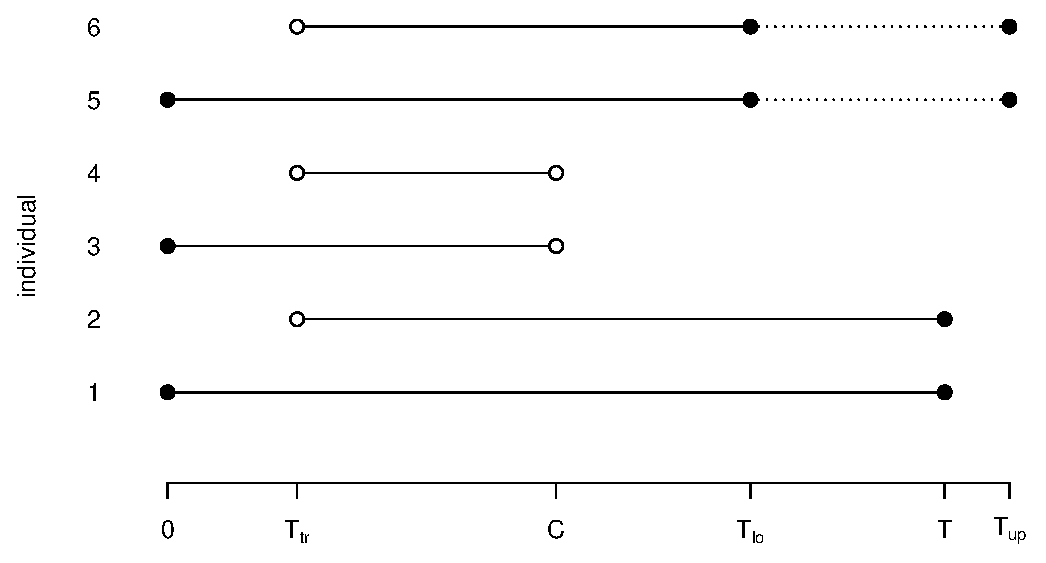
\epsfig{file=grafiken/censoringschemes.eps,scale=0.7}
{\it\caption{Illustration of different censoring
schemes.\label{censoringschemes}}}
\end{center}
\end{figure}

In a general framework an observation can now be uniquely described
 by the quadruple $(T_{tr},T_{lo},T_{up},\delta)$, with
\begin{center}
\begin{tabular}{ll}
$T_{lo}=T_{up}=T$, $\delta=1$ & if the observation is uncensored,\\
$T_{lo}=T_{up}=C$, $\delta=0$ & if the observation is right censored,\\
$T_{lo}<T_{up}$, $\delta=0$ & if the observation is interval censored.\\
\end{tabular}
\end{center}
For left truncated observations we have $T_{tr}>0$ while $T_{tr}=0$
for observations which are not truncated.

Based on these definitions we can now construct the likelihood
contributions for the different censoring schemes in terms of the
hazard rate $\lambda(t)$ and the survivor function
$S(t)=\exp(\int_0^t\lambda(u)du)$. Under the common assumption of
noninformative censoring and conditional independence, the
likelihood is given by
\begin{equation}\label{likelihood}
 L=\prod_{i=1}^n L_i,
\end{equation}
where
\[L_i = \lambda(T_{up})S(T_{up})/S(T_{tr}) = \lambda(T_{up})\exp\left(-\int_{T_{tr}}^{T_{up}}\lambda(t)dt\right)\]
for an uncensored observation,
\[L_i = S(T_{up})/S(T_{tr}) = \exp\left(-\int_{T_{tr}}^{T_{up}}\lambda(t)dt\right)\]
for a right censored observation and
\[L_i = (S(T_{lo})-S(T_{up}))/S(T_{tr}) = \exp\left(-\int_{T_{tr}}^{T_{lo}}\lambda(t)dt\right)\left(1-\exp\left(-\int_{T_{lo}}^{T_{up}}\lambda(t)dt\right)\right)\]
for an interval censored observation. Note that for explicit
evaluation of the likelihood (\ref{likelihood}) some numerical
integration technique has to be employed, since none of the
integrals can in general be solved analytically.

The above notation also allows for the easy inclusion of piecewise
constant, time-varying covariates via some data augmentation. Noting
that
\[\int_{T_{tr}}^{T}\lambda(t)dt = \int_{T_{tr}}^{t_1}\lambda(t)dt + \int_{t_1}^{t_2}\lambda(t)dt + \ldots + \int_{t_{p-1}}^{t_p}\lambda(t)dt + \int_{t_p}^{T}\lambda(t)dt\]
for $T_{tr}<t_1<\ldots<t_q<T$, we can replace an observation
$(T_{tr},T_{lo},T_{up},\delta)$ by a set of new observations
$(T_{tr},t_1,t_1,0)$, $(t_1,t_2,t_2,0)$, \ldots
$(t_{p-1},t_p,t_p,0)$, $(t_{p},T_{lo},T_{up},\delta)$ without
changing the likelihood. Therefore, observations with time-varying
covariates can be split up into several observations, where the
values $t_1<\ldots<t_p$ are defined by the changepoints of the
covariate and the covariate is now time-constant on each of the
intervals. In theory, other paths for a covariate $x(t)$ than
piecewise constant ones are also possible, if $x(t)$ is known for
$T_{tr}\le t\le T_{lo}$. In this case the the likelihood
(\ref{likelihood}) can also be evaluated numerically but a general
path $x(t)$ may lead to complicated data structures.

Figure \ref{timevaryingcovs} illustrates the data augmentation step
for a left truncated, uncensored observation and a covariate $x(t)$
that takes the three different values $x_1,x_2$ and $x_3$ on the
three intervals $[T_{tr},t_1], [t_1,t_2]$ and $[t_2,T_{up}]$. Here,
the original observation $(T_{tr},T_{up},T_{up},1)$ has to be
replaced by $(T_{tr},t_1,t_1,0)$, $(t_1,t_2,t_2,0)$ and
$(t_2,T_{up},T_{up},1)$.
\begin{figure}[htb]
\begin{center}
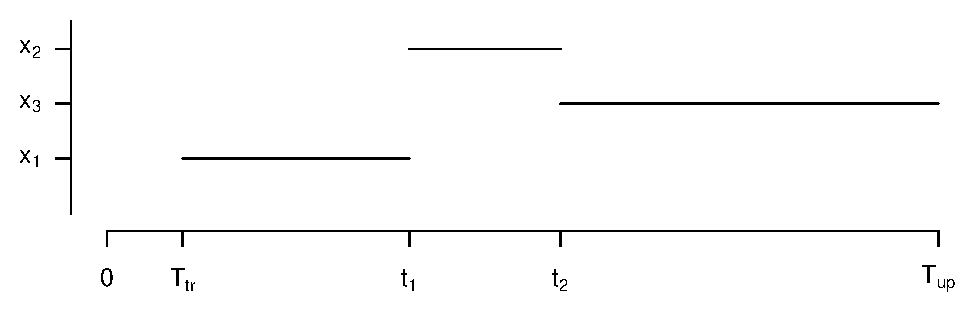
\epsfig{file=grafiken/timevaryingcovs.eps,scale=0.7}
{\it\caption{Illustration of time-varying
covariates.\label{timevaryingcovs}}}
\end{center}
\end{figure}

Currently, interval censored survival times can only be handled with
{\em remlreg objects}.

\subsection{Continuous-time multi-state models}\label{msmodels}
\index{Multi-state models}\index{Recurrent Events}\index{Disease
progression}\index{Competing risks}

Multi-state models are a flexible tool for the analysis of
time-continuous phenomena that can be characterized by a discrete
set of states. Such data structures naturally arise when observing a
discrete response variable for several individuals or objects over
time. Some common examples are depicted in Figure~\ref{some_msms} in
terms of their reachability graph for illustration. For recurrent
events (Figure~\ref{some_msms} (a)), the observations evolve through
time moving repeatedly between a fixed set of states. Other model
classes involve absorbing states, for example disease progression
models (Figure~\ref{some_msms} (b)), that are used to describe the
chronological development of a certain disease. If the severity of
this disease can be grouped into $q-1$ ordered stages of increasing
severity, a reasonable model might look like this: Starting from
disease state '$j$', an individual can only move to contiguous
states, i.e. either the disease gets worse and the individual moves
to state '$j+1$', or the disease attenuates and the individual moves
to state '$j-1$'. In addition, death is included as a further,
absorbing state '$q$', which can be reached from any of the disease
states. A model with several absorbing states is the competing risks
model (Figure~\ref{some_msms} (c)) where, for example, different
causes of death are analysed simultaneously.

\begin{figure}
\begin{center}
  \vspace{3mm}
 \mbox
 {
 \beginpicture
 \setcoordinatesystem units <0.65cm,0.65cm> point at 0 0
 \setlength{\unitlength}{0.65cm}

 \put {(a) Recurrent events} [Bl] at 0 16.5

 \put {\circle{1}} [Bl] at 7.5 12
 \put {\bf3} [Bl] at 7.35 11.85

 \put {\circle{1}} [Bl] at 5.5 14.5
 \put {\circle{1}} [Bl] at 9.5 14.5
 \put {\bf1} [Bl] at 5.35 14.35
 \put {\bf2} [Bl] at 9.35 14.35

 \arrow <3mm> [0.2,0.5] from 6.3 14.65 to 8.7 14.65
 \arrow <3mm> [0.2,0.5] from 8.7 14.35 to 6.3 14.35

 \arrow <3mm> [0.2,0.5] from  5.55 13.85 to 6.9 12.65
 \arrow <3mm> [0.2,0.5] from  7.25 12.65 to 5.9 13.85

 \arrow <3mm> [0.2,0.5] from  9.1 13.85 to 7.75 12.65
 \arrow <3mm> [0.2,0.5] from  8.1 12.65 to 9.45 13.85


 \put {(b) Disease progression} [Bl] at 0 10.5

 \put {\circle{1}} [Bl] at 7.5 6
 \put {$q$} [Bl] at 7.35 5.85

 \put {\circle{1}} [Bl] at 1.5 9
 \put {\circle{1}} [Bl] at 4.5 9
 \put {\circle{1}} [Bl] at 7.5 9
 \put {\circle{1}} [Bl] at 13.5 9
 \put {\bf1} [Bl] at 1.35 8.85
 \put {\bf2} [Bl] at 4.35 8.85
 \put {\bf3} [Bl] at 7.35 8.85
 \put {$q$-1} [Bl] at 13.15 8.85

 \put{$\cdots$} [Bl] at 10.1 8.9

 \arrow <3mm> [0.2,0.5] from 2.2 9.15 to 3.8 9.15
 \arrow <3mm> [0.2,0.5] from  3.8 8.85 to 2.2 8.85

 \arrow <3mm> [0.2,0.5] from 5.2 9.15 to 6.8 9.15
 \arrow <3mm> [0.2,0.5] from  6.8 8.85 to 5.2 8.85

 \arrow <3mm> [0.2,0.5] from 8.2 9.15 to 9.8 9.15
 \arrow <3mm> [0.2,0.5] from  9.8 8.85 to 8.2 8.85

 \arrow <3mm> [0.2,0.5] from 11.2 9.15 to 12.8 9.15
 \arrow <3mm> [0.2,0.5] from  12.8 8.85 to 11.2 8.85

 \arrow <3mm> [0.2,0.5] from  7.5 8.35 to 7.5 6.65
 \arrow <3mm> [0.2,0.5] from  4.75 8.35 to 7.0 6.65
 \arrow <3mm> [0.2,0.5] from  1.75 8.35 to 6.5 6.5
 \arrow <3mm> [0.2,0.5] from  13.25 8.35 to 8.5 6.5

 \put {(c) Competing risks} [Bl] at 0 4.5

 \put {\circle{1}} [Bl] at 1.5 0
 \put {\circle{1}} [Bl] at 4.5 0
 \put {\circle{1}} [Bl] at 7.5 0
 \put {\circle{1}} [Bl] at 13.5 0
 \put {\bf2} [Bl] at 1.35 -0.15
 \put {\bf3} [Bl] at 4.35 -0.15
 \put {\bf4} [Bl] at 7.35 -0.15
 \put {$q$} [Bl] at 13.35 -0.15

 \put {\circle{1}} [Bl] at 7.5 3
 \put {\bf1} [Bl] at 7.35 2.85

 \put{$\cdots$} [Bl] at 10.1 -0.1

 \arrow <3mm> [0.2,0.5] from  7.5 2.35 to 7.5 0.65

 \arrow <3mm> [0.2,0.5] from  6.9 2.6 to 4.75 0.65
 \arrow <3mm> [0.2,0.5] from  6.5 2.75 to 1.95 0.65
 \arrow <3mm> [0.2,0.5] from  8.5 2.75 to 12.85 0.65

 \endpicture
 }
 \vspace{3mm}

 \caption{Reachability graphs of some common multi-state
 models.\label{some_msms}}
\end{center}
\end{figure}

A multi-state model is fully described by a set of hazard rates
$\lambda_{hi}(t)$ where $h$, $h=1,\ldots,k$, indexes the type of the
transition and $i$, $i=1,\ldots,n$, indexes the individuals. Since
the hazard rates describe durations between transitions, we specify
them in analogy to hazard rate models for continuous time survival
analysis. To be more specific, $\lambda_{hi}(t)$ is modelled in a
multiplicative Cox-type way as
\[
 \lambda_{hi}(t) = \exp(\eta_{hi}(t)),
\]
where
\begin{equation}\label{addpred}
 \eta_{hi}(t) = g_{h0}(t) + \sum_{l=1}^Lg_{hl}(t)u_{il}(t) +
 \sum_{j=1}^Jf_{hj}(x_{ij}(t)) + v_i(t)'\gamma_h +  b_{hi}
\end{equation}
is an additive predictor consisting of the following components:
\begin{itemize}
 \item A time-varying, nonparametric baseline effect $g_{h0}(t)$ common for all
 observations.
 \item Covariates $u_{il}(t)$ with time-varying effects $g_{hl}(t)$.
 \item Nonparametric effects $f_{hj}(x_{ij}(t))$ of continuous covariates
 $x_{ij}(t)$.
 \item Parametric effects $\gamma_h$ of covariates $v_i(t)$.
 \item Frailty terms $b_{hi}$ to account for unobserved
 heterogeneity.
\end{itemize}

For each individual $i$, $i=1,\ldots,n,$ the likelihood contribution
in a multi-state model can be derived from a counting process
representation of the multi-state model. Let $N_{hi}(t)$,
$h=1,\ldots,k$ be a set of counting processes counting transitions
of type $h$ for individual $i$. Consequently, $h=1,\ldots,k$ indexes
the observable transitions in the model under consideration and the
jumps of the counting processes $N_{hi}(t)$ are defined by the
transition times of the corresponding multi-state process for
individual $i$.

From classical counting process theory (see e.g. Andersen et al.,
1993, Ch.~VII.2), the intensity processes $\alpha_{hi}(t)$ of the
counting processes $N_{hi}(t)$ are defined as the product of the
hazard rate for type $h$ transitions $ \lambda_{hi}(t)$ and a
predictable at-risk indicator process $Y_{hi}(t)$, i.e.
\[
 \alpha_{hi}(t) = Y_{hi}(t) \lambda_{hi}(t),
\]
where the hazard rates are constructed in terms of covariates as in
(\ref{addpred}). The at-risk indicator $Y_{hi}(t)$ takes the value
one if individual $i$ is at risk for a type $h$ transition at time
$t$ and zero otherwise. For example, in the multi-state model of
Figure~\ref{some_msms}a), an individual in state 2 is at risk for
both transitions to state 1 and state 3. Hence, the at-risk
indicators for both the transitions '2 to 1' and '2 to 3' will be
equal to one as long as the individual remains in state 2.

Under mild regularity conditions, the individual log-likelihood
contributions can now be obtained from counting process theory as
\begin{equation}\label{loglike1}
 l_i = \sum_{h=1}^k\left[ \int_0^{T_i}\log(\lambda_{hi}(t))dN_{hi}(t) -
 \int_0^{T_i}\lambda_{hi}(t)Y_{hi}(t)dt\right],
\end{equation}
where $T_i$ denotes the time until which individual $i$ has been
observed. The likelihood contributions can be interpreted similarly
as with hazard rate models for survival times (and in fact coincide
with these in the case of a multi-state process with only one
transition to an absorbing state). The first term corresponds to
contributions at the transition times since the integral with
respect to the counting process in fact equals a simple sum over the
transition times. Each of the summands is then given by the
log-intensity for the observed transition evaluated at this
particular time point. In survival models this term simply equals
the log-hazard evaluated at the survival time for uncensored
observations. The second term reflects cumulative intensities
integrated over accordant waiting periods between two successive
transitions. The integral is evaluated for all transitions the
corresponding person is at risk at during the current period. In
survival models there is only one such transition (the transition
from 'alive' to 'dead') and the integral is evaluated from the time
of entrance to the study to the survival or censoring time.

More details on multi-state models, including an exemplary analysis
on human sleep, can be found in Kneib and Hennerfeind (2006)

\section{References}
\label{bayesregref}

\begin{description}
\item[Albert, J. and Chib, S., (1993):]
Bayesian analysis of binary and polychotomous response data. {\it
Journal of the American Statistical Association},  88, 669-679.

\item[Andersen, P. K., Borgan, {\O}, Gill, R. D. and Keiding, N. (1993):]
{\it Statistical Models Based on Counting Processes,} Springer.

\item[Andrews, D.F. and Mallows, C.L. (1974):]
Scale mixtures of normal distributions. {\it Journal of the Royal
Statistical Society B}, 36, 99-102.

\item[Bollaerts, K. and Eilers, P. and Van Mechelen, I. (2006):]
Simple and Multiple P-Spline Regression with Shape Constraints.
{\it British Journal of Mathematical and Statistical Psychology},
59, 451--469.

\item[Belitz, C. (2007):] {\it Model selection in Generalised Structured Additive Regression Models.} Dr. Hut Verlag, M\"{u}nchen.

\item[Belitz, C.  and Lang, S. (2007):] Simultaneous selection of variables and smoothing parameters
in structured additive regression models. Revised for {\em Computational Statistics and Data Analysis}.


\item[Brezger, A. and Lang, S., (2006):]
Generalized additive regression based on Bayesian P-splines. {\it
Computational Statistics and Data Analysis}, 50, 967-991.

\item[Devroye, L. (1986):]
{\it Non-Uniform Random Variate Generation.} Springer-Verlag, New
York.

\item[Eilers, P. H. C. and Marx, B. D. (1996):]
Flexible smoothing using B-splines and penalized likelihood.
{\it Statistical Science}, 11, 89--121.

\item[Fahrmeir, L., Kneib, T. and Lang, S., (2004):] Penalized
structured additive regression for space-time data: a Bayesian
perspective. {\em Statistica Sinica}, 14, 715-745.

\item[Fahrmeir, L. and Lang, S. (2001a):] Bayesian Inference for
Generalized Additive Mixed Models Based on Markov Random Field
Priors. {\em Journal of the Royal Statistical Society C}, 50,
201-220.

\item[Fahrmeir, L. and Lang, S. (2001b):] Bayesian Semiparametric Regression Analysis of Multicategorical
Time-Space Data. {\em Annals of the  Institute of Statistical
Mathematics}, 53, 10-30.

\item[Fahrmeir, L. and Osuna, L. (2006):] Structured additive regression for
overdispersed and zero-inflated count data. {\em Applied Stochastic
Models in Business and Industry}, 22, 351-369.

\item[Fahrmeir, L. and Tutz, G. (2001):] {\em Multivariate Statistical
Modelling based on Generalized Linear Models.} New York:
Springer--Verlag.

\item[Fotheringham, A.S., Brunsdon, C., and Charlton, M.E., 2002:]
{\it Geographically Weighted Regression: The Analysis of Spatially
Varying Relationships.} Wiley, Chichester.

\item[Gamerman, D. (1997):] Efficient Sampling from the posterior distribution
in generalized linear models. {\em Statistics and Computing}, 7,
57-68.

\item[Gelfand, A.E., Sahu, S.K. and Carlin, B.P. (1996):] Efficient Parametrizations for
Generalized Linear Mixed Models. In: Bernardo, J.M., Berger, J.O.,
Dawid, A.P. and Smith, A.F.M. (eds.), {\em Bayesian Statistics,
5}. Oxford University Press, 165-180.

\item[George, A. and Liu, J. W. (1981).] {\em Computer Solution of Large
Sparse Positive Definite Systems.} Series in computational
mathematics, Prentice--Hall.

\item[Green, P.J. (1987):] Penalized
likelihood for general semiparametric regression models. {\it
International Statistical Review}, 55, 245--259.

\item[Green, P.J. (2001):] A Primer in Markov Chain Monte Carlo. In: Barndorff-Nielsen, O.E.,
Cox, D.R. and Kl\"{u}ppelberg, C. (eds.), {\em Complex Stochastic
Systems}. Chapmann and Hall, London, 1-62.

\item[Green, P.J. and Silverman, B. (1994):] {\em Nonparametric Regression and Generalized Linear Models.} Chapman
and Hall, London.

\item[Harville, D. A. (1977):]
Maximum Likelihood approaches to variance component estimation and
to related problems. {\it Journal of the American Statistical
Association}, 72, 320--338.

\item[Hastie, T. and Tibshirani, R. (1990):] {\em Generalized additive models.} Chapman and
Hall, London.

\item[Hastie, T. and Tibshirani, R. (1993):] Varying-coefficient Models.
{\em Journal of the Royal Statistical Society B} , 55, 757-796.

\item[Hastie, T. and Tibshirani, R. (2000):] Bayesian Backfitting. {\em Statistical Science}, 15, 193-223.

\item[Hastie, T., Tisbshirani, R. and Friedman, J. (2001):] {\em The Elements of Statistical Learning: Data Mining,
Inference and Prediction.} New York: Springer--Verlag.

\item[Hennerfeind, A., Brezger, A., Fahrmeir, L. (2006):]
Geoadditive Survival models. {\em Journal of the American
Statistical Association}, 101, 1065-1075.

\item[Holmes, C., Held, L. (2006):]
Bayesian auxiliary variable models for binary and multinomial
regression. {\em Bayesian Analysis}, 1, 145-168.

\item[Hurvich, C. M., Simonoff, J.S. and Tsai, C.L. (1998):]
Smoothing parameter selection in nonparametric regression using an
                    improved {A}kaike information criterion,
{\it Journal of the Royal Statistical Society B}, 60, 271--293.



\item[Johnson, M.E., Moore, L.M. and
Ylvisaker, D., (1990):] Minimax and maximin designs. {\it Journal of
Statistical Planning and Inference} , 26, 131-148.

\item[Kammann, E. E. and Wand, M. P., (2003):] Geoadditive Models. {\it Journal of the Royal
Statistical Society C}, 52, 1-18.

\item[Kneib, T. (2006):] Geoadditive hazard regression for interval
censored survival times. {\em Computational Statistics and Data
Analysis}, 51, 777-792

\item[Kneib, T. and Hennerfeind, A. (2006):] Bayesian Semiparametric
Multi-State Models. Under revision for {\em Statistical Modelling}.
A preliminary version is available as SFB 386 Discussion Paper 502.

\item[Kneib, T. and Fahrmeir, L. (2006):] Structured additive
regression for categorical space-time data: A mixed model approach.
{\it Biometrics}, 62, 109-118.

\item[Kneib, T. and Fahrmeir, L. (2007):] A mixed model approach
to structured hazard regression. {\em Scandinavian Journal of
Statistics}, 34, 207-228..

\item[Knorr-Held, L. (1999):] Conditional Prior Proposals in
Dynamic Models. {\em Scandinavian Journal of Statistics}, 26,
129-144.

\item[Kragler, P. (2000):] \href{http://www.scor.fr/us/2_laureat.asp?pays=2}
{Statistische Analyse von Schadensf\"allen privater
Krankenversicherungen.} Master thesis, University of Munich.

\item[Lang, S. and Brezger, A. (2004):] Bayesian P-splines. {\it
Journal of Computational and Graphical Statistics}, 13, 183-212.

\item[Lin, X. and Zhang, D., (1999):]
Inference in generalized additive mixed models by using smoothing
splines. {\it Journal of the Royal Statistical Society B}, 61,
381-400.

\item[McCullagh, P. and Nelder, J.A. (1989):] {\em Generalized Linear Models.} Chapman and Hall, London.

\item[Nychka, D. and Saltzman, N., (1998):]
{\it Design of Air-Quality Monitoring Networks},
Lecture Notes in Statistics, 132, 51--76.

\item[Osuna, L. (2004):] {\it Semiparametric Bayesian Count Data
Models}, Dr. Hut Verlag, M\"{u}nchen.

\item[Rue, H. (2001):] Fast Sampling of Gaussian Markov Random Fields with Applications.
{\em Journal of the Royal Statistical Society B}, 63, 325-338.

\item[Spiegelhalter, D.J., Best, N.G., Carlin, B.P. and van der Linde, A. (2002):]
Bayesian measures of model complexity and fit. {\em Journal of the
Royal Statistical Society B}, 65, 583-639.

\end{description}

\addcontentsline{toc}{section}{Index}
\documentclass[11pt,a4paper,twoside]{bayesxarticle}


\usepackage{amsfonts}
\usepackage[dvips]{graphicx}
\usepackage[dvips]{epsfig}
\usepackage{fancyhdr}
\usepackage{dsfont}
\usepackage{amsmath}
\usepackage{dsfont}
\usepackage{amssymb}

%\usepackage{showkeys}
%\usepackage{showidx}

\usepackage{rotating}
\usepackage{shortvrb}
\usepackage{multicol}
\usepackage{longtable}
\usepackage{xr}

\usepackage[ps2pdf]{thumbpdf}
\usepackage[ps2pdf]{hyperref}

\input{prepictex}
\input{pictexwd}
\input{postpictex}

\hypersetup{
%    pdffitwindow=true,
    pdfstartview=FitB,
    pdftitle={BayesX Manuals},
    pdfauthor={Christiane Belitz, Andreas Brezger, Thomas Kneib, Stefan Lang and Nikolaus Umlauf},
    colorlinks=true,
    linkcolor=blue,
    pdfpagemode=UseOutlines,
    bookmarksopen=true,
    bookmarksnumbered=true,
    pdfstartpage={1},
    hyperindex=true
    }

\usepackage[dcu]{harvard}

\sloppy
\parindent0em
\parskip0.3em
\topmargin -0.3cm \textheight24cm \textwidth16.5cm \headheight0.5cm \oddsidemargin-0.4cm \evensidemargin-0.4cm

 \fancyhead[RO,LE]{\thepage}
 \fancyhead[C]{}
 \fancyhead[LO]{\nouppercase\rightmark}
 \fancyhead[RE]{\nouppercase\leftmark}
 \fancyfoot[RO,LE]{}
 \fancyfoot[C]{\small\today} %Am ende raus!!!
 \fancyfoot[LO,RE]{}
 \fancyfoot[C]{}

 \renewcommand{\headrulewidth}{.4pt}
 \renewcommand{\footrulewidth}{0pt} %Am Ende 0 !!!

\pagestyle{fancy}


\renewcommand{\descriptionlabel}[1]{\hspace\labelsep\sc #1}

 \newcommand{\Cov}{\mbox{Cov}}
 \newcommand{\diag}{\mbox{diag}}
 \newcommand{\trace}{\mbox{trace}}
 \newcommand{\df}{\mbox{df}}

\def \re {{\bf R}}
\def \beq {\begin{equation}}
\def \eeq {\end{equation}}
\def \bdis {\begin{displaymath}}
\def \edis {\end{displaymath}}
\def \ds {\displaystyle}

\def \mbeta {\mbox{\boldmath $\beta$}}
\def \mtheta {\mbox{\boldmath $\theta$}}
\def \hatmbeta {\mbox{\boldmath $\hat\beta$}}
\def \eps {\epsilon}
\def \meps {\mbox{\boldmath $\epsilon$}}
\def \mmu {\mbox{\boldmath $\mu$}}
\def \mnu {\mbox{\boldmath $\nu$}}
\def \mSigma {\mbox{\boldmath $\Sigma$}}
\def \mGamma {\mbox{\boldmath $\Gamma$}}
\def \msigma {\mbox{\boldmath $\sigma$}}
\def \mPhi {\mbox{\boldmath $\Phi$}}
\def \Sigmavec {\mbox{\boldmath $\Sigma$}}
\def \sigmavec {\mbox{\boldmath $\sigma$}}
\def \nuvec {\mbox{\boldmath $\nu$}}
\def \tauvec {\mbox{\boldmath $\tau$}}




\newcommand{\N}{\mbox{N}}
\newcommand{\Var}{\mbox{Var}}
\newcommand{\E}{\mbox{E}}

\newcommand{\X}{\mbox{\boldmath $X$}}
\newcommand{\x}{\xvec}
\newcommand{\Z}{\mbox{\boldmath $Z$}}
\newcommand{\z}{\mbox{\boldmath $z$}}
\newcommand{\mb}{\mbox{\boldmath $b$}}
\newcommand{\Fx}{\mbox{\scriptsize \boldmath $x$}}
\newcommand{\I}{\mbox{\boldmath $I$}}
\newcommand{\Y}{\mbox{\boldmath $Y$}}
\newcommand{\y}{\mbox{\boldmath $y$}}
\newcommand{\mS}{\mbox{\boldmath $S$}}
\newcommand{\T}{\mbox{\boldmath $T$}}
\newcommand{\K}{\mbox{\boldmath $K$}}
\newcommand{\kt}{\mbox{\boldmath $t$}}
\newcommand{\U}{\mbox{\boldmath $U$}}
\newcommand{\fu}{\mbox{\boldmath $u$}}
\newcommand{\ba}{\mbox{\boldmath $\alpha$}}
\newcommand{\bb}{\mbox{\boldmath $\beta$}}

\def \Mvec {\vec{M}}
\def \Kvec {\vec{K}}
\def \mM {\vec{M}}
\def \Pvec {\vec{P}}
\def \Svec {\vec{S}}
\def \deltavec {\vec{\delta}}
\def \lambdavec {\boldsymbol{\lambda}}
\def \Lambdavec {\boldsymbol{\Lambda}}
\def \betavec {\boldsymbol{\beta}}
\def \etavec {\boldsymbol{\eta}}
\def \gammavec {\boldsymbol{\gamma}}
\def \Gammavec {\boldsymbol{\Gamma}}
\def \Omegavec {\boldsymbol{\Omega}}
\def \muvec {\boldsymbol{\mu}}
\def \kappavec {\boldsymbol{\kappa}}
\def \nuvec {\boldsymbol{\nu}}
\def \pivec {\vec{\pi}}
\def \thetavec {\vec{\theta}}
\def \varthetavec{\vec{\vartheta}}
\def \varepsilonvec {\boldsymbol{\varepsilon}}
\def \zetavec {\vec{\zeta}}
\def \Sigmavec {\boldsymbol{\Sigma}}
\def \Thetavec {\boldsymbol{\theta}}

\def \dvec {\mathbf{d}}
\def \fvec {\mathbf{f}}
\def \fhatvec {\mathbf{\hat{f}}}
\def \svec {\mathbf{s}}
\def \wvec {\mathbf{w}}
\def \xvec {\mathbf{x}}
\def \yvec {\mathbf{y}}
\def \uvec {\mathbf{u}}
\def \avec {\mathbf{a}}
\def \zvec {\mathbf{z}}
\def \bvec {\mathbf{b}}
\def \tvec {\mathbf{t}}
\def \mvec {\mathbf{m}}
\def \cvec {\mathbf{c}}

\def \ds {\displaystyle}

\def \Gvec {\mathbf{G}}
\def \Rvec {\mathbf{R}}
\def \Avec {\mathbf{A}}
\def \Bvec {\mathbf{B}}
\def \Cvec {\mathbf{C}}
\def \Dvec {\mathbf{D}}
\def \Fvec {\mathbf{F}}
\def \Kvec {\mathbf{K}}
\def \Hvec {\mathbf{H}}
\def \Ivec {\mathbf{I}}
\def \Lvec {\mathbf{L}}
\def \Uvec {\mathbf{U}}
\def \Wvec {\mathbf{W}}
\def \Yvec {\mathbf{Y}}
\def \Zvec {\mathbf{Z}}
\def \svec {\mathbf{s}}
\def \Cvec {\mathbf{C}}
\def \dvec {\mathbf{d}}
\def \Avec {\mathbf{A}}
\def \Pvec {\mathbf{P}}
\def \Vvec {\mathbf{V}}
\def \xivec {\mathbf{x_i}}
\def \xjvec {\mathbf{x_j}}
\def \betavecr {\vec{\beta_r}}
\def \betavec {\boldsymbol{\beta}}
\def \betadach {\hat{\vec{\beta}}}
\def \betadachr {\vec{\hat{\beta}_r}}
\def \betaschl {\vec{\tilde{\beta}}}
\def \betaschlr {\vec{\tilde{\beta}_r}}
\def \sschlr {\vec{\tilde{s}_r}}
\def \Aschlr {\vec{\tilde{A}_r}}
\def \Adach {\vec{\hat{A}}}
\def \Avecr {\vec{A}_r}
\def \Adachr {\vec{\hat{A}_r}}
\def \Fdach {\vec{\hat{F}}}
\def \Vdach {\vec{\hat{V}}}
\def \Aschl {\vec{\tilde{A}}}
\def \Xvec {\mathbf{X}}

\def \nullvec {\boldsymbol{0}}

\def \hvec {\vec{h}}
\def \vvec {\vec{v}}
\def \wvec {\vec{w}}
\def \x1vec {\vec{x_1}}
\def \xnvec {\vec{x_n}}

\def \Kmat {\mathbf{K}}
\def \Kmatj {\mathbf{K}_j}
\def \Xmat {\mathbf{X}}
\def \Vmat {\mathbf{V}}
\def \Smat {\mathbf{S}}


\def \dsR {\text{$\mathds{R}$}}
 \DeclareMathOperator{\B}{B}

\def \einsvec {\boldsymbol{1}}

\newcommand{\subheader}[1]{\textsf{\textbf{{\large #1}}}}

\newenvironment{stanza}[2]{\subheader{#1} \begin{itemize} \item[]#2}{\end{itemize}}


\newcommand{\preface}[1]{
\thispagestyle{empty}

\begin{center}
{\bf \em \huge BayesX}

\vspace{0.5cm}

{\em \large Software for Bayesian Inference in Structured Additive Regression Models}

\vspace{0.5cm}

{\em Version 2.1}

\vspace{0.5cm}

\begin{figure}[h]
\begin{center}
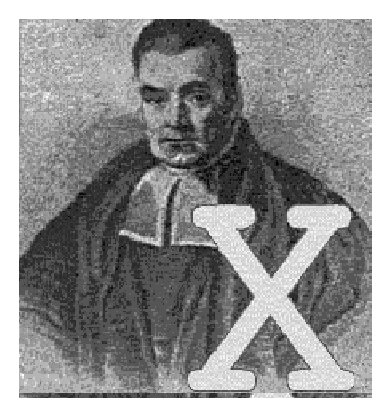
\includegraphics[scale=1.2]{grafiken/bayesicon.eps}
\end{center}
\end{figure}

\vfill

{\bf\sffamily \huge #1}

\vfill

\end{center}

{\em Developed by}

Christiane Belitz\\
Andreas Brezger\\
Thomas Kneib (University of G{\"o}ttingen)\\
Stefan Lang (University of Innsbruck) \\
Nikolaus Umlauf (University of Innsbruck) \\

\vspace{2ex}

{\em With contributions by}

\vspace{-1.5ex}

\begin{multicols}{2}
Daniel Adler
Eva-Maria Fronk\\
Felix Heinzl\\
Andrea Hennerfeind\\
Manuela Hummel\\
Alexander Jerak\\
Susanne Konrath\\
Petra Kragler\\
Cornelia Oberhauser\\
Leyre Est\'{\i}baliz Osuna Echavarr\'{\i}a\\
Daniel Saban\'{e}s Bov\'{e} \\
Achim Zeileis
\end{multicols}

{\em Supported by}

Ludwig Fahrmeir (mentally)\\
Leo Held (mentally)\\
German Research Foundation (DFG)

\newpage

\subsection*{Acknowledgements}

The development of {\em BayesX} has been supported by grants from the German Research Foundation (DFG), Collaborative
Research Center 386 ``Statistical Analysis of Discrete Structures''.

Special thanks go to (in alphabetical order of first names):

{\em Dieter Gollnow} for computing and providing the map of Munich (a really hard job); \\
{\em Leo Held} for advertising the program; \\
{\em Ludwig Fahrmeir} for his patience with finishing the program and for carefully
reading and correcting the  manual; \\
{\em Ngianga-Bakwin Kandala} for being the first user of the program (a really hard job); \\
{\em Samson Babatunde Adebayo} for carefully reading and correcting the manual; \\
{\em Ursula Becker} for carefully reading and correcting the manual;

\subsection*{Licensing agreement}

This program is free software; you can redistribute it and/or
modify it under the terms of the GNU General Public License
as published by the Free Software Foundation; either version 2
of the License, or (at your option) any later version.

This program is distributed in the hope that it will be useful,
but WITHOUT ANY WARRANTY; without even the implied warranty of
MERCHANTABILITY or FITNESS FOR A PARTICULAR PURPOSE.  See the
GNU General Public License for more details.

You should have received a copy of the GNU General Public License
along with this program; if not, write to the Free Software
Foundation, Inc., 51 Franklin Street, Fifth Floor, Boston, MA  02110-1301, USA.



\vspace{0.5cm}

{\em BayesX} is available at { \href{http://www.bayesx.org}{http://www.bayesx.org}}}


 \externaldocument{manual}
 \externaldocument{manual_tutorials}

 \makeindex

\begin{document}
\MakeShortVerb{\#}

\preface{Methodology Manual}

\newpage

\section{Introduction}

In this manual we provide a brief review of the methodological background for the three regression tools currently implemented
in {\em BayesX}. The first regression tool ({\em bayesreg objects}) relies on Markov chain Monte Carlo (MCMC) simulation
techniques and yields fully Bayesian posterior mean or posterior mode estimates. The second regression tool ({\em remlreg
objects}) is based on the mixed model representation of penalised regression models with inference being based on penalised
maximum likelihood and marginal likelihood (a generalisation of restricted maximum likelihood) estimation. The third regression
tool ({\em stepwisereg objects}) simultaneously performs model choice and estimation with inference being based on penalised
likelihood. MCMC techniques are partly used for computing interval estimates. All regression tools allow to estimate structured
additive regression (STAR) models (\citeasnoun{BelLan08}, \citeasnoun{BreLan06}, \citeasnoun{FahKneLan04}) with complex semiparametric predictors.
STAR models cover a number of well
known model classes as special cases, including {\em generalized additive models} \cite{HasTib90}, {\em generalized additive
mixed models} \cite{LinZha99}, {\em geoadditive models} \cite{KamWan03}, {\em varying coefficient models}\cite{HasTib93}, and
{\em geographically weighted regression} \citeasnoun{FotBruCha02}. Besides models for responses from univariate exponential
families, BayesX also supports non-standard regression situations such as models for categorical responses with either ordered
or unordered categories, continuous time survival data, or continuous time multi-state models. To provide a first impression of
structured additive regression, Sections~\ref{obsmodel} to \ref{inference} describe STAR models for exponential family
regression. Section~\ref{survivalAnalysis} extends structured additive regression to the analysis of survival times and
multi-state data. Full details on STAR methodology can be found in the following references:

\subsubsection*{Structured additive regression based on MCMC
simulation}

\begin{itemize}
\item Brezger, A., Lang, S. (2006): Generalized structured additive regression based on Bayesian P-Splines. {\it
    Computational Statistics and Data Analysis}, {\bf 50}, 967--991.
    \vspace{-0.25cm}
\item Brezger, A., Lang, S. (2008)
      Simultaneous Probability statements for Bayesian P-splines.
      {\it Statistical Modelling}, {\bf 8},
      141--168.\vspace{-0.25cm}
\item Brezger, A., Steiner, W. (2008)
Monotonic regression based on Bayesian P-splines: an
application to estimating price response functions from
store-level scanner data. {\it Journal of Economic and Business Statistics}, {\bf 26}, 90--104.
\vspace{-0.25cm}
\item Fahrmeir, L., Lang, S. (2001): Bayesian Inference for Generalized Additive Mixed Models Based on Markov Random Field
    Priors. {\it Journal of the Royal Statistical Society C (Applied Statistics)}, {\bf 50}, 201--220.\vspace{-0.25cm}
\item Fahrmeir, L., Lang, S. (2001): Bayesian Semiparametric Regression Analysis of Multicategorical Time-Space Data. {\it
    Annals of the Institute of Statistical Mathematics}, {\bf 53}, 10--30.\vspace{-0.25cm}
\item Fahrmeir, L., Osuna, L.. (2006): Structured additive regression for overdispersed and zero-inflated count data. {\it
    Applied Stochastic Models in Business and Industry}, {\bf 22}, 351--369.\vspace{-0.25cm}
\item Hennerfeind, A., Brezger, A., Fahrmeir, L. (2006): Geoadditive survival models. {\it Journal of the American
    Statistical Association}, {\bf 101}, 1065--1075.\vspace{-0.25cm}
\item Kneib, T., Hennerfeind, A. (2006) Bayesian Semiparametric Multi-State Models. {\it Statistical Modelling}, {\bf 8},
    169--198..\vspace{-0.25cm}
\item Lang, S., Brezger, A. (2004): Bayesian P-Splines {\it Journal of Computational and Graphical Statistics}, {\bf 13},
    183--212.
\end{itemize}

Presumably the best starting point is the paper by \citeasnoun{BreLan06}.

\begin{figure}[ht]
\footnotesize
\begin{center}
%\begin{tabular}{|p{8cm}|p{5cm}|}
%\hline
%{\bf Intended use} & {\bf recommended sections } \\
%\hline
%semiparametric regression, fully Bayesian approach  & sections \ref{obsmodel}, \ref{priorassumptions} , \ref{fullbayes} \\
%\hline
%semiparametric regression, inference based on mixed model technology, classical perspective &
%sections \ref{obsmodel}, \ref{penalizedleastsquares}, \ref{glmmrep}, \ref{glmmmeth} \\
%\hline
%semiparametric regression, inference based on mixed model technology, Bayesian point of view & sections \ref{obsmodel}, \ref{priorassumptions},
%\ref{glmmrep}, \ref{glmmmeth} \\
%\hline
%semiparametric regression including model choice & sections \ref{obsmodel}, \ref{penalizedleastsquares}, \ref{stepwiseest} \\
%\hline
%\end{tabular}
% \vspace{3mm}
\[\mbox{
 \beginpicture
 \setcoordinatesystem units <1.1cm,1.1cm> point at 0 0
 \setlength{\unitlength}{1.1cm}

 \put {\framebox(5.5,0.7){\sffamily\bfseries 2 Generalized regression models}} at 0 0

 \put {Bayesian perspective} at -4 -1.2
 \put {frequentist perspective} at 4 -1.2

 \arrow <4mm> [0.25,0.75] <0pt,5mm> from 0 -1 to -5 -2.9
 \arrow <4mm> [0.25,0.75] <0pt,5mm> from 0 -1 to 5 -2.9

 \put {\framebox(4.5,0.7){\sffamily\bfseries 4 Bayesian point of view}} at -5 -3

 \put {\framebox(4.5,0.7){\sffamily\bfseries 3 Penalised likelihood}} at 5 -3

 \arrow <4mm> [0.25,0.75] <0pt,5mm> from -5 -4 to 0 -6
 \arrow <4mm> [0.25,0.75] <0pt,5mm> from 5 -4 to 0 -6

 \put {relation to mixed models} at 0 -4.5

 \put {\framebox(5.5,0.7){\sffamily\bfseries 5 Mixed model representation}} at 0 -6

 \arrow <4mm> [0.25,0.75] <0pt,5mm> from -5 -4 to -5 -9
 \arrow <4mm> [0.25,0.75] <0pt,5mm> from 5 -4 to 5 -9

 \put {\framebox(3.5,0.7){\sffamily\bfseries 6.1 bayesreg objects}} at -5 -9
 \put {\framebox(3.5,0.7){\sffamily\bfseries 6.3 stepwisereg objects}} at 5 -9

 \put {MCMC (full Bayes)} at -6.5 -6
 \put {penalised likelihood} at 6.5 -5.75
 \put {incl. model choice} at 6.5 -6.15

 \arrow <4mm> [0.25,0.75] <0pt,5mm> from 0 -7 to 0 -9

 \put {penalised likelihood} at -1.5 -7.5
 \put {(empirical Bayes)} at 1.3 -7.5

 \put {\framebox(3.5,0.7){\sffamily\bfseries 6.2 remlreg objects}} at 0 -9


 \endpicture
}\]
 \vspace{3mm}

{\em \caption {\label{guideline} Guidelines for reading this
manual.}}
\end{center}
\end{figure}

\subsubsection*{Structured additive regression based on mixed model
methodology}

\begin{itemize}
\item Fahrmeir, L., Kneib, T., Lang, S. (2004): Penalized structured additive regression for space-time data: a Bayesian
    perspective. {\it Statistica Sinica}, {\bf 14}, 715--745.\vspace{-0.25cm}
\item Kneib, T. (2006): Mixed model based inference in structured additive regression. Dr. Hut Verlag, M\"{u}nchen. Available
    online from
    \href{http://edoc.ub.uni-muenchen.de/archive/00005011/}{http://edoc.ub.uni-muenchen.de/archive/00005011/}\vspace{-0.25cm}
\item Kneib, T. (2006): Geoadditive hazard regression for interval censored survival times. {\it Computational Statistics
    and Data Analysis}, {\bf 51}, 777--792.\vspace{-0.25cm}
\item Kneib, T., Fahrmeir, L. (2007): A mixed model approach for geoadditive hazard regression. {\it Scandinavian Journal
    of Statistics}, {\bf 34}, 207--228.\vspace{-0.25cm}
\item Kneib, T., Fahrmeir, L. (2006): Structured additive regression for multicategorical space-time data: A mixed model
    approach. {\it Biometrics}, {\bf 62}, 109--118.\vspace{-0.25cm}
\item Kneib, T., Hennerfeind, A. (2006): Bayesian Semiparametric Multi-State Models. {\it Statistical Modelling}, {\bf 8},
    169--198.
\end{itemize}

Presumably the best starting point is the paper by \citeasnoun{FahKneLan04} or the monograph by \citeasnoun{Kne06}.

\subsubsection*{Structured additive regression including model selection}

\begin{itemize}
\item Belitz, C. (2007): Model selection in Generalised Structured Additive Regression Models. Dr. Hut Verlag, M\"{u}nchen.
\item Belitz, C., Lang, S. (2008) Simultaneous selection of variables and smoothing parameters
in structured additive regression models. {\it
Computational Statistics and Data Analysis}, {\bf 53} , 61-81.
\end{itemize}

Presumably the best starting point is the paper by \citeasnoun{BelLan08}.

\subsubsection*{Guideline for the reader}


The rest of this manual is organized as follows:

The next section describes the general structure of STAR models for
distributions of the response variable belonging to an exponential
family. The following Sections \ref{penalizedleastsquares} -
\ref{inference} discuss alternative approaches for specifying and
estimating the different model terms in STAR models. Section
\ref{penalizedleastsquares} describes the models from a more
classical penalized least squares perspectives. A Bayesian point of
view is taken in Section \ref{priorassumptions}. The close
connection to mixed models is highlighted in Section \ref{glmmrep}.
Section \ref{inference} gives a brief outline of the various
inference techniques for STAR models. Fully Bayesian inference via
MCMC simulation techniques is the topic of Section \ref{fullbayes}.
Inference based on mixed model technology is sketched in Section
\ref{glmmmeth}. Simultaneous selection of relevant model terms and
estimation of the parameters is described in Section
\ref{stepwiseest}.

For most users of BayesX it is sufficient to read only parts of this
manual. Some recommendations are given in Figure \ref{guideline}.


\section{Generalized regression models}
\label{obsmodel}

\index{Generalized linear model}\index{Exponential family}
Generalized linear models assume that, given covariates $\uvec$ and
unknown parameters $\gammavec$, the distribution of the response
variable $y$ belongs to an exponential family, i.e.
\begin{equation}
\label{likel} p(y \, | \, \uvec) = \exp \left( \frac{y \theta -
b(\theta)}{\phi} \right) c(y,\phi)
\end{equation}
where $b(\cdot)$, $c(\cdot)$, $\theta$ and $\phi$ determine the specific response distribution. A list of the most common
distributions and their parameters can be found for example in \citeasnoun{FahTut01}, page 21. The mean
$\mu=E(y|\uvec,\gammavec)$ is linked to a linear predictor $\eta$ by
\begin{equation}
\label{glm} \mu=h(\eta) \qquad \eta= \uvec'\gammavec,
\end{equation}
where $h$ is a known response function and $\gammavec$ are unknown
regression parameters.

In most practical regression situations, however, we are facing at
least one of the following problems:
\begin{itemize}
\item For the {\em continuous covariates} in the data set, the assumption of a strictly linear
effect on the predictor may be not appropriate. \vspace{-0.2cm}
\item Observations may be {\em spatially correlated}.
\vspace{-0.2cm}
\item Observations may be {\em temporally correlated}.
\vspace{-0.2cm}
\item Complex interactions may be required to model the joint effect
of some of the covariates adequately. \vspace{-0.2cm}
\item  Heterogeneity among individuals or units may be not sufficiently described by covariates. Hence,
unobserved {\em unit or cluster specific heterogeneity} has to be
considered appropriately.
\end{itemize}
To overcome these difficulties, we replace the strictly linear
predictor in (\ref{glm}) by a structured additive predictor
\begin{equation}
\label{gampred} \eta=f_{1}(x_{1})+\ldots+f_j(x_j) +
\ldots+f_{p}(x_{p})+\uvec'\gammavec,
\end{equation}
where $x_j$ denote
covariates of different type and dimension, and $f_j$ are (not
necessarily smooth) functions of the covariates. The functions $f_j$
comprise usual nonlinear effects of continuous covariates, time
trends and seasonal effects, two-dimensional surfaces, varying
coefficient models, i.i.d. random intercepts and slopes as well as
spatial effects. STAR-models cover a number of special cases
well known from the literature, in particular {\em Generalized additive models (GAM)},
{\em Generalized additive mixed models (GAM)}, {\em Geoadditive models}, {\em Multilevel models},
{\em Varying coefficient models (VCM)}, {\em ANOVA type interaction models} and {\em geographically weighted regression}.

\section{Penalized least squares}
\label{penalizedleastsquares}

In BayesX, the nonlinear functions $f_j$ are modeled by a basis
functions approach, i.e. a particular nonlinear function $f$ is
approximated by a linear combination of basis functions:
$$
f(x) = \sum_{k=1}^{K} \beta_k B_k(x)
$$
The $B_k$ are known basis functions and $\betavec =
(\beta_1,\dots,\beta_K)'$ is a vector of unknown regression
coefficients to be estimated. Note that the term basis function in
our understanding is not limited to basis functions known from
nonparametric smoothing such as B-splines but also refers to
non-standard basis functions such as indicator functions for regions
or clusters. To ensure enough flexibility, typically a large number
of basis functions is defined. To avoid overfitting, a roughness
penalty on the regression coefficients is additionally specified. We
use quadratic penalties of the form $\betavec' \Pvec(\lambdavec)
\betavec$ where $\Pvec(\lambdavec)$ is a penalty matrix. The penalty
depends on one or multiple smoothing parameters $\lambdavec$ that
govern the amount of smoothness imposed on the function $f$. Most
penalty matrices are of the particular simple form
$\Pvec(\lambdavec) = \lambda \Kvec$ where $\lambda$ is a scalar
smoothing parameter. For {\em stepwisereg objects} more complicated
penalties are sometimes possible. They are an additive combination
of penalty matrices. An example is $\Pvec(\lambdavec) = \lambda_1
\Kvec_1+\lambda_2 \Kvec_2$ where $\lambda_1$ and $\lambda_2$ are
smoothing parameters and $\Kvec_1$ and $\Kvec_2$ are penalty
matrices.

The choice of basis functions $B_1,\dots,B_K$ and penalty  $\Pvec(\lambdavec)$ depends on our prior assumptions about the smoothness
of $f$ as well as
the type and dimension of $x$. We will give specific examples below. Defining the $n \times K$ design matrix $\Xvec$ with elements
$X[i,k] = B_k(x_i)$ the
vector $\fvec = (f(x_1),\dots,f(x_n))'$ of function evaluations can be written in matrix notation as $\fvec = \Xvec \betavec$.
Accordingly,  for model (\ref{gampred}) we obtain
$$
\etavec = \Xvec_1 \betavec_1 + \ldots + \Xvec_p \betavec_p + \Uvec \gammavec +  \varepsilonvec,
$$
where $\Uvec$ is the design matrix for linear effects, $\gammavec$ is the vector of regression coefficients for linear effects, and
$\varepsilonvec$
are the vectors of observations and errors.
In the next subsections we will give specific examples for modeling the unknown functions $f_j$ or in other words for the choice of basis functions and
penalty matrices.
We start with modeling the effect of continuous covariates using splines.

\subsection{Continuous covariates}
\subsubsection{P(enalized)-splines}
Suppose first that a particular component $x$ of the covariate  is univariate and continuous. There is a considerable amount of
literature on basis functions approaches in combination with a (quadratic) roughness penalty for continuous covariates. BayesX
applies the P-splines approach introduced by \citeasnoun{EilMar96}. The approach assumes that the unknown functions can be
approximated by a polynomial spline of degree $l$ and with equally spaced knots
$$
x_{min} = \zeta_{0}  < \zeta_{1} < \dots < \zeta_{m-1} < \zeta_{m} = x_{max}
$$
over the domain of $x$. The spline can be written in terms of a linear combination of $K=m+l$ B-spline basis functions. The
columns of the design matrix $\Xvec$ are given by the B-spline basis functions evaluated at the observations $x_i$. To overcome
the well known difficulties involved with regression splines, \citeasnoun{EilMar96} suggest a relatively large number of knots
(usually between 20 to 40) to ensure enough flexibility, and to introduce a roughness penalty on adjacent regression
coefficients based on squared $r$-th order differences, i.e.
$$
\betavec' \lambda \Kvec \betavec = \lambda \sum_{k=r+1}^K (\Delta^r \beta_k)^2.
$$
The penalty matrix is given by $\Kvec =  \Dvec_r' \Dvec_r$ where $\Dvec_r$ is a $r$-th order difference matrix.
Typically, second or third order differences are used. The limiting behavior $\lambda \rightarrow \infty$ depends both on the
order of the spline
and the order of the penalty. If the order of the spline is equal to or
higher than the order of  the penalty, which is typically the case, then a polynomial
fit of degree $r-1$ is obtained in the limit.

The approach can be extended to impose monotonicity or more general shape constraints. We follow an approach proposed by
\citeasnoun{BolEilvMe06}. A sufficient condition for a decreasing spline is given by $\beta_{k} \leq \beta_{k-1}$, i.e.  a
parameter $\beta_{k}$ is less than its predecessor $\beta_{k-1}$. The simple but powerful idea  is to impose the required
constraint by expanding the penalty by an additional  term. More specifically they propose the composed penalty
$$
\Pvec(\lambdavec) =  \betavec' \left( \lambda_1 \Kvec_1 + \lambda_2 \Kvec_2 \right) \betavec
$$
where $\lambda_1$ and $\Kvec_1$ are the usual smoothing parameter
and penalty matrix for P-splines. The additional penalty matrix
$\Kvec_2$ is a diagonal matrix with entries 1 whenever the condition
$\beta_{k} \leq \beta_{k-1}$ fails and 0 otherwise. For increasing
functions, $\Kvec_2$ has to be adapted accordingly. The parameter
$\lambda_2$ is not estimated but set large enough to enforce
monotonic functions.





\subsubsection{Tensor product P-splines}
\label{tensorproductpsplines} Assume now that $\xvec$ is
two-dimensional, i.e. $\xvec = \left(x^{(1)},x^{(2)}\right)'$ with
continuous components $x^{(1)}$ and $x^{(2)}$. The aim is to extend
the univariate P-spline from the preceding section to two
dimensions. A common approach is to approximate the unknown surface
$f(x)$ by the tensor product of one dimensional B-splines, i.e.
\begin{equation}
\label{gampspline_2dimterm} f\left(x^{(1)},x^{(2)}\right) = \sum_{k=1}^{K_1}
\sum_{s=1}^{K_2} \beta_{ks} B_{1,k}(x^{(1)})
B_{2,s} (x^{(2)}),
\end{equation}
where $B_{11},\dots,B_{1K_1}$ are the basis functions in $x^{(1)}$ direction and
$B_{21},\dots,B_{2K_2}$ in $x^{(2)}$ direction.
The $n \times K = n \times K_1 K_2$ design matrix $\Xvec$ now consists of
products of basis functions.

Several alternatives are available for the penalty matrix $\Pvec(\lambdavec)$:
\begin{enumerate}
\item[a)] {\em Penalty based on first differences:} The
two-dimensional generalization of a penalty based on first
differences is given by combining row- and column wise quadratic
differences
$$
\begin{array}{l}
\displaystyle \sum_{k=2}^{K_1}\sum_{s=1}^{K_2}(\beta_{ks}-\beta_{k-1,s})^2 =
\betavec'(\Ivec_{K_2}\otimes \Dvec_1)'(\Ivec_{K_2}\otimes \Dvec_1)\betavec \\[0.4cm]
\displaystyle  \sum_{k=1}^{K_1}\sum_{s=2}^{K_2}(\beta_{ks}-\beta_{k,s-1})^2 =
\betavec'(\Dvec_2\otimes \Ivec_{K_1})'(\Dvec_2\otimes \Ivec_{K_1})\betavec \\
\end{array}
$$
to the penalty
$$
\betavec'\Pvec(\lambdavec) \betavec =  \betavec' \lambda \left[ (\Ivec_{K_2}\otimes \Dvec_1)'(\Ivec_{K_2}\otimes \Dvec_1) + (\Dvec_2\otimes \Ivec_{K_1})'
(\Dvec_2\otimes \Ivec_{K_1})\right]\betavec.
$$
Another way of expressing the penalty is given by
\begin{equation}
\label{2dpenalty}
 \betavec'\Pvec(\lambda)\betavec = \betavec'\lambda \left[\Ivec_{K_2}\otimes\Kvec_1 + \Kvec_2\otimes \Ivec_{K_1}\right]\betavec,
\end{equation}
where $\Kvec_1$ and $\Kvec_2$ are the respective one dimensional penalty matrices.
In the limit  $\lambda \rightarrow \infty$ a constant fit is obtained.
\item[b)] {\em Penalty based on second differences:} In a similar way two-dimensional penalties based on higher order differences
are constructed. A second order difference penalty is obtained if
$\Kvec_1$ and $\Kvec_2$ in (\ref{2dpenalty}) correspond to penalty
matrices based on second rather than first differences. Similar to
one dimensional P-splines the limit $\lambda \rightarrow \infty$
results in linear effects in $x^{(1)}$ and $x^{(2)}$ with an
additional interaction effect, i.e.
$$
f\left(z^{(1)},z^{(2)}\right) = c_0 + c_1 \, x^{(1)} + c_2 \,
x^{(2)} + c_3 \, x^{(1)} x^{(2)}.
$$
\item[c)] {\em Anisotropic penalty:} The two penalties considered so far are not capable of
different penalization in $x^{(1)}$ and $x^{(2)}$ direction,
respectively. Anisotropic penalties are obtained by assuming
separate smoothing parameters $\lambda_1$ and $\lambda_2$ in
$x^{(1)}$ and $x^{(2)}$ direction. The penalty is then given by
\begin{equation}
\label{penalty_eilmar}
 \betavec'\Pvec(\lambdavec) \betavec = \betavec'\left[\lambda_1 \Ivec_{K_2}\otimes\Kvec_1 + \lambda_2 \Kvec_2\otimes \Ivec_{K_1}\right]\betavec.
\end{equation}
The resulting fit in the limit $\lambda_1 \rightarrow \infty$ and
$\lambda_2 \rightarrow \infty$ depends on the penalty used to
construct $\Kvec_1$ and $\Kvec_2$. If $\Kvec_1$ and $\Kvec_2$
correspond to a first order difference penalty a constant fit is
obtained in the limit. Second order difference penalties result in a
linear fit for $f\left(x^{(1)},x^{(2)}\right)$.
\item[d)] {\em Penalties with main effects in the limit:} Sometimes it is desirable to decompose the effect of the two covariates
$x^{(1)}$ and $x^{(2)}$ into two main effects modeled by one
dimensional functions and a two-dimensional interaction effect, i.e.
\begin{equation}
\label{pspline_2dimtermmain} f \left(x^{(1)},x^{(2)}\right) =
f_1\left(x^{(1)} \right) + f_2 \left(x^{(2)}\right) + f_{1|2}\left(
x^{(1)},x^{(2)} \right).
\end{equation}
Usually a two-dimensional surface smoother  together with two
additional  one dimensional P-splines (or other smoothers) are
estimated. This approach is possible with {\em bayesreg objects} and
{\em remlreg objects}. {\em stepwisereg objects} take, however, a
different approach. We specify a two-dimensional surface based on
tensor product P-splines and compute the decomposition of the
resulting surface into main effects and the interaction effect {\em
after} estimation. Moreover, we specify a penalty that allows for a
main effects only model as a special case. This allows to
discriminate between a simple  main effects model and a more
complicated two way interactions model. A penalty that guarantees  a
main effects model in the limit is defined by the Kronecker product
of the two penalty matrices for one dimensional P-splines, i.e.
\begin{equation}
\label{penalty_kronecker}
\betavec'\Pvec(\lambda)\betavec = \betavec' \lambda \Kvec_1 \otimes \Kvec_2 \betavec.
\end{equation}
The drawback of this penalty is that the limit $\lambda \rightarrow \infty $ yields {\em unpenalized} main effects, i.e. wiggly functions.
We therefore use a modified penalty which is effectively a combination of the two  penalties  (\ref{penalty_eilmar}) and
(\ref{penalty_kronecker}). More specifically
we define
\begin{equation}
\label{penalty_comb}
\betavec'\Pvec(\lambdavec)\betavec = \betavec' \left[\frac{\lambda_1}{K_1}
\Ivec_{K_2}\otimes\Kvec_1 + \frac{\lambda_2}{K_2} \Kvec_2\otimes \Ivec_{K_1}+\lambda_3 \Kvec_1 \otimes \Kvec_2   \right] \betavec,
\end{equation}
where $\Kvec_1$ and $\Kvec_2$ are penalty matrices corresponding to one dimensional P-splines based on first or second order differences.
This penalty has the following nice properties:
\begin{itemize}
\item The limit $\lambda_3 \rightarrow \infty$ results in a mere main effects model. The main effects  are one dimensional P-splines with smoothing
parameters $\lambda_1$ and $\lambda_2$.
\item The limit $\lambda_3 \rightarrow 0$ yields the anisotropic penalty (\ref{penalty_eilmar}) as a special case.
\item The limit $\lambda_1 \rightarrow 0$ and $\lambda_2 \rightarrow 0$  yields the Kronecker product penalty
(\ref{penalty_kronecker}) as a special case.
\item The limit $\lambda_1 \rightarrow \infty$, $\lambda_2 \rightarrow \infty$ and $\lambda_3 \rightarrow \infty$ results in a main effects model with
linear or constant main effects depending on the difference order used to construct $\Kvec_1$ and $\Kvec_2$.
\end{itemize}
\end{enumerate}


\subsection{Spatial effects}

In this subsection we assume that $x$ represents the location a
particular observation pertains to. The location is typically given
in two ways. If exact locations are available $x=(x^{(1)},x^{(2)})'$
is two-dimensional and the components  $x^{(1)}$ and $x^{(2)}$
correspond to the coordinates of the location. In this case, the
spatial effect $f(x^{(1)},x^{(2)})$ could be modeled by
two-dimensional surface estimators as described in the preceding
section.

In many applications, however, exact locations are not available. Typically, a geographical map is available and $x \in \{1,\dots,K\}$ is an
index that denotes the region (e.g. district) an observation pertains to. A common approach is to assume $f(x) = \beta_x$,
i.e. separate parameters $\beta_1,\ldots,\beta_K$  for each region are estimated.
The $n \times K$ design matrix $\Xvec$ is an incidence matrix whose entry in
the $i$-th row and $k$-th column is equal to one if observation $i$ has been observed at
location $k$ and zero otherwise. To prevent overfitting a penalty based on squared differences is defined that
guarantees that parameters of neighboring regions are similar. Typically two regions are assumed to be neighbors if they share a common
boundary although other neighborhood definitions are possible. The penalty is defined as
$$
\betavec' \lambda \Kvec \betavec = \lambda\sum_{k=2}^{K}\sum_{s \in N(k), s < k}(\beta_k-\beta_s)^2,
$$
where $N(k)$ denotes all sites that are neighbors of site $k$.
The elements of the penalty matrix are given by
\begin{equation}
\label{K_mrf}
 \Kvec[s,r] = \lambda \left\{
 \begin{array}{ll}
-1 & k\neq s, k\sim s,\\
 0 & k\neq s, k \nsim s,\\
 |N(k)| & k=s.
\end{array}
\right.
\end{equation}

Depending on the prior belief on smoothness of the spatial effect
several alternatives to penalty (\ref{K_mrf}) are available. If a
very smooth effect is assumed, the two-dimensional smoothers
discussed in the preceding section could be used as an alternative.
Since exact locations are not available the centroids of the regions
could be used instead.

\subsection{Unit- or cluster specific heterogeneity}
Typically, unit- or cluster specific random effects are introduced
to account for unobserved heterogeneity. In its simplest form, a
random intercept $\beta_x$ with $\beta_x \sim N(0,\tau^2)$ is
introduced. Here, $x \in \{1,\dots,K\}$ is an index variable that
denotes the cluster a particular observation pertains to. This is
equivalent to a penalized least squares approach with function $f(x)
= \beta_x$, penalty matrix $\Ivec$ and smoothing parameter $\lambda
= \sigma^2/\tau^2$. The $n \times K$ design matrix $\Xvec$ is a 0/1
incidence matrix whose entry in the $i$-th row and $k$-th column is
equal to one if observation $i$ belongs to the $k$-th cluster and
zero otherwise. Random slopes could be treated in the same way, see
the next subsection.

A particular cluster variable is a spatial index that indicates the region an observation pertains to. Usually a spatially correlated effect
as described in the preceding subsection is specified.
However, in some situations a smooth spatial effect is not justified because of local, spatial heterogeneity. In this case,
the assumption of spatial dependence of neighboring parameters is not meaningful. Instead, the simple (ridge type) penalty
$$
\betavec' \lambda \Kvec \betavec = \lambda \betavec'  \betavec = \lambda \sum_{k=1}^{K} \beta_k^2
$$
with penalty matrix $\Kvec = \Ivec$ may be defined. This penalty does not assume any spatial dependence but prevents highly variable
estimates induced by small samples for some regions or sites.

Note that more than one random intercept with respect to different
cluster variables are possible. In many cases there exists a
hierarchical ordering of clusters. Models with such hierarchical
clusters are also called multilevel models.


\subsection{Varying coefficients}
\label{varcoeff_terms}

Suppose now that the effect of a continuous covariate $x^{(2)}$ is assumed to vary with
respect to a categorical covariate $x^{(1)}$. For notational convenience, we restrict the discussion to binary covariates $x^{(1)}$.
The generalization to (multi)categorical covariates is straightforward.
The interaction between $x^{(2)}$ and
$x^{(1)}$ can be modeled by a predictor of the form
$$
\eta = \ldots + f_1(x^{(2)}) + g(x^{(2)}) x^{(1)} + \ldots,
$$
where $f_1$ and $g$ are smooth functions (modeled by P-splines). The
interpretation of the two functions $f_1$ and $g$ depends on the
coding of the binary variable $x^{(1)}$. If $x^{(1)}$ is in
dummy-coding, the function $f_1$ corresponds to the effect of
$x^{(2)}$ subject to  $x^{(1)}=0$, and $g$ is the difference effect
for observations with $x^{(1)}=1$. If $x^{(1)}$ is in effect-coding,
the function $f_1$ can be interpreted as an average effect of
$x^{(2)}$, where $g$ and $-g$ represent the deviation from $f_1$ for
$x^{(1)} = 1$ and $x^{(1)} = -1$, respectively. It turns out that
the coding of $x^{(2)}$ is not only important  for interpretation
but sometimes also crucial for inference (in {\em bayesreg objects}
and {\em stepwisereg objects}). Estimation for {\em bayesreg and
stepwisereg objects} described in the next section is based on an
iterative backfitting type procedure. Hence dependence between $f_1$
and $g$ should be minimized to avoid convergence problems. Hence,
effect coding for $x^{(2)}$ is an effective yet simple device to
avoid convergence problems.

Models with interaction effects of the form $g(x^{(2)}) \, x^{(1)}$ are  known as varying coefficient models  because the
effect of $x^{(1)}$ varies smoothly with respect to the continuous covariate $x^{(2)}$. Covariate $x^{(2)}$ is called the
effect modifier of $x^{(1)}$. The approach can be easily extended to a two-dimensional effect modifier with components
$x^{(2)}$ and $x^{(3)}$. The interaction effect is then given by $g(x^{(2)},x^{(3)}) \, x^{(1)}$ where $g(x^{(2)},x^{(3)})$ is
a two-dimensional surface which is modeled by the tensor product P-splines discussed in section \ref{tensorproductpsplines}.
Another modification arises if the effect modifier is the location either given as the coordinates or as a spatial index. In
this case we have a space varying effect of $x^{(1)}$. Models of this kind are also known as geographically weighted
regression, see \citeasnoun{FotBruCha02}. A final modification is obtained for a unit or cluster index as effect modifier. The
effect of $x^{(1)}$ is now assumed to be unit- or cluster-specific and typically referred to as a random slope.

Independent of the specific type of the effect modifier, the interaction term $g\left(x^{(2)}\right) \, x^{(1)}$
(or $g\left(x^{(2)},x^{(3)}\right) \, x^{(1)}$) can be cast into our
general framework by defining
\begin{equation}
\label{gampspline_varcoeffterm}
f\left(x^{(1)},x^{(2)}\right) = g\left(x^{(2)}\right) \, x^{(1)} \quad \mbox{or} \quad  f\left(x^{(1)},x^{(2)},x^{(3)}\right) =
g\left(x^{(2)},x^{(3)}\right) \, x^{(1)}.
\end{equation}
The overall design matrix $\Xvec$ is given by
$\diag(x_{1}^{(1)},\dots,x_{n}^{(1)}) \, \Xvec^{(1)}$ where
$\Xvec^{(1)}$ is the usual design matrix for P-Splines, tensor
product P-splines, spatial-, or cluster-specific effects.



\section{Bayesian point of view}
\label{priorassumptions}\index{Prior assumptions}

For Bayesian inference, the unknown functions $f_{1},\dots ,f_{p}$
in predictor (\ref{gampred}), more exactly corresponding vectors of
function evaluations, and the fixed effects parameters $\gammavec$ are
considered as random variables and must be supplemented by
appropriate prior assumptions.

In the absence of any prior knowledge, diffuse priors are the
appropriate choice for fixed effects parameters, i.e.
$$
 p(\gamma_j) \propto const
$$
Another common choice, not yet supported by {\em BayesX}, are
informative multivariate Gaussian priors with mean $\muvec_0$ and
covariance matrix $\Sigmavec_0$.\index{Prior assumptions!Fixed effects}


Priors for the unknown functions $f_{1},\dots,f_{p}$ depend on the
{\em type of the covariates} and on {\em prior beliefs about the
smoothness of $f_j$.} In the following we express the vector of
function evaluations $\fvec_j=(f_j(x_{1j}),\dots,f_j(x_{nj}))'$ of a
function $f_j$ as the matrix product of a design matrix $\Xvec_j$ and a
vector of unknown parameters $\betavec_j$, i.e.
\begin{equation}
\label{matproduct} \fvec_j=\Xvec_j \betavec_j.
\end{equation}
Then, we obtain the predictor (\ref{gampred}) in matrix notation
as
\begin{equation}
\label{gampredmatrix} \etavec = \Xvec_1 \betavec_1 + \cdots + \Xvec_p \betavec_p +
\Uvec \gammavec,
\end{equation}
where $\Uvec$ corresponds to the usual design matrix for fixed
effects.

A prior for a function $f_j$ is defined by specifying a suitable
design matrix $\Xvec_j$ and a prior distribution for the vector
$\betavec_j$ of unknown parameters. The general form of the prior for
$\betavec_j$ is given by
\begin{equation}
\label{genform} p(\betavec_j | \tau_j^2) \propto
\frac{1}{(\tau^2_j)^{rank(\Kvec_j)/2}} \exp\left(-\frac{1}{2\tau_j^2}
\betavec_j' \Kvec_j \betavec_j\right),
\end{equation}
where $\Kvec_j$ is a {\em penalty matrix}. In most cases $\Kvec_j$ will be
rank deficient and therefore the prior for $\betavec_j$ is partially improper.

The variance parameter $\tau_j^2$ is  equivalent to the inverse
smoothing parameter in a penalized likelihood approach and controls the
trade off between flexibility and smoothness.

In the following we will describe specific priors for different
types of covariates and functions $f_j$.


\subsection{Continuous covariates}
\label{psplines}\index{Continuous covariates}\index{Time scales}
\index{Prior assumptions!Continuous covariates}

Several alternatives have been  proposed for specifying smoothness priors for continuous covariates or time scales. These are
{\em random walk priors} or more generally {\em autoregressive priors} (see \citeasnoun{FahLan01a} and \citeasnoun{FahLan01b},
{\em Bayesian P-splines} \cite{LanBre04} and {\em Bayesian smoothing splines} \cite{HasTib00}. {\em BayesX} supports random
walk priors and P-splines.

\subsubsection{Random walks}\index{Random walk priors}

Suppose first that $x$ is a time scale or continuous covariate
with equally spaced ordered observations
$$
x^{(1)} < x^{(2)} < \cdots < x^{(K)}.
$$
Here $K \leq n$ denotes the number of {\em different} observed
values for $x$ in the data set. A common approach in dynamic or
state space models is to estimate one parameter $\beta_{k}$ for
each distinct $x^{(k)}$, i.e. $f(x^{(k)}) = \beta_{k}$, and
penalize too abrupt jumps between successive parameters using random
walk priors. For example, first and second order random walk models
are given by
\begin{equation}
\label{rwpriors}
\beta_{k}=\beta_{k-1}+u_{k}\,\,\,\,\mbox{and}\,\,\,\,\beta_{k}=2\beta_{k-1}-\beta_{k-2}+u_{k}
\end{equation}
with Gaussian errors $u_{k}\sim N(0,\tau^{2})$ and diffuse priors
$p(\beta_{1})\propto const$, and $p(\beta_{1})$ and
$p(\beta_{2})\propto const$, for initial values, respectively. Both
specifications act as smoothness priors that penalize too rough
functions $f$. A first order random walk penalizes abrupt jumps
$\beta_{k}-\beta_{k-1}$ between successive states while a second
order random walk penalizes deviations from the linear trend $2
\beta_{k-1}-\beta_{k-2}$. The joint distribution of the
regression parameters $\betavec$ is easily computed as the product of
conditional densities defined by (\ref{rwpriors}) and can be brought
into the general form (\ref{genform}). The penalty matrix is of the
form $\Kvec=\Dvec'\Dvec$ where $\Dvec$ is a first or second order difference
matrix. For example, for a random walk of first order the penalty
matrix is given by:
$$
\Kvec = {\footnotesize \left(
\begin{array}{rrrrr}
 1 & -1 & & &  \\
-1 & 2 & -1 & & \\
 &  \ddots & \ddots & \ddots &  \\
 & & -1 & 2 & -1 \\
  & & & -1 & 1
\end{array}
\right) }.
$$
The design matrix $\Xvec$ is a simple 0/1 matrix where the number of
columns equals the number of parameters, i.e. the number of distinct
covariate values. If for the $i$-th observation $x_{i}=x^{(k)}$
the element in the $i$-th row and $k$-th column of $\Xvec$ is one and
zero otherwise.

In case of non-equally spaced observations slight modifications of the priors defined in (\ref{rwpriors}) are necessary, see
\citeasnoun{FahLan01a} for details.

\subsubsection{P-splines}\index{P-splines}

A second approach for effects of continuous covariates, that is closely related to random walk models, is based on P-splines
introduced by \citeasnoun{EilMar96}. The approach assumes that an unknown smooth function $f$ of a covariate $x$ can be
approximated by a polynomial spline of degree $l$ defined by a set of equally spaced knots $x_{min} = \zeta_{0}  < \zeta_{1} <
\dots < \zeta_{m-1} < \zeta_{m} = x_{max}$ within the domain of $x$. Such a spline can be written in terms of a linear
combination of $K = m+l$ B-spline basis functions $B_{k}$, i.e.
$$
f(x) = \sum_{k=1}^{K} \beta_{k} B_{k}(x).
$$
In this case, $\betavec = (\beta_{1},\dots,\beta_{K})'$ corresponds to the vector of unknown regression coefficients and the $n
\times K$ design matrix $\Xvec$ consists of the basis functions evaluated at the observations $x_{i}$, i.e. $\Xvec[i,k] =
B_k(x_{i})$. The crucial point is the choice of the number of knots. For a small number of knots, the resulting spline may not
be flexible enough to capture the variability of the data. For a large number of knots, estimated curves tend to overfit the
data and, as a result, too rough functions are obtained. As a remedy, \citeasnoun{EilMar96} suggest a moderately large number
of equally spaced knots (usually between 20 and 40) to ensure enough flexibility, and to define a roughness penalty based on
first or second order differences of adjacent B-Spline coefficients to guarantee sufficient smoothness of the fitted curves.
This leads to penalized likelihood estimation with penalty terms
\begin{equation}
\label{diffpenalty} \lambda \sum_{k=r+1}^{K}
(\Delta^r \beta_{k})^2 , \quad r=1,2
\end{equation}
where $\lambda$ is the smoothing parameter. First order differences penalize abrupt jumps $\beta_{k}-\beta_{k-1}$ between
successive parameters while second order differences penalize deviations from the linear trend $2 \beta_{k-1}-\beta_{k-2}$. In
a Bayesian approach we use the stochastic analogue of difference penalties, i.e. first or second order random walks, as priors
for the regression coefficients. Note that simple first or second order random walks can be regarded as P-splines of degree
$l=0$ and are therefore included as a special case. More details about Bayesian P-splines can be found in \citeasnoun{LanBre04}
and \citeasnoun{BreLan06}.

\subsubsection{Tensor product P-splines}
\label{tensorproductpsplines_bayes}

Assume now that $x$ is two-dimensional, i.e. $x = \left(x^{(1)},x^{(2)}\right)'$ with continuous components $x^{(1)}$ and
$x^{(2)}$. Similar to section \ref{tensorproductpsplines} the aim is to extend the univariate P-spline to two dimensions. In
{\em BayesX} Bayesian surface fitting is based on two-dimensional P-splines described in more detail in \citeasnoun{LanBre04}
and \citeasnoun{BreLan06}. The unknown surface $f(x^{(1)},x^{(2)})$ is approximated by the tensor product of two
one-dimensional B-splines, i.e.
$$
f\left(x^{(1)},x^{(2)}\right) = \sum_{k=1}^{K_1}
\sum_{s=1}^{K_2} \beta_{ks} B_{1,k}(x^{(1)})
B_{2,s} (x^{(2)}),
$$
where $B_{11},\dots,B_{1K_1}$ are the basis functions in $x^{(1)}$ direction and
$B_{21},\dots,B_{2K_2}$ in $x^{(2)}$ direction.
The $n \times K = n \times K_1 K_2$ design matrix $\Xvec$ now consists of
products of basis functions.

Priors for
$\betavec = (\beta_{11},\dots,\beta_{K_1,K_2})'$ can be based on
spatial smoothness priors common in spatial statistics, e.g.
two-dimensional first order random walks. The most commonly used
prior specification based on the four nearest neighbors is defined
by
\begin{equation}
\label{2dimrw1} \beta_{ks} | \cdot \sim N \left(
\frac{1}{4} ( \beta_{k-1,s}+ \beta_{k+1,s} +
\beta_{k,s-1} +\beta_{k,s+1}),\frac{\tau^2}{4}
\right)
\end{equation}
and appropriate edge corrections. This
prior as well as higher order bivariate random walks can be easily
brought into the general form (\ref{genform}).


\subsection{Spatial effects}\index{Spatial
priors}\index{Markov random fields}\index{Kriging}\index{Gaussian
random fields} \label{spatial}\index{Prior assumptions!Spatial
effects}

\subsubsection{Markov random fields}

Suppose that the index $s \in \{ 1,\dots,S \}$ represents the
location or site in connected geographical regions. For simplicity
we assume that the regions are labelled consecutively. A common way
to introduce a spatially correlated effect is to assume that
neighboring sites are more alike than arbitrary sites. Thus, for a
valid prior definition a set of neighbors for each site $s$ must be
defined. For geographical data one usually assumes that two sites
$s$ and $s'$ are neighbors if they share a common boundary.

The simplest (but most frequently used) spatial smoothness prior for
the function evaluations $f(s)=\beta_{s}$ is given by
\begin{equation}
\label{adjacency} \beta_{s} | \beta_{s'}, \, {s \neq
s'},\tau^2 \sim N \left( \frac{1}{N_s} \sum_{s' \in \partial_s}
\beta_{s'} , \frac{\tau^2}{N_s} \right),
\end{equation}
where $N_s$ is the number of adjacent sites and $s' \in
\partial_s$ denotes that site $s'$ is a neighbor of site $s$. Hence,
the (conditional) mean of $\beta_{s}$ is an unweighted average of
function evaluations of neighboring sites. The prior is a direct
generalization of a first order random walk to two-dimensions and is
called a Markov random field (MRF).

The $n \times S$ design matrix $\Xvec$ is a 0/1 incidence matrix. Its
value in the $i$-th row and the $s$-th column is 1 if the $i$-th
observation is located in site or region $s$, and zero otherwise.
The $S \times S$ penalty matrix $\Kvec$ has the form of an adjacency
matrix.

\subsubsection{Kriging}

If exact locations $\svec=(s_x,s_y)$ are available, we can use two-dimensional surface estimators to model spatial effects. One
option are two-dimensional P-splines, described in \autoref{tensorproductpsplines}. Another option are Gaussian random field
(GRF) priors, originating from geostatistics. These can also be interpreted as two-dimensional surface smoothers based on
radial basis functions and have been employed by \citeasnoun{KamWan03} to model the spatial component in Gaussian regression
models. The spatial component $f(\svec)=\beta_\svec$ is assumed to follow a zero mean stationary Gaussian random field
$\{\beta_\svec:\svec\in\mathbb{R}^2\}$ with variance $\tau^2$ and isotropic correlation function
$\Cov(\beta_\svec,\beta_{\svec+\hvec})=C(||\hvec||)$. This means that correlations between sites that are $||\hvec||$ units
apart are the same, regardless of direction and the sites location. For a finite array $\svec\in\{\svec_1,\ldots,\svec_S\}$ of
sites as in image analysis, the prior for $\betavec=(\beta_1,\ldots,\beta_S)'$ is of the general form (\ref{genform}) with
$\Kvec=\Cvec^{-1}$ and
\[\Cvec(i,j)=C(||\svec_i-\svec_j||), 1\le i,j\le S.\]
The design matrix $X$ is again a 0/1 incidence matrix.

Several proposals for the choice of the correlation function
$C(r)$ have been made. In the kriging literature, the Mat\'{e}rn
family $C(r;\rho,\nu)$ is highly recommended. For prechosen values $\nu=m+1/2$,
$m=0,1,2,\ldots$ of the smoothness parameter $\nu$ simple
correlation functions $C(r;\rho)$ are obtained, e.g.
\[C(r;\rho)=\exp(-|r/\rho|)(1+|r/\rho|)\]
with $\nu=1.5$. The parameter $\rho$ controls how fast correlations
die out with increasing $r=||h||$. It can be determined in a
preprocessing step or may be estimated jointly with the variance
components by restricted maximum likelihood. A simple rule, that
also ensures scale invariance of the estimates, is to choose $\rho$
as
\[\hat{\rho}=\max_{i,j}||\svec_i-\svec_j||/c.\]
The constant $c>0$ is chosen in such a way, that $C(c)$ is small,
e.g. 0.001. Therefore the different values of
$||\svec_i-\svec_j||/\hat{\rho}$ are spread out over the $r$-axis of
the correlation function. This choice of $\rho$ has proved to work
well in our experience.

\subsubsection{Discrete vs. continuous spatial smoothing}

Although we described them separately, approaches for exact locations can also be used in the case of connected geographical
regions, e.g. based on the centroids of the regions. Conversely, we can also apply MRFs to exact locations if neighborhoods are
defined based on a distance measure. In general, it is not clear which of the different approaches leads to the ''best'' fits.
For data observed on a discrete lattice MRFs seem to be most appropriate. If the exact locations are available, surface
estimators may be more natural, particularly because predictions for unobserved locations are available. However, in some
situations surface estimators lead to an improved fit compared to MRF's even for discrete lattices and vice versa. A general
approach that can handle both situations is given by \citeasnoun{MueStaTab97}.

From a computational point of view MRF's and P-splines are preferable to GRF's because their posterior precision matrices are
band matrices or can be transformed into a band matrix like structure. This special structure considerably speeds up
computations, at least for inference based on MCMC techniques. For inference based on mixed models, the main difference between
GRFs and MRFs, considering their numerical properties, is the dimension of the penalty matrix. For MRFs the dimension of $K$
equals the number of different regions $S$ and is therefore independent from the sample size. On the other side, for GRFs, the
dimension of $K$ is given by the number of distinct locations, which is usually close to the sample size. Therefore, the number
of regression coefficients used to describe a MRF is usually much smaller than for a GRF and therefore the estimation of GRFs
is computationally much more expensive. To overcome this difficulty \citeasnoun{KamWan03} propose low-rank kriging to
approximate stationary Gaussian random fields. Note first, that we can define GRFs equivalently based on a design matrix
$\Xvec$ with entries $\Xvec[i,j]=C(||\svec_i-\svec_j||)$ and penalty matrix $\Kvec=\Cvec$. To reduce the dimensionality of the
estimation problem we define a subset of knots $\mathcal{D}=\{\kappavec_1,\ldots,\kappavec_M\}$ of the set of distinct
locations $\mathcal{C}$. These knots can be chosen to be ''representative'' for the set of distinct locations $\mathcal{C}$
based on a space filling algorithm. Therefore consider the distance measure
\[d(\svec,\mathcal{D})=\left(\sum_{\kappavec\in\mathcal{D}}||\svec-\kappavec||^p\right)^{\frac{1}{p}},\]
with $p<0$, between any location $\svec\in\mathcal{D}$ and a
possible set of knots $\mathcal{C}$. Obviously this distance measure
is zero for all knots. Using a simple swapping algorithm to minimize
the overall coverage criterion
\[\left(\sum_{\svec\in\mathcal{C}}d(\svec,\mathcal{D})^q\right)^{\frac{1}{q}}\]
with $q>0$ (compare \citeasnoun{JohMooYlv90} and \citeasnoun{NycSal98} for details) yields an optimal set of knots
$\mathcal{D}$. Based on these knots we define the approximation $\fvec=\Xvec\betavec$ with the $n\times M$ design matrix
$\Xvec[i,j]=C(||\svec_i-\kappavec_j||)$, penalty matrix $\Kvec=\Cvec$, and $\Cvec[i,j]=C(||\kappavec_i-\kappavec_j||)$. The
number of knots $M$ allows to control the trade-off between accuracy of the approximation ($M$ close to the sample size) and
numerical simplification ($M$ small).

\subsection{Unit- or cluster-specific heterogeneity}
\label{random}\index{Random effects}\index{Group
indicators}\index{Unstructured spatial effects}

In many situations we observe the problem of heterogeneity among
clusters of observations caused by unobserved covariates. Neglecting
unobserved heterogeneity may lead to considerably biased estimates
for the remaining effects as well as false standard error estimates.
Suppose now $x \in \{1,\dots,K\}$ is a cluster variable indicating the
cluster a particular observation belongs to. A common approach to
overcome the difficulties of unobserved heterogeneity is to
introduce additional Gaussian i.i.d. effects $f(x) = \beta_{x}$
with
\begin{equation}
\label{randomeff} \beta_{x} \sim N(0,\tau^2), \quad
x=1,\dots,K.
\end{equation}
The design matrix $\Xvec$ is again a $n \times K$-dimensional 0/1
incidence matrix that represents the grouping structure of the data,
while the penalty matrix is simply the identity matrix, i.e.
$\Kvec=\Ivec$. From a classical perspective, (\ref{randomeff}) defines
i.i.d. {\em random effects}. However, from a Bayesian point of view
all unknown parameters are assumed to be random and hence the
notation "random effects" in this context is misleading. Hence, one
may also think of (\ref{randomeff}) as an approach for modelling an
unsmooth function.

Prior (\ref{randomeff}) may also be used for a more sophisticated
modelling of spatial effects. In some situation it may be useful to
split up the spatial effect $f_{spat}$ into a spatially correlated
(structured) part $f_{str}$ and a spatially uncorrelated
(unstructured) part $f_{unstr}$, i.e.
$$
f_{spat} = f_{str}+f_{unstr}.
$$
A rationale is that a spatial effect is usually a surrogate of many unobserved influential factors, some of which obeying a
strong spatial structure while others are present only locally. By estimating a structured and an unstructured component we aim
at distinguishing between the two kinds of influential factors, see also \citeasnoun{BesYorMol91}. For the smooth spatial part
we can assume any of the spatial priors discussed in \autoref{spatial}. For the uncorrelated part we may assume prior
(\ref{randomeff}).

\subsection{Varying coefficients}
\index{Varying coefficient models}

The models considered so far are not appropriate for modelling interactions between covariates. A common approach is based on
varying coefficient models introduced by \citeasnoun{HasTib93} in the context of smoothing splines. Varying coefficient terms
have already been discussed in the previous chapter, see section \ref{varcoeff_terms}.


\subsection{Regularization Priors for highdimensional covariates}
\label{Regularization Priors for highdimensional covariates}
\index{Regularization Priors for highdimensional covariates}

In this section the vector $\beta _{s} =\left(\beta _{p+1} ,\ldots\beta _{p+q} \right)$ is a subvector of unknown regression
coefficients $\gamma $ for fixed (linear) effects. A desirable feature for variable selection is to shrink small effects to
zero but to shrink important effects only moderately to prevent them from large bias. At the opposite to the unregularized
regression coefficients, where flat priors $p \left(\gamma \right)\propto 1$ are assumed we need here informative priors
appropriate for shrinkage. Several alternatives have been proposed for specifying shrinkage priors for the regression
coefficients, see e.g. Griffin and Brown (2005). Three shrinkage priors, which are hierarchically represented as scale mixtures
of normals, are implemented in {\em BayesX}, i.e. the {\em ridge}-, the {\em lasso}- and the {\em Normal Mixture of Inverse
Gamma (NMIG)-prior}. Common for all approaches is an informative, zero mean conditional Gaussian distribution of the regression
coefficients

\[\beta _{j} |\tau _{j}^{2} \mathop{\sim }\limits^{i.i.d.} N\left(0,\tau _{j}^{2}
\right),\quad j=p+1,\ldots,p+q\]

together with special mixing distributions for the variances $\tau _{s}^{2} =\left( \tau _{p+1}^{2} ,\ldots,\tau _{p+q}^{2}
\right)$. The general form of the prior for $\beta _{s} $ is given by

\begin{equation}
\label{ZEqnNum341486}
p\left(\beta _{s} |\tau _{s}^{2} \right)\propto \frac{1}{\det \left(K_{s} \right)^{{1
\mathord{\left/ {\vphantom {1 2}} \right. \kern-\nulldelimiterspace} 2} } } \exp
\left(-\frac{1}{2} \beta _{s} ^{{'} } K_{s} \beta _{s} \right)
\end{equation}

where $K_{s} =diag\left(\tau _{p+1}^{2} ,\ldots,\tau _{p+q}^{2} \right)$ denotes the diagonal matrix of the variances.

{\em Ridge-Prior}

In this case the priors of the variances $\tau _{j}^{2} $ are point masses
given the shrinkage parameter $\lambda $

\begin{equation}
\label{ZEqnNum108379}
\tau _{j}^{2} |\lambda \mathop{\sim }\limits^{i.i.d.} \delta _{{1\mathord{\left/
{\vphantom {1 2\lambda }} \right. \kern-\nulldelimiterspace} 2\lambda } } \left(
\tau _{j}^{2} \right),\quad j=p+1,\ldots,p+q.
\end{equation}

The symbol $\delta _{a} (x)$ denotes the Kronecker function which is 1 if $x=a$ and
0 if $x\ne a$. The shrinkage parameter $\lambda $ determines the amount of the shrinkage
of the regression coefficients and is equipped with a Gamma distribution

\[\lambda \sim Gamma\left(a,b\right);\quad a,b>0\]

which results in a marginal Gaussian distribution of the regression coefficients $\beta _{s} |\lambda \mathop{\sim
}\limits^{i.i.d.} N\left(0,{\lambda \mathord{\left/ { \vphantom {\lambda  2}} \right. \kern-\nulldelimiterspace} 2} \right).$
The logarithm of the common marginal prior for $\beta _{s} |\lambda $ corresponds to the ridge penalty $\lambda \sum \gamma
_{j}^{2}  $ and for given $\lambda $ posterior mode estimation coincides with penalized likelihood estimation.

{\em Lasso-Prior}

In this case the variances $\tau _{j}^{2} $ are (conditional) exponential distributed
given the squared shrinkage parameter $\lambda ^{2} $

\begin{equation}
\label{ZEqnNum508369}
\tau _{j}^{2} |\lambda ^{2} \mathop{\sim }\limits^{i.i.d.} Exp\left({\lambda ^{2}
\mathord{\left/ {\vphantom {\lambda ^{2}  2}} \right. \kern-\nulldelimiterspace}
2} \right),\quad j=p+1,\ldots,p+q.
\end{equation}

The prior of the squared shrinkage parameter is also a gamma distribution

\[\lambda ^{2} \sim Gamma\left(a,b\right);\quad a,b>0\]

and the corresponding marginal priors of the regression coefficients are i.i.d. Laplace
distributions $\gamma _{j} |\lambda \mathop{\sim }\limits^{i.i.d.} Laplace\left(0,
\lambda \right)$ so that the logarithm of the common marginal prior for $\gamma $ corresponds
to the Lasso penalty (Park and Casella, 2008).

{\em Normal-Mixture of inverse Gamma-Prior}

The variance parameters $\tau _{j}^{2} $, $j=p+1,\ldots,p+q$ are, in contrast to the ridge and the lasso, specified through a
mixture distribution modeled by the product of the two components

\begin{equation}
\label{ZEqnNum102399}
\begin{array}{l} {I_{j} |\nu _{0} ,\nu _{1} ,\omega \sim \left(1-\omega \right)
\delta _{\nu _{o} } \left(\cdot \right)+\omega \delta _{\nu _{1} } \left(\cdot \right),
\quad } \\ {t_{j}^{2} |a,b \sim InvGamma\left(a,b\right).} \end{array}
\end{equation}

The first component in \eqref{ZEqnNum102399} is an indicator variable with point
mass at the values $\nu _{0} >0$ and $\nu _{1} >0$ denoted by the corresponding Kronecker
symbols. Therein the parameter $\nu _{0} $ should have a positive value close to
zero and the value of $\nu _{1} $ is set to 1 by default. The parameter $\omega $ controls how
likely the binary variable $I_{j} $ equals $\nu _{1} $ or $\nu _{0} $, and therefore
it takes on the role of a complexity parameter that controls the size of the models.
The assumptions in \eqref{ZEqnNum102399} are leading to a continuous bimodal distribution
for the variance parameters $\tau _{j}^{2} :=I_{j} t_{j}^{2} ,$ given $\nu _{0} $, $\nu
_{1} $, $\omega \, $, $a $, $b $ with representation as a mixture
of scaled inverse Gamma distributions

\[\pi \left(\tau _{j}^{2} |\nu _{0} ,\nu _{1} ,\omega ,a ,b \right)=
\left(1-\omega \right)\cdot IG\left(\tau _{j}^{2} |a ,\nu _{0} b
\right)+\omega \cdot IG\left(\tau _{j}^{2} |a ,\nu _{1} b \right). \]
We
assume a uniform prior for the parameter $\omega $, i.e. $\omega \sim Uniform\left(0,1
\right)$, which expresses an indifferent prior knowledge about the model complexity.

More Details can be found in Kneib, Konrath, Fahrmeir (2009) for the Gaussian case
and in Konrath, Kneib and Fahrmeir (2008) for exponential family and hazard regression.


\section{Mixed Model representation}
\label{glmmrep}\index{Mixed model representation}\index{Marginal
likelihood}\index{Restricted maximum likelihood}

In this section we show how STAR models can be represented as generalized linear mixed models (GLMM) after appropriate
reparametrization, an idea dating back to \citeasnoun{Gre87} in the context of smoothing splines. A broader overview is given
in the book by \citeasnoun{RupWanCar03}, while \citeasnoun{FahKneLan04} specifically discuss the mixed model representation of
structured additive regression models. In fact, model (\ref{glm}) with the structured additive predictor (\ref{gampredmatrix})
can always be expressed as a GLMM. This provides the key for simultaneous estimation of the functions $f_j$, $j=1,\dots,p$ and
the variance parameters $\tau^2_j$ in the empirical Bayes approach described in \autoref{glmmmeth} and used for estimation by
{\em remlreg objects}. To rewrite the model as a GLMM, the general model formulation again proves to be useful. We proceed as
follows:

The  vectors of regression coefficients $\betavec_j$, $j=1,\dots,p$,
are decomposed into an {\em unpenalized} and a {\em penalized part}.
Suppose that the $j$-th coefficient vector has dimension $K_j \times
1$ and the corresponding penalty matrix $\Kvec_j$ has rank $k_j$. Then
we define the decomposition
\begin{equation}\label{decompbeta}
 \betavec_j = \Xvec_j^{unp} \betavec_j^{unp} + \Xvec_j^{pen}\betavec_j^{pen},
\end{equation}
where the columns of the $K_j \times (K_j - k_j)$ matrix
$\Xvec_j^{unp}$ contain a basis of the nullspace of $\Kvec_j$ and
$\Xvec_j^{pen}$ contains the orthogonal deviation form this
nullspace. Therefore, decomposition (\ref{decompbeta}) effectively
separates the unpenalised part in $\betavec_j$ from the penalised
part. For example, for penalised splines with $k_j$-th order
difference penalty, a polynomial of order $k_j-1$ forms the null
space and is therefore captured in $\betavec_j^{unp}$. The  $K_j
\times k_j$ matrix $\Xvec_j^{pen}$ can be derived as $\Xvec_j^{pen}
= \Lvec_j(\Lvec_j'\Lvec_j)^{-1}$ where the $K_j \times k_j$ matrix
$\Lvec_j$ is determined by the decomposition of the penalty matrix
$\Kvec_j$ into $\Kvec_j = \Lvec_j \Lvec_j'$. A requirement for the
decomposition is that $\Lvec_j' \Xvec_j^{unp} = \nullvec$ and
$\Xvec_j^{unp} \Lvec_j' = \nullvec$ hold. Hence the parameter vector
$\betavec_j^{unp}$ represents the part of $\betavec_j$ which is not
penalized by $\Kvec_j$ whereas the vector $\betavec_j^{pen}$
represents the deviation of $\betavec_j$ from the nullspace of
$\Kvec_j$.

In general, the decomposition $\Kvec_j=\Lvec_j\Lvec_j'$ is obtained from the
spectral decomposition $\Kvec_j = \Gammavec_j \Omegavec_j \Gammavec_j'$. The
($k_j \times k_j$)  diagonal matrix $\Omegavec_j$ contains the positive
eigenvalues $\omega_{jm}$, $m=1,\dots,k_j$, of $K_j$ in descending
order, i.e. $\Omega_j = \diag(\omega_{j1},\dots,\omega_{j,k_j})$.
$\Gammavec_j$ is a ($K_j \times k_j$) orthogonal matrix of the
corresponding eigenvectors. From the spectral decomposition we can
choose $\Lvec_j = \Gammavec_j \Omegavec_j^{\frac{1}{2}}$. In some cases a more
favorable decomposition can be found. For instance, for P-splines a
simpler choice for $\Lvec_j$ is given by $\Lvec_j = \Dvec'$ where $\Dvec$ is the
first or second order difference matrix. Of course, for  prior
(\ref{randomeff}) of \autoref{random} and in general for proper
priors a decomposition of $\Kvec_j$ is not necessary. In this case the
unpenalized part vanishes completely.

The matrix $\Xvec_j^{unp}$ is the identity vector {\bf 1} for P-splines
with first order random walk penalty and Markov random fields. For
P-splines with second order random walk penalty $\Xvec_j^{unp}$ is a two
column matrix where the first column again equals the identity
vector while the second column is composed of the (equidistant)
knots of the spline.

From the decomposition (\ref{decompbeta}) we get
$$
\frac{1}{\tau^2_j} \betavec_j' \Kvec_j \betavec_j = \frac{1}{\tau^2_j}
(\betavec_j^{pen})' \betavec_j^{pen}
$$
and from the general prior (\ref{genform}) for $\betavec_j$ it follows
that
$$
p(\beta_{jm}^{unp}) \propto const , \qquad m=1,\dots, K_j-k_j
$$
and
\begin{equation}
\label{priorunp} \betavec_j^{pen} \sim N(\nullvec,\tau_j^2 \Ivec).
\end{equation}
Finally, by defining the matrices $\tilde{\Uvec}_j = \Xvec_j \Xvec_j^{unp}$
and $\tilde{\Xvec}_j = \Xvec_j \Xvec_j^{pen}$, we can rewrite the predictor
(\ref{gampredmatrix}) as
\begin{eqnarray*}
\etavec &=& \sum_{j=1}^{p} \Xvec_j \betavec_j  + \Uvec \gammavec\\
     &=& \displaystyle \sum_{j=1}^{p}  (\tilde{\Uvec}_j \betavec_j^{unp} + \tilde{\Xvec}_j
     \betavec_j^{pen}) +  \Uvec \gammavec\\
&=& \displaystyle \tilde{\Uvec} \betavec^{unp} + \tilde{\Xvec} \betavec^{pen}.
\end{eqnarray*}
The design matrix $\tilde{\Xvec}$ and the vector $\betavec^{pen}$ are
composed of the matrices $\tilde{\Xvec}_j$ and the vectors
$\betavec_j^{pen}$, respectively. More specifically, we obtain
$\tilde{\Xvec} = (\tilde{\Xvec}_1 \,\, \tilde{\Xvec}_2 \,\, \ldots \,\,
\tilde{\Xvec}_p) $ and the stacked vector $\betavec^{pen} =
((\betavec_1^{pen})',\dots,(\betavec_p^{pen})')'$. Similarly the matrix
$\tilde{\Uvec}$ and the vector $\betavec^{unp}$ are given by $\tilde{\Uvec} =
(\tilde{\Uvec}_1 \,\, \tilde{\Uvec}_2 \,\, \ldots \,\, \tilde{\Uvec}_p \, \Uvec)$
and $\betavec^{unp} =
((\betavec_1^{unp})',\dots,(\betavec_p^{unp})',\gammavec')'$.

Finally, we obtain a GLMM with fixed effects $\betavec^{unp}$ and
random effects $\betavec^{pen} \sim N(\nullvec,\Lambdavec)$ where $\Lambdavec =
\diag(\tau^2_1,\dots,\tau^2_1,\dots,\tau^2_p,\dots,\tau^2_p)$.
Hence, we can utilize GLMM methodology for simultaneous estimation
of smooth functions and the variance parameters $\tau^2_j$, see the
next section.

The mixed model representation also enables us to examine the
identification problem inherent to nonparametric regression from a
different perspective. For most types of nonparametric effects the
design matrix $\tilde{\Uvec}_j$ for the unpenalized part contains the
identity vector. Provided that there is at least one such nonlinear
effect and that $\gammavec$ contains an intercept, the matrix
$\tilde{\Uvec}$ has not full column rank. Hence, all identity vectors in
$\tilde{\Uvec}$ except for the intercept have to be deleted to guarantee
identifiability.


\section{Inference}
\label{inference}

{\em BayesX} provides three alternative approaches for Bayesian inference. {\em Bayesreg objects} (chapter \ref*{bayesreg} of
the reference manual) estimate STAR models using MCMC simulation techniques described in \autoref{fullbayes}. {\em Remlreg
objects} (chapter \ref*{remlreg} of the reference manual) use mixed model representations of STAR models for empirical Bayesian
inference, see \autoref{glmmmeth}. {\em Stepwisereg objects} (chapter \ref*{stepwisereg} of the reference manual)
simultaneously perform model selection and estimation of parameters, see \autoref{stepwiseest}.



\subsection{Full Bayesian inference based on MCMC techniques}
\label{fullbayes}\index{Full Bayesian inference}\index{MCMC}
\index{Bayesreg objects}

This subsection may be skipped if you are not interested in using
the regression tool for full Bayesian inference based on MCMC
simulation techniques ({\em bayesreg objects}).

For full Bayesian inference, the unknown variance parameters
$\tau_j^2$ are also considered as random variables supplemented with
suitable hyperprior assumptions. In {\em BayesX}, highly dispersed
(but proper) inverse Gamma priors $p(\tau^2_j) \sim IG(a_j,b_j)$ are
assigned to the variances. The corresponding probability density
function is given by
$$
 \tau_j^2 \propto (\tau^2_j)^{-a_j-1}\exp\left(-\frac{b_j}{\tau^2_j}\right).
$$
Using proper priors for $\tau_j^2$ (with $a_j>0$ and $b_j>0$)
ensures propriety of the joint posterior despite the partial
impropriety of the priors for the $\beta_j$. A common choice for the
hyperparameters are small values for $a_j$ and $b_j$, e.g.
$a_j=b_j=0.001$ which is also the default in {\em BayesX}.

In some situations, the estimated nonlinear functions $f_j$ may
depend considerably on the particular choice of hyperparameters
$a_j$ and $b_j$. This may be the case for very low signal to noise
ratio and/or small sample size. It is therefore highly recommended
to estimate all models under consideration using a (small) number of
{\em different} choices for $a_j$ and $b_j$ to assess the dependence
of results on minor changes in the model assumptions. In that sense,
the variation of hyperparameters can be used as a tool for model
diagnostics.

Bayesian inference is based on the posterior of the model given by
\begin{equation}
\label{posterior}
\begin{array}{lll}
 p(\betavec_1,\dots,\betavec_p,\tau^2_1,\dots,\tau^2_p,\gammavec \, | \, \yvec) & \propto & L(\yvec,\betavec_1,\dots,\betavec_p, \gammavec )
\displaystyle \prod_{j=1}^p \left( p(\betavec_j|\tau_j^2) p(\tau^2_j)
\right)
 \end{array}
\end{equation}
where  $L(\cdot)$ denotes the likelihood which, under the assumption
of conditional independence, is the product of individual likelihood
contributions.

In many practical situations (and in particular for most structured
additive regression models) the posterior distribution is
numerically intractable. A technique that overcomes this problem are
Markov Chain Monte Carlo (MCMC) simulation methods that allow to
draw random samples from the posterior. From these random samples,
characteristics of the posterior such as posterior means, standard
deviations or quantiles can be estimated by their empirical
analogues. Instead of drawing samples directly from the posterior
(which is impossible in most cases anyway) MCMC devices a way to
construct a Markov chain with the posterior as stationary
distribution. Hence, the iterations of the transition kernel of this
Markov chain converge to the posterior yielding a sample of
dependent random numbers. Usually the first part of the sample (the
burn-in phase) is discarded since the algorithm needs some time to
converge. In addition, some thinning is typically applied to the
Markov chain to reduce autocorrelations. In {\em BayesX} the user
can specify options for the number of burn-in iterations, the
thinning parameter and the total number of iterations, see chapter
\ref*{bayesreg} of the reference manual for more details.

{\em BayesX} provides a number of different sampling schemes,
specifically tailored to the distribution of the response. The first
sampling scheme is suitable for Gaussian responses. The second
sampling scheme is particularly useful for categorical responses and
uses the sampling scheme for Gaussian responses as a building block.
The third sampling scheme is based on iteratively weighted least
squares proposals and is used for general responses from an
exponential family. A further sampling scheme, not described in this
manual, is based on conditional prior proposals.

\subsubsection{Gaussian responses}
\label{gaussianresp} \index{MCMC!Gaussian Response}

Suppose first that the distribution of the response variable is
Gaussian, i.e. $y_i | \eta_i, \sigma^2 \sim N(\eta_i,\sigma^2/c_i)$,
$i=1,\dots,n$ or $\yvec | \etavec, \sigma^2 \sim N(\etavec,\sigma^2 \Cvec^{-1})$
where $\Cvec = \diag(c_1,\dots,c_n)$ is a known weight matrix. In this
case, full conditionals for fixed effects as well as nonlinear
functions $f_j$ are multivariate Gaussian and, as a consequence, a
Gibbs sampler can be employed. To be more specific, the full
conditional $\gammavec | \cdot$ for fixed effects with diffuse priors
is Gaussian with mean
\begin{equation}\label{meanfixed}
 E(\gammavec | \cdot) = (\Uvec'\Cvec  \Uvec)^{-1}\Uvec'\Cvec(\yvec-\tilde{\etavec})
\end{equation}
and covariance matrix
\begin{equation}
\label{covfixed} Cov(\gammavec | \cdot ) = \sigma^2 (\Uvec'\Cvec \Uvec)^{-1}
\end{equation}
where $\Uvec$ is the design matrix of fixed effects and
$\tilde{\etavec}=\etavec-\Uvec \gammavec$ is the part of the additive predictor
associated with the remaining effects in the model. Similarly, the
full conditional for the regression coefficients $\betavec_j$ of a
function $f_j$ is Gaussian with mean
\begin{equation}
\label{meangaussian} \mvec_j = E(\betavec_j | \cdot) = \left(
\frac{1}{\sigma^2} \Xvec_j' \Cvec \Xvec_j + \frac{1}{\tau_j^2} \Kvec_j \right)^{-1}
\frac{1}{\sigma^2}\Xvec_j' \Cvec(\yvec-\etavec_{-j}),
\end{equation}
where $\etavec_j=\etavec-\Xvec_j\betavec_j$, and covariance matrix
\begin{equation}
\label{covgaussian} Cov(\betavec_j | \cdot) = \Pvec_j^{-1} = \left(
\frac{1}{\sigma^2} \Xvec_j' \Cvec \Xvec_j + \frac{1}{\tau_j^2} \Kvec_j \right)^{-1}.
\end{equation}
Although the full conditional is Gaussian, drawing random samples in an efficient way is not trivial, since linear equation
systems with a high dimensional precision matrix $\Pvec_j$ must be solved in every iteration of the MCMC scheme. Following
\citeasnoun{Rue01}, random numbers from $p(\betavec_j | \cdot)$ can be obtained as follows: Compute the Cholesky decomposition
$\Pvec_j = \Lvec \Lvec'$ and solve $\Lvec' \betavec_j = \zvec$, where $\zvec$ is a vector of independent standard Gaussians. It
follows that $\betavec_j \sim N(\nullvec,\Pvec_j^{-1})$. Afterwards compute the mean $\mvec_j$ by solving $\Pvec_j \mvec_j =
\frac{1}{\sigma^2} \Xvec_j'\Cvec(\yvec-\etavec_{-j})$. This is achieved by first solving $\Lvec \nuvec = \frac{1}{\sigma^2}
\Xvec_j'\Cvec(\yvec-\tilde{\etavec})$ by forward substitution followed by backward substitution $\Lvec' \mvec_j = \nuvec$.
Finally, adding $\mvec_j$ to the previously simulated $\betavec_j$ yields $\betavec_j \sim N(\mvec_j,\Pvec_j^{-1})$.

In most cases, the posterior precision matrices $\Pvec_j$ can be brought into a band matrix like structure with bandsize
depending on the prior. If $f_j$ corresponds to a spatially correlated effect for regional data, the posterior precision matrix
is usually a sparse matrix but not a band matrix. In this case, the regions of a geographical map must be {\em reordered},
using the {\em reverse Cuthill-McKee algorithm}, to obtain a band matrix like precision matrix. Random samples from the full
conditional can now be drawn in a very efficient way using Cholesky decompositions for band matrices or band matrix like
matrices. In our implementation, we use the {\em envelope method} for band matrix like matrices as described in
\citeasnoun{GeoLiu81}.

The full conditionals for the variance parameters $\tau^2_j$,
$j=1,\dots,p$, and $\sigma^2$ are all inverse Gamma distributions
with parameters
\begin{equation}
\label{hypab} a_j' = a_j + \frac{\mathrm{rank}(\Kvec_j)}{2} \quad
\mbox{and} \quad b_j' = b_j + \frac{1}{2} \betavec_j'\Kvec_j \betavec_j
\end{equation}
for $\tau^2_j$. For $\sigma^2$ we obtain
\begin{equation}
\label{hypabsigma} a_{\sigma}' = a_{\sigma}+\frac{n}{2} \quad
\mbox{and} \quad b_{\sigma}' = b_{\sigma} + \frac{1}{2}
\varepsilonvec'\varepsilonvec
\end{equation}
where $\varepsilonvec$ is the usual vector of residuals.

Note that prior to estimation the response variable is standardized
in {\em BayesX} to avoid numerical problems with too large or too
small values of the response. All results are, however,
retransformed into the original scale.

The sampling scheme for Gaussian responses can be summarized as
follows:

{\bf Sampling scheme 1:}
\begin{enumerate}
\item {\em Initialization:} \\
Compute the posterior mode for $\betavec_1,\dots,\betavec_p$ and $\gammavec$
given fixed (usually small) smoothing parameters $\lambda_j =
\sigma^2/\tau^2_j$, by default {\em BayesX} uses $\lambda_j = 0.1$.
This value may be changed by the user. The mode is computed via
backfitting. Use the posterior mode estimates as the initial state
$\betavec_j^c$, $(\tau_j^2)^c$, $\gammavec^c$ of the chain.
\item {\em Update regression parameters $\gammavec$} \\
Update regression parameters $\gammavec$ by drawing from the Gaussian
full conditional with mean and covariance matrix specified in
(\ref{meanfixed}) and (\ref{covfixed}).
\item {\em Update regression parameters $\betavec_j$} \\
Update $\betavec_j$ for $j=1,\dots,p$ by drawing from the Gaussian
full conditionals with mean and covariance matrix given in
(\ref{meangaussian}) and (\ref{covgaussian}).
\item {\em Update variance parameters $\tau^2_j$ and $\sigma^2$} \\
Update variance parameters by drawing from inverse gamma full
conditionals with parameters given in (\ref{hypab}) and
(\ref{hypabsigma}).
\end{enumerate}

\subsubsection{Categorical Response}
\label{mulitcategoricalresp} \index{MCMC!Gategorical Response}

For most models with categorical responses, efficient sampling schemes can be developed based on latent utility
representations. The seminal paper by \citeasnoun{AlbChi93} describes algorithms for probit models with ordered categorical
responses. The case of probit models with unordered categorical responses is dealt with e.g. in \citeasnoun{FahLan01b}.
Recently, a similar data augmentation approach for logit models has been presented by \citeasnoun{HolHel06}. The adaption of
these sampling schemes to STAR models used in {\em BayesX} is more or less straightforward. We briefly illustrate the concept
for binary data, i.e. $y_i$ takes only the values 0 or 1. We first assume a probit model. Conditional on the covariates and the
parameters, $y_i$ follows a Bernoulli distribution, i.e. $y_i \sim B(1,\mu_i)$ with conditional mean $\mu_i = \Phi(\eta_i)$
where $\Phi$ is the cumulative distribution function of a standard normal distribution. Introducing latent variables
\begin{equation}
\label{latut} L_i = \eta_i + \epsilon_i,
\end{equation}
with $\epsilon_i \sim N(0,1)$, we can equivalently define the binary
probit model by $y_i = 1$ if $L_i > 0$ and $y_i=0$ if $L_i < 0$. The
latent variables are augmented as additional parameters and, as a
consequence, an additional sampling step for updating the $L_i$s is
required. Fortunately, sampling the $L_i$s is relatively easy and
fast because the full conditionals are truncated normal
distributions. More specifically, $L_i | \cdot \sim N(\eta_i,1)$
truncated at the left by zero if $y_i=1$ and truncated by zero at
the right if $y_i=0$. The advantage of defining a probit model
through the latent variables $L_i$ is that the full conditionals for
the regression parameters $\betavec_j$ (and $\gammavec$) are again
Gaussian with precision matrix and mean given by
\begin{equation}
\label{prec2} \Pvec_j = \Xvec_j'\Xvec_j + \frac{1}{\tau^2_j}\Kvec_j, \quad \mvec_j =
\Pvec_j^{-1} \Xvec_j'(\Lvec-\tilde{\etavec}).
\end{equation}
Hence, the efficient and fast sampling schemes for Gaussian
responses can be used with slight modifications. Updating of
$\betavec_j$ and $\gammavec$ can be done exactly as described in
sampling scheme 1  using the current values $\Lvec^c$ of the latent
utilities as (pseudo) responses and setting $\sigma^2=1$, $\Cvec=\Ivec$.

For binary logit models, the sampling schemes become slightly more complicated. A logit model can be expressed in terms of
latent utilities by assuming $\epsilon_i \sim N(0,\lambda_i)$ in (\ref{latut}) with $\lambda_i = 4\psi_i^2$, where $\psi_i$
follows a Kolmogorov-Smirnov distribution \cite{Dev86}. Hence, $\epsilon_i$ is  a scale mixture of normal form with a marginal
logistic distribution \cite{AndMal74}. The full conditionals for the $L_i$s are still truncated normals with $L_i | \cdot \sim
N(\eta_i,\lambda_i)$ but additional drawings from the conditional distributions of $\lambda_i$ are necessary, see
\citeasnoun{HolHel06} for details.

Similar updating schemes may be developed for multinomial probit models with unordered categories and cumulative threshold
models for ordered categories of the response, see \citeasnoun{FahLan01b} for details. {\em BayesX} supports both types of
models. The cumulative threshold model is, however, restricted to three response categories. For multinomial logit models
updating schemes based on latent utilities are not available in {\em BayesX}.

\subsubsection{General uni- or multivariate response from an exponential family}
\label{IWLS}\index{MCMC!Exponential families} \index{IWLS proposal}

Let us now turn our attention to general responses from an
exponential family. In this case the full conditionals are no longer
Gaussian, so that more refined algorithms are needed.

{\em BayesX} supports several updating schemes based on {\em iteratively weighted least squares (IWLS) proposals} as proposed
by \citeasnoun{Gam97} in the context of generalized linear mixed models. As an alternative {\em conditional prior proposals} as
proposed by \citeasnoun{KnoHel99} for estimating dynamic models are also available.

The basic idea behind IWLS proposals is to combine Fisher scoring or IWLS (e.g. \citeasnoun{FahTut01}) for estimating
regression parameters in generalized linear models, and the Metropolis-Hastings algorithm. More precisely, the goal is to
approximate the full conditionals of regression parameters $\betavec_j$ and $\gammavec$ by a Gaussian distribution, obtained by
accomplishing {\em one} Fisher scoring step in every iteration of the sampler. Suppose we want to update the regression
coefficients $\betavec_j$ of the  function $f_j$ with current state $\betavec_j^c$ of the chain. Then, according to IWLS, a new
value $\betavec_j^p$ is proposed by drawing a random number from the multivariate Gaussian proposal distribution
$q(\betavec_j^c,\betavec_j^p)$ with precision matrix and mean
\begin{equation}
\label{prec} \Pvec_j = \Xvec_j'\Wvec(\betavec^c_j)\Xvec_j + \frac{1}{\tau^2_j} \Kvec_j,
\quad \mvec_j = \Pvec_j^{-1}\Xvec_j'\Wvec(\betavec^c_j)(\tilde{\yvec}(\betavec^c_j) -
\etavec_{-j}).
\end{equation}
Here, $\Wvec(\betavec^c_j) = \diag(w_1,\dots,w_n)$ is the usual weight
matrix for IWLS with weights $w^{-1}_i(\betavec^c_j) =
b''(\theta_i)(g'(\mu_i))^2$ obtained from the current state
$\betavec^c_j$. The vector $\etavec_{-j}=\etavec-\Xvec_j\betavec_j$ is the part of
the predictor associated with all remaining effects in the model.
The working observations $\tilde{y}_i$ are defined as
$$\tilde{y}_i(\betavec^c_j) = \eta_i + (y_i - \mu_i)g'(\mu_i).$$

The sampling scheme can be summarized as follows:

{\bf Sampling scheme 2 (IWLS-proposals):}
\begin{enumerate}
\item {\em Initialization} \\
Compute the posterior mode for $\betavec_1,\dots,\betavec_p$ and $\gammavec$
given fixed smoothing parameters $\lambda_j = 1/\tau^2_j$. By
default, {\em BayesX} uses $\lambda_j = 0.1$ but the value may be
changed by the user. The mode is computed via backfitting within
Fisher scoring. Use the posterior mode estimates as the initial
state $\betavec_j^c$, $(\tau_j^2)^c$, $\gammavec^c$ of the chain.
\item {\em Update $\gammavec$} \\
Draw a proposed new value $\gammavec^p$ from the Gaussian proposal
density $q(\gammavec^c,\gammavec^p)$ with mean
$$
\mvec_{\gammavec} = (\Uvec' \Wvec(\gammavec^c) \Uvec)^{-1}\Uvec' \Wvec(\gammavec^c) (\yvec-\tilde{\etavec}
)
$$
and precision matrix
$$
P_{\gammavec} = \Uvec' \Wvec(\gammavec^c) \Uvec.
$$
Accept $\gammavec^p$ as the new state of the chain $\gammavec^c$ with
acceptance probability
$$
\alpha = \frac{ L(\yvec,\dots,\gammavec^p)} {L(\yvec,\dots,\gammavec^c)} \frac{
q(\gammavec^p,\gammavec^c)}{q(\gammavec^c,\gammavec^p)},
$$
otherwise keep $\gammavec^c$ as the current state.
\item {\em Update $\betavec_j$} \\
Draw for $j=1,\dots,p$ a proposed new value $\betavec_j^p$ from the
Gaussian proposal density $q(\gammavec^c,\gammavec^p)$ with mean and
precision matrix given in (\ref{prec}). Accept $\betavec_j$ as the
new state of the chain $\betavec_j^c$ with probability
$$
\alpha = \frac{
L(\yvec,\dots,\betavec^{p}_j,(\tau_j^2)^{c},\dots,\gammavec^c)}
{L(\yvec,\dots,\betavec^{c}_j,(\tau_j^2)^{c},\dots,\gammavec^c)}
\frac{p(\betavec_j^p \, | \, (\tau_j^2)^c)}{p(\betavec_j^c \, | \,
(\tau_j^2)^c)} \frac{
q(\betavec_j^p,\betavec_j^c)}{q(\betavec_j^c,\betavec_j^p)},
$$
otherwise keep $\betavec_j^c$ as the current state.
\item {\em Update $\tau^2_j$} \\
Update variance parameters by drawing from inverse gamma full
conditionals with parameters given in (\ref{hypab}).
\end{enumerate}

A slightly different updating scheme computes the mean and the
precision matrix of the proposal distribution based on the current
posterior mode $\mvec_j^c$ (from the last iteration) rather than the
current $\betavec_j^c$, i.e. (\ref{prec}) is replaced by
\begin{equation}
\label{precmode} \Pvec_j = \Xvec_j'\Wvec(\mvec_j^c)\Xvec_j + \frac{1}{\tau^2_j}\Kvec_j,
\quad \mvec_j = \Pvec_j^{-1}\Xvec_j'\Wvec(\mvec_j^c)(\tilde{\yvec}(\betavec^c_j) - \etavec_{-j}).
\end{equation}
The difference of using $\mvec_j^c$ rather than $\betavec_j^c$ is that
the proposal is {\em independent} of the current state of the
chain, i.e. $q(\betavec_j^c,\betavec_j^p) = q(\betavec_j^p)$. Hence, it is
not required to recompute $\Pvec_j$ and $\mvec_j$ when computing the
proposal density $q(\betavec_j^p,\betavec_j^c)$.

Usually acceptance rates are significantly higher compared to
sampling scheme 2. This is particularly useful for updating spatial
effects based on Markov random fields where, in many cases, sampling
scheme 2 yields quite low acceptance rates.

The sampling scheme can be summarized as follows:

{\bf Sampling scheme 3 (IWLS-proposals based on current mode):}
\begin{enumerate}
\item {\em Initialization} \\
Compute the posterior mode for $\betavec_1,\dots,\betavec_p$ and $\gammavec$
given fixed smoothing parameters $\lambda_j = 1/\tau^2_j$. By
default, {\em BayesX} uses $\lambda_j = 0.1$ but the value may be
changed by the user. The mode is computed via backfitting within
Fisher scoring. Use the posterior mode estimates as the initial
state $\betavec_j^c$, $(\tau_j^2)^c$, $\gammavec^c$ of the chain. Define
$\mvec_j^c$ and $\mvec_{\gammavec}^c$ as the current mode.
\item {\em Update $\gammavec$} \\
Draw a proposed new value $\gammavec^p$ from the Gaussian proposal
density $q(\gammavec^c,\gammavec^p)$ with mean
$$
\mvec_{\gammavec} = (\Uvec' \Wvec(\mvec_{\gammavec}^c) \Uvec)^{-1}\Uvec' \Wvec(\mvec_{\gammavec}^c)
(\yvec-\tilde{\etavec} )
$$
and precision matrix
$$
P_{\gammavec} = \Uvec' \Wvec(\mvec_{\gammavec}^c) \Uvec.
$$
Accept $\gammavec^p$ as the new state of the chain $\gammavec^c$ with
acceptance probability
$$
\alpha = \frac{ L(\yvec,\dots,\gammavec^p)} {L(y,\dots,\gammavec^c)} \frac{
q(\gammavec^p,\gammavec^c)}{q(\gammavec^c,\gammavec^p)},
$$
otherwise keep $\gammavec^c$ as the current state.
\item {\em Update $\betavec_j$} \\
Draw for $j=1,\dots,p$ a proposed new value $\betavec_j^p$ from the
Gaussian proposal density $q(\betavec_j^c,\betavec_j^p)$ with mean and
precision matrix given in (\ref{precmode}). Accept $\betavec^p_j$ as
the new state of the chain $\betavec_j^c$ with probability
$$
\alpha = \frac{
L(y,\dots,\betavec^{p}_j,(\tau_j^2)^{c},\dots,\gammavec^c)}
{L(y,\dots,\betavec^{c}_j,(\tau_j^2)^{c},\dots,\gammavec^c)}
\frac{p(\betavec_j^p \, | \, (\tau_j^2)^c)}{p(\betavec_j^c \, | \,
(\tau_j^2)^c)} \frac{
q(\betavec_j^p,\betavec_j^c)}{q(\betavec_j^c,\betavec_j^p)},
$$
otherwise keep $\betavec_j^c$ as the current state.
\item {\em Update $\tau^2_j$} \\
Update variance parameters by drawing from inverse gamma full
conditionals with parameters given in (\ref{hypab}).
\end{enumerate}


\subsubsection{Inference of the Shrinkage Components}
\label{Inference_Shrinkage}
\index{Inference of the Shrinkage Components}

If shrinkage priors are involved the posterior \eqref{posterior} have to be completed to take account for the additional
shrinkage components $\beta _{p+1} ,\ldots,\beta _{p+q} ,\tau _{p+1}^{2} ,\ldots,\tau _{p+q}^{2} $ and $\lambda $. Due to the
similarity of the prior \eqref{ZEqnNum341486} to the prior \eqref{genform} the full conditionals of the shrinkage effects
$\beta _{s} =\left(\beta _{p+1} ,\ldots \beta _{p+q} \right)$ are similar to the full conditionals of the previous subsections
\ref{gaussianresp} to \ref{IWLS} if the penalty matrix ${K_{j} \mathord{\left/ {\vphantom {K_{j}  \tau _{j}^{2} }} \right.
\kern-\nulldelimiterspace} \tau _{j}^{2} } $ is replaced by the pnalty matrix of the shrinkage priors $K_{s} $. For example for
Gaussian responses \ref{gaussianresp} the full conditional for the regression coefficients $\beta _{s} $ is also Gaussian with
covariance (inverse precision) matrix and mean similar to the formulas \eqref{meangaussian} and \eqref{covgaussian}:

\[Cov\left(\beta _{s} |\cdot \right)=P_{s}^{-1} =\left(\frac{1}{\sigma ^{2} } X_{s}
^{{'} } CX_{s} +K_{s} \right)^{-1} ,\quad m_{s} =P_{s}^{-1} \frac{1}{\sigma ^{2}
} X_{s} ^{{'} } C\left(y-\eta _{-s} \right)\]

where $X_{s} $ is the design matrix corresponding to the shrinkage effects in $\beta _{s} $ and $\eta
_{s} =\eta -X_{s} \beta _{s} $.

For categorical responses \ref{mulitcategoricalresp} and for general uni- or multivariate
response from an exponential family \ref{IWLS} the full conditionals for the
regression coefficients $\beta _{s} $ are achieved in the same way.

For all response types the full conditionals of the variances $\tau _{s}^{2} =\left(\tau _{p+1}^{2} ,\ldots\tau _{p+q}^{2}
\right)$ of the shrinkage effects and the complexity parameters $\lambda$, $\omega $ are known densities so that the
corresponding updates for the Markov chain are available via Gibbs steps.

{\em Ridge-Prior}

For the ridge prior the full conditionals of the variance parameters simplify to $\tau _{j}^{2} |\cdot \sim {1\mathord{\left/
{\vphantom {1 2\lambda }} \right. \kern-\nulldelimiterspace} 2\lambda } $, $j=p+1,..,p+q$. For the shrinkage parameter $\lambda
$ we get a gamma density with parameters

\[a'=\frac{q}{2} +a\quad {\rm and}\quad b'=\sum _{j=p+1}^{p+q}\beta _{j}^{2}  +b.\]


{\em Lasso-Prior}

For the variance parameters $\tau _{j}^{2} $, $j=p+1,..,p+q$ of the Bayesian lasso the full conditionals are inverse Gaussian
distributions

\[\frac{1}{\tau _{j}^{2} } |\cdot \, \sim InvGauss\left(\frac{\sqrt{\lambda ^{2}
} }{\left|\beta _{j} \right|} ,\lambda ^{2} \right).\]

The full conditional for the quadratic shrinkage parameter $\lambda ^{2} |\cdot \, $ is
a Gamma distribution with parameters:

\[a'=q+a\quad {\rm and}\quad b'=\frac{1}{2} \sum _{j=p+1}^{p+q}\tau _{j}^{2}  +b.\]

{\em Normal-Mixture of inverse Gamma-Prior}

The diagonal matrix $K_{s} $ now contains the diagonal elements $\tau _{j}^{2} =I_{j} t_{j}^{2} $, $j=p+1,\ldots,p+q$. The full
conditionals for the binary indicator variables are Bernoulli distributions with probabilities

\[p_{1,j} =\left({1+A_{I,j} \mathord{\left/ {\vphantom {1+A_{I,j}  B_{I,j} }} \right.
\kern-\nulldelimiterspace} B_{I,j} } \right)^{-1} \]

and

\[\frac{A_{I,j} }{B_{I,j} } =\frac{\left(1-\omega \right)}{\omega } \frac{\sqrt{
\nu _{1} } }{\sqrt{\nu _{0} } } \exp \left\{-\frac{1}{2\nu _{0} t_{j}^{2} } \beta
_{j}^{2} +\frac{1}{2\nu _{1} t_{j}^{2} } \beta _{j}^{2} \right\}.\]
The full conditionals for the second variance parameter component $t_{j}^{2} $ are
inverse gamma densities with parameters

\[a'=\frac{1}{2} +a\quad and\quad b'=b+\frac{\beta _{j}^{2} }{2I_{j} } .\]

while the full conditional for the complexity parameter $\omega $ is a $Beta\left(1+n.
\nu _{1} ;1+n.\nu _{0} \right)$ distribution with $n.\nu _{0} :=\# \left\{j:I_{j}
=\nu _{0} \right\},n.\nu _{1} :=\# \left\{j:I_{j} =\nu _{1} \right\}$.

The scale parameter $\sigma ^{2} $ is for all shrinkage priors inverse
gamma with parameters

\[a'_{\sigma } =a_{\sigma } +\frac{n}{2} +\frac{q}{2} \quad und\quad b'_{\sigma }
=b_{\sigma } +\frac{1}{2} \varepsilon '\varepsilon +\frac{1}{2} \beta 'K_{s}^{-1}
\beta \]

and the corresponding variance matrix $K_{s} $ for the ridge, lasso and NMIG.


\subsection{Empirical Bayes inference based on mixed model methodology}
\label{glmmmeth}\index{Empirical Bayes inference}\index{Mixed model
based inference}\index{Remlreg objects}

This section may be skipped if you are not interested in using the
regression tool based on mixed model methodology ({\em remlreg
objects}).

For empirical Bayes inference, the variances $\tau^2_j$ are
considered as unknown constants to be estimated from their marginal
likelihood. In terms of the GLMM representation outlined in
\autoref{glmmrep}, the posterior is given by
\begin{equation}
\label{posterior2}
\begin{array}{lll}
 p(\betavec^{unp},\betavec^{pen}\, | \, \yvec) & \propto & L( \yvec,\betavec^{unp},\betavec^{pen})
\displaystyle \prod_{j=1}^p \left( p(\betavec_j^{pen}|\tau_j^2)  \right) \\
 \end{array}
\end{equation}
where $p(\betavec_j^{pen}|\tau_j^2)$ is defined in (\ref{priorunp}).

Based on the GLMM representation, regression and variance parameters
can be estimated using iteratively weighted least squares (IWLS) and
(approximate) marginal or restricted maximum likelihood (REML)
developed for GLMMs. Estimation is carried out iteratively in two
steps:

\begin{enumerate}
\item Obtain updated estimates $\hat{\betavec}^{unp}$ and $\hat{\betavec}^{pen}$ given the current variance parameters
as the solutions of the system of equations
\begin{equation}
\label{equsystem} \left(
\begin{array}{ll}
\tilde{\Uvec}' \Wvec  \tilde{\Uvec} & \tilde{\Uvec}' \Wvec  \tilde{\Xvec} \\
\tilde{\Xvec}' \Wvec  \tilde{\Uvec} & \tilde{\Xvec}' \Wvec  \tilde{\Xvec} +
\tilde{\Lambdavec}^{-1}
\end{array}
\right) \left(
\begin{array}{l}
\betavec^{unp} \\
\betavec^{pen}
\end{array}
\right) = \left(
\begin{array}{l}
\tilde{\Uvec}' \Wvec \tilde{\yvec} \\
\tilde{\Xvec}'\Wvec \tilde{\yvec}
\end{array}
\right).
\end{equation}
The $(n \times 1)$ vector $\tilde{\yvec}$ and the $n \times n$ diagonal
matrix $\Wvec = \diag(w_1,\dots,w_n)$ are the usual working observations
and weights in generalized linear models, see \autoref{IWLS}.
\item Updated estimates for the variance parameters $\hat{\tau}_j^2$ are obtained by maximizing
the (approximate) marginal / restricted log likelihood
\begin{equation}
\label{restrl}
\begin{array}{lll}
l^{\ast}(\tau^2_1,\dots,\tau^2_p) & = & -\frac{1}{2}
\log(|\Sigmavec|) - \frac{1}{2} \log(|\tilde{\Uvec} \Sigmavec^{-1}
\tilde{\Uvec}|) \\ [0.3cm] & & - \frac{1}{2} (\tilde{\yvec} - \tilde{\Uvec}
\hat{\betavec}^{unp})' \Sigmavec^{-1} (\tilde{\yvec} - \tilde{\Uvec}
\hat{\betavec}^{unp})
\end{array}
\end{equation}
with respect to the variance parameters $\tau^2_1,\dots,\tau^2_p$.
Here, $\Sigmavec = \Wvec^{-1} + \tilde{\Xvec} \Lambdavec \tilde{\Xvec}'$ is an
approximation to the marginal covariance matrix of $\tilde{\yvec} |
\betavec^{pen}$.
\end{enumerate}

The two estimation steps are iterated until convergence. In {\em BayesX}, the marginal likelihood (\ref{restrl}) is maximized
by a computationally efficient alternative to the usual Fisher scoring iterations as described e.g. in \citeasnoun{Har77}, see
\citeasnoun{FahKneLan04} for details.

Convergence problems of the above algorithm may occur, if one of the
parameters $\tau_j^2$ is small. In this case the maximum of the
marginal likelihood may be on the boundary of the parameter space so
that Fisher scoring fails in finding the marginal likelihood
estimates $\hat{\tau}^2$. Therefore, the estimation of small
variances $\tau_j^2$ is stopped if the criterion
\begin{equation}\label{remlstopcrit}
 c(\tau_j^2)=\frac{||\tilde{\Xvec}_j\hat{\betavec}_j^{pen}||}{||\hat{\etavec}||}
\end{equation}
is smaller than the user-specified value #lowerlim#. This usually corresponds to small values of the variances $\tau_j^2$ but
defines ``small'' in a data driven way.

Models for categorical responses are in principle estimated in the same way as presented above but have to be embedded into the
framework of multivariate generalized linear models, see \citeasnoun{KneFah06} for details.

\subsection{Simultaneous selection of model terms and estimation of unknown parameters}
\label{stepwiseest}
\index{model choice} \index{variable selection}
\index{Stepwisereg objects}

This section may be skipped if you are not interested in using ({\em stepwisereg objects}).


A main building block of the algorithms of {\em stepwisereg objects} are  smoothers of the form
$$
S(\yvec,\lambdavec) = \Xvec \hat{\betavec} \qquad \hat{\betavec} = (\Xvec'\Xvec + \Pvec(\lambdavec))^{-1}\Xvec' \yvec,
$$
where $\Xvec$ and $\Pvec(\lambdavec)$ are design and penalty matrices corresponding to
the smooth covariate effects discussed in the preceding section.
For fixed smoothing parameter(s) $\hat{\betavec}$ is the minimizer of the penalized least squares criterion
$$
PLS(\betavec) = (\yvec-\Xvec \betavec)' (\yvec-\Xvec \betavec) + \betavec' \Pvec(\lambdavec) \betavec.
$$
Consecutively applying smoothers $S_j$ corresponding to the $j$-th function $f_j$ in (\ref{gampred}) to
the current partial residual reveals the well known backfitting
algorithm to minimize the overall PLS-criterion
$$
PLS = \left(\yvec-\sum_{j=1}^{p}\Xvec_j \betavec_j  - \Uvec \gammavec \right)'
\left(\yvec-\sum_{j=1}^{p}\Xvec_j \betavec_j - \Uvec \gammavec  \right) +
\sum_{j=1}^{p} \betavec_j' \Pvec_j(\lambdavec_j) \betavec_j.
$$
The complexity of the fit may be determined by the equivalent degrees of freedom $df$ as a measure of the effective number of parameters.
In concordance with linear models the degrees of freedom of the fit are defined as
$$
\df = \trace (\Hvec),
$$
where $\Hvec$ is the prediction matrix that projects the observations $\yvec$ on their fitted values $\hat{\yvec}$, i.e.
$\hat \yvec = \Hvec \yvec$. In complex models with many effects the trace of $\Hvec$ is difficult and computationally intensive to compute.
Therefore $df$ is typically approximated by the sum of the degrees of freedom of individual smoothers, i.e.
$$
\df = \sum_{j=1}^{p} df_j + q,
$$
where $q$ is the number of linear effects in the model and  $df_j$ is in most cases computed as
\begin{equation}
\label{df_approx}
df_j = trace (\Xvec_j (\Xvec_j'\Xvec_j + \Pvec_j(\lambdavec_j))^{-1}\Xvec_j')-1.
\end{equation}
The substraction of one from the trace is necessary because terms are usually centered around zero to guarantee identifiability
and as a consequence one degree of freedom is lost. For two-dimensional P-splines as well as unit- or cluster specific effects
the approximation is not valid and modifications are necessary, see \citeasnoun{BelLan08}.

Our variable selection procedure described below aims at minimizing a goodness of fit criterion. The following
options are available:
\begin{itemize}
\item {\bf Test- and validation sample} \\
Provided that enough data are available the best strategy is to divide the data into a test- and validation
sample. The test data set is used to estimate the parameters of the models. The fit of different models
is assessed via the validation data set. In the case of a continuous response, typically the mean squared prediction
error is minimized.
\item {\bf Goodness of fit criteria}  $AIC$, $AIC_{c}$, $BIC$ where $AIC_c$ is the bias corrected version of the $AIC$ as
    proposed by \citeasnoun{HurSimTsa98}.
\item {\bf 5 or 10 fold cross validation} \\
Cross validation is recommended
if the approximation to the degrees of freedom is likely to be erroneous e.g. because of strong correlations among covariates.
\end{itemize}

The basic algorithm for simultaneous selection of model terms and
estimation of parameters works as follows:

\begin{enumerate}
\item {\bf Initialization} \\
Define for every possible nonlinear term $f_j$, $j=1,\dots,p$, a
discrete number $M_j$ of decreasing smoothing parameters
$\lambda_{j1} > \ldots >\lambda_{jM_j}$. The smoothing parameters
are chosen such that they correspond to certain equivalent degrees
of freedom.
\item {\bf Start model} \\
Choose a start model with current predictor
$$
\hat{\etavec} = \fhatvec_1 + \ldots + \fhatvec_p.
$$
where $\fhatvec_j$ is the vector of function evaluations at the
observations. Choose a goodness of fit criterion $C$.

\item {\bf Iteration}
\begin{itemize}
\item[a)] For $j=1,\dots,p$:
\begin{enumerate}
\item[]
For $m=0,\dots,M_j$: \\
Compute the fits
$$
\begin{array}{lll}
\fhatvec_{jm} & := &
\left\{
\begin{array}{ll}
\nullvec & m=0 \\
\Smat_j(\yvec-\hat{\etavec}_{[j]},\lambda_{jm})  & m=1,\dots,M_j \\
\end{array}
\right. \\[0.4cm]
& = &
\left\{
\begin{array}{ll}
\nullvec & m=0 \\
(\Xvec_j'\Xvec_j + \Pvec(\lambda_{jm}))^{-1} \Xvec_j' (\yvec-\hat{\etavec}_{[j]})  & m=1,\dots,M_j \\
\end{array}
\right. \\
\end{array}
$$
and the corresponding predictors $\hat{\etavec}_{jm} :=
\hat{\etavec}_{[j]}+\fhatvec_{jm}$. Here,  $\hat{\etavec}_{[j]}$ is
the current predictor with the $j$-th fit  $\fhatvec_j$  removed.
\end{enumerate}

Compute the updated estimate
$$
\fhatvec_j = \mbox{argmin} \, \,  C(\fhatvec_{jm}),
$$
i.e. among the fits $\fhatvec_{jm}$ for the $j$-th component, choose the one that minimizes
the goodness of fit criteria $C$.

\item[b)] The linear effects part $\uvec'\gammavec$  typically consists of the intercept $\gamma_0$ and
dummy variables for the categorical covariates. For the moment suppose that $\uvec$ contains
dummies representing only one categorical variable. Then we compare the fits
$\hat{\gamma}_0 = \overline{y-\eta_{[lin]}}, \gamma_1=0,\dots,\gamma_q=0$ (covariate removed from the model) and
$\hat{\gammavec} = (\Uvec'\Uvec)^{-1} \Uvec' (\yvec - \hat{\etavec}_{[lin]})$ where
$\hat{\etavec}_{[lin]}$ is the current predictor with the linear effects removed and
$\overline{y-\eta_{[lin]}}$ is the mean of the elements of the partial residual vector
$\yvec - \hat{\etavec}_{[lin]}$. If more than one categorical covariate is available
the procedure is repeated for every variable.
\end{itemize}
\item {\bf Termination} \\
The iteration cycle in 3. is repeated until the model, regression and smoothing parameters do not change anymore.
\end{enumerate}
If a two-dimensional surface with penalty (\ref{penalty_comb}) is specified the basic algorithm 1 must be adapted, see
\citeasnoun{BelLan08} for details.


\section{Survival analysis and multi-state models}
\label{survivalAnalysis}\index{Survival analysis}

We will now describe some of the capabilities of {\em BayesX} for
the estimation of survival time and multi-state models. Discrete
time duration and multi-state models can be estimated by categorical
regression models after some data augmentation as outlined in
\autoref{discretetime}. Continuous time survival models can
estimated using either the piecewise exponential model or structured
hazard regression, an extension of the well known Cox model
(\autoref{continuoustime}). For the latter, extensions allowing for
interval censored survival times are described in
\autoref{intervalcensoring}. Finally, \autoref{msmodels} contains
information on continuous time multi-state models.

While discrete time models and the piecewise exponential models can be estimated with all three regression objects available in
{\em BayesX}, continuous time survival and multi-state models are only supported by {\em bayesreg} and {\em remlreg objects}.
More details on estimating continuous time survival models based on MCMC can be found in \citeasnoun{HenBreFah06}.
\citeasnoun{KneFah06} and \citeasnoun{Kne06} present inference based on mixed model methodology. \citeasnoun{KneHen06}
introduce both MCMC and mixed model based inference in multi-state models.


\subsection{Discrete time duration data}
\label{discretetime}\index{Discrete time survival models}

In applications, duration data are often measured on a discrete time
scale or can be grouped in suitable intervals. In this section we
show how data of this kind can be written as categorical regression
models. Estimation is then based on methodology for categorical
regression models as described in the previous sections. We start by
assuming that there is only one type of failure event, i.e. we
consider the case of survival times.

Let the duration time scale be divided into intervals $\lbrack
a_{0},a_{1}),\lbrack a_{1},a_{2}),\ldots, \lbrack a_{q-1},a_{q}),
\lbrack a_{q},a_{\infty}).$ Usually $a_{0}=0$ is assumed and $a_{q}$
denotes the final follow up time. Identifying the discrete time
index $t$ with interval $\lbrack a_{t-1},a_{t}),$ duration time $T$
is considered as discrete, where $T=t\in \{1,\ldots,q+1\}$ denotes
end of duration within the interval $t=\lbrack a_{t-1},a_{t}).$ In
addition to duration $T$, a sequence of possibly time-varying
covariate vectors $u_t$ is observed. Let
$u_t^*=(u_{1},\ldots,u_{t})$ denote the history of covariates up to
interval $t$. Then the discrete hazard function is given by
\begin{eqnarray*}
\lambda(t;u_t^*)=P(T=t\mid T \geq t,u_t^*), \quad t=1,\ldots,q,
\end{eqnarray*}
that is the conditional probability for the end of duration in
interval $t$, given that the interval is reached and the history of
the covariates. Discrete time hazard functions can be specified in
terms of binary response models. Common choices are binary logit,
probit or grouped Cox models.

For a sample of individuals $i$, $i=1,\ldots,n$, let $T_{i}$ denote
duration times and $C_{i}$ right censoring times. Duration data are
usually given by $(t_{i},\delta_{i},u_{it_{i}}^*)$, $i =
1,\ldots,n$, where $t_{i}=\mbox{min}(T_{i},C_{i})$ is the observed
discrete duration time, $\delta_{i}=1$ if $T_{i}\le C_{i}$,
$\delta_{i}=0$ else is the censoring indicator, and
$u_{it_{i}}^*=(u_{it}$, $t=1,\ldots,t_{i})$ is the observed
covariate sequence. We assume that censoring is noninformative and
occurs at the end of the interval, so that the risk set $R_{t}$
includes all individuals who are censored in interval $t$.

We define binary event indicators $y_{it}$, $i\in R_{t}$,
$t=1,\ldots,t_{i}$, by
\begin{eqnarray*}
  y_{it}=
   \left \{ \begin{array}{ll}
             1 & \mbox{if $t=t_{i}$ and $\delta_{i}=1$}\\
             0 & \mbox{else}.\\
          \end{array}   \right.
\end{eqnarray*}
Then the duration process of individual $i$ can be considered as a
sequence of binary decisions between remaining in the transient
state $y_{it}=0$ or leaving for the absorbing state $y_{it}=1$,
i.e. end of duration at $t$. For $i \in R_{t}$, the hazard
function for individual $i$ can be modelled by binary response
models
\begin{eqnarray} \label{gleichung1}
 P(y_{it}=1\mid u_{it}^*)=h(\eta_{it}),
\end{eqnarray}
with appropriate predictor $\eta_{it}$ and response function $h: \re
\rightarrow [0,1]$. Traditionally, a linear predictor is assumed,
i.e.
\begin{eqnarray} \label{gleichung2}
\eta_{it}= \gamma_{0}(t)+u_{it}' \gamma,
\end{eqnarray}
where the sequence ${\gamma_{0}(t),\, t=1,\ldots,q}$, represents the
baseline effect. In {\em BayesX} the linear predictor can be
replaced by a structured additive predictor
\begin{equation}
\label{gampred2} \eta_{it}=f_0(t) +
f_{1}(x_{it1})+\dots+f_{p}(x_{itp})+u_{it}'\gamma,
\end{equation}
where, again, the $x_j$ denote generic covariates of different types
and dimension, and $f_j$ are (not necessarily smooth) functions of
the covariates. The baseline effect $f_0(t)$ can be modelled as a
penalised spline or a random walk.

To fix ideas, we describe the necessary manipulations that yield a
data set suitable for binary regression models with an example.
Suppose the first few observations of a data set are given as
follows:

\begin{center}
\begin{tabular}{c|c|c|c}
 t & $\delta$ & x1 & x2\\\hline\hline
 4 & 0& 0 &2\\\hline
 3 & 1 &1 &0\\\hline
 $\vdots$ & $\vdots$ & $\vdots$ & $\vdots$
\end{tabular}
\end{center}

The first individual is censored ($\delta=0$) and the observed
duration time is 4. The second individual is uncensored with
duration time 3. Now we augment the data set as follows:

\begin{center}
\begin{tabular}{c|c|c|c|c|c}
y & indnr & t &$\delta$ & x1 & x2\\\hline\hline
0 &  1 &   1 & 0  &    0  & 2\\
0 &  1 &   2 & 0  &    0  & 2\\
0 &  1 &   3&  0  &    0 &  2\\
0 &  1  &  4&  0  &    0 &  2\\\hline
0 &  2  &  1 & 1   &   1 &  0\\
0  & 2  &  2 & 1  &    1  & 0\\
1 &  2 &  3 & 1  &  1  & 0\\\hline
 $\vdots$ & $\vdots$ & $\vdots$ & $\vdots$& $\vdots$& $\vdots$
\end{tabular}
\end{center}

The first individual is now represented by 4 observations because
the observed duration time is 4. The event indicator y always equals
0 because the corresponding observations is censored. For the second
individual we obtain 3 observations and the event indicator jumps at
time t=3 from 0 to 1. Now we can estimate a logit or probit model
with y as the response and covariates t, x1, x2.

So far we have only considered situations with one type of failure. Suppose now that we may distinguish several types of
failure. For example, \citeasnoun{FahLan01b} distinguished between full- and part time jobs as events ending the duration of
unemployment. Models of this kind are often referred to as competing risks models.

Let $R \in \{1,\dots,m\}$ denote distinct events of failure. Then
the cause-specific discrete hazard function resulting from cause or
risk $r$ is given by
$$
\lambda_{r}(t|u_t,x_t) = P(T=t,R=r|T \geq t, u_t,x_t).
$$
Modelling $\lambda_{r}(t|u_t,x_t)$ may be based on multicategorial
regression models. For example, assuming a multinomial logit model
yields
$$
\lambda_{r}(t|u_t) = \frac{\exp(\eta_{r})}{1+\sum_{s=1}^m
\exp(\eta_s)}
$$
with structured additive predictors
\begin{equation}
\label{gampred3} \eta_{r}=f_{0r}(t) +
f_{1r}(x_{t1})+\dots+f_{pr}(x_{tp})+u_{t}'\gamma_r.
\end{equation}
An alternative would be the multinomial probit model.

Again, we demonstrate the necessary data manipulations with an
example. Suppose we have data with 2 terminating events R=1 and R=2.
The first few observations of a data set are given as follows:

\begin{center}
\begin{tabular}{c|c|c|c|c}
 t & $\delta$ & R & x1 & x2\\
 \hline\hline
 4 & 0    &  1 & 0  & 2\\
 \hline
 3 & 1    &  2 & 1  & 0\\
 \hline
 5 & 1    &  1 & 0  & 3\\
 \hline
 $\vdots$ & $\vdots$ & $\vdots$ & $\vdots$ & $\vdots$\
\end{tabular}
\end{center}

The first individual is censored ($\delta=0$) and the observed
duration time is 4. The second individual is uncensored with
duration time 3 and terminating event R=2. The third individual is
uncensored with duration time 5 and terminating event R=1. We
augment the data set as follows:

\begin{center}
\begin{tabular}{c|c|c|c|c|c}
y & indnr & t & $\delta$ &  x1 & x2\\\hline\hline
0 &  1  &  1 & 0  &  0 &  2\\
0 &  1  &  2 & 0  &  0 &  2\\
0 &  1  &  3 & 0  &  0 &  2\\
0 &  1  &  4 & 0  &  0 &  2\\\hline
0 &  2  &  1 & 1  &  1 &  0\\
0 &  2  &  2 & 1  &  1 &  0\\
2 &  2  &  3 & 1  &  1 &  0\\\hline
0 &  3  &  1 & 1  &  0 &  3\\
0 &  3  &  2 & 1  &  0 &  3\\
0 &  3  &  3 & 1  &  0 &  3\\
0 &  3  &  4 & 1  &  0 &  3\\
1 &  3  &  5 & 1  &  0 & 3\\\hline $\vdots$ & $\vdots$ & $\vdots$ &
$\vdots$ & $\vdots$ & $\vdots$
\end{tabular}
\end{center}

For the first individual we create 4 observations because the
observed duration time is 4. The event indicator y always equals 0
because the observation is censored. For the second individual we
obtain 3 observations and the event indicator jumps at time t=3 from
0 to 2. For the third individual the event indicator jumps at time 5
from 0 to 1. Now we can estimate a multinomial logit or probit model
with y as the response, reference category 0, and covariates t, x1,
x2.


\subsection{Continuous time survival analysis for right censored survival times}
\label{continuoustime}\index{Continuous time survival models}

In applications where the duration time $t$ is measured on a
continuous time scale, grouping the data for a discrete time
analysis is possible, but causes a loss of information. In this
section we introduce the continuous time Cox model and describe the
two alternatives \textit{BayesX} offers for the estimation of such
models. The first alternative is to assume that all time-dependent
values are piecewise constant, which leads to the so called
piecewise exponential model (p.e.m.). Data augmentation is needed
here, but estimation is then based on methodology for Poisson
regression, and the inclusion of time-varying effects does not imply
any difficulties. The second alternative is to estimate the
log-baseline effect by a P-spline of arbitrary degree. This approach
is less restrictive and does not demand data augmentation.

Let $u_t^{*}=\{u_s,0 \le s \le t\}$ denote the history of possibly
time-varying covariates up to time $t$. Then the continuous hazard
function is given by
\[
\lambda(t;u_t^{*})=\begin{array}{c}\\\mbox{lim}\\{\Delta t
\downarrow 0}\end{array}\frac{P(t \le T< t+\Delta t | T\ge t,
u_t^{*})}{\Delta t},
\]
i.e. by the conditional instantaneous rate of end of duration at
time $t$, given that time $t$ is reached and the history of the
covariates. In the Cox model the individual hazard rate is modelled
by
\begin{equation}\label{CoxModel}
\lambda_i(t)=\lambda_0(t)\cdot
\exp(\eta_{it})=\exp(f_0(t)+\eta_{it})
\end{equation}
where $\lambda_0(t)$ is the baseline hazard,
($f_0(t)=\log(\lambda_0(t))$ is the log-baseline hazard) and
$\eta_{it}$ is an appropriate predictor. Traditionally the predictor
is linear and the baseline hazard is unspecified. In
\textit{BayesX}, however, a structured additive predictor may be
assumed and the baseline effect is estimated jointly with the
covariate effects either by a piecewise constant function (in case
of a p.e.m.) or by a P-spline.


\subsubsection{Piecewise exponential model (p.e.m.)}
\index{Piecewise exponential model}

The basic idea of the p.e.m.~is to assume that all values that
depend on time $t$ are piecewise constant on a grid
\[
(0,a_1],(a_1,a_2],\ldots,(a_{s-1},a_s],\ldots,(a_{t-1},a_t],(a_t,\infty),
\]
where $a_t$ is the largest of all observed duration times
$t_i,i=1,\ldots,n$. This grid may be equidistant or, for example,
constructed according to quantiles of the observed survival times.
The assumption of a p.e.m.~is quite convenient since estimation can
be based on methodology for Poisson regression models. For this
purpose the data set has to be modified as described below.

Let $\delta_i$ be an indicator of non-censoring (i.e.~$\delta_i=1$
if observation $i$ is uncensored, 0 else) and
$\gamma_{0s},s=1,2,\ldots$ the piecewise constant log-baseline
effect. We define an indicator variable $y_{is}$ as well as an
offset $\Delta_{is}$ as follows:
\[
y_{is}=\left\{
 \begin{tabular}{cc}
1 & $t_i\in (a_{s-1},a_s]$, $\delta_i=1$\\0 & else.
 \end{tabular}
 \right.
\]
\vspace{0.05cm}
\[
\Delta_{is}'=\left\{\begin{tabular}{ll} $a_s-a_{s-1}$,&$a_s<t_i$ \\ $t_i-a_{s-1}$,&$a_{s-1}<t_i\le a_s$ \\
0, &$a_{s-1}\ge t_i$
\end{tabular}\right.
\]
\[
\Delta_{is}=\log{\Delta_{is}'} \quad (\Delta_{is}=-\infty \textrm{
if } \Delta_{is}'=0).
\]
The likelihood contribution of observation $i$ in the interval
$(a_{s-1},a_s]$ is
\[
L_{is}=\exp\left(y_{is}(\gamma_{0s}+\eta_{is})-\exp(\Delta_{is}+\gamma_{0s}+\eta_{is})\right).
\]
As this likelihood is proportional to a Poisson likelihood with
offset $\delta_{is}$, estimation can be performed using Poisson
regression with response variable $y$, (log-)offset $\Delta$ and $a$
as a continuous covariate. Due to the assumption of a piecewise
constant hazard rate the estimated log-baseline is a step function
on the defined grid. To obtain a smooth step function, a random walk
(corresponding to a zero degree P-spline) is specified for the
parameters $\gamma_{0s}$.

In practice this means that the data set has to be modified in such
a way that for every individual $i$ there is an observation row for
each interval $(a_{s-1},a_s]$ between $a_0$ and the final duration
time $t_i$. Instead of the indicator of non-censoring $\delta_i$ the
modified data set contains the indicator $y_{is}$ and instead of
duration time $t_i$ the variable $a_s$ as well as the offset
$\Delta_{is}$ (covariates are duplicated). To give a short example,
consider an equidistant grid with interval width 0.1 and
observations
\vspace{0.5cm}\\
\begin{tabular}{c|c|c|c}
  $t$ &   $\delta$ &  x1 &  x2\\\hline\hline
0.25  &  1  &    0  &  3\\\hline 0.12  &  0  &    1  &  5\\\hline
$\vdots$ & $\vdots$ & $\vdots$ & $\vdots$ \\
\end{tabular}
\vspace{0.5cm}\\
%\begin{tabular}{c|c|c|c}
%$t$ & $c$ & $sex$ & $age$\\\hline\hline 0.25 & 1 & 0 & 35\\\hline
%0.12 & 0&1 &52\\\hline $\vdots$&$\vdots$&$\vdots$&$\vdots$
%\end{tabular}
Then the data set has to be augmented to
\vspace{0.5cm}\\
\begin{tabular}{c|c|c|c|c|c|c}
$y$ & indnr & $a$& $\delta$ &  $\Delta$ &   x1 & x2\\\hline\hline
0 &  1 &   0.1 &   1  &  log(0.1) & 0  & 3\\
0  & 1   & 0.2  &  1  &  log(0.1) & 0 &  3\\
1  & 1   & 0.3  &  1  &  log(0.05)& 0  & 3\\\hline
0 &  2 &   0.1 &   0 &   log(0.1) & 1 &  5\\
0  & 2  &  0.2 &   0  &  log(0.02)& 1 &  5\\\hline
$\vdots$ & $\vdots$ & $\vdots$ & $\vdots$ & $\vdots$ & $\vdots$& $\vdots$\\
\end{tabular}
\vspace{0.5cm}\\
%\begin{tabular}{c|c|c|c|c}
%$y$ & $a$&$\delta$ & $sex$ & $age$\\\hline\hline 0 & 0.1 &log(0.1)& 0 & 35\\0 & 0.2 &log(0.1)& 0 & 35\\
%1 & 0.3 &log(0.05)& 0 & 35\\\hline
%0&0.1&log(0.1)&1&52\\0&0.2&log(0.02)&1&52\\\hline $\vdots$ &
%$\vdots$ & $\vdots$ & $\vdots$ & $\vdots$\\
%\end{tabular}
Now a Poisson model with offset $\Delta$, response $y$, random walk
prior for covariate $a$, and appropriate priors for x1 and x2 can be
estimated.

\subsubsection{Specifying a P-spline prior for the log-baseline}
\index{Cox model}

The p.e.m.~can be seen as a model where the log-baseline $f_0(t)$ in
(\ref{CoxModel}) is modelled by a P-spline (see (\ref{psplines})) of
degree 0, which is quite convenient as it simplifies the calculation
of the likelihood, but may be too restrictive since the baseline
effect is estimated by a step-function. A more general way of
estimating the nonlinear shape of the baseline effect is to assume a
P-spline prior of arbitrary degree instead. Unlike the p.e.m.~such a
model can not be estimated within the context of GAMs, but specific
methods for extended Cox models are also implemented in {\it BayesX}
(for {\it bayesreg} and {\it remlreg objects}. The individual
likelihood for continuous survival data is given by
\begin{eqnarray}\nonumber
L_i &=&\lambda_i(t_i)^{\delta_i}\cdot
\exp\left(-\int_{0}^{t_i}\lambda_i(u)du\right).
\end{eqnarray}
Inserting (\ref{CoxModel}) yields
\begin{eqnarray}\nonumber
L_i &=&\exp(f_0(t_i)+\eta_{i t_i})^{\delta_i}\cdot
\exp\left(-\int_{0}^{t_i}\exp(f_0(u)+\eta_{iu})du\right).
\end{eqnarray}
If the degree of the P-spline prior for $f_0(t)$ is greater than
one, the integral can no longer be calculated analytically. For
linear P-splines the integral can still be solved but the formulae
become quite cumbersome. Therefore {\it BayesX} makes use of the
trapezoidal rule for a numerical approximation.

\subsection{Continuous time survival analysis for interval censored survival times}
\label{intervalcensoring}\index{Interval
censoring}\index{Time-varying covariates}\index{Left
truncation}\index{Left censoring}

Usually, the Cox model and extensions are developed for
right-censored observations. More formally spoken, if the true
survival time is given by $T$ and $C$ is a censoring time, only
$\tilde{T}=\min(T,C)$ is observed along with the censoring indicator
$\delta=\mathds{1}_{(T\le C)}$. Many applications, however, confront
the analyst with more complicated data structures involving more
general censoring schemes. For example, interval censored survival
times $T$ are not observed exactly but are only known to fall into
an interval $[T_{lo},T_{up}]$. If $T_{lo}=0$ such survival times are
also referred to as being left censored. Furthermore, each of the
censoring schemes may appear in combination with left truncation of
the corresponding observation, i.e. the survival time is only
observed if it exceeds the truncation time $T_{tr}$. Accordingly,
some survival times are not observable and the likelihood has to be
adjusted appropriately. Figure \ref{censoringschemes} illustrates
the different censoring schemes we will consider in the following:
The true survival time is given by $T$ which is observed for
individuals 1 and 2. While individual 1 is not truncated, individual
2 is left truncated at time $T_{tr}$. Similarly, individuals 3 and 4
are right-censored at time $C$ and individuals 5 and 6 are interval
censored with interval $[T_{lo},T_{up}]$ and the same pattern for
left truncation.

\begin{figure}[htb]
\begin{center}
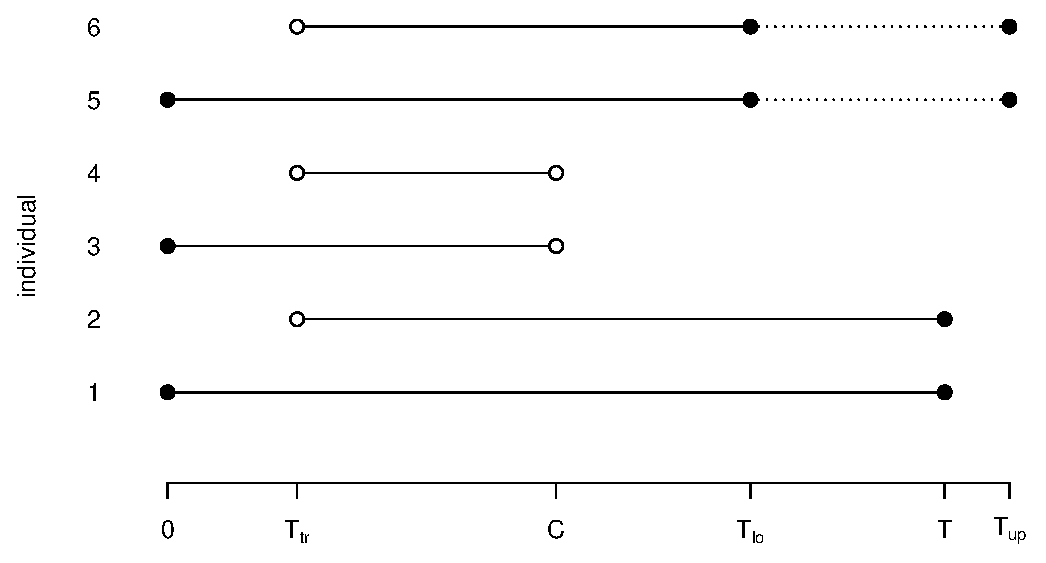
\epsfig{file=grafiken/censoringschemes.eps,scale=0.7}
{\it\caption{Illustration of different censoring
schemes.\label{censoringschemes}}}
\end{center}
\end{figure}

In a general framework an observation can now be uniquely described
 by the quadruple $(T_{tr},T_{lo},T_{up},\delta)$, with
\begin{center}
\begin{tabular}{ll}
$T_{lo}=T_{up}=T$, $\delta=1$ & if the observation is uncensored,\\
$T_{lo}=T_{up}=C$, $\delta=0$ & if the observation is right censored,\\
$T_{lo}<T_{up}$, $\delta=0$ & if the observation is interval censored.\\
\end{tabular}
\end{center}
For left truncated observations we have $T_{tr}>0$ while $T_{tr}=0$
for observations which are not truncated.

Based on these definitions we can now construct the likelihood
contributions for the different censoring schemes in terms of the
hazard rate $\lambda(t)$ and the survivor function
$S(t)=\exp(\int_0^t\lambda(u)du)$. Under the common assumption of
noninformative censoring and conditional independence, the
likelihood is given by
\begin{equation}\label{likelihood}
 L=\prod_{i=1}^n L_i,
\end{equation}
where
\[L_i = \lambda(T_{up})S(T_{up})/S(T_{tr}) = \lambda(T_{up})\exp\left(-\int_{T_{tr}}^{T_{up}}\lambda(t)dt\right)\]
for an uncensored observation,
\[L_i = S(T_{up})/S(T_{tr}) = \exp\left(-\int_{T_{tr}}^{T_{up}}\lambda(t)dt\right)\]
for a right censored observation and
\[L_i = (S(T_{lo})-S(T_{up}))/S(T_{tr}) = \exp\left(-\int_{T_{tr}}^{T_{lo}}\lambda(t)dt\right)\left(1-\exp\left(-\int_{T_{lo}}^{T_{up}}\lambda(t)dt\right)\right)\]
for an interval censored observation. Note that for explicit
evaluation of the likelihood (\ref{likelihood}) some numerical
integration technique has to be employed, since none of the
integrals can in general be solved analytically.

The above notation also allows for the easy inclusion of piecewise
constant, time-varying covariates via some data augmentation. Noting
that
\[\int_{T_{tr}}^{T}\lambda(t)dt = \int_{T_{tr}}^{t_1}\lambda(t)dt + \int_{t_1}^{t_2}\lambda(t)dt + \ldots + \int_{t_{p-1}}^{t_p}\lambda(t)dt + \int_{t_p}^{T}\lambda(t)dt\]
for $T_{tr}<t_1<\ldots<t_q<T$, we can replace an observation
$(T_{tr},T_{lo},T_{up},\delta)$ by a set of new observations
$(T_{tr},t_1,t_1,0)$, $(t_1,t_2,t_2,0)$, \ldots
$(t_{p-1},t_p,t_p,0)$, $(t_{p},T_{lo},T_{up},\delta)$ without
changing the likelihood. Therefore, observations with time-varying
covariates can be split up into several observations, where the
values $t_1<\ldots<t_p$ are defined by the changepoints of the
covariate and the covariate is now time-constant on each of the
intervals. In theory, other paths for a covariate $x(t)$ than
piecewise constant ones are also possible, if $x(t)$ is known for
$T_{tr}\le t\le T_{lo}$. In this case the the likelihood
(\ref{likelihood}) can also be evaluated numerically but a general
path $x(t)$ may lead to complicated data structures.

Figure \ref{timevaryingcovs} illustrates the data augmentation step
for a left truncated, uncensored observation and a covariate $x(t)$
that takes the three different values $x_1,x_2$ and $x_3$ on the
three intervals $[T_{tr},t_1], [t_1,t_2]$ and $[t_2,T_{up}]$. Here,
the original observation $(T_{tr},T_{up},T_{up},1)$ has to be
replaced by $(T_{tr},t_1,t_1,0)$, $(t_1,t_2,t_2,0)$ and
$(t_2,T_{up},T_{up},1)$.
\begin{figure}[htb]
\begin{center}
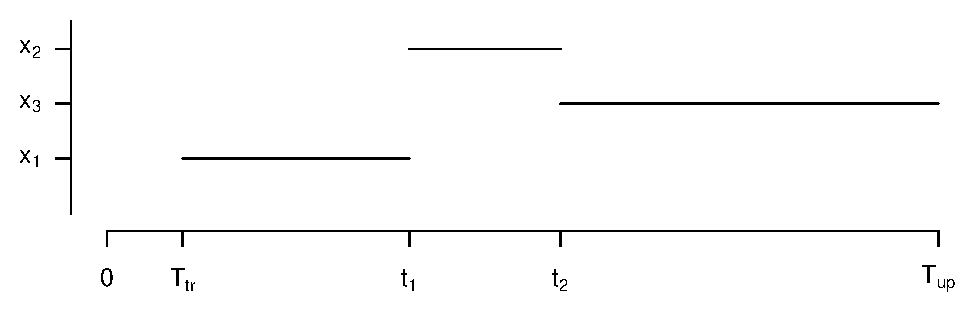
\epsfig{file=grafiken/timevaryingcovs.eps,scale=0.7}
{\it\caption{Illustration of time-varying
covariates.\label{timevaryingcovs}}}
\end{center}
\end{figure}

Currently, interval censored survival times can only be handled with
{\em remlreg objects}.

\subsection{Continuous-time multi-state models}\label{msmodels}
\index{Multi-state models}\index{Recurrent Events}\index{Disease
progression}\index{Competing risks}

Multi-state models are a flexible tool for the analysis of
time-continuous phenomena that can be characterized by a discrete
set of states. Such data structures naturally arise when observing a
discrete response variable for several individuals or objects over
time. Some common examples are depicted in Figure~\ref{some_msms} in
terms of their reachability graph for illustration. For recurrent
events (Figure~\ref{some_msms} (a)), the observations evolve through
time moving repeatedly between a fixed set of states. Other model
classes involve absorbing states, for example disease progression
models (Figure~\ref{some_msms} (b)), that are used to describe the
chronological development of a certain disease. If the severity of
this disease can be grouped into $q-1$ ordered stages of increasing
severity, a reasonable model might look like this: Starting from
disease state '$j$', an individual can only move to contiguous
states, i.e. either the disease gets worse and the individual moves
to state '$j+1$', or the disease attenuates and the individual moves
to state '$j-1$'. In addition, death is included as a further,
absorbing state '$q$', which can be reached from any of the disease
states. A model with several absorbing states is the competing risks
model (Figure~\ref{some_msms} (c)) where, for example, different
causes of death are analysed simultaneously.

\begin{figure}
\begin{center}
  \vspace{3mm}
 \mbox
 {
 \beginpicture
 \setcoordinatesystem units <0.65cm,0.65cm> point at 0 0
 \setlength{\unitlength}{0.65cm}

 \put {(a) Recurrent events} [Bl] at 0 16.5

 \put {\circle{1}} [Bl] at 7.5 12
 \put {\bf3} [Bl] at 7.35 11.85

 \put {\circle{1}} [Bl] at 5.5 14.5
 \put {\circle{1}} [Bl] at 9.5 14.5
 \put {\bf1} [Bl] at 5.35 14.35
 \put {\bf2} [Bl] at 9.35 14.35

 \arrow <3mm> [0.2,0.5] from 6.3 14.65 to 8.7 14.65
 \arrow <3mm> [0.2,0.5] from 8.7 14.35 to 6.3 14.35

 \arrow <3mm> [0.2,0.5] from  5.55 13.85 to 6.9 12.65
 \arrow <3mm> [0.2,0.5] from  7.25 12.65 to 5.9 13.85

 \arrow <3mm> [0.2,0.5] from  9.1 13.85 to 7.75 12.65
 \arrow <3mm> [0.2,0.5] from  8.1 12.65 to 9.45 13.85


 \put {(b) Disease progression} [Bl] at 0 10.5

 \put {\circle{1}} [Bl] at 7.5 6
 \put {$q$} [Bl] at 7.35 5.85

 \put {\circle{1}} [Bl] at 1.5 9
 \put {\circle{1}} [Bl] at 4.5 9
 \put {\circle{1}} [Bl] at 7.5 9
 \put {\circle{1}} [Bl] at 13.5 9
 \put {\bf1} [Bl] at 1.35 8.85
 \put {\bf2} [Bl] at 4.35 8.85
 \put {\bf3} [Bl] at 7.35 8.85
 \put {$q$-1} [Bl] at 13.15 8.85

 \put{$\cdots$} [Bl] at 10.1 8.9

 \arrow <3mm> [0.2,0.5] from 2.2 9.15 to 3.8 9.15
 \arrow <3mm> [0.2,0.5] from  3.8 8.85 to 2.2 8.85

 \arrow <3mm> [0.2,0.5] from 5.2 9.15 to 6.8 9.15
 \arrow <3mm> [0.2,0.5] from  6.8 8.85 to 5.2 8.85

 \arrow <3mm> [0.2,0.5] from 8.2 9.15 to 9.8 9.15
 \arrow <3mm> [0.2,0.5] from  9.8 8.85 to 8.2 8.85

 \arrow <3mm> [0.2,0.5] from 11.2 9.15 to 12.8 9.15
 \arrow <3mm> [0.2,0.5] from  12.8 8.85 to 11.2 8.85

 \arrow <3mm> [0.2,0.5] from  7.5 8.35 to 7.5 6.65
 \arrow <3mm> [0.2,0.5] from  4.75 8.35 to 7.0 6.65
 \arrow <3mm> [0.2,0.5] from  1.75 8.35 to 6.5 6.5
 \arrow <3mm> [0.2,0.5] from  13.25 8.35 to 8.5 6.5

 \put {(c) Competing risks} [Bl] at 0 4.5

 \put {\circle{1}} [Bl] at 1.5 0
 \put {\circle{1}} [Bl] at 4.5 0
 \put {\circle{1}} [Bl] at 7.5 0
 \put {\circle{1}} [Bl] at 13.5 0
 \put {\bf2} [Bl] at 1.35 -0.15
 \put {\bf3} [Bl] at 4.35 -0.15
 \put {\bf4} [Bl] at 7.35 -0.15
 \put {$q$} [Bl] at 13.35 -0.15

 \put {\circle{1}} [Bl] at 7.5 3
 \put {\bf1} [Bl] at 7.35 2.85

 \put{$\cdots$} [Bl] at 10.1 -0.1

 \arrow <3mm> [0.2,0.5] from  7.5 2.35 to 7.5 0.65

 \arrow <3mm> [0.2,0.5] from  6.9 2.6 to 4.75 0.65
 \arrow <3mm> [0.2,0.5] from  6.5 2.75 to 1.95 0.65
 \arrow <3mm> [0.2,0.5] from  8.5 2.75 to 12.85 0.65

 \endpicture
 }
 \vspace{3mm}

 \caption{Reachability graphs of some common multi-state
 models.\label{some_msms}}
\end{center}
\end{figure}

A multi-state model is fully described by a set of hazard rates
$\lambda_{hi}(t)$ where $h$, $h=1,\ldots,k$, indexes the type of the
transition and $i$, $i=1,\ldots,n$, indexes the individuals. Since
the hazard rates describe durations between transitions, we specify
them in analogy to hazard rate models for continuous time survival
analysis. To be more specific, $\lambda_{hi}(t)$ is modelled in a
multiplicative Cox-type way as
\[
 \lambda_{hi}(t) = \exp(\eta_{hi}(t)),
\]
where
\begin{equation}\label{addpred}
 \eta_{hi}(t) = g_{h0}(t) + \sum_{l=1}^Lg_{hl}(t)u_{il}(t) +
 \sum_{j=1}^Jf_{hj}(x_{ij}(t)) + v_i(t)'\gamma_h +  b_{hi}
\end{equation}
is an additive predictor consisting of the following components:
\begin{itemize}
 \item A time-varying, nonparametric baseline effect $g_{h0}(t)$ common for all
 observations.
 \item Covariates $u_{il}(t)$ with time-varying effects $g_{hl}(t)$.
 \item Nonparametric effects $f_{hj}(x_{ij}(t))$ of continuous covariates
 $x_{ij}(t)$.
 \item Parametric effects $\gamma_h$ of covariates $v_i(t)$.
 \item Frailty terms $b_{hi}$ to account for unobserved
 heterogeneity.
\end{itemize}

For each individual $i$, $i=1,\ldots,n,$ the likelihood contribution
in a multi-state model can be derived from a counting process
representation of the multi-state model. Let $N_{hi}(t)$,
$h=1,\ldots,k$ be a set of counting processes counting transitions
of type $h$ for individual $i$. Consequently, $h=1,\ldots,k$ indexes
the observable transitions in the model under consideration and the
jumps of the counting processes $N_{hi}(t)$ are defined by the
transition times of the corresponding multi-state process for
individual $i$.

From classical counting process theory (see e.g. \citeasnoun{Andetal93}, Ch.~VII.2), the intensity processes $\alpha_{hi}(t)$
of the counting processes $N_{hi}(t)$ are defined as the product of the hazard rate for type $h$ transitions $ \lambda_{hi}(t)$
and a predictable at-risk indicator process $Y_{hi}(t)$, i.e.
\[
 \alpha_{hi}(t) = Y_{hi}(t) \lambda_{hi}(t),
\]
where the hazard rates are constructed in terms of covariates as in
(\ref{addpred}). The at-risk indicator $Y_{hi}(t)$ takes the value
one if individual $i$ is at risk for a type $h$ transition at time
$t$ and zero otherwise. For example, in the multi-state model of
Figure~\ref{some_msms}a), an individual in state 2 is at risk for
both transitions to state 1 and state 3. Hence, the at-risk
indicators for both the transitions '2 to 1' and '2 to 3' will be
equal to one as long as the individual remains in state 2.

Under mild regularity conditions, the individual log-likelihood
contributions can now be obtained from counting process theory as
\begin{equation}\label{loglike1}
 l_i = \sum_{h=1}^k\left[ \int_0^{T_i}\log(\lambda_{hi}(t))dN_{hi}(t) -
 \int_0^{T_i}\lambda_{hi}(t)Y_{hi}(t)dt\right],
\end{equation}
where $T_i$ denotes the time until which individual $i$ has been
observed. The likelihood contributions can be interpreted similarly
as with hazard rate models for survival times (and in fact coincide
with these in the case of a multi-state process with only one
transition to an absorbing state). The first term corresponds to
contributions at the transition times since the integral with
respect to the counting process in fact equals a simple sum over the
transition times. Each of the summands is then given by the
log-intensity for the observed transition evaluated at this
particular time point. In survival models this term simply equals
the log-hazard evaluated at the survival time for uncensored
observations. The second term reflects cumulative intensities
integrated over accordant waiting periods between two successive
transitions. The integral is evaluated for all transitions the
corresponding person is at risk at during the current period. In
survival models there is only one such transition (the transition
from 'alive' to 'dead') and the integral is evaluated from the time
of entrance to the study to the survival or censoring time.

More details on multi-state models, including an exemplary analysis on human sleep, can be found in \citeasnoun{KneHen06}.

\addcontentsline{toc}{section}{Bibliography}

\begin{thebibliography}{99}

\harvarditem{Albert \& Chib}{1993}{AlbChi93}
 {\scshape Albert, J. \& Chib, S.} (1993).
 Bayesian analysis of binary and polychotomous response data.
 {\it Journal of the American Statistical Association}, {\bf 88}, 669--679.

\harvarditem{Andersen et al.}{1993}{Andetal93}
 {\scshape Andersen, P. K., Borgan, {\O}, Gill, R. D. \& Keiding, N.} (1993).
 {\it Statistical Models Based on Counting Processes.}
 New York: Springer Verlag.

\harvarditem{Andrews \& Mallows}{1974}{AndMal74}
 {\scshape Andrews, D. F. \& Mallows, C. L.} (1974).
 Scale mixtures of normal distributions.
 {\it Journal of the Royal Statistical Society B}, {\bf 36}, 99--102.

\harvarditem{Bollaerts, Eilers \& van Mechelen}{2006}{BolEilvMe06}
 {\scshape Albert, J. \& Chib, S.} (1993).
 Simple and Multiple P-Spline Regression with Shape Constraints.
 {\it British Journal of Mathematical and Statistical Psychology}, {\bf 59}, 451--469.

\harvarditem{Belitz}{2007}{Bel07}
 {\scshape Belitz, C.} (2007).
 {\it Model Selection in Generalized Structured Additive Regression Models.}
 PhD Thesis, University of Munich.

\harvarditem{Belitz \& Lang}{2008}{BelLan08}
{\scshape Belitz, C. \& Lang, S.} (2008).
 Simultaneous selection of variables and smoothing parameters in structured additive regression models.
{\it Computational Statistics and Data Analysis}, {\bf 53} , 61-81.

\harvarditem{Besag, York \& Molli\'{e}}{1991}{BesYorMol91}
 {\scshape Besag, J., York, J. \& Molli\'{e}, A.} (1991).
 Bayesian image restoration with two applications in spatial statistics (with discussion).
 {\it Annals of the Institute of Statistical Mathematics}, {\bf 43}, 1--59.

\harvarditem{Brezger \& Lang}{2006}{BreLan06}
 {\scshape Brezger, A. \& Lang, S.} (2006).
 Generalized additive regression based on Bayesian P-splines.
 {\it Computational Statistics and Data Analysis} {\bf 50}, 967--991.

\harvarditem{Devroye}{1986}{Dev86}
 {\scshape Devroye, L.} (1986).
 {\it Non-Uniform Random Variate Generation.}
 New York: Springer Verlag.

\harvarditem{Eilers \& Marx}{1996}{EilMar96}
 {\scshape Eilers, P. H. C. \& Marx, B. D.} (1996).
 Flexible smoothing using B-splines and penalized likelihood (with comments and rejoinder).
 {\it Statistical Science}, {\bf 11}, 89--121.

\harvarditem{Fahrmeir, Kneib \& Lang}{2004}{FahKneLan04}
 {\scshape Fahrmeir, L., Kneib, T. \& Lang, S.} (2004).
 Penalized structured additive regression for space-time data: A Bayesian perspective.
 {\it Statistica Sinica}, {\bf 14}, 715--745.

\harvarditem{Fahrmeir \& Lang}{2001}{FahLan01a}
 {\scshape Fahrmeir, L. \& Lang, S.} (2001a).
 Bayesian Inference for Generalized Additive Mixed Models Based on Markov Random Field Priors.
 {\it Journal of the Royal Statistical Society C}, {\bf 50}, 201--220.

\harvarditem{Fahrmeir \& Lang}{2001}{FahLan01b}
 {\scshape Fahrmeir, L. \& Lang, S.} (2001b).
 Bayesian Semiparametric Regression Analysis of Multicategorical Time-Space Data.
 {\it Annals of the Institute of Statistical Mathematics}, {\bf 53}, 10--30.

\harvarditem{Fahrmeir \& Osuna}{2006}{FahOsu06}
 {\scshape Fahrmeir, L. \& Osuna, L.} (2006).
 Structured additive regression for overdispersed and zero-inflated count data.
 {\it Applied Stochastic Models in Business and Industry}, {\bf 22}, 351--369

 \harvarditem{Fahrmeir \& Tutz}{2001}{FahTut01}
 {\scshape Fahrmeir, L. \& Tutz, G.} (2001).
 {\it Multivariate Statistical Modelling based on Generalized Linear Models.}
 New York: Springer-Verlag.

\harvarditem{Fotheringham, Brunsdon \& Charlton}{2002}{FotBruCha02}
 {\scshape Fotheringham, A. S., Brunsdon, C., \& Charlton, M. E.} (2002).
 {\it Geographically Weighted Regression: The Analysis of Spatially Varying Relationships.}
 Chichester: Wiley.

\harvarditem{Gamerman}{1997}{Gam97}
 {\scshape Gamerman, D.} (1997).
 Efficient Sampling from the posterior distribution in generalized linear models.
 {\it Statistics and Computing}, {\bf 7}, 57--68.

\harvarditem{Gelfand, Sahu \& Carlin}{1996}{GelSahCar96}
 {\scshape Gelfand, A. E., Sahu, S. K. \& Carlin, B. P.} (1996).
 Efficient Parametrizations for Genera\-lized Linear Mixed Models.
 In: Bernardo, J. M., Berger, J. O., Dawid, A. P. \& Smith, A. F. M. (eds.),
 {\it Bayesian Statistics 5}, 165--180.
 Oxford University Press.

\harvarditem{George \& Liu}{1981}{GeoLiu81}
 {\scshape George, A. \& Liu, J.W.} (1981).
 {\it Computer Solution of Large Sparse Positive Definite Systems.}
 Series in computational mathematics, Prentice-Hall.

\harvarditem{Green}{1987}{Gre87}
 {\scshape Green, P. J.} (1987).
 Penalized likelihood for general semiparametric regression models.
 {\it International Statistical Review}, {\bf 55}, 245--259.

\harvarditem{Green}{2001}{Gre01}
 {\scshape Green, P. J.} (2001).
 A Primer in Markov Chain Monte Carlo.
 In: Barndorff-Nielsen, O. E., Cox, D. R. \& Kl\"{u}ppelberg, C. (eds.),
 {\it Complex Stochastic Systems}, 1--62.
 Chapmann and Hall, London.

\harvarditem{Green \& Silverman}{1994}{GreSil94}
 {\scshape Green, P. J. \& Silverman, B.} (1994).
 {\it Nonparametric Regression and Generalized Linear Models.}
 Chapman and Hall, London.

\harvarditem{Griffin \& Brown}{2005}{GriBro05}
 {\scshape Griffin, J. E., and Brown, P. J.} (2005). Alternative prior distributions
 for variable selection with very many more variables than observations. Technical
 report, University of Warwick, Dept. of Statistics.

\harvarditem{Harville}{1977}{Har77}
 {\scshape Harville, D. A.} (1977).
 Maximum Likelihood approaches to variance component estimation and to related problems.
 {\it Journal of the American Statistical Association}, {\bf 72}, 320--338.

\harvarditem{Hastie \& Tibshirani}{1990}{HasTib90}
 {\scshape Hastie, T. \& Tibshirani, R.} (1990).
 {\it Generalized additive models.}
 Chapman and Hall, London.

\harvarditem{Hastie \& Tibshirani}{1993}{HasTib93}
 {\scshape Hastie, T. \& Tibshirani, R.} (1993).
 Varying-coefficient Models.
 {\it Journal of the Royal Statistical Society B}, {\bf 55}, 757--796.

\harvarditem{Hastie \& Tibshirani}{2000}{HasTib00}
 {\scshape Hastie, T. \& Tibshirani, R.} (2000).
 Bayesian Backfitting.
 {\it Statistical Science}, {\bf 15}, 193--223.

\harvarditem{Hastie, Tibshirani \& Firedman}{2001}{HasTibFri01}
 {\scshape Hastie, T., Tisbshirani, R. \& Friedman, J.} (2001).
 {\it The Elements of Statistical Learning: Data Mining, Inference and Prediction.}
 New York: Springer-Verlag.

\harvarditem{Hennerfeind, Brezger \& Fahrmeir}{2006}{HenBreFah06}
 {\scshape Hennerfeind, A., Brezger, A. \& Fahrmeir, L.} (2006).
 Geoadditive survival models.
 {\it Journal of the American Statistical Association}, {\bf 101}, 1065--1075.

\harvarditem{Holmes \& Held}{2006}{HolHel06}
 {\scshape Holmes, C., Held, L.} (2006).
 Bayesian auxiliary variable models for binary and multinomial regression.
 {\it Bayesian Analysis}, {\bf 1}, 145--168.

\harvarditem{Hurvich, Simonoff \& Tsai}{1998}{HurSimTsa98}
 {\scshape Hurvich, C. M., Simonoff, J. S. \& Tsai, C. L.} (1998).
 Smoothing parameter selection in nonparametric regression using an improved {A}kaike information criterion.
 {\it Journal of the Royal Statistical Society B}, {\bf 60}, 271--293.

\harvarditem{Ishwaran \& Rao}{2005}{IshRao05}
 {\scshape Ishwaran, H., and Rao, S. J.} (2005). Spike and Slab Variable
 Selection: Frequentist and Bayesian Strategies. {\it The Annals of Statistics},
 {\bf 33}, 730-773.

\harvarditem{Johnson, Moore \& Ylvisaker}{1990}{JohMooYlv90}
 {\scshape Johnson, M.E., Moore, L.M. \& Ylvisaker, D.} (1990).
 Minimax and maximin designs.
 {\it Journal of Statistical Planning and Inference}, {\bf 26}, 131--148.

\harvarditem{Kammann \& Wand}{2003}{KamWan03}
 {\scshape Kammann, E. E. \& Wand, M. P.} (2003).
 Geoadditive Models.
 {\it Journal of the Royal Statistical Society C}, {\bf 52}, 1--18.

\harvarditem{Kneib}{2006}{Kne06}
 {\scshape Kneib, T.} (2006).
 Geoadditive hazard regression for interval censored survival times.
 {\it Computational Statistics and Data Analysis}, {\bf 51}, 777--792

\harvarditem{Kneib \& Hennerfeind}{2006}{KneHen06}
 {\scshape Kneib, T. \& Hennerfeind, A.} (2006).
 Bayesian Semiparametric Multi-State Models.
 {\it Statistical Modelling}, {\bf 8}, 169--198.

\harvarditem{Kneib \& Fahrmeir}{2006}{KneFah06}
 {\scshape Kneib, T. \& Fahrmeir, L.} (2006).
 Structured additive regression for categorical space-time data: A mixed model approach.
 {\it Biometrics}, {\bf 62}, 109--118.

\harvarditem{Kneib \& Fahrmeir}{2007}{KneFah07}
 {\scshape Kneib, T. \& Fahrmeir, L.} (2007).
 A mixed model approach to structured hazard regression.
 {\it Scandinavian Journal of Statistics}, {\bf 34}, 207--228.

\harvarditem{Kneib et al.}{2009}{Kne09}
 {\scshape Kneib, T., Konrath, S. und Fahrmeir, L.} (2009). High-dimensional
 Structured Additive Regression Models: Bayesian Regularisation, Smoothing and Predictive
 Performance. Department of Statistics, Technical Report No. 46, LMU Munich.

\harvarditem{Knorr-Held}{1999}{KnoHel99}
 {\scshape Knorr-Held, L.} (1999).
 Conditional Prior Proposals in Dynamic Models.
 {\it Scandinavian Journal of Statistics}, {\bf 26}, 129--144.

\harvarditem{Konrath et al.}{2008}{Kon08}
 {\scshape Konrath, S., Kneib, T., Fahrmeir, L.} (2008). Bayesian Regularisation
 in Structured Additive Regression Models for Survival Data. Department of Statistics,
 Technical Report No.35, LMU Munich.

\harvarditem{Lang \& Brezger}{2004}{LanBre04}
 {\scshape Lang, S. \& Brezger, A.} (2004).
 Bayesian P-splines.
 {\it Journal of Computational and Graphical Statistics}, {\bf 13}, 183--212.

\harvarditem{Lin \& Zhang}{1999}{LinZha99}
 {\scshape Lin, X. \& Zhang, D.} (1999).
 Inference in generalized additive mixed models by using smoothing splines.
 {\it Journal of the Royal Statistical Society B}, {\bf 61}, 381--400.

\harvarditem{McCullagh \& Nelder}{1989}{McCNel89}
 {\scshape McCullagh, P. \& Nelder, J. A.} (1989).
 {\it Generalized Linear Models.}
 Chapman and Hall, London.

\harvarditem{M\"{u}ller, Stadtm\"{u}ller \& Tabnak}{1997}{MueStaTab97}
 {\scshape M\"{u}ller, H. G., Stadtm\"{u}ller, U. \& Tabnak, F.} (1997).
 Spatial Smoothing of Geographically Aggregated Data, with Applications to the Construction of Incidence Maps.
 {\it Journal of the American Statistical Association} {\bf 92}, 61--71.

\harvarditem{Nychka \& Saltzman}{1998}{NycSal98}
 {\scshape Nychka, D. \& Saltzman, N.} (1998).
 {\it Design of Air-Quality Monitoring Networks.}
 Lecture Notes in Statistics, 132, 51--76.

\harvarditem{Osuna}{2004}{Osu04}
 {\scshape Osuna, L.} (2004)
 {\it Semiparametric Bayesian Count Data Models}.
 Dr. Hut Verlag, M\"{u}nchen.

\harvarditem{Park \& Casella}{2008}{ParCas08}
 {\scshape Park, T., and Casella, G.} (2008). The Bayesian Lasso.
 {\it Journal of the American Statistical Association}, {\bf 482}, 681-686.

\harvarditem{Rue}{2001}{Rue01}
 {\scshape Rue, H.} (2001).
 Fast Sampling of Gaussian Markov Random Fields with Applications.
 {\it Journal of the Royal Statistical Society B}, {\bf 63}, 325--338.

\harvarditem{Ruppert, Wand \& Carroll}{2003}{RupWanCar03}
 {\scshape Ruppert, D., Wand, M. P. \& Carroll, R. J.} (2003).
 {\it Semiparametric Regression.}
 Cambridge University Press.

\harvarditem{Spiegelhalter et al.}{2002}{SpiBesCar02}
 {\scshape Spiegelhalter, D. J., Best, N. G., Carlin, B. P. \& van der Linde, A.} (2002).
 Bayesian measures of model complexity and fit.
 {\it Journal of the Royal Statistical Society B}, {\bf 65}, 583--639.

\end{thebibliography}

\addcontentsline{toc}{section}{Index}
\documentclass[11pt,a4paper,twoside]{bayesxarticle}


\usepackage{amsfonts}
\usepackage[dvips]{graphicx}
\usepackage[dvips]{epsfig}
\usepackage{fancyhdr}
\usepackage{dsfont}
\usepackage{amsmath}
\usepackage{dsfont}
\usepackage{amssymb}

%\usepackage{showkeys}
%\usepackage{showidx}

\usepackage{rotating}
\usepackage{shortvrb}
\usepackage{multicol}
\usepackage{longtable}
\usepackage{xr}

\usepackage[ps2pdf]{thumbpdf}
\usepackage[ps2pdf]{hyperref}

\input{prepictex}
\input{pictexwd}
\input{postpictex}

\hypersetup{
%    pdffitwindow=true,
    pdfstartview=FitB,
    pdftitle={BayesX Manuals},
    pdfauthor={Christiane Belitz, Andreas Brezger, Thomas Kneib, Stefan Lang and Nikolaus Umlauf},
    colorlinks=true,
    linkcolor=blue,
    pdfpagemode=UseOutlines,
    bookmarksopen=true,
    bookmarksnumbered=true,
    pdfstartpage={1},
    hyperindex=true
    }

\usepackage[dcu]{harvard}

\sloppy
\parindent0em
\parskip0.3em
\topmargin -0.3cm \textheight24cm \textwidth16.5cm \headheight0.5cm \oddsidemargin-0.4cm \evensidemargin-0.4cm

 \fancyhead[RO,LE]{\thepage}
 \fancyhead[C]{}
 \fancyhead[LO]{\nouppercase\rightmark}
 \fancyhead[RE]{\nouppercase\leftmark}
 \fancyfoot[RO,LE]{}
 \fancyfoot[C]{\small\today} %Am ende raus!!!
 \fancyfoot[LO,RE]{}
 \fancyfoot[C]{}

 \renewcommand{\headrulewidth}{.4pt}
 \renewcommand{\footrulewidth}{0pt} %Am Ende 0 !!!

\pagestyle{fancy}


\renewcommand{\descriptionlabel}[1]{\hspace\labelsep\sc #1}

 \newcommand{\Cov}{\mbox{Cov}}
 \newcommand{\diag}{\mbox{diag}}
 \newcommand{\trace}{\mbox{trace}}
 \newcommand{\df}{\mbox{df}}

\def \re {{\bf R}}
\def \beq {\begin{equation}}
\def \eeq {\end{equation}}
\def \bdis {\begin{displaymath}}
\def \edis {\end{displaymath}}
\def \ds {\displaystyle}

\def \mbeta {\mbox{\boldmath $\beta$}}
\def \mtheta {\mbox{\boldmath $\theta$}}
\def \hatmbeta {\mbox{\boldmath $\hat\beta$}}
\def \eps {\epsilon}
\def \meps {\mbox{\boldmath $\epsilon$}}
\def \mmu {\mbox{\boldmath $\mu$}}
\def \mnu {\mbox{\boldmath $\nu$}}
\def \mSigma {\mbox{\boldmath $\Sigma$}}
\def \mGamma {\mbox{\boldmath $\Gamma$}}
\def \msigma {\mbox{\boldmath $\sigma$}}
\def \mPhi {\mbox{\boldmath $\Phi$}}
\def \Sigmavec {\mbox{\boldmath $\Sigma$}}
\def \sigmavec {\mbox{\boldmath $\sigma$}}
\def \nuvec {\mbox{\boldmath $\nu$}}
\def \tauvec {\mbox{\boldmath $\tau$}}




\newcommand{\N}{\mbox{N}}
\newcommand{\Var}{\mbox{Var}}
\newcommand{\E}{\mbox{E}}

\newcommand{\X}{\mbox{\boldmath $X$}}
\newcommand{\x}{\xvec}
\newcommand{\Z}{\mbox{\boldmath $Z$}}
\newcommand{\z}{\mbox{\boldmath $z$}}
\newcommand{\mb}{\mbox{\boldmath $b$}}
\newcommand{\Fx}{\mbox{\scriptsize \boldmath $x$}}
\newcommand{\I}{\mbox{\boldmath $I$}}
\newcommand{\Y}{\mbox{\boldmath $Y$}}
\newcommand{\y}{\mbox{\boldmath $y$}}
\newcommand{\mS}{\mbox{\boldmath $S$}}
\newcommand{\T}{\mbox{\boldmath $T$}}
\newcommand{\K}{\mbox{\boldmath $K$}}
\newcommand{\kt}{\mbox{\boldmath $t$}}
\newcommand{\U}{\mbox{\boldmath $U$}}
\newcommand{\fu}{\mbox{\boldmath $u$}}
\newcommand{\ba}{\mbox{\boldmath $\alpha$}}
\newcommand{\bb}{\mbox{\boldmath $\beta$}}

\def \Mvec {\vec{M}}
\def \Kvec {\vec{K}}
\def \mM {\vec{M}}
\def \Pvec {\vec{P}}
\def \Svec {\vec{S}}
\def \deltavec {\vec{\delta}}
\def \lambdavec {\boldsymbol{\lambda}}
\def \Lambdavec {\boldsymbol{\Lambda}}
\def \betavec {\boldsymbol{\beta}}
\def \etavec {\boldsymbol{\eta}}
\def \gammavec {\boldsymbol{\gamma}}
\def \Gammavec {\boldsymbol{\Gamma}}
\def \Omegavec {\boldsymbol{\Omega}}
\def \muvec {\boldsymbol{\mu}}
\def \kappavec {\boldsymbol{\kappa}}
\def \nuvec {\boldsymbol{\nu}}
\def \pivec {\vec{\pi}}
\def \thetavec {\vec{\theta}}
\def \varthetavec{\vec{\vartheta}}
\def \varepsilonvec {\boldsymbol{\varepsilon}}
\def \zetavec {\vec{\zeta}}
\def \Sigmavec {\boldsymbol{\Sigma}}
\def \Thetavec {\boldsymbol{\theta}}

\def \dvec {\mathbf{d}}
\def \fvec {\mathbf{f}}
\def \fhatvec {\mathbf{\hat{f}}}
\def \svec {\mathbf{s}}
\def \wvec {\mathbf{w}}
\def \xvec {\mathbf{x}}
\def \yvec {\mathbf{y}}
\def \uvec {\mathbf{u}}
\def \avec {\mathbf{a}}
\def \zvec {\mathbf{z}}
\def \bvec {\mathbf{b}}
\def \tvec {\mathbf{t}}
\def \mvec {\mathbf{m}}
\def \cvec {\mathbf{c}}

\def \ds {\displaystyle}

\def \Gvec {\mathbf{G}}
\def \Rvec {\mathbf{R}}
\def \Avec {\mathbf{A}}
\def \Bvec {\mathbf{B}}
\def \Cvec {\mathbf{C}}
\def \Dvec {\mathbf{D}}
\def \Fvec {\mathbf{F}}
\def \Kvec {\mathbf{K}}
\def \Hvec {\mathbf{H}}
\def \Ivec {\mathbf{I}}
\def \Lvec {\mathbf{L}}
\def \Uvec {\mathbf{U}}
\def \Wvec {\mathbf{W}}
\def \Yvec {\mathbf{Y}}
\def \Zvec {\mathbf{Z}}
\def \svec {\mathbf{s}}
\def \Cvec {\mathbf{C}}
\def \dvec {\mathbf{d}}
\def \Avec {\mathbf{A}}
\def \Pvec {\mathbf{P}}
\def \Vvec {\mathbf{V}}
\def \xivec {\mathbf{x_i}}
\def \xjvec {\mathbf{x_j}}
\def \betavecr {\vec{\beta_r}}
\def \betavec {\boldsymbol{\beta}}
\def \betadach {\hat{\vec{\beta}}}
\def \betadachr {\vec{\hat{\beta}_r}}
\def \betaschl {\vec{\tilde{\beta}}}
\def \betaschlr {\vec{\tilde{\beta}_r}}
\def \sschlr {\vec{\tilde{s}_r}}
\def \Aschlr {\vec{\tilde{A}_r}}
\def \Adach {\vec{\hat{A}}}
\def \Avecr {\vec{A}_r}
\def \Adachr {\vec{\hat{A}_r}}
\def \Fdach {\vec{\hat{F}}}
\def \Vdach {\vec{\hat{V}}}
\def \Aschl {\vec{\tilde{A}}}
\def \Xvec {\mathbf{X}}

\def \nullvec {\boldsymbol{0}}

\def \hvec {\vec{h}}
\def \vvec {\vec{v}}
\def \wvec {\vec{w}}
\def \x1vec {\vec{x_1}}
\def \xnvec {\vec{x_n}}

\def \Kmat {\mathbf{K}}
\def \Kmatj {\mathbf{K}_j}
\def \Xmat {\mathbf{X}}
\def \Vmat {\mathbf{V}}
\def \Smat {\mathbf{S}}


\def \dsR {\text{$\mathds{R}$}}
 \DeclareMathOperator{\B}{B}

\def \einsvec {\boldsymbol{1}}

\newcommand{\subheader}[1]{\textsf{\textbf{{\large #1}}}}

\newenvironment{stanza}[2]{\subheader{#1} \begin{itemize} \item[]#2}{\end{itemize}}


\newcommand{\preface}[1]{
\thispagestyle{empty}

\begin{center}
{\bf \em \huge BayesX}

\vspace{0.5cm}

{\em \large Software for Bayesian Inference in Structured Additive Regression Models}

\vspace{0.5cm}

{\em Version 2.1}

\vspace{0.5cm}

\begin{figure}[h]
\begin{center}
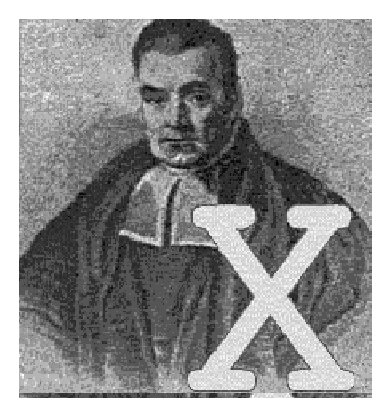
\includegraphics[scale=1.2]{grafiken/bayesicon.eps}
\end{center}
\end{figure}

\vfill

{\bf\sffamily \huge #1}

\vfill

\end{center}

{\em Developed by}

Christiane Belitz\\
Andreas Brezger\\
Thomas Kneib (University of G{\"o}ttingen)\\
Stefan Lang (University of Innsbruck) \\
Nikolaus Umlauf (University of Innsbruck) \\

\vspace{2ex}

{\em With contributions by}

\vspace{-1.5ex}

\begin{multicols}{2}
Daniel Adler
Eva-Maria Fronk\\
Felix Heinzl\\
Andrea Hennerfeind\\
Manuela Hummel\\
Alexander Jerak\\
Susanne Konrath\\
Petra Kragler\\
Cornelia Oberhauser\\
Leyre Est\'{\i}baliz Osuna Echavarr\'{\i}a\\
Daniel Saban\'{e}s Bov\'{e} \\
Achim Zeileis
\end{multicols}

{\em Supported by}

Ludwig Fahrmeir (mentally)\\
Leo Held (mentally)\\
German Research Foundation (DFG)

\newpage

\subsection*{Acknowledgements}

The development of {\em BayesX} has been supported by grants from the German Research Foundation (DFG), Collaborative
Research Center 386 ``Statistical Analysis of Discrete Structures''.

Special thanks go to (in alphabetical order of first names):

{\em Dieter Gollnow} for computing and providing the map of Munich (a really hard job); \\
{\em Leo Held} for advertising the program; \\
{\em Ludwig Fahrmeir} for his patience with finishing the program and for carefully
reading and correcting the  manual; \\
{\em Ngianga-Bakwin Kandala} for being the first user of the program (a really hard job); \\
{\em Samson Babatunde Adebayo} for carefully reading and correcting the manual; \\
{\em Ursula Becker} for carefully reading and correcting the manual;

\subsection*{Licensing agreement}

This program is free software; you can redistribute it and/or
modify it under the terms of the GNU General Public License
as published by the Free Software Foundation; either version 2
of the License, or (at your option) any later version.

This program is distributed in the hope that it will be useful,
but WITHOUT ANY WARRANTY; without even the implied warranty of
MERCHANTABILITY or FITNESS FOR A PARTICULAR PURPOSE.  See the
GNU General Public License for more details.

You should have received a copy of the GNU General Public License
along with this program; if not, write to the Free Software
Foundation, Inc., 51 Franklin Street, Fifth Floor, Boston, MA  02110-1301, USA.



\vspace{0.5cm}

{\em BayesX} is available at { \href{http://www.bayesx.org}{http://www.bayesx.org}}}


 \externaldocument{manual}
 \externaldocument{manual_tutorials}

 \makeindex

\begin{document}
\MakeShortVerb{\#}

\preface{Methodology Manual}

\newpage

\section{Introduction}

In this manual we provide a brief review of the methodological background for the three regression tools currently implemented
in {\em BayesX}. The first regression tool ({\em bayesreg objects}) relies on Markov chain Monte Carlo (MCMC) simulation
techniques and yields fully Bayesian posterior mean or posterior mode estimates. The second regression tool ({\em remlreg
objects}) is based on the mixed model representation of penalised regression models with inference being based on penalised
maximum likelihood and marginal likelihood (a generalisation of restricted maximum likelihood) estimation. The third regression
tool ({\em stepwisereg objects}) simultaneously performs model choice and estimation with inference being based on penalised
likelihood. MCMC techniques are partly used for computing interval estimates. All regression tools allow to estimate structured
additive regression (STAR) models (\citeasnoun{BelLan08}, \citeasnoun{BreLan06}, \citeasnoun{FahKneLan04}) with complex semiparametric predictors.
STAR models cover a number of well
known model classes as special cases, including {\em generalized additive models} \cite{HasTib90}, {\em generalized additive
mixed models} \cite{LinZha99}, {\em geoadditive models} \cite{KamWan03}, {\em varying coefficient models}\cite{HasTib93}, and
{\em geographically weighted regression} \citeasnoun{FotBruCha02}. Besides models for responses from univariate exponential
families, BayesX also supports non-standard regression situations such as models for categorical responses with either ordered
or unordered categories, continuous time survival data, or continuous time multi-state models. To provide a first impression of
structured additive regression, Sections~\ref{obsmodel} to \ref{inference} describe STAR models for exponential family
regression. Section~\ref{survivalAnalysis} extends structured additive regression to the analysis of survival times and
multi-state data. Full details on STAR methodology can be found in the following references:

\subsubsection*{Structured additive regression based on MCMC
simulation}

\begin{itemize}
\item Brezger, A., Lang, S. (2006): Generalized structured additive regression based on Bayesian P-Splines. {\it
    Computational Statistics and Data Analysis}, {\bf 50}, 967--991.
    \vspace{-0.25cm}
\item Brezger, A., Lang, S. (2008)
      Simultaneous Probability statements for Bayesian P-splines.
      {\it Statistical Modelling}, {\bf 8},
      141--168.\vspace{-0.25cm}
\item Brezger, A., Steiner, W. (2008)
Monotonic regression based on Bayesian P-splines: an
application to estimating price response functions from
store-level scanner data. {\it Journal of Economic and Business Statistics}, {\bf 26}, 90--104.
\vspace{-0.25cm}
\item Fahrmeir, L., Lang, S. (2001): Bayesian Inference for Generalized Additive Mixed Models Based on Markov Random Field
    Priors. {\it Journal of the Royal Statistical Society C (Applied Statistics)}, {\bf 50}, 201--220.\vspace{-0.25cm}
\item Fahrmeir, L., Lang, S. (2001): Bayesian Semiparametric Regression Analysis of Multicategorical Time-Space Data. {\it
    Annals of the Institute of Statistical Mathematics}, {\bf 53}, 10--30.\vspace{-0.25cm}
\item Fahrmeir, L., Osuna, L.. (2006): Structured additive regression for overdispersed and zero-inflated count data. {\it
    Applied Stochastic Models in Business and Industry}, {\bf 22}, 351--369.\vspace{-0.25cm}
\item Hennerfeind, A., Brezger, A., Fahrmeir, L. (2006): Geoadditive survival models. {\it Journal of the American
    Statistical Association}, {\bf 101}, 1065--1075.\vspace{-0.25cm}
\item Kneib, T., Hennerfeind, A. (2006) Bayesian Semiparametric Multi-State Models. {\it Statistical Modelling}, {\bf 8},
    169--198..\vspace{-0.25cm}
\item Lang, S., Brezger, A. (2004): Bayesian P-Splines {\it Journal of Computational and Graphical Statistics}, {\bf 13},
    183--212.
\end{itemize}

Presumably the best starting point is the paper by \citeasnoun{BreLan06}.

\begin{figure}[ht]
\footnotesize
\begin{center}
%\begin{tabular}{|p{8cm}|p{5cm}|}
%\hline
%{\bf Intended use} & {\bf recommended sections } \\
%\hline
%semiparametric regression, fully Bayesian approach  & sections \ref{obsmodel}, \ref{priorassumptions} , \ref{fullbayes} \\
%\hline
%semiparametric regression, inference based on mixed model technology, classical perspective &
%sections \ref{obsmodel}, \ref{penalizedleastsquares}, \ref{glmmrep}, \ref{glmmmeth} \\
%\hline
%semiparametric regression, inference based on mixed model technology, Bayesian point of view & sections \ref{obsmodel}, \ref{priorassumptions},
%\ref{glmmrep}, \ref{glmmmeth} \\
%\hline
%semiparametric regression including model choice & sections \ref{obsmodel}, \ref{penalizedleastsquares}, \ref{stepwiseest} \\
%\hline
%\end{tabular}
% \vspace{3mm}
\[\mbox{
 \beginpicture
 \setcoordinatesystem units <1.1cm,1.1cm> point at 0 0
 \setlength{\unitlength}{1.1cm}

 \put {\framebox(5.5,0.7){\sffamily\bfseries 2 Generalized regression models}} at 0 0

 \put {Bayesian perspective} at -4 -1.2
 \put {frequentist perspective} at 4 -1.2

 \arrow <4mm> [0.25,0.75] <0pt,5mm> from 0 -1 to -5 -2.9
 \arrow <4mm> [0.25,0.75] <0pt,5mm> from 0 -1 to 5 -2.9

 \put {\framebox(4.5,0.7){\sffamily\bfseries 4 Bayesian point of view}} at -5 -3

 \put {\framebox(4.5,0.7){\sffamily\bfseries 3 Penalised likelihood}} at 5 -3

 \arrow <4mm> [0.25,0.75] <0pt,5mm> from -5 -4 to 0 -6
 \arrow <4mm> [0.25,0.75] <0pt,5mm> from 5 -4 to 0 -6

 \put {relation to mixed models} at 0 -4.5

 \put {\framebox(5.5,0.7){\sffamily\bfseries 5 Mixed model representation}} at 0 -6

 \arrow <4mm> [0.25,0.75] <0pt,5mm> from -5 -4 to -5 -9
 \arrow <4mm> [0.25,0.75] <0pt,5mm> from 5 -4 to 5 -9

 \put {\framebox(3.5,0.7){\sffamily\bfseries 6.1 bayesreg objects}} at -5 -9
 \put {\framebox(3.5,0.7){\sffamily\bfseries 6.3 stepwisereg objects}} at 5 -9

 \put {MCMC (full Bayes)} at -6.5 -6
 \put {penalised likelihood} at 6.5 -5.75
 \put {incl. model choice} at 6.5 -6.15

 \arrow <4mm> [0.25,0.75] <0pt,5mm> from 0 -7 to 0 -9

 \put {penalised likelihood} at -1.5 -7.5
 \put {(empirical Bayes)} at 1.3 -7.5

 \put {\framebox(3.5,0.7){\sffamily\bfseries 6.2 remlreg objects}} at 0 -9


 \endpicture
}\]
 \vspace{3mm}

{\em \caption {\label{guideline} Guidelines for reading this
manual.}}
\end{center}
\end{figure}

\subsubsection*{Structured additive regression based on mixed model
methodology}

\begin{itemize}
\item Fahrmeir, L., Kneib, T., Lang, S. (2004): Penalized structured additive regression for space-time data: a Bayesian
    perspective. {\it Statistica Sinica}, {\bf 14}, 715--745.\vspace{-0.25cm}
\item Kneib, T. (2006): Mixed model based inference in structured additive regression. Dr. Hut Verlag, M\"{u}nchen. Available
    online from
    \href{http://edoc.ub.uni-muenchen.de/archive/00005011/}{http://edoc.ub.uni-muenchen.de/archive/00005011/}\vspace{-0.25cm}
\item Kneib, T. (2006): Geoadditive hazard regression for interval censored survival times. {\it Computational Statistics
    and Data Analysis}, {\bf 51}, 777--792.\vspace{-0.25cm}
\item Kneib, T., Fahrmeir, L. (2007): A mixed model approach for geoadditive hazard regression. {\it Scandinavian Journal
    of Statistics}, {\bf 34}, 207--228.\vspace{-0.25cm}
\item Kneib, T., Fahrmeir, L. (2006): Structured additive regression for multicategorical space-time data: A mixed model
    approach. {\it Biometrics}, {\bf 62}, 109--118.\vspace{-0.25cm}
\item Kneib, T., Hennerfeind, A. (2006): Bayesian Semiparametric Multi-State Models. {\it Statistical Modelling}, {\bf 8},
    169--198.
\end{itemize}

Presumably the best starting point is the paper by \citeasnoun{FahKneLan04} or the monograph by \citeasnoun{Kne06}.

\subsubsection*{Structured additive regression including model selection}

\begin{itemize}
\item Belitz, C. (2007): Model selection in Generalised Structured Additive Regression Models. Dr. Hut Verlag, M\"{u}nchen.
\item Belitz, C., Lang, S. (2008) Simultaneous selection of variables and smoothing parameters
in structured additive regression models. {\it
Computational Statistics and Data Analysis}, {\bf 53} , 61-81.
\end{itemize}

Presumably the best starting point is the paper by \citeasnoun{BelLan08}.

\subsubsection*{Guideline for the reader}


The rest of this manual is organized as follows:

The next section describes the general structure of STAR models for
distributions of the response variable belonging to an exponential
family. The following Sections \ref{penalizedleastsquares} -
\ref{inference} discuss alternative approaches for specifying and
estimating the different model terms in STAR models. Section
\ref{penalizedleastsquares} describes the models from a more
classical penalized least squares perspectives. A Bayesian point of
view is taken in Section \ref{priorassumptions}. The close
connection to mixed models is highlighted in Section \ref{glmmrep}.
Section \ref{inference} gives a brief outline of the various
inference techniques for STAR models. Fully Bayesian inference via
MCMC simulation techniques is the topic of Section \ref{fullbayes}.
Inference based on mixed model technology is sketched in Section
\ref{glmmmeth}. Simultaneous selection of relevant model terms and
estimation of the parameters is described in Section
\ref{stepwiseest}.

For most users of BayesX it is sufficient to read only parts of this
manual. Some recommendations are given in Figure \ref{guideline}.


\section{Generalized regression models}
\label{obsmodel}

\index{Generalized linear model}\index{Exponential family}
Generalized linear models assume that, given covariates $\uvec$ and
unknown parameters $\gammavec$, the distribution of the response
variable $y$ belongs to an exponential family, i.e.
\begin{equation}
\label{likel} p(y \, | \, \uvec) = \exp \left( \frac{y \theta -
b(\theta)}{\phi} \right) c(y,\phi)
\end{equation}
where $b(\cdot)$, $c(\cdot)$, $\theta$ and $\phi$ determine the specific response distribution. A list of the most common
distributions and their parameters can be found for example in \citeasnoun{FahTut01}, page 21. The mean
$\mu=E(y|\uvec,\gammavec)$ is linked to a linear predictor $\eta$ by
\begin{equation}
\label{glm} \mu=h(\eta) \qquad \eta= \uvec'\gammavec,
\end{equation}
where $h$ is a known response function and $\gammavec$ are unknown
regression parameters.

In most practical regression situations, however, we are facing at
least one of the following problems:
\begin{itemize}
\item For the {\em continuous covariates} in the data set, the assumption of a strictly linear
effect on the predictor may be not appropriate. \vspace{-0.2cm}
\item Observations may be {\em spatially correlated}.
\vspace{-0.2cm}
\item Observations may be {\em temporally correlated}.
\vspace{-0.2cm}
\item Complex interactions may be required to model the joint effect
of some of the covariates adequately. \vspace{-0.2cm}
\item  Heterogeneity among individuals or units may be not sufficiently described by covariates. Hence,
unobserved {\em unit or cluster specific heterogeneity} has to be
considered appropriately.
\end{itemize}
To overcome these difficulties, we replace the strictly linear
predictor in (\ref{glm}) by a structured additive predictor
\begin{equation}
\label{gampred} \eta=f_{1}(x_{1})+\ldots+f_j(x_j) +
\ldots+f_{p}(x_{p})+\uvec'\gammavec,
\end{equation}
where $x_j$ denote
covariates of different type and dimension, and $f_j$ are (not
necessarily smooth) functions of the covariates. The functions $f_j$
comprise usual nonlinear effects of continuous covariates, time
trends and seasonal effects, two-dimensional surfaces, varying
coefficient models, i.i.d. random intercepts and slopes as well as
spatial effects. STAR-models cover a number of special cases
well known from the literature, in particular {\em Generalized additive models (GAM)},
{\em Generalized additive mixed models (GAM)}, {\em Geoadditive models}, {\em Multilevel models},
{\em Varying coefficient models (VCM)}, {\em ANOVA type interaction models} and {\em geographically weighted regression}.

\section{Penalized least squares}
\label{penalizedleastsquares}

In BayesX, the nonlinear functions $f_j$ are modeled by a basis
functions approach, i.e. a particular nonlinear function $f$ is
approximated by a linear combination of basis functions:
$$
f(x) = \sum_{k=1}^{K} \beta_k B_k(x)
$$
The $B_k$ are known basis functions and $\betavec =
(\beta_1,\dots,\beta_K)'$ is a vector of unknown regression
coefficients to be estimated. Note that the term basis function in
our understanding is not limited to basis functions known from
nonparametric smoothing such as B-splines but also refers to
non-standard basis functions such as indicator functions for regions
or clusters. To ensure enough flexibility, typically a large number
of basis functions is defined. To avoid overfitting, a roughness
penalty on the regression coefficients is additionally specified. We
use quadratic penalties of the form $\betavec' \Pvec(\lambdavec)
\betavec$ where $\Pvec(\lambdavec)$ is a penalty matrix. The penalty
depends on one or multiple smoothing parameters $\lambdavec$ that
govern the amount of smoothness imposed on the function $f$. Most
penalty matrices are of the particular simple form
$\Pvec(\lambdavec) = \lambda \Kvec$ where $\lambda$ is a scalar
smoothing parameter. For {\em stepwisereg objects} more complicated
penalties are sometimes possible. They are an additive combination
of penalty matrices. An example is $\Pvec(\lambdavec) = \lambda_1
\Kvec_1+\lambda_2 \Kvec_2$ where $\lambda_1$ and $\lambda_2$ are
smoothing parameters and $\Kvec_1$ and $\Kvec_2$ are penalty
matrices.

The choice of basis functions $B_1,\dots,B_K$ and penalty  $\Pvec(\lambdavec)$ depends on our prior assumptions about the smoothness
of $f$ as well as
the type and dimension of $x$. We will give specific examples below. Defining the $n \times K$ design matrix $\Xvec$ with elements
$X[i,k] = B_k(x_i)$ the
vector $\fvec = (f(x_1),\dots,f(x_n))'$ of function evaluations can be written in matrix notation as $\fvec = \Xvec \betavec$.
Accordingly,  for model (\ref{gampred}) we obtain
$$
\etavec = \Xvec_1 \betavec_1 + \ldots + \Xvec_p \betavec_p + \Uvec \gammavec +  \varepsilonvec,
$$
where $\Uvec$ is the design matrix for linear effects, $\gammavec$ is the vector of regression coefficients for linear effects, and
$\varepsilonvec$
are the vectors of observations and errors.
In the next subsections we will give specific examples for modeling the unknown functions $f_j$ or in other words for the choice of basis functions and
penalty matrices.
We start with modeling the effect of continuous covariates using splines.

\subsection{Continuous covariates}
\subsubsection{P(enalized)-splines}
Suppose first that a particular component $x$ of the covariate  is univariate and continuous. There is a considerable amount of
literature on basis functions approaches in combination with a (quadratic) roughness penalty for continuous covariates. BayesX
applies the P-splines approach introduced by \citeasnoun{EilMar96}. The approach assumes that the unknown functions can be
approximated by a polynomial spline of degree $l$ and with equally spaced knots
$$
x_{min} = \zeta_{0}  < \zeta_{1} < \dots < \zeta_{m-1} < \zeta_{m} = x_{max}
$$
over the domain of $x$. The spline can be written in terms of a linear combination of $K=m+l$ B-spline basis functions. The
columns of the design matrix $\Xvec$ are given by the B-spline basis functions evaluated at the observations $x_i$. To overcome
the well known difficulties involved with regression splines, \citeasnoun{EilMar96} suggest a relatively large number of knots
(usually between 20 to 40) to ensure enough flexibility, and to introduce a roughness penalty on adjacent regression
coefficients based on squared $r$-th order differences, i.e.
$$
\betavec' \lambda \Kvec \betavec = \lambda \sum_{k=r+1}^K (\Delta^r \beta_k)^2.
$$
The penalty matrix is given by $\Kvec =  \Dvec_r' \Dvec_r$ where $\Dvec_r$ is a $r$-th order difference matrix.
Typically, second or third order differences are used. The limiting behavior $\lambda \rightarrow \infty$ depends both on the
order of the spline
and the order of the penalty. If the order of the spline is equal to or
higher than the order of  the penalty, which is typically the case, then a polynomial
fit of degree $r-1$ is obtained in the limit.

The approach can be extended to impose monotonicity or more general shape constraints. We follow an approach proposed by
\citeasnoun{BolEilvMe06}. A sufficient condition for a decreasing spline is given by $\beta_{k} \leq \beta_{k-1}$, i.e.  a
parameter $\beta_{k}$ is less than its predecessor $\beta_{k-1}$. The simple but powerful idea  is to impose the required
constraint by expanding the penalty by an additional  term. More specifically they propose the composed penalty
$$
\Pvec(\lambdavec) =  \betavec' \left( \lambda_1 \Kvec_1 + \lambda_2 \Kvec_2 \right) \betavec
$$
where $\lambda_1$ and $\Kvec_1$ are the usual smoothing parameter
and penalty matrix for P-splines. The additional penalty matrix
$\Kvec_2$ is a diagonal matrix with entries 1 whenever the condition
$\beta_{k} \leq \beta_{k-1}$ fails and 0 otherwise. For increasing
functions, $\Kvec_2$ has to be adapted accordingly. The parameter
$\lambda_2$ is not estimated but set large enough to enforce
monotonic functions.





\subsubsection{Tensor product P-splines}
\label{tensorproductpsplines} Assume now that $\xvec$ is
two-dimensional, i.e. $\xvec = \left(x^{(1)},x^{(2)}\right)'$ with
continuous components $x^{(1)}$ and $x^{(2)}$. The aim is to extend
the univariate P-spline from the preceding section to two
dimensions. A common approach is to approximate the unknown surface
$f(x)$ by the tensor product of one dimensional B-splines, i.e.
\begin{equation}
\label{gampspline_2dimterm} f\left(x^{(1)},x^{(2)}\right) = \sum_{k=1}^{K_1}
\sum_{s=1}^{K_2} \beta_{ks} B_{1,k}(x^{(1)})
B_{2,s} (x^{(2)}),
\end{equation}
where $B_{11},\dots,B_{1K_1}$ are the basis functions in $x^{(1)}$ direction and
$B_{21},\dots,B_{2K_2}$ in $x^{(2)}$ direction.
The $n \times K = n \times K_1 K_2$ design matrix $\Xvec$ now consists of
products of basis functions.

Several alternatives are available for the penalty matrix $\Pvec(\lambdavec)$:
\begin{enumerate}
\item[a)] {\em Penalty based on first differences:} The
two-dimensional generalization of a penalty based on first
differences is given by combining row- and column wise quadratic
differences
$$
\begin{array}{l}
\displaystyle \sum_{k=2}^{K_1}\sum_{s=1}^{K_2}(\beta_{ks}-\beta_{k-1,s})^2 =
\betavec'(\Ivec_{K_2}\otimes \Dvec_1)'(\Ivec_{K_2}\otimes \Dvec_1)\betavec \\[0.4cm]
\displaystyle  \sum_{k=1}^{K_1}\sum_{s=2}^{K_2}(\beta_{ks}-\beta_{k,s-1})^2 =
\betavec'(\Dvec_2\otimes \Ivec_{K_1})'(\Dvec_2\otimes \Ivec_{K_1})\betavec \\
\end{array}
$$
to the penalty
$$
\betavec'\Pvec(\lambdavec) \betavec =  \betavec' \lambda \left[ (\Ivec_{K_2}\otimes \Dvec_1)'(\Ivec_{K_2}\otimes \Dvec_1) + (\Dvec_2\otimes \Ivec_{K_1})'
(\Dvec_2\otimes \Ivec_{K_1})\right]\betavec.
$$
Another way of expressing the penalty is given by
\begin{equation}
\label{2dpenalty}
 \betavec'\Pvec(\lambda)\betavec = \betavec'\lambda \left[\Ivec_{K_2}\otimes\Kvec_1 + \Kvec_2\otimes \Ivec_{K_1}\right]\betavec,
\end{equation}
where $\Kvec_1$ and $\Kvec_2$ are the respective one dimensional penalty matrices.
In the limit  $\lambda \rightarrow \infty$ a constant fit is obtained.
\item[b)] {\em Penalty based on second differences:} In a similar way two-dimensional penalties based on higher order differences
are constructed. A second order difference penalty is obtained if
$\Kvec_1$ and $\Kvec_2$ in (\ref{2dpenalty}) correspond to penalty
matrices based on second rather than first differences. Similar to
one dimensional P-splines the limit $\lambda \rightarrow \infty$
results in linear effects in $x^{(1)}$ and $x^{(2)}$ with an
additional interaction effect, i.e.
$$
f\left(z^{(1)},z^{(2)}\right) = c_0 + c_1 \, x^{(1)} + c_2 \,
x^{(2)} + c_3 \, x^{(1)} x^{(2)}.
$$
\item[c)] {\em Anisotropic penalty:} The two penalties considered so far are not capable of
different penalization in $x^{(1)}$ and $x^{(2)}$ direction,
respectively. Anisotropic penalties are obtained by assuming
separate smoothing parameters $\lambda_1$ and $\lambda_2$ in
$x^{(1)}$ and $x^{(2)}$ direction. The penalty is then given by
\begin{equation}
\label{penalty_eilmar}
 \betavec'\Pvec(\lambdavec) \betavec = \betavec'\left[\lambda_1 \Ivec_{K_2}\otimes\Kvec_1 + \lambda_2 \Kvec_2\otimes \Ivec_{K_1}\right]\betavec.
\end{equation}
The resulting fit in the limit $\lambda_1 \rightarrow \infty$ and
$\lambda_2 \rightarrow \infty$ depends on the penalty used to
construct $\Kvec_1$ and $\Kvec_2$. If $\Kvec_1$ and $\Kvec_2$
correspond to a first order difference penalty a constant fit is
obtained in the limit. Second order difference penalties result in a
linear fit for $f\left(x^{(1)},x^{(2)}\right)$.
\item[d)] {\em Penalties with main effects in the limit:} Sometimes it is desirable to decompose the effect of the two covariates
$x^{(1)}$ and $x^{(2)}$ into two main effects modeled by one
dimensional functions and a two-dimensional interaction effect, i.e.
\begin{equation}
\label{pspline_2dimtermmain} f \left(x^{(1)},x^{(2)}\right) =
f_1\left(x^{(1)} \right) + f_2 \left(x^{(2)}\right) + f_{1|2}\left(
x^{(1)},x^{(2)} \right).
\end{equation}
Usually a two-dimensional surface smoother  together with two
additional  one dimensional P-splines (or other smoothers) are
estimated. This approach is possible with {\em bayesreg objects} and
{\em remlreg objects}. {\em stepwisereg objects} take, however, a
different approach. We specify a two-dimensional surface based on
tensor product P-splines and compute the decomposition of the
resulting surface into main effects and the interaction effect {\em
after} estimation. Moreover, we specify a penalty that allows for a
main effects only model as a special case. This allows to
discriminate between a simple  main effects model and a more
complicated two way interactions model. A penalty that guarantees  a
main effects model in the limit is defined by the Kronecker product
of the two penalty matrices for one dimensional P-splines, i.e.
\begin{equation}
\label{penalty_kronecker}
\betavec'\Pvec(\lambda)\betavec = \betavec' \lambda \Kvec_1 \otimes \Kvec_2 \betavec.
\end{equation}
The drawback of this penalty is that the limit $\lambda \rightarrow \infty $ yields {\em unpenalized} main effects, i.e. wiggly functions.
We therefore use a modified penalty which is effectively a combination of the two  penalties  (\ref{penalty_eilmar}) and
(\ref{penalty_kronecker}). More specifically
we define
\begin{equation}
\label{penalty_comb}
\betavec'\Pvec(\lambdavec)\betavec = \betavec' \left[\frac{\lambda_1}{K_1}
\Ivec_{K_2}\otimes\Kvec_1 + \frac{\lambda_2}{K_2} \Kvec_2\otimes \Ivec_{K_1}+\lambda_3 \Kvec_1 \otimes \Kvec_2   \right] \betavec,
\end{equation}
where $\Kvec_1$ and $\Kvec_2$ are penalty matrices corresponding to one dimensional P-splines based on first or second order differences.
This penalty has the following nice properties:
\begin{itemize}
\item The limit $\lambda_3 \rightarrow \infty$ results in a mere main effects model. The main effects  are one dimensional P-splines with smoothing
parameters $\lambda_1$ and $\lambda_2$.
\item The limit $\lambda_3 \rightarrow 0$ yields the anisotropic penalty (\ref{penalty_eilmar}) as a special case.
\item The limit $\lambda_1 \rightarrow 0$ and $\lambda_2 \rightarrow 0$  yields the Kronecker product penalty
(\ref{penalty_kronecker}) as a special case.
\item The limit $\lambda_1 \rightarrow \infty$, $\lambda_2 \rightarrow \infty$ and $\lambda_3 \rightarrow \infty$ results in a main effects model with
linear or constant main effects depending on the difference order used to construct $\Kvec_1$ and $\Kvec_2$.
\end{itemize}
\end{enumerate}


\subsection{Spatial effects}

In this subsection we assume that $x$ represents the location a
particular observation pertains to. The location is typically given
in two ways. If exact locations are available $x=(x^{(1)},x^{(2)})'$
is two-dimensional and the components  $x^{(1)}$ and $x^{(2)}$
correspond to the coordinates of the location. In this case, the
spatial effect $f(x^{(1)},x^{(2)})$ could be modeled by
two-dimensional surface estimators as described in the preceding
section.

In many applications, however, exact locations are not available. Typically, a geographical map is available and $x \in \{1,\dots,K\}$ is an
index that denotes the region (e.g. district) an observation pertains to. A common approach is to assume $f(x) = \beta_x$,
i.e. separate parameters $\beta_1,\ldots,\beta_K$  for each region are estimated.
The $n \times K$ design matrix $\Xvec$ is an incidence matrix whose entry in
the $i$-th row and $k$-th column is equal to one if observation $i$ has been observed at
location $k$ and zero otherwise. To prevent overfitting a penalty based on squared differences is defined that
guarantees that parameters of neighboring regions are similar. Typically two regions are assumed to be neighbors if they share a common
boundary although other neighborhood definitions are possible. The penalty is defined as
$$
\betavec' \lambda \Kvec \betavec = \lambda\sum_{k=2}^{K}\sum_{s \in N(k), s < k}(\beta_k-\beta_s)^2,
$$
where $N(k)$ denotes all sites that are neighbors of site $k$.
The elements of the penalty matrix are given by
\begin{equation}
\label{K_mrf}
 \Kvec[s,r] = \lambda \left\{
 \begin{array}{ll}
-1 & k\neq s, k\sim s,\\
 0 & k\neq s, k \nsim s,\\
 |N(k)| & k=s.
\end{array}
\right.
\end{equation}

Depending on the prior belief on smoothness of the spatial effect
several alternatives to penalty (\ref{K_mrf}) are available. If a
very smooth effect is assumed, the two-dimensional smoothers
discussed in the preceding section could be used as an alternative.
Since exact locations are not available the centroids of the regions
could be used instead.

\subsection{Unit- or cluster specific heterogeneity}
Typically, unit- or cluster specific random effects are introduced
to account for unobserved heterogeneity. In its simplest form, a
random intercept $\beta_x$ with $\beta_x \sim N(0,\tau^2)$ is
introduced. Here, $x \in \{1,\dots,K\}$ is an index variable that
denotes the cluster a particular observation pertains to. This is
equivalent to a penalized least squares approach with function $f(x)
= \beta_x$, penalty matrix $\Ivec$ and smoothing parameter $\lambda
= \sigma^2/\tau^2$. The $n \times K$ design matrix $\Xvec$ is a 0/1
incidence matrix whose entry in the $i$-th row and $k$-th column is
equal to one if observation $i$ belongs to the $k$-th cluster and
zero otherwise. Random slopes could be treated in the same way, see
the next subsection.

A particular cluster variable is a spatial index that indicates the region an observation pertains to. Usually a spatially correlated effect
as described in the preceding subsection is specified.
However, in some situations a smooth spatial effect is not justified because of local, spatial heterogeneity. In this case,
the assumption of spatial dependence of neighboring parameters is not meaningful. Instead, the simple (ridge type) penalty
$$
\betavec' \lambda \Kvec \betavec = \lambda \betavec'  \betavec = \lambda \sum_{k=1}^{K} \beta_k^2
$$
with penalty matrix $\Kvec = \Ivec$ may be defined. This penalty does not assume any spatial dependence but prevents highly variable
estimates induced by small samples for some regions or sites.

Note that more than one random intercept with respect to different
cluster variables are possible. In many cases there exists a
hierarchical ordering of clusters. Models with such hierarchical
clusters are also called multilevel models.


\subsection{Varying coefficients}
\label{varcoeff_terms}

Suppose now that the effect of a continuous covariate $x^{(2)}$ is assumed to vary with
respect to a categorical covariate $x^{(1)}$. For notational convenience, we restrict the discussion to binary covariates $x^{(1)}$.
The generalization to (multi)categorical covariates is straightforward.
The interaction between $x^{(2)}$ and
$x^{(1)}$ can be modeled by a predictor of the form
$$
\eta = \ldots + f_1(x^{(2)}) + g(x^{(2)}) x^{(1)} + \ldots,
$$
where $f_1$ and $g$ are smooth functions (modeled by P-splines). The
interpretation of the two functions $f_1$ and $g$ depends on the
coding of the binary variable $x^{(1)}$. If $x^{(1)}$ is in
dummy-coding, the function $f_1$ corresponds to the effect of
$x^{(2)}$ subject to  $x^{(1)}=0$, and $g$ is the difference effect
for observations with $x^{(1)}=1$. If $x^{(1)}$ is in effect-coding,
the function $f_1$ can be interpreted as an average effect of
$x^{(2)}$, where $g$ and $-g$ represent the deviation from $f_1$ for
$x^{(1)} = 1$ and $x^{(1)} = -1$, respectively. It turns out that
the coding of $x^{(2)}$ is not only important  for interpretation
but sometimes also crucial for inference (in {\em bayesreg objects}
and {\em stepwisereg objects}). Estimation for {\em bayesreg and
stepwisereg objects} described in the next section is based on an
iterative backfitting type procedure. Hence dependence between $f_1$
and $g$ should be minimized to avoid convergence problems. Hence,
effect coding for $x^{(2)}$ is an effective yet simple device to
avoid convergence problems.

Models with interaction effects of the form $g(x^{(2)}) \, x^{(1)}$ are  known as varying coefficient models  because the
effect of $x^{(1)}$ varies smoothly with respect to the continuous covariate $x^{(2)}$. Covariate $x^{(2)}$ is called the
effect modifier of $x^{(1)}$. The approach can be easily extended to a two-dimensional effect modifier with components
$x^{(2)}$ and $x^{(3)}$. The interaction effect is then given by $g(x^{(2)},x^{(3)}) \, x^{(1)}$ where $g(x^{(2)},x^{(3)})$ is
a two-dimensional surface which is modeled by the tensor product P-splines discussed in section \ref{tensorproductpsplines}.
Another modification arises if the effect modifier is the location either given as the coordinates or as a spatial index. In
this case we have a space varying effect of $x^{(1)}$. Models of this kind are also known as geographically weighted
regression, see \citeasnoun{FotBruCha02}. A final modification is obtained for a unit or cluster index as effect modifier. The
effect of $x^{(1)}$ is now assumed to be unit- or cluster-specific and typically referred to as a random slope.

Independent of the specific type of the effect modifier, the interaction term $g\left(x^{(2)}\right) \, x^{(1)}$
(or $g\left(x^{(2)},x^{(3)}\right) \, x^{(1)}$) can be cast into our
general framework by defining
\begin{equation}
\label{gampspline_varcoeffterm}
f\left(x^{(1)},x^{(2)}\right) = g\left(x^{(2)}\right) \, x^{(1)} \quad \mbox{or} \quad  f\left(x^{(1)},x^{(2)},x^{(3)}\right) =
g\left(x^{(2)},x^{(3)}\right) \, x^{(1)}.
\end{equation}
The overall design matrix $\Xvec$ is given by
$\diag(x_{1}^{(1)},\dots,x_{n}^{(1)}) \, \Xvec^{(1)}$ where
$\Xvec^{(1)}$ is the usual design matrix for P-Splines, tensor
product P-splines, spatial-, or cluster-specific effects.



\section{Bayesian point of view}
\label{priorassumptions}\index{Prior assumptions}

For Bayesian inference, the unknown functions $f_{1},\dots ,f_{p}$
in predictor (\ref{gampred}), more exactly corresponding vectors of
function evaluations, and the fixed effects parameters $\gammavec$ are
considered as random variables and must be supplemented by
appropriate prior assumptions.

In the absence of any prior knowledge, diffuse priors are the
appropriate choice for fixed effects parameters, i.e.
$$
 p(\gamma_j) \propto const
$$
Another common choice, not yet supported by {\em BayesX}, are
informative multivariate Gaussian priors with mean $\muvec_0$ and
covariance matrix $\Sigmavec_0$.\index{Prior assumptions!Fixed effects}


Priors for the unknown functions $f_{1},\dots,f_{p}$ depend on the
{\em type of the covariates} and on {\em prior beliefs about the
smoothness of $f_j$.} In the following we express the vector of
function evaluations $\fvec_j=(f_j(x_{1j}),\dots,f_j(x_{nj}))'$ of a
function $f_j$ as the matrix product of a design matrix $\Xvec_j$ and a
vector of unknown parameters $\betavec_j$, i.e.
\begin{equation}
\label{matproduct} \fvec_j=\Xvec_j \betavec_j.
\end{equation}
Then, we obtain the predictor (\ref{gampred}) in matrix notation
as
\begin{equation}
\label{gampredmatrix} \etavec = \Xvec_1 \betavec_1 + \cdots + \Xvec_p \betavec_p +
\Uvec \gammavec,
\end{equation}
where $\Uvec$ corresponds to the usual design matrix for fixed
effects.

A prior for a function $f_j$ is defined by specifying a suitable
design matrix $\Xvec_j$ and a prior distribution for the vector
$\betavec_j$ of unknown parameters. The general form of the prior for
$\betavec_j$ is given by
\begin{equation}
\label{genform} p(\betavec_j | \tau_j^2) \propto
\frac{1}{(\tau^2_j)^{rank(\Kvec_j)/2}} \exp\left(-\frac{1}{2\tau_j^2}
\betavec_j' \Kvec_j \betavec_j\right),
\end{equation}
where $\Kvec_j$ is a {\em penalty matrix}. In most cases $\Kvec_j$ will be
rank deficient and therefore the prior for $\betavec_j$ is partially improper.

The variance parameter $\tau_j^2$ is  equivalent to the inverse
smoothing parameter in a penalized likelihood approach and controls the
trade off between flexibility and smoothness.

In the following we will describe specific priors for different
types of covariates and functions $f_j$.


\subsection{Continuous covariates}
\label{psplines}\index{Continuous covariates}\index{Time scales}
\index{Prior assumptions!Continuous covariates}

Several alternatives have been  proposed for specifying smoothness priors for continuous covariates or time scales. These are
{\em random walk priors} or more generally {\em autoregressive priors} (see \citeasnoun{FahLan01a} and \citeasnoun{FahLan01b},
{\em Bayesian P-splines} \cite{LanBre04} and {\em Bayesian smoothing splines} \cite{HasTib00}. {\em BayesX} supports random
walk priors and P-splines.

\subsubsection{Random walks}\index{Random walk priors}

Suppose first that $x$ is a time scale or continuous covariate
with equally spaced ordered observations
$$
x^{(1)} < x^{(2)} < \cdots < x^{(K)}.
$$
Here $K \leq n$ denotes the number of {\em different} observed
values for $x$ in the data set. A common approach in dynamic or
state space models is to estimate one parameter $\beta_{k}$ for
each distinct $x^{(k)}$, i.e. $f(x^{(k)}) = \beta_{k}$, and
penalize too abrupt jumps between successive parameters using random
walk priors. For example, first and second order random walk models
are given by
\begin{equation}
\label{rwpriors}
\beta_{k}=\beta_{k-1}+u_{k}\,\,\,\,\mbox{and}\,\,\,\,\beta_{k}=2\beta_{k-1}-\beta_{k-2}+u_{k}
\end{equation}
with Gaussian errors $u_{k}\sim N(0,\tau^{2})$ and diffuse priors
$p(\beta_{1})\propto const$, and $p(\beta_{1})$ and
$p(\beta_{2})\propto const$, for initial values, respectively. Both
specifications act as smoothness priors that penalize too rough
functions $f$. A first order random walk penalizes abrupt jumps
$\beta_{k}-\beta_{k-1}$ between successive states while a second
order random walk penalizes deviations from the linear trend $2
\beta_{k-1}-\beta_{k-2}$. The joint distribution of the
regression parameters $\betavec$ is easily computed as the product of
conditional densities defined by (\ref{rwpriors}) and can be brought
into the general form (\ref{genform}). The penalty matrix is of the
form $\Kvec=\Dvec'\Dvec$ where $\Dvec$ is a first or second order difference
matrix. For example, for a random walk of first order the penalty
matrix is given by:
$$
\Kvec = {\footnotesize \left(
\begin{array}{rrrrr}
 1 & -1 & & &  \\
-1 & 2 & -1 & & \\
 &  \ddots & \ddots & \ddots &  \\
 & & -1 & 2 & -1 \\
  & & & -1 & 1
\end{array}
\right) }.
$$
The design matrix $\Xvec$ is a simple 0/1 matrix where the number of
columns equals the number of parameters, i.e. the number of distinct
covariate values. If for the $i$-th observation $x_{i}=x^{(k)}$
the element in the $i$-th row and $k$-th column of $\Xvec$ is one and
zero otherwise.

In case of non-equally spaced observations slight modifications of the priors defined in (\ref{rwpriors}) are necessary, see
\citeasnoun{FahLan01a} for details.

\subsubsection{P-splines}\index{P-splines}

A second approach for effects of continuous covariates, that is closely related to random walk models, is based on P-splines
introduced by \citeasnoun{EilMar96}. The approach assumes that an unknown smooth function $f$ of a covariate $x$ can be
approximated by a polynomial spline of degree $l$ defined by a set of equally spaced knots $x_{min} = \zeta_{0}  < \zeta_{1} <
\dots < \zeta_{m-1} < \zeta_{m} = x_{max}$ within the domain of $x$. Such a spline can be written in terms of a linear
combination of $K = m+l$ B-spline basis functions $B_{k}$, i.e.
$$
f(x) = \sum_{k=1}^{K} \beta_{k} B_{k}(x).
$$
In this case, $\betavec = (\beta_{1},\dots,\beta_{K})'$ corresponds to the vector of unknown regression coefficients and the $n
\times K$ design matrix $\Xvec$ consists of the basis functions evaluated at the observations $x_{i}$, i.e. $\Xvec[i,k] =
B_k(x_{i})$. The crucial point is the choice of the number of knots. For a small number of knots, the resulting spline may not
be flexible enough to capture the variability of the data. For a large number of knots, estimated curves tend to overfit the
data and, as a result, too rough functions are obtained. As a remedy, \citeasnoun{EilMar96} suggest a moderately large number
of equally spaced knots (usually between 20 and 40) to ensure enough flexibility, and to define a roughness penalty based on
first or second order differences of adjacent B-Spline coefficients to guarantee sufficient smoothness of the fitted curves.
This leads to penalized likelihood estimation with penalty terms
\begin{equation}
\label{diffpenalty} \lambda \sum_{k=r+1}^{K}
(\Delta^r \beta_{k})^2 , \quad r=1,2
\end{equation}
where $\lambda$ is the smoothing parameter. First order differences penalize abrupt jumps $\beta_{k}-\beta_{k-1}$ between
successive parameters while second order differences penalize deviations from the linear trend $2 \beta_{k-1}-\beta_{k-2}$. In
a Bayesian approach we use the stochastic analogue of difference penalties, i.e. first or second order random walks, as priors
for the regression coefficients. Note that simple first or second order random walks can be regarded as P-splines of degree
$l=0$ and are therefore included as a special case. More details about Bayesian P-splines can be found in \citeasnoun{LanBre04}
and \citeasnoun{BreLan06}.

\subsubsection{Tensor product P-splines}
\label{tensorproductpsplines_bayes}

Assume now that $x$ is two-dimensional, i.e. $x = \left(x^{(1)},x^{(2)}\right)'$ with continuous components $x^{(1)}$ and
$x^{(2)}$. Similar to section \ref{tensorproductpsplines} the aim is to extend the univariate P-spline to two dimensions. In
{\em BayesX} Bayesian surface fitting is based on two-dimensional P-splines described in more detail in \citeasnoun{LanBre04}
and \citeasnoun{BreLan06}. The unknown surface $f(x^{(1)},x^{(2)})$ is approximated by the tensor product of two
one-dimensional B-splines, i.e.
$$
f\left(x^{(1)},x^{(2)}\right) = \sum_{k=1}^{K_1}
\sum_{s=1}^{K_2} \beta_{ks} B_{1,k}(x^{(1)})
B_{2,s} (x^{(2)}),
$$
where $B_{11},\dots,B_{1K_1}$ are the basis functions in $x^{(1)}$ direction and
$B_{21},\dots,B_{2K_2}$ in $x^{(2)}$ direction.
The $n \times K = n \times K_1 K_2$ design matrix $\Xvec$ now consists of
products of basis functions.

Priors for
$\betavec = (\beta_{11},\dots,\beta_{K_1,K_2})'$ can be based on
spatial smoothness priors common in spatial statistics, e.g.
two-dimensional first order random walks. The most commonly used
prior specification based on the four nearest neighbors is defined
by
\begin{equation}
\label{2dimrw1} \beta_{ks} | \cdot \sim N \left(
\frac{1}{4} ( \beta_{k-1,s}+ \beta_{k+1,s} +
\beta_{k,s-1} +\beta_{k,s+1}),\frac{\tau^2}{4}
\right)
\end{equation}
and appropriate edge corrections. This
prior as well as higher order bivariate random walks can be easily
brought into the general form (\ref{genform}).


\subsection{Spatial effects}\index{Spatial
priors}\index{Markov random fields}\index{Kriging}\index{Gaussian
random fields} \label{spatial}\index{Prior assumptions!Spatial
effects}

\subsubsection{Markov random fields}

Suppose that the index $s \in \{ 1,\dots,S \}$ represents the
location or site in connected geographical regions. For simplicity
we assume that the regions are labelled consecutively. A common way
to introduce a spatially correlated effect is to assume that
neighboring sites are more alike than arbitrary sites. Thus, for a
valid prior definition a set of neighbors for each site $s$ must be
defined. For geographical data one usually assumes that two sites
$s$ and $s'$ are neighbors if they share a common boundary.

The simplest (but most frequently used) spatial smoothness prior for
the function evaluations $f(s)=\beta_{s}$ is given by
\begin{equation}
\label{adjacency} \beta_{s} | \beta_{s'}, \, {s \neq
s'},\tau^2 \sim N \left( \frac{1}{N_s} \sum_{s' \in \partial_s}
\beta_{s'} , \frac{\tau^2}{N_s} \right),
\end{equation}
where $N_s$ is the number of adjacent sites and $s' \in
\partial_s$ denotes that site $s'$ is a neighbor of site $s$. Hence,
the (conditional) mean of $\beta_{s}$ is an unweighted average of
function evaluations of neighboring sites. The prior is a direct
generalization of a first order random walk to two-dimensions and is
called a Markov random field (MRF).

The $n \times S$ design matrix $\Xvec$ is a 0/1 incidence matrix. Its
value in the $i$-th row and the $s$-th column is 1 if the $i$-th
observation is located in site or region $s$, and zero otherwise.
The $S \times S$ penalty matrix $\Kvec$ has the form of an adjacency
matrix.

\subsubsection{Kriging}

If exact locations $\svec=(s_x,s_y)$ are available, we can use two-dimensional surface estimators to model spatial effects. One
option are two-dimensional P-splines, described in \autoref{tensorproductpsplines}. Another option are Gaussian random field
(GRF) priors, originating from geostatistics. These can also be interpreted as two-dimensional surface smoothers based on
radial basis functions and have been employed by \citeasnoun{KamWan03} to model the spatial component in Gaussian regression
models. The spatial component $f(\svec)=\beta_\svec$ is assumed to follow a zero mean stationary Gaussian random field
$\{\beta_\svec:\svec\in\mathbb{R}^2\}$ with variance $\tau^2$ and isotropic correlation function
$\Cov(\beta_\svec,\beta_{\svec+\hvec})=C(||\hvec||)$. This means that correlations between sites that are $||\hvec||$ units
apart are the same, regardless of direction and the sites location. For a finite array $\svec\in\{\svec_1,\ldots,\svec_S\}$ of
sites as in image analysis, the prior for $\betavec=(\beta_1,\ldots,\beta_S)'$ is of the general form (\ref{genform}) with
$\Kvec=\Cvec^{-1}$ and
\[\Cvec(i,j)=C(||\svec_i-\svec_j||), 1\le i,j\le S.\]
The design matrix $X$ is again a 0/1 incidence matrix.

Several proposals for the choice of the correlation function
$C(r)$ have been made. In the kriging literature, the Mat\'{e}rn
family $C(r;\rho,\nu)$ is highly recommended. For prechosen values $\nu=m+1/2$,
$m=0,1,2,\ldots$ of the smoothness parameter $\nu$ simple
correlation functions $C(r;\rho)$ are obtained, e.g.
\[C(r;\rho)=\exp(-|r/\rho|)(1+|r/\rho|)\]
with $\nu=1.5$. The parameter $\rho$ controls how fast correlations
die out with increasing $r=||h||$. It can be determined in a
preprocessing step or may be estimated jointly with the variance
components by restricted maximum likelihood. A simple rule, that
also ensures scale invariance of the estimates, is to choose $\rho$
as
\[\hat{\rho}=\max_{i,j}||\svec_i-\svec_j||/c.\]
The constant $c>0$ is chosen in such a way, that $C(c)$ is small,
e.g. 0.001. Therefore the different values of
$||\svec_i-\svec_j||/\hat{\rho}$ are spread out over the $r$-axis of
the correlation function. This choice of $\rho$ has proved to work
well in our experience.

\subsubsection{Discrete vs. continuous spatial smoothing}

Although we described them separately, approaches for exact locations can also be used in the case of connected geographical
regions, e.g. based on the centroids of the regions. Conversely, we can also apply MRFs to exact locations if neighborhoods are
defined based on a distance measure. In general, it is not clear which of the different approaches leads to the ''best'' fits.
For data observed on a discrete lattice MRFs seem to be most appropriate. If the exact locations are available, surface
estimators may be more natural, particularly because predictions for unobserved locations are available. However, in some
situations surface estimators lead to an improved fit compared to MRF's even for discrete lattices and vice versa. A general
approach that can handle both situations is given by \citeasnoun{MueStaTab97}.

From a computational point of view MRF's and P-splines are preferable to GRF's because their posterior precision matrices are
band matrices or can be transformed into a band matrix like structure. This special structure considerably speeds up
computations, at least for inference based on MCMC techniques. For inference based on mixed models, the main difference between
GRFs and MRFs, considering their numerical properties, is the dimension of the penalty matrix. For MRFs the dimension of $K$
equals the number of different regions $S$ and is therefore independent from the sample size. On the other side, for GRFs, the
dimension of $K$ is given by the number of distinct locations, which is usually close to the sample size. Therefore, the number
of regression coefficients used to describe a MRF is usually much smaller than for a GRF and therefore the estimation of GRFs
is computationally much more expensive. To overcome this difficulty \citeasnoun{KamWan03} propose low-rank kriging to
approximate stationary Gaussian random fields. Note first, that we can define GRFs equivalently based on a design matrix
$\Xvec$ with entries $\Xvec[i,j]=C(||\svec_i-\svec_j||)$ and penalty matrix $\Kvec=\Cvec$. To reduce the dimensionality of the
estimation problem we define a subset of knots $\mathcal{D}=\{\kappavec_1,\ldots,\kappavec_M\}$ of the set of distinct
locations $\mathcal{C}$. These knots can be chosen to be ''representative'' for the set of distinct locations $\mathcal{C}$
based on a space filling algorithm. Therefore consider the distance measure
\[d(\svec,\mathcal{D})=\left(\sum_{\kappavec\in\mathcal{D}}||\svec-\kappavec||^p\right)^{\frac{1}{p}},\]
with $p<0$, between any location $\svec\in\mathcal{D}$ and a
possible set of knots $\mathcal{C}$. Obviously this distance measure
is zero for all knots. Using a simple swapping algorithm to minimize
the overall coverage criterion
\[\left(\sum_{\svec\in\mathcal{C}}d(\svec,\mathcal{D})^q\right)^{\frac{1}{q}}\]
with $q>0$ (compare \citeasnoun{JohMooYlv90} and \citeasnoun{NycSal98} for details) yields an optimal set of knots
$\mathcal{D}$. Based on these knots we define the approximation $\fvec=\Xvec\betavec$ with the $n\times M$ design matrix
$\Xvec[i,j]=C(||\svec_i-\kappavec_j||)$, penalty matrix $\Kvec=\Cvec$, and $\Cvec[i,j]=C(||\kappavec_i-\kappavec_j||)$. The
number of knots $M$ allows to control the trade-off between accuracy of the approximation ($M$ close to the sample size) and
numerical simplification ($M$ small).

\subsection{Unit- or cluster-specific heterogeneity}
\label{random}\index{Random effects}\index{Group
indicators}\index{Unstructured spatial effects}

In many situations we observe the problem of heterogeneity among
clusters of observations caused by unobserved covariates. Neglecting
unobserved heterogeneity may lead to considerably biased estimates
for the remaining effects as well as false standard error estimates.
Suppose now $x \in \{1,\dots,K\}$ is a cluster variable indicating the
cluster a particular observation belongs to. A common approach to
overcome the difficulties of unobserved heterogeneity is to
introduce additional Gaussian i.i.d. effects $f(x) = \beta_{x}$
with
\begin{equation}
\label{randomeff} \beta_{x} \sim N(0,\tau^2), \quad
x=1,\dots,K.
\end{equation}
The design matrix $\Xvec$ is again a $n \times K$-dimensional 0/1
incidence matrix that represents the grouping structure of the data,
while the penalty matrix is simply the identity matrix, i.e.
$\Kvec=\Ivec$. From a classical perspective, (\ref{randomeff}) defines
i.i.d. {\em random effects}. However, from a Bayesian point of view
all unknown parameters are assumed to be random and hence the
notation "random effects" in this context is misleading. Hence, one
may also think of (\ref{randomeff}) as an approach for modelling an
unsmooth function.

Prior (\ref{randomeff}) may also be used for a more sophisticated
modelling of spatial effects. In some situation it may be useful to
split up the spatial effect $f_{spat}$ into a spatially correlated
(structured) part $f_{str}$ and a spatially uncorrelated
(unstructured) part $f_{unstr}$, i.e.
$$
f_{spat} = f_{str}+f_{unstr}.
$$
A rationale is that a spatial effect is usually a surrogate of many unobserved influential factors, some of which obeying a
strong spatial structure while others are present only locally. By estimating a structured and an unstructured component we aim
at distinguishing between the two kinds of influential factors, see also \citeasnoun{BesYorMol91}. For the smooth spatial part
we can assume any of the spatial priors discussed in \autoref{spatial}. For the uncorrelated part we may assume prior
(\ref{randomeff}).

\subsection{Varying coefficients}
\index{Varying coefficient models}

The models considered so far are not appropriate for modelling interactions between covariates. A common approach is based on
varying coefficient models introduced by \citeasnoun{HasTib93} in the context of smoothing splines. Varying coefficient terms
have already been discussed in the previous chapter, see section \ref{varcoeff_terms}.


\subsection{Regularization Priors for highdimensional covariates}
\label{Regularization Priors for highdimensional covariates}
\index{Regularization Priors for highdimensional covariates}

In this section the vector $\beta _{s} =\left(\beta _{p+1} ,\ldots\beta _{p+q} \right)$ is a subvector of unknown regression
coefficients $\gamma $ for fixed (linear) effects. A desirable feature for variable selection is to shrink small effects to
zero but to shrink important effects only moderately to prevent them from large bias. At the opposite to the unregularized
regression coefficients, where flat priors $p \left(\gamma \right)\propto 1$ are assumed we need here informative priors
appropriate for shrinkage. Several alternatives have been proposed for specifying shrinkage priors for the regression
coefficients, see e.g. Griffin and Brown (2005). Three shrinkage priors, which are hierarchically represented as scale mixtures
of normals, are implemented in {\em BayesX}, i.e. the {\em ridge}-, the {\em lasso}- and the {\em Normal Mixture of Inverse
Gamma (NMIG)-prior}. Common for all approaches is an informative, zero mean conditional Gaussian distribution of the regression
coefficients

\[\beta _{j} |\tau _{j}^{2} \mathop{\sim }\limits^{i.i.d.} N\left(0,\tau _{j}^{2}
\right),\quad j=p+1,\ldots,p+q\]

together with special mixing distributions for the variances $\tau _{s}^{2} =\left( \tau _{p+1}^{2} ,\ldots,\tau _{p+q}^{2}
\right)$. The general form of the prior for $\beta _{s} $ is given by

\begin{equation}
\label{ZEqnNum341486}
p\left(\beta _{s} |\tau _{s}^{2} \right)\propto \frac{1}{\det \left(K_{s} \right)^{{1
\mathord{\left/ {\vphantom {1 2}} \right. \kern-\nulldelimiterspace} 2} } } \exp
\left(-\frac{1}{2} \beta _{s} ^{{'} } K_{s} \beta _{s} \right)
\end{equation}

where $K_{s} =diag\left(\tau _{p+1}^{2} ,\ldots,\tau _{p+q}^{2} \right)$ denotes the diagonal matrix of the variances.

{\em Ridge-Prior}

In this case the priors of the variances $\tau _{j}^{2} $ are point masses
given the shrinkage parameter $\lambda $

\begin{equation}
\label{ZEqnNum108379}
\tau _{j}^{2} |\lambda \mathop{\sim }\limits^{i.i.d.} \delta _{{1\mathord{\left/
{\vphantom {1 2\lambda }} \right. \kern-\nulldelimiterspace} 2\lambda } } \left(
\tau _{j}^{2} \right),\quad j=p+1,\ldots,p+q.
\end{equation}

The symbol $\delta _{a} (x)$ denotes the Kronecker function which is 1 if $x=a$ and
0 if $x\ne a$. The shrinkage parameter $\lambda $ determines the amount of the shrinkage
of the regression coefficients and is equipped with a Gamma distribution

\[\lambda \sim Gamma\left(a,b\right);\quad a,b>0\]

which results in a marginal Gaussian distribution of the regression coefficients $\beta _{s} |\lambda \mathop{\sim
}\limits^{i.i.d.} N\left(0,{\lambda \mathord{\left/ { \vphantom {\lambda  2}} \right. \kern-\nulldelimiterspace} 2} \right).$
The logarithm of the common marginal prior for $\beta _{s} |\lambda $ corresponds to the ridge penalty $\lambda \sum \gamma
_{j}^{2}  $ and for given $\lambda $ posterior mode estimation coincides with penalized likelihood estimation.

{\em Lasso-Prior}

In this case the variances $\tau _{j}^{2} $ are (conditional) exponential distributed
given the squared shrinkage parameter $\lambda ^{2} $

\begin{equation}
\label{ZEqnNum508369}
\tau _{j}^{2} |\lambda ^{2} \mathop{\sim }\limits^{i.i.d.} Exp\left({\lambda ^{2}
\mathord{\left/ {\vphantom {\lambda ^{2}  2}} \right. \kern-\nulldelimiterspace}
2} \right),\quad j=p+1,\ldots,p+q.
\end{equation}

The prior of the squared shrinkage parameter is also a gamma distribution

\[\lambda ^{2} \sim Gamma\left(a,b\right);\quad a,b>0\]

and the corresponding marginal priors of the regression coefficients are i.i.d. Laplace
distributions $\gamma _{j} |\lambda \mathop{\sim }\limits^{i.i.d.} Laplace\left(0,
\lambda \right)$ so that the logarithm of the common marginal prior for $\gamma $ corresponds
to the Lasso penalty (Park and Casella, 2008).

{\em Normal-Mixture of inverse Gamma-Prior}

The variance parameters $\tau _{j}^{2} $, $j=p+1,\ldots,p+q$ are, in contrast to the ridge and the lasso, specified through a
mixture distribution modeled by the product of the two components

\begin{equation}
\label{ZEqnNum102399}
\begin{array}{l} {I_{j} |\nu _{0} ,\nu _{1} ,\omega \sim \left(1-\omega \right)
\delta _{\nu _{o} } \left(\cdot \right)+\omega \delta _{\nu _{1} } \left(\cdot \right),
\quad } \\ {t_{j}^{2} |a,b \sim InvGamma\left(a,b\right).} \end{array}
\end{equation}

The first component in \eqref{ZEqnNum102399} is an indicator variable with point
mass at the values $\nu _{0} >0$ and $\nu _{1} >0$ denoted by the corresponding Kronecker
symbols. Therein the parameter $\nu _{0} $ should have a positive value close to
zero and the value of $\nu _{1} $ is set to 1 by default. The parameter $\omega $ controls how
likely the binary variable $I_{j} $ equals $\nu _{1} $ or $\nu _{0} $, and therefore
it takes on the role of a complexity parameter that controls the size of the models.
The assumptions in \eqref{ZEqnNum102399} are leading to a continuous bimodal distribution
for the variance parameters $\tau _{j}^{2} :=I_{j} t_{j}^{2} ,$ given $\nu _{0} $, $\nu
_{1} $, $\omega \, $, $a $, $b $ with representation as a mixture
of scaled inverse Gamma distributions

\[\pi \left(\tau _{j}^{2} |\nu _{0} ,\nu _{1} ,\omega ,a ,b \right)=
\left(1-\omega \right)\cdot IG\left(\tau _{j}^{2} |a ,\nu _{0} b
\right)+\omega \cdot IG\left(\tau _{j}^{2} |a ,\nu _{1} b \right). \]
We
assume a uniform prior for the parameter $\omega $, i.e. $\omega \sim Uniform\left(0,1
\right)$, which expresses an indifferent prior knowledge about the model complexity.

More Details can be found in Kneib, Konrath, Fahrmeir (2009) for the Gaussian case
and in Konrath, Kneib and Fahrmeir (2008) for exponential family and hazard regression.


\section{Mixed Model representation}
\label{glmmrep}\index{Mixed model representation}\index{Marginal
likelihood}\index{Restricted maximum likelihood}

In this section we show how STAR models can be represented as generalized linear mixed models (GLMM) after appropriate
reparametrization, an idea dating back to \citeasnoun{Gre87} in the context of smoothing splines. A broader overview is given
in the book by \citeasnoun{RupWanCar03}, while \citeasnoun{FahKneLan04} specifically discuss the mixed model representation of
structured additive regression models. In fact, model (\ref{glm}) with the structured additive predictor (\ref{gampredmatrix})
can always be expressed as a GLMM. This provides the key for simultaneous estimation of the functions $f_j$, $j=1,\dots,p$ and
the variance parameters $\tau^2_j$ in the empirical Bayes approach described in \autoref{glmmmeth} and used for estimation by
{\em remlreg objects}. To rewrite the model as a GLMM, the general model formulation again proves to be useful. We proceed as
follows:

The  vectors of regression coefficients $\betavec_j$, $j=1,\dots,p$,
are decomposed into an {\em unpenalized} and a {\em penalized part}.
Suppose that the $j$-th coefficient vector has dimension $K_j \times
1$ and the corresponding penalty matrix $\Kvec_j$ has rank $k_j$. Then
we define the decomposition
\begin{equation}\label{decompbeta}
 \betavec_j = \Xvec_j^{unp} \betavec_j^{unp} + \Xvec_j^{pen}\betavec_j^{pen},
\end{equation}
where the columns of the $K_j \times (K_j - k_j)$ matrix
$\Xvec_j^{unp}$ contain a basis of the nullspace of $\Kvec_j$ and
$\Xvec_j^{pen}$ contains the orthogonal deviation form this
nullspace. Therefore, decomposition (\ref{decompbeta}) effectively
separates the unpenalised part in $\betavec_j$ from the penalised
part. For example, for penalised splines with $k_j$-th order
difference penalty, a polynomial of order $k_j-1$ forms the null
space and is therefore captured in $\betavec_j^{unp}$. The  $K_j
\times k_j$ matrix $\Xvec_j^{pen}$ can be derived as $\Xvec_j^{pen}
= \Lvec_j(\Lvec_j'\Lvec_j)^{-1}$ where the $K_j \times k_j$ matrix
$\Lvec_j$ is determined by the decomposition of the penalty matrix
$\Kvec_j$ into $\Kvec_j = \Lvec_j \Lvec_j'$. A requirement for the
decomposition is that $\Lvec_j' \Xvec_j^{unp} = \nullvec$ and
$\Xvec_j^{unp} \Lvec_j' = \nullvec$ hold. Hence the parameter vector
$\betavec_j^{unp}$ represents the part of $\betavec_j$ which is not
penalized by $\Kvec_j$ whereas the vector $\betavec_j^{pen}$
represents the deviation of $\betavec_j$ from the nullspace of
$\Kvec_j$.

In general, the decomposition $\Kvec_j=\Lvec_j\Lvec_j'$ is obtained from the
spectral decomposition $\Kvec_j = \Gammavec_j \Omegavec_j \Gammavec_j'$. The
($k_j \times k_j$)  diagonal matrix $\Omegavec_j$ contains the positive
eigenvalues $\omega_{jm}$, $m=1,\dots,k_j$, of $K_j$ in descending
order, i.e. $\Omega_j = \diag(\omega_{j1},\dots,\omega_{j,k_j})$.
$\Gammavec_j$ is a ($K_j \times k_j$) orthogonal matrix of the
corresponding eigenvectors. From the spectral decomposition we can
choose $\Lvec_j = \Gammavec_j \Omegavec_j^{\frac{1}{2}}$. In some cases a more
favorable decomposition can be found. For instance, for P-splines a
simpler choice for $\Lvec_j$ is given by $\Lvec_j = \Dvec'$ where $\Dvec$ is the
first or second order difference matrix. Of course, for  prior
(\ref{randomeff}) of \autoref{random} and in general for proper
priors a decomposition of $\Kvec_j$ is not necessary. In this case the
unpenalized part vanishes completely.

The matrix $\Xvec_j^{unp}$ is the identity vector {\bf 1} for P-splines
with first order random walk penalty and Markov random fields. For
P-splines with second order random walk penalty $\Xvec_j^{unp}$ is a two
column matrix where the first column again equals the identity
vector while the second column is composed of the (equidistant)
knots of the spline.

From the decomposition (\ref{decompbeta}) we get
$$
\frac{1}{\tau^2_j} \betavec_j' \Kvec_j \betavec_j = \frac{1}{\tau^2_j}
(\betavec_j^{pen})' \betavec_j^{pen}
$$
and from the general prior (\ref{genform}) for $\betavec_j$ it follows
that
$$
p(\beta_{jm}^{unp}) \propto const , \qquad m=1,\dots, K_j-k_j
$$
and
\begin{equation}
\label{priorunp} \betavec_j^{pen} \sim N(\nullvec,\tau_j^2 \Ivec).
\end{equation}
Finally, by defining the matrices $\tilde{\Uvec}_j = \Xvec_j \Xvec_j^{unp}$
and $\tilde{\Xvec}_j = \Xvec_j \Xvec_j^{pen}$, we can rewrite the predictor
(\ref{gampredmatrix}) as
\begin{eqnarray*}
\etavec &=& \sum_{j=1}^{p} \Xvec_j \betavec_j  + \Uvec \gammavec\\
     &=& \displaystyle \sum_{j=1}^{p}  (\tilde{\Uvec}_j \betavec_j^{unp} + \tilde{\Xvec}_j
     \betavec_j^{pen}) +  \Uvec \gammavec\\
&=& \displaystyle \tilde{\Uvec} \betavec^{unp} + \tilde{\Xvec} \betavec^{pen}.
\end{eqnarray*}
The design matrix $\tilde{\Xvec}$ and the vector $\betavec^{pen}$ are
composed of the matrices $\tilde{\Xvec}_j$ and the vectors
$\betavec_j^{pen}$, respectively. More specifically, we obtain
$\tilde{\Xvec} = (\tilde{\Xvec}_1 \,\, \tilde{\Xvec}_2 \,\, \ldots \,\,
\tilde{\Xvec}_p) $ and the stacked vector $\betavec^{pen} =
((\betavec_1^{pen})',\dots,(\betavec_p^{pen})')'$. Similarly the matrix
$\tilde{\Uvec}$ and the vector $\betavec^{unp}$ are given by $\tilde{\Uvec} =
(\tilde{\Uvec}_1 \,\, \tilde{\Uvec}_2 \,\, \ldots \,\, \tilde{\Uvec}_p \, \Uvec)$
and $\betavec^{unp} =
((\betavec_1^{unp})',\dots,(\betavec_p^{unp})',\gammavec')'$.

Finally, we obtain a GLMM with fixed effects $\betavec^{unp}$ and
random effects $\betavec^{pen} \sim N(\nullvec,\Lambdavec)$ where $\Lambdavec =
\diag(\tau^2_1,\dots,\tau^2_1,\dots,\tau^2_p,\dots,\tau^2_p)$.
Hence, we can utilize GLMM methodology for simultaneous estimation
of smooth functions and the variance parameters $\tau^2_j$, see the
next section.

The mixed model representation also enables us to examine the
identification problem inherent to nonparametric regression from a
different perspective. For most types of nonparametric effects the
design matrix $\tilde{\Uvec}_j$ for the unpenalized part contains the
identity vector. Provided that there is at least one such nonlinear
effect and that $\gammavec$ contains an intercept, the matrix
$\tilde{\Uvec}$ has not full column rank. Hence, all identity vectors in
$\tilde{\Uvec}$ except for the intercept have to be deleted to guarantee
identifiability.


\section{Inference}
\label{inference}

{\em BayesX} provides three alternative approaches for Bayesian inference. {\em Bayesreg objects} (chapter \ref*{bayesreg} of
the reference manual) estimate STAR models using MCMC simulation techniques described in \autoref{fullbayes}. {\em Remlreg
objects} (chapter \ref*{remlreg} of the reference manual) use mixed model representations of STAR models for empirical Bayesian
inference, see \autoref{glmmmeth}. {\em Stepwisereg objects} (chapter \ref*{stepwisereg} of the reference manual)
simultaneously perform model selection and estimation of parameters, see \autoref{stepwiseest}.



\subsection{Full Bayesian inference based on MCMC techniques}
\label{fullbayes}\index{Full Bayesian inference}\index{MCMC}
\index{Bayesreg objects}

This subsection may be skipped if you are not interested in using
the regression tool for full Bayesian inference based on MCMC
simulation techniques ({\em bayesreg objects}).

For full Bayesian inference, the unknown variance parameters
$\tau_j^2$ are also considered as random variables supplemented with
suitable hyperprior assumptions. In {\em BayesX}, highly dispersed
(but proper) inverse Gamma priors $p(\tau^2_j) \sim IG(a_j,b_j)$ are
assigned to the variances. The corresponding probability density
function is given by
$$
 \tau_j^2 \propto (\tau^2_j)^{-a_j-1}\exp\left(-\frac{b_j}{\tau^2_j}\right).
$$
Using proper priors for $\tau_j^2$ (with $a_j>0$ and $b_j>0$)
ensures propriety of the joint posterior despite the partial
impropriety of the priors for the $\beta_j$. A common choice for the
hyperparameters are small values for $a_j$ and $b_j$, e.g.
$a_j=b_j=0.001$ which is also the default in {\em BayesX}.

In some situations, the estimated nonlinear functions $f_j$ may
depend considerably on the particular choice of hyperparameters
$a_j$ and $b_j$. This may be the case for very low signal to noise
ratio and/or small sample size. It is therefore highly recommended
to estimate all models under consideration using a (small) number of
{\em different} choices for $a_j$ and $b_j$ to assess the dependence
of results on minor changes in the model assumptions. In that sense,
the variation of hyperparameters can be used as a tool for model
diagnostics.

Bayesian inference is based on the posterior of the model given by
\begin{equation}
\label{posterior}
\begin{array}{lll}
 p(\betavec_1,\dots,\betavec_p,\tau^2_1,\dots,\tau^2_p,\gammavec \, | \, \yvec) & \propto & L(\yvec,\betavec_1,\dots,\betavec_p, \gammavec )
\displaystyle \prod_{j=1}^p \left( p(\betavec_j|\tau_j^2) p(\tau^2_j)
\right)
 \end{array}
\end{equation}
where  $L(\cdot)$ denotes the likelihood which, under the assumption
of conditional independence, is the product of individual likelihood
contributions.

In many practical situations (and in particular for most structured
additive regression models) the posterior distribution is
numerically intractable. A technique that overcomes this problem are
Markov Chain Monte Carlo (MCMC) simulation methods that allow to
draw random samples from the posterior. From these random samples,
characteristics of the posterior such as posterior means, standard
deviations or quantiles can be estimated by their empirical
analogues. Instead of drawing samples directly from the posterior
(which is impossible in most cases anyway) MCMC devices a way to
construct a Markov chain with the posterior as stationary
distribution. Hence, the iterations of the transition kernel of this
Markov chain converge to the posterior yielding a sample of
dependent random numbers. Usually the first part of the sample (the
burn-in phase) is discarded since the algorithm needs some time to
converge. In addition, some thinning is typically applied to the
Markov chain to reduce autocorrelations. In {\em BayesX} the user
can specify options for the number of burn-in iterations, the
thinning parameter and the total number of iterations, see chapter
\ref*{bayesreg} of the reference manual for more details.

{\em BayesX} provides a number of different sampling schemes,
specifically tailored to the distribution of the response. The first
sampling scheme is suitable for Gaussian responses. The second
sampling scheme is particularly useful for categorical responses and
uses the sampling scheme for Gaussian responses as a building block.
The third sampling scheme is based on iteratively weighted least
squares proposals and is used for general responses from an
exponential family. A further sampling scheme, not described in this
manual, is based on conditional prior proposals.

\subsubsection{Gaussian responses}
\label{gaussianresp} \index{MCMC!Gaussian Response}

Suppose first that the distribution of the response variable is
Gaussian, i.e. $y_i | \eta_i, \sigma^2 \sim N(\eta_i,\sigma^2/c_i)$,
$i=1,\dots,n$ or $\yvec | \etavec, \sigma^2 \sim N(\etavec,\sigma^2 \Cvec^{-1})$
where $\Cvec = \diag(c_1,\dots,c_n)$ is a known weight matrix. In this
case, full conditionals for fixed effects as well as nonlinear
functions $f_j$ are multivariate Gaussian and, as a consequence, a
Gibbs sampler can be employed. To be more specific, the full
conditional $\gammavec | \cdot$ for fixed effects with diffuse priors
is Gaussian with mean
\begin{equation}\label{meanfixed}
 E(\gammavec | \cdot) = (\Uvec'\Cvec  \Uvec)^{-1}\Uvec'\Cvec(\yvec-\tilde{\etavec})
\end{equation}
and covariance matrix
\begin{equation}
\label{covfixed} Cov(\gammavec | \cdot ) = \sigma^2 (\Uvec'\Cvec \Uvec)^{-1}
\end{equation}
where $\Uvec$ is the design matrix of fixed effects and
$\tilde{\etavec}=\etavec-\Uvec \gammavec$ is the part of the additive predictor
associated with the remaining effects in the model. Similarly, the
full conditional for the regression coefficients $\betavec_j$ of a
function $f_j$ is Gaussian with mean
\begin{equation}
\label{meangaussian} \mvec_j = E(\betavec_j | \cdot) = \left(
\frac{1}{\sigma^2} \Xvec_j' \Cvec \Xvec_j + \frac{1}{\tau_j^2} \Kvec_j \right)^{-1}
\frac{1}{\sigma^2}\Xvec_j' \Cvec(\yvec-\etavec_{-j}),
\end{equation}
where $\etavec_j=\etavec-\Xvec_j\betavec_j$, and covariance matrix
\begin{equation}
\label{covgaussian} Cov(\betavec_j | \cdot) = \Pvec_j^{-1} = \left(
\frac{1}{\sigma^2} \Xvec_j' \Cvec \Xvec_j + \frac{1}{\tau_j^2} \Kvec_j \right)^{-1}.
\end{equation}
Although the full conditional is Gaussian, drawing random samples in an efficient way is not trivial, since linear equation
systems with a high dimensional precision matrix $\Pvec_j$ must be solved in every iteration of the MCMC scheme. Following
\citeasnoun{Rue01}, random numbers from $p(\betavec_j | \cdot)$ can be obtained as follows: Compute the Cholesky decomposition
$\Pvec_j = \Lvec \Lvec'$ and solve $\Lvec' \betavec_j = \zvec$, where $\zvec$ is a vector of independent standard Gaussians. It
follows that $\betavec_j \sim N(\nullvec,\Pvec_j^{-1})$. Afterwards compute the mean $\mvec_j$ by solving $\Pvec_j \mvec_j =
\frac{1}{\sigma^2} \Xvec_j'\Cvec(\yvec-\etavec_{-j})$. This is achieved by first solving $\Lvec \nuvec = \frac{1}{\sigma^2}
\Xvec_j'\Cvec(\yvec-\tilde{\etavec})$ by forward substitution followed by backward substitution $\Lvec' \mvec_j = \nuvec$.
Finally, adding $\mvec_j$ to the previously simulated $\betavec_j$ yields $\betavec_j \sim N(\mvec_j,\Pvec_j^{-1})$.

In most cases, the posterior precision matrices $\Pvec_j$ can be brought into a band matrix like structure with bandsize
depending on the prior. If $f_j$ corresponds to a spatially correlated effect for regional data, the posterior precision matrix
is usually a sparse matrix but not a band matrix. In this case, the regions of a geographical map must be {\em reordered},
using the {\em reverse Cuthill-McKee algorithm}, to obtain a band matrix like precision matrix. Random samples from the full
conditional can now be drawn in a very efficient way using Cholesky decompositions for band matrices or band matrix like
matrices. In our implementation, we use the {\em envelope method} for band matrix like matrices as described in
\citeasnoun{GeoLiu81}.

The full conditionals for the variance parameters $\tau^2_j$,
$j=1,\dots,p$, and $\sigma^2$ are all inverse Gamma distributions
with parameters
\begin{equation}
\label{hypab} a_j' = a_j + \frac{\mathrm{rank}(\Kvec_j)}{2} \quad
\mbox{and} \quad b_j' = b_j + \frac{1}{2} \betavec_j'\Kvec_j \betavec_j
\end{equation}
for $\tau^2_j$. For $\sigma^2$ we obtain
\begin{equation}
\label{hypabsigma} a_{\sigma}' = a_{\sigma}+\frac{n}{2} \quad
\mbox{and} \quad b_{\sigma}' = b_{\sigma} + \frac{1}{2}
\varepsilonvec'\varepsilonvec
\end{equation}
where $\varepsilonvec$ is the usual vector of residuals.

Note that prior to estimation the response variable is standardized
in {\em BayesX} to avoid numerical problems with too large or too
small values of the response. All results are, however,
retransformed into the original scale.

The sampling scheme for Gaussian responses can be summarized as
follows:

{\bf Sampling scheme 1:}
\begin{enumerate}
\item {\em Initialization:} \\
Compute the posterior mode for $\betavec_1,\dots,\betavec_p$ and $\gammavec$
given fixed (usually small) smoothing parameters $\lambda_j =
\sigma^2/\tau^2_j$, by default {\em BayesX} uses $\lambda_j = 0.1$.
This value may be changed by the user. The mode is computed via
backfitting. Use the posterior mode estimates as the initial state
$\betavec_j^c$, $(\tau_j^2)^c$, $\gammavec^c$ of the chain.
\item {\em Update regression parameters $\gammavec$} \\
Update regression parameters $\gammavec$ by drawing from the Gaussian
full conditional with mean and covariance matrix specified in
(\ref{meanfixed}) and (\ref{covfixed}).
\item {\em Update regression parameters $\betavec_j$} \\
Update $\betavec_j$ for $j=1,\dots,p$ by drawing from the Gaussian
full conditionals with mean and covariance matrix given in
(\ref{meangaussian}) and (\ref{covgaussian}).
\item {\em Update variance parameters $\tau^2_j$ and $\sigma^2$} \\
Update variance parameters by drawing from inverse gamma full
conditionals with parameters given in (\ref{hypab}) and
(\ref{hypabsigma}).
\end{enumerate}

\subsubsection{Categorical Response}
\label{mulitcategoricalresp} \index{MCMC!Gategorical Response}

For most models with categorical responses, efficient sampling schemes can be developed based on latent utility
representations. The seminal paper by \citeasnoun{AlbChi93} describes algorithms for probit models with ordered categorical
responses. The case of probit models with unordered categorical responses is dealt with e.g. in \citeasnoun{FahLan01b}.
Recently, a similar data augmentation approach for logit models has been presented by \citeasnoun{HolHel06}. The adaption of
these sampling schemes to STAR models used in {\em BayesX} is more or less straightforward. We briefly illustrate the concept
for binary data, i.e. $y_i$ takes only the values 0 or 1. We first assume a probit model. Conditional on the covariates and the
parameters, $y_i$ follows a Bernoulli distribution, i.e. $y_i \sim B(1,\mu_i)$ with conditional mean $\mu_i = \Phi(\eta_i)$
where $\Phi$ is the cumulative distribution function of a standard normal distribution. Introducing latent variables
\begin{equation}
\label{latut} L_i = \eta_i + \epsilon_i,
\end{equation}
with $\epsilon_i \sim N(0,1)$, we can equivalently define the binary
probit model by $y_i = 1$ if $L_i > 0$ and $y_i=0$ if $L_i < 0$. The
latent variables are augmented as additional parameters and, as a
consequence, an additional sampling step for updating the $L_i$s is
required. Fortunately, sampling the $L_i$s is relatively easy and
fast because the full conditionals are truncated normal
distributions. More specifically, $L_i | \cdot \sim N(\eta_i,1)$
truncated at the left by zero if $y_i=1$ and truncated by zero at
the right if $y_i=0$. The advantage of defining a probit model
through the latent variables $L_i$ is that the full conditionals for
the regression parameters $\betavec_j$ (and $\gammavec$) are again
Gaussian with precision matrix and mean given by
\begin{equation}
\label{prec2} \Pvec_j = \Xvec_j'\Xvec_j + \frac{1}{\tau^2_j}\Kvec_j, \quad \mvec_j =
\Pvec_j^{-1} \Xvec_j'(\Lvec-\tilde{\etavec}).
\end{equation}
Hence, the efficient and fast sampling schemes for Gaussian
responses can be used with slight modifications. Updating of
$\betavec_j$ and $\gammavec$ can be done exactly as described in
sampling scheme 1  using the current values $\Lvec^c$ of the latent
utilities as (pseudo) responses and setting $\sigma^2=1$, $\Cvec=\Ivec$.

For binary logit models, the sampling schemes become slightly more complicated. A logit model can be expressed in terms of
latent utilities by assuming $\epsilon_i \sim N(0,\lambda_i)$ in (\ref{latut}) with $\lambda_i = 4\psi_i^2$, where $\psi_i$
follows a Kolmogorov-Smirnov distribution \cite{Dev86}. Hence, $\epsilon_i$ is  a scale mixture of normal form with a marginal
logistic distribution \cite{AndMal74}. The full conditionals for the $L_i$s are still truncated normals with $L_i | \cdot \sim
N(\eta_i,\lambda_i)$ but additional drawings from the conditional distributions of $\lambda_i$ are necessary, see
\citeasnoun{HolHel06} for details.

Similar updating schemes may be developed for multinomial probit models with unordered categories and cumulative threshold
models for ordered categories of the response, see \citeasnoun{FahLan01b} for details. {\em BayesX} supports both types of
models. The cumulative threshold model is, however, restricted to three response categories. For multinomial logit models
updating schemes based on latent utilities are not available in {\em BayesX}.

\subsubsection{General uni- or multivariate response from an exponential family}
\label{IWLS}\index{MCMC!Exponential families} \index{IWLS proposal}

Let us now turn our attention to general responses from an
exponential family. In this case the full conditionals are no longer
Gaussian, so that more refined algorithms are needed.

{\em BayesX} supports several updating schemes based on {\em iteratively weighted least squares (IWLS) proposals} as proposed
by \citeasnoun{Gam97} in the context of generalized linear mixed models. As an alternative {\em conditional prior proposals} as
proposed by \citeasnoun{KnoHel99} for estimating dynamic models are also available.

The basic idea behind IWLS proposals is to combine Fisher scoring or IWLS (e.g. \citeasnoun{FahTut01}) for estimating
regression parameters in generalized linear models, and the Metropolis-Hastings algorithm. More precisely, the goal is to
approximate the full conditionals of regression parameters $\betavec_j$ and $\gammavec$ by a Gaussian distribution, obtained by
accomplishing {\em one} Fisher scoring step in every iteration of the sampler. Suppose we want to update the regression
coefficients $\betavec_j$ of the  function $f_j$ with current state $\betavec_j^c$ of the chain. Then, according to IWLS, a new
value $\betavec_j^p$ is proposed by drawing a random number from the multivariate Gaussian proposal distribution
$q(\betavec_j^c,\betavec_j^p)$ with precision matrix and mean
\begin{equation}
\label{prec} \Pvec_j = \Xvec_j'\Wvec(\betavec^c_j)\Xvec_j + \frac{1}{\tau^2_j} \Kvec_j,
\quad \mvec_j = \Pvec_j^{-1}\Xvec_j'\Wvec(\betavec^c_j)(\tilde{\yvec}(\betavec^c_j) -
\etavec_{-j}).
\end{equation}
Here, $\Wvec(\betavec^c_j) = \diag(w_1,\dots,w_n)$ is the usual weight
matrix for IWLS with weights $w^{-1}_i(\betavec^c_j) =
b''(\theta_i)(g'(\mu_i))^2$ obtained from the current state
$\betavec^c_j$. The vector $\etavec_{-j}=\etavec-\Xvec_j\betavec_j$ is the part of
the predictor associated with all remaining effects in the model.
The working observations $\tilde{y}_i$ are defined as
$$\tilde{y}_i(\betavec^c_j) = \eta_i + (y_i - \mu_i)g'(\mu_i).$$

The sampling scheme can be summarized as follows:

{\bf Sampling scheme 2 (IWLS-proposals):}
\begin{enumerate}
\item {\em Initialization} \\
Compute the posterior mode for $\betavec_1,\dots,\betavec_p$ and $\gammavec$
given fixed smoothing parameters $\lambda_j = 1/\tau^2_j$. By
default, {\em BayesX} uses $\lambda_j = 0.1$ but the value may be
changed by the user. The mode is computed via backfitting within
Fisher scoring. Use the posterior mode estimates as the initial
state $\betavec_j^c$, $(\tau_j^2)^c$, $\gammavec^c$ of the chain.
\item {\em Update $\gammavec$} \\
Draw a proposed new value $\gammavec^p$ from the Gaussian proposal
density $q(\gammavec^c,\gammavec^p)$ with mean
$$
\mvec_{\gammavec} = (\Uvec' \Wvec(\gammavec^c) \Uvec)^{-1}\Uvec' \Wvec(\gammavec^c) (\yvec-\tilde{\etavec}
)
$$
and precision matrix
$$
P_{\gammavec} = \Uvec' \Wvec(\gammavec^c) \Uvec.
$$
Accept $\gammavec^p$ as the new state of the chain $\gammavec^c$ with
acceptance probability
$$
\alpha = \frac{ L(\yvec,\dots,\gammavec^p)} {L(\yvec,\dots,\gammavec^c)} \frac{
q(\gammavec^p,\gammavec^c)}{q(\gammavec^c,\gammavec^p)},
$$
otherwise keep $\gammavec^c$ as the current state.
\item {\em Update $\betavec_j$} \\
Draw for $j=1,\dots,p$ a proposed new value $\betavec_j^p$ from the
Gaussian proposal density $q(\gammavec^c,\gammavec^p)$ with mean and
precision matrix given in (\ref{prec}). Accept $\betavec_j$ as the
new state of the chain $\betavec_j^c$ with probability
$$
\alpha = \frac{
L(\yvec,\dots,\betavec^{p}_j,(\tau_j^2)^{c},\dots,\gammavec^c)}
{L(\yvec,\dots,\betavec^{c}_j,(\tau_j^2)^{c},\dots,\gammavec^c)}
\frac{p(\betavec_j^p \, | \, (\tau_j^2)^c)}{p(\betavec_j^c \, | \,
(\tau_j^2)^c)} \frac{
q(\betavec_j^p,\betavec_j^c)}{q(\betavec_j^c,\betavec_j^p)},
$$
otherwise keep $\betavec_j^c$ as the current state.
\item {\em Update $\tau^2_j$} \\
Update variance parameters by drawing from inverse gamma full
conditionals with parameters given in (\ref{hypab}).
\end{enumerate}

A slightly different updating scheme computes the mean and the
precision matrix of the proposal distribution based on the current
posterior mode $\mvec_j^c$ (from the last iteration) rather than the
current $\betavec_j^c$, i.e. (\ref{prec}) is replaced by
\begin{equation}
\label{precmode} \Pvec_j = \Xvec_j'\Wvec(\mvec_j^c)\Xvec_j + \frac{1}{\tau^2_j}\Kvec_j,
\quad \mvec_j = \Pvec_j^{-1}\Xvec_j'\Wvec(\mvec_j^c)(\tilde{\yvec}(\betavec^c_j) - \etavec_{-j}).
\end{equation}
The difference of using $\mvec_j^c$ rather than $\betavec_j^c$ is that
the proposal is {\em independent} of the current state of the
chain, i.e. $q(\betavec_j^c,\betavec_j^p) = q(\betavec_j^p)$. Hence, it is
not required to recompute $\Pvec_j$ and $\mvec_j$ when computing the
proposal density $q(\betavec_j^p,\betavec_j^c)$.

Usually acceptance rates are significantly higher compared to
sampling scheme 2. This is particularly useful for updating spatial
effects based on Markov random fields where, in many cases, sampling
scheme 2 yields quite low acceptance rates.

The sampling scheme can be summarized as follows:

{\bf Sampling scheme 3 (IWLS-proposals based on current mode):}
\begin{enumerate}
\item {\em Initialization} \\
Compute the posterior mode for $\betavec_1,\dots,\betavec_p$ and $\gammavec$
given fixed smoothing parameters $\lambda_j = 1/\tau^2_j$. By
default, {\em BayesX} uses $\lambda_j = 0.1$ but the value may be
changed by the user. The mode is computed via backfitting within
Fisher scoring. Use the posterior mode estimates as the initial
state $\betavec_j^c$, $(\tau_j^2)^c$, $\gammavec^c$ of the chain. Define
$\mvec_j^c$ and $\mvec_{\gammavec}^c$ as the current mode.
\item {\em Update $\gammavec$} \\
Draw a proposed new value $\gammavec^p$ from the Gaussian proposal
density $q(\gammavec^c,\gammavec^p)$ with mean
$$
\mvec_{\gammavec} = (\Uvec' \Wvec(\mvec_{\gammavec}^c) \Uvec)^{-1}\Uvec' \Wvec(\mvec_{\gammavec}^c)
(\yvec-\tilde{\etavec} )
$$
and precision matrix
$$
P_{\gammavec} = \Uvec' \Wvec(\mvec_{\gammavec}^c) \Uvec.
$$
Accept $\gammavec^p$ as the new state of the chain $\gammavec^c$ with
acceptance probability
$$
\alpha = \frac{ L(\yvec,\dots,\gammavec^p)} {L(y,\dots,\gammavec^c)} \frac{
q(\gammavec^p,\gammavec^c)}{q(\gammavec^c,\gammavec^p)},
$$
otherwise keep $\gammavec^c$ as the current state.
\item {\em Update $\betavec_j$} \\
Draw for $j=1,\dots,p$ a proposed new value $\betavec_j^p$ from the
Gaussian proposal density $q(\betavec_j^c,\betavec_j^p)$ with mean and
precision matrix given in (\ref{precmode}). Accept $\betavec^p_j$ as
the new state of the chain $\betavec_j^c$ with probability
$$
\alpha = \frac{
L(y,\dots,\betavec^{p}_j,(\tau_j^2)^{c},\dots,\gammavec^c)}
{L(y,\dots,\betavec^{c}_j,(\tau_j^2)^{c},\dots,\gammavec^c)}
\frac{p(\betavec_j^p \, | \, (\tau_j^2)^c)}{p(\betavec_j^c \, | \,
(\tau_j^2)^c)} \frac{
q(\betavec_j^p,\betavec_j^c)}{q(\betavec_j^c,\betavec_j^p)},
$$
otherwise keep $\betavec_j^c$ as the current state.
\item {\em Update $\tau^2_j$} \\
Update variance parameters by drawing from inverse gamma full
conditionals with parameters given in (\ref{hypab}).
\end{enumerate}


\subsubsection{Inference of the Shrinkage Components}
\label{Inference_Shrinkage}
\index{Inference of the Shrinkage Components}

If shrinkage priors are involved the posterior \eqref{posterior} have to be completed to take account for the additional
shrinkage components $\beta _{p+1} ,\ldots,\beta _{p+q} ,\tau _{p+1}^{2} ,\ldots,\tau _{p+q}^{2} $ and $\lambda $. Due to the
similarity of the prior \eqref{ZEqnNum341486} to the prior \eqref{genform} the full conditionals of the shrinkage effects
$\beta _{s} =\left(\beta _{p+1} ,\ldots \beta _{p+q} \right)$ are similar to the full conditionals of the previous subsections
\ref{gaussianresp} to \ref{IWLS} if the penalty matrix ${K_{j} \mathord{\left/ {\vphantom {K_{j}  \tau _{j}^{2} }} \right.
\kern-\nulldelimiterspace} \tau _{j}^{2} } $ is replaced by the pnalty matrix of the shrinkage priors $K_{s} $. For example for
Gaussian responses \ref{gaussianresp} the full conditional for the regression coefficients $\beta _{s} $ is also Gaussian with
covariance (inverse precision) matrix and mean similar to the formulas \eqref{meangaussian} and \eqref{covgaussian}:

\[Cov\left(\beta _{s} |\cdot \right)=P_{s}^{-1} =\left(\frac{1}{\sigma ^{2} } X_{s}
^{{'} } CX_{s} +K_{s} \right)^{-1} ,\quad m_{s} =P_{s}^{-1} \frac{1}{\sigma ^{2}
} X_{s} ^{{'} } C\left(y-\eta _{-s} \right)\]

where $X_{s} $ is the design matrix corresponding to the shrinkage effects in $\beta _{s} $ and $\eta
_{s} =\eta -X_{s} \beta _{s} $.

For categorical responses \ref{mulitcategoricalresp} and for general uni- or multivariate
response from an exponential family \ref{IWLS} the full conditionals for the
regression coefficients $\beta _{s} $ are achieved in the same way.

For all response types the full conditionals of the variances $\tau _{s}^{2} =\left(\tau _{p+1}^{2} ,\ldots\tau _{p+q}^{2}
\right)$ of the shrinkage effects and the complexity parameters $\lambda$, $\omega $ are known densities so that the
corresponding updates for the Markov chain are available via Gibbs steps.

{\em Ridge-Prior}

For the ridge prior the full conditionals of the variance parameters simplify to $\tau _{j}^{2} |\cdot \sim {1\mathord{\left/
{\vphantom {1 2\lambda }} \right. \kern-\nulldelimiterspace} 2\lambda } $, $j=p+1,..,p+q$. For the shrinkage parameter $\lambda
$ we get a gamma density with parameters

\[a'=\frac{q}{2} +a\quad {\rm and}\quad b'=\sum _{j=p+1}^{p+q}\beta _{j}^{2}  +b.\]


{\em Lasso-Prior}

For the variance parameters $\tau _{j}^{2} $, $j=p+1,..,p+q$ of the Bayesian lasso the full conditionals are inverse Gaussian
distributions

\[\frac{1}{\tau _{j}^{2} } |\cdot \, \sim InvGauss\left(\frac{\sqrt{\lambda ^{2}
} }{\left|\beta _{j} \right|} ,\lambda ^{2} \right).\]

The full conditional for the quadratic shrinkage parameter $\lambda ^{2} |\cdot \, $ is
a Gamma distribution with parameters:

\[a'=q+a\quad {\rm and}\quad b'=\frac{1}{2} \sum _{j=p+1}^{p+q}\tau _{j}^{2}  +b.\]

{\em Normal-Mixture of inverse Gamma-Prior}

The diagonal matrix $K_{s} $ now contains the diagonal elements $\tau _{j}^{2} =I_{j} t_{j}^{2} $, $j=p+1,\ldots,p+q$. The full
conditionals for the binary indicator variables are Bernoulli distributions with probabilities

\[p_{1,j} =\left({1+A_{I,j} \mathord{\left/ {\vphantom {1+A_{I,j}  B_{I,j} }} \right.
\kern-\nulldelimiterspace} B_{I,j} } \right)^{-1} \]

and

\[\frac{A_{I,j} }{B_{I,j} } =\frac{\left(1-\omega \right)}{\omega } \frac{\sqrt{
\nu _{1} } }{\sqrt{\nu _{0} } } \exp \left\{-\frac{1}{2\nu _{0} t_{j}^{2} } \beta
_{j}^{2} +\frac{1}{2\nu _{1} t_{j}^{2} } \beta _{j}^{2} \right\}.\]
The full conditionals for the second variance parameter component $t_{j}^{2} $ are
inverse gamma densities with parameters

\[a'=\frac{1}{2} +a\quad and\quad b'=b+\frac{\beta _{j}^{2} }{2I_{j} } .\]

while the full conditional for the complexity parameter $\omega $ is a $Beta\left(1+n.
\nu _{1} ;1+n.\nu _{0} \right)$ distribution with $n.\nu _{0} :=\# \left\{j:I_{j}
=\nu _{0} \right\},n.\nu _{1} :=\# \left\{j:I_{j} =\nu _{1} \right\}$.

The scale parameter $\sigma ^{2} $ is for all shrinkage priors inverse
gamma with parameters

\[a'_{\sigma } =a_{\sigma } +\frac{n}{2} +\frac{q}{2} \quad und\quad b'_{\sigma }
=b_{\sigma } +\frac{1}{2} \varepsilon '\varepsilon +\frac{1}{2} \beta 'K_{s}^{-1}
\beta \]

and the corresponding variance matrix $K_{s} $ for the ridge, lasso and NMIG.


\subsection{Empirical Bayes inference based on mixed model methodology}
\label{glmmmeth}\index{Empirical Bayes inference}\index{Mixed model
based inference}\index{Remlreg objects}

This section may be skipped if you are not interested in using the
regression tool based on mixed model methodology ({\em remlreg
objects}).

For empirical Bayes inference, the variances $\tau^2_j$ are
considered as unknown constants to be estimated from their marginal
likelihood. In terms of the GLMM representation outlined in
\autoref{glmmrep}, the posterior is given by
\begin{equation}
\label{posterior2}
\begin{array}{lll}
 p(\betavec^{unp},\betavec^{pen}\, | \, \yvec) & \propto & L( \yvec,\betavec^{unp},\betavec^{pen})
\displaystyle \prod_{j=1}^p \left( p(\betavec_j^{pen}|\tau_j^2)  \right) \\
 \end{array}
\end{equation}
where $p(\betavec_j^{pen}|\tau_j^2)$ is defined in (\ref{priorunp}).

Based on the GLMM representation, regression and variance parameters
can be estimated using iteratively weighted least squares (IWLS) and
(approximate) marginal or restricted maximum likelihood (REML)
developed for GLMMs. Estimation is carried out iteratively in two
steps:

\begin{enumerate}
\item Obtain updated estimates $\hat{\betavec}^{unp}$ and $\hat{\betavec}^{pen}$ given the current variance parameters
as the solutions of the system of equations
\begin{equation}
\label{equsystem} \left(
\begin{array}{ll}
\tilde{\Uvec}' \Wvec  \tilde{\Uvec} & \tilde{\Uvec}' \Wvec  \tilde{\Xvec} \\
\tilde{\Xvec}' \Wvec  \tilde{\Uvec} & \tilde{\Xvec}' \Wvec  \tilde{\Xvec} +
\tilde{\Lambdavec}^{-1}
\end{array}
\right) \left(
\begin{array}{l}
\betavec^{unp} \\
\betavec^{pen}
\end{array}
\right) = \left(
\begin{array}{l}
\tilde{\Uvec}' \Wvec \tilde{\yvec} \\
\tilde{\Xvec}'\Wvec \tilde{\yvec}
\end{array}
\right).
\end{equation}
The $(n \times 1)$ vector $\tilde{\yvec}$ and the $n \times n$ diagonal
matrix $\Wvec = \diag(w_1,\dots,w_n)$ are the usual working observations
and weights in generalized linear models, see \autoref{IWLS}.
\item Updated estimates for the variance parameters $\hat{\tau}_j^2$ are obtained by maximizing
the (approximate) marginal / restricted log likelihood
\begin{equation}
\label{restrl}
\begin{array}{lll}
l^{\ast}(\tau^2_1,\dots,\tau^2_p) & = & -\frac{1}{2}
\log(|\Sigmavec|) - \frac{1}{2} \log(|\tilde{\Uvec} \Sigmavec^{-1}
\tilde{\Uvec}|) \\ [0.3cm] & & - \frac{1}{2} (\tilde{\yvec} - \tilde{\Uvec}
\hat{\betavec}^{unp})' \Sigmavec^{-1} (\tilde{\yvec} - \tilde{\Uvec}
\hat{\betavec}^{unp})
\end{array}
\end{equation}
with respect to the variance parameters $\tau^2_1,\dots,\tau^2_p$.
Here, $\Sigmavec = \Wvec^{-1} + \tilde{\Xvec} \Lambdavec \tilde{\Xvec}'$ is an
approximation to the marginal covariance matrix of $\tilde{\yvec} |
\betavec^{pen}$.
\end{enumerate}

The two estimation steps are iterated until convergence. In {\em BayesX}, the marginal likelihood (\ref{restrl}) is maximized
by a computationally efficient alternative to the usual Fisher scoring iterations as described e.g. in \citeasnoun{Har77}, see
\citeasnoun{FahKneLan04} for details.

Convergence problems of the above algorithm may occur, if one of the
parameters $\tau_j^2$ is small. In this case the maximum of the
marginal likelihood may be on the boundary of the parameter space so
that Fisher scoring fails in finding the marginal likelihood
estimates $\hat{\tau}^2$. Therefore, the estimation of small
variances $\tau_j^2$ is stopped if the criterion
\begin{equation}\label{remlstopcrit}
 c(\tau_j^2)=\frac{||\tilde{\Xvec}_j\hat{\betavec}_j^{pen}||}{||\hat{\etavec}||}
\end{equation}
is smaller than the user-specified value #lowerlim#. This usually corresponds to small values of the variances $\tau_j^2$ but
defines ``small'' in a data driven way.

Models for categorical responses are in principle estimated in the same way as presented above but have to be embedded into the
framework of multivariate generalized linear models, see \citeasnoun{KneFah06} for details.

\subsection{Simultaneous selection of model terms and estimation of unknown parameters}
\label{stepwiseest}
\index{model choice} \index{variable selection}
\index{Stepwisereg objects}

This section may be skipped if you are not interested in using ({\em stepwisereg objects}).


A main building block of the algorithms of {\em stepwisereg objects} are  smoothers of the form
$$
S(\yvec,\lambdavec) = \Xvec \hat{\betavec} \qquad \hat{\betavec} = (\Xvec'\Xvec + \Pvec(\lambdavec))^{-1}\Xvec' \yvec,
$$
where $\Xvec$ and $\Pvec(\lambdavec)$ are design and penalty matrices corresponding to
the smooth covariate effects discussed in the preceding section.
For fixed smoothing parameter(s) $\hat{\betavec}$ is the minimizer of the penalized least squares criterion
$$
PLS(\betavec) = (\yvec-\Xvec \betavec)' (\yvec-\Xvec \betavec) + \betavec' \Pvec(\lambdavec) \betavec.
$$
Consecutively applying smoothers $S_j$ corresponding to the $j$-th function $f_j$ in (\ref{gampred}) to
the current partial residual reveals the well known backfitting
algorithm to minimize the overall PLS-criterion
$$
PLS = \left(\yvec-\sum_{j=1}^{p}\Xvec_j \betavec_j  - \Uvec \gammavec \right)'
\left(\yvec-\sum_{j=1}^{p}\Xvec_j \betavec_j - \Uvec \gammavec  \right) +
\sum_{j=1}^{p} \betavec_j' \Pvec_j(\lambdavec_j) \betavec_j.
$$
The complexity of the fit may be determined by the equivalent degrees of freedom $df$ as a measure of the effective number of parameters.
In concordance with linear models the degrees of freedom of the fit are defined as
$$
\df = \trace (\Hvec),
$$
where $\Hvec$ is the prediction matrix that projects the observations $\yvec$ on their fitted values $\hat{\yvec}$, i.e.
$\hat \yvec = \Hvec \yvec$. In complex models with many effects the trace of $\Hvec$ is difficult and computationally intensive to compute.
Therefore $df$ is typically approximated by the sum of the degrees of freedom of individual smoothers, i.e.
$$
\df = \sum_{j=1}^{p} df_j + q,
$$
where $q$ is the number of linear effects in the model and  $df_j$ is in most cases computed as
\begin{equation}
\label{df_approx}
df_j = trace (\Xvec_j (\Xvec_j'\Xvec_j + \Pvec_j(\lambdavec_j))^{-1}\Xvec_j')-1.
\end{equation}
The substraction of one from the trace is necessary because terms are usually centered around zero to guarantee identifiability
and as a consequence one degree of freedom is lost. For two-dimensional P-splines as well as unit- or cluster specific effects
the approximation is not valid and modifications are necessary, see \citeasnoun{BelLan08}.

Our variable selection procedure described below aims at minimizing a goodness of fit criterion. The following
options are available:
\begin{itemize}
\item {\bf Test- and validation sample} \\
Provided that enough data are available the best strategy is to divide the data into a test- and validation
sample. The test data set is used to estimate the parameters of the models. The fit of different models
is assessed via the validation data set. In the case of a continuous response, typically the mean squared prediction
error is minimized.
\item {\bf Goodness of fit criteria}  $AIC$, $AIC_{c}$, $BIC$ where $AIC_c$ is the bias corrected version of the $AIC$ as
    proposed by \citeasnoun{HurSimTsa98}.
\item {\bf 5 or 10 fold cross validation} \\
Cross validation is recommended
if the approximation to the degrees of freedom is likely to be erroneous e.g. because of strong correlations among covariates.
\end{itemize}

The basic algorithm for simultaneous selection of model terms and
estimation of parameters works as follows:

\begin{enumerate}
\item {\bf Initialization} \\
Define for every possible nonlinear term $f_j$, $j=1,\dots,p$, a
discrete number $M_j$ of decreasing smoothing parameters
$\lambda_{j1} > \ldots >\lambda_{jM_j}$. The smoothing parameters
are chosen such that they correspond to certain equivalent degrees
of freedom.
\item {\bf Start model} \\
Choose a start model with current predictor
$$
\hat{\etavec} = \fhatvec_1 + \ldots + \fhatvec_p.
$$
where $\fhatvec_j$ is the vector of function evaluations at the
observations. Choose a goodness of fit criterion $C$.

\item {\bf Iteration}
\begin{itemize}
\item[a)] For $j=1,\dots,p$:
\begin{enumerate}
\item[]
For $m=0,\dots,M_j$: \\
Compute the fits
$$
\begin{array}{lll}
\fhatvec_{jm} & := &
\left\{
\begin{array}{ll}
\nullvec & m=0 \\
\Smat_j(\yvec-\hat{\etavec}_{[j]},\lambda_{jm})  & m=1,\dots,M_j \\
\end{array}
\right. \\[0.4cm]
& = &
\left\{
\begin{array}{ll}
\nullvec & m=0 \\
(\Xvec_j'\Xvec_j + \Pvec(\lambda_{jm}))^{-1} \Xvec_j' (\yvec-\hat{\etavec}_{[j]})  & m=1,\dots,M_j \\
\end{array}
\right. \\
\end{array}
$$
and the corresponding predictors $\hat{\etavec}_{jm} :=
\hat{\etavec}_{[j]}+\fhatvec_{jm}$. Here,  $\hat{\etavec}_{[j]}$ is
the current predictor with the $j$-th fit  $\fhatvec_j$  removed.
\end{enumerate}

Compute the updated estimate
$$
\fhatvec_j = \mbox{argmin} \, \,  C(\fhatvec_{jm}),
$$
i.e. among the fits $\fhatvec_{jm}$ for the $j$-th component, choose the one that minimizes
the goodness of fit criteria $C$.

\item[b)] The linear effects part $\uvec'\gammavec$  typically consists of the intercept $\gamma_0$ and
dummy variables for the categorical covariates. For the moment suppose that $\uvec$ contains
dummies representing only one categorical variable. Then we compare the fits
$\hat{\gamma}_0 = \overline{y-\eta_{[lin]}}, \gamma_1=0,\dots,\gamma_q=0$ (covariate removed from the model) and
$\hat{\gammavec} = (\Uvec'\Uvec)^{-1} \Uvec' (\yvec - \hat{\etavec}_{[lin]})$ where
$\hat{\etavec}_{[lin]}$ is the current predictor with the linear effects removed and
$\overline{y-\eta_{[lin]}}$ is the mean of the elements of the partial residual vector
$\yvec - \hat{\etavec}_{[lin]}$. If more than one categorical covariate is available
the procedure is repeated for every variable.
\end{itemize}
\item {\bf Termination} \\
The iteration cycle in 3. is repeated until the model, regression and smoothing parameters do not change anymore.
\end{enumerate}
If a two-dimensional surface with penalty (\ref{penalty_comb}) is specified the basic algorithm 1 must be adapted, see
\citeasnoun{BelLan08} for details.


\section{Survival analysis and multi-state models}
\label{survivalAnalysis}\index{Survival analysis}

We will now describe some of the capabilities of {\em BayesX} for
the estimation of survival time and multi-state models. Discrete
time duration and multi-state models can be estimated by categorical
regression models after some data augmentation as outlined in
\autoref{discretetime}. Continuous time survival models can
estimated using either the piecewise exponential model or structured
hazard regression, an extension of the well known Cox model
(\autoref{continuoustime}). For the latter, extensions allowing for
interval censored survival times are described in
\autoref{intervalcensoring}. Finally, \autoref{msmodels} contains
information on continuous time multi-state models.

While discrete time models and the piecewise exponential models can be estimated with all three regression objects available in
{\em BayesX}, continuous time survival and multi-state models are only supported by {\em bayesreg} and {\em remlreg objects}.
More details on estimating continuous time survival models based on MCMC can be found in \citeasnoun{HenBreFah06}.
\citeasnoun{KneFah06} and \citeasnoun{Kne06} present inference based on mixed model methodology. \citeasnoun{KneHen06}
introduce both MCMC and mixed model based inference in multi-state models.


\subsection{Discrete time duration data}
\label{discretetime}\index{Discrete time survival models}

In applications, duration data are often measured on a discrete time
scale or can be grouped in suitable intervals. In this section we
show how data of this kind can be written as categorical regression
models. Estimation is then based on methodology for categorical
regression models as described in the previous sections. We start by
assuming that there is only one type of failure event, i.e. we
consider the case of survival times.

Let the duration time scale be divided into intervals $\lbrack
a_{0},a_{1}),\lbrack a_{1},a_{2}),\ldots, \lbrack a_{q-1},a_{q}),
\lbrack a_{q},a_{\infty}).$ Usually $a_{0}=0$ is assumed and $a_{q}$
denotes the final follow up time. Identifying the discrete time
index $t$ with interval $\lbrack a_{t-1},a_{t}),$ duration time $T$
is considered as discrete, where $T=t\in \{1,\ldots,q+1\}$ denotes
end of duration within the interval $t=\lbrack a_{t-1},a_{t}).$ In
addition to duration $T$, a sequence of possibly time-varying
covariate vectors $u_t$ is observed. Let
$u_t^*=(u_{1},\ldots,u_{t})$ denote the history of covariates up to
interval $t$. Then the discrete hazard function is given by
\begin{eqnarray*}
\lambda(t;u_t^*)=P(T=t\mid T \geq t,u_t^*), \quad t=1,\ldots,q,
\end{eqnarray*}
that is the conditional probability for the end of duration in
interval $t$, given that the interval is reached and the history of
the covariates. Discrete time hazard functions can be specified in
terms of binary response models. Common choices are binary logit,
probit or grouped Cox models.

For a sample of individuals $i$, $i=1,\ldots,n$, let $T_{i}$ denote
duration times and $C_{i}$ right censoring times. Duration data are
usually given by $(t_{i},\delta_{i},u_{it_{i}}^*)$, $i =
1,\ldots,n$, where $t_{i}=\mbox{min}(T_{i},C_{i})$ is the observed
discrete duration time, $\delta_{i}=1$ if $T_{i}\le C_{i}$,
$\delta_{i}=0$ else is the censoring indicator, and
$u_{it_{i}}^*=(u_{it}$, $t=1,\ldots,t_{i})$ is the observed
covariate sequence. We assume that censoring is noninformative and
occurs at the end of the interval, so that the risk set $R_{t}$
includes all individuals who are censored in interval $t$.

We define binary event indicators $y_{it}$, $i\in R_{t}$,
$t=1,\ldots,t_{i}$, by
\begin{eqnarray*}
  y_{it}=
   \left \{ \begin{array}{ll}
             1 & \mbox{if $t=t_{i}$ and $\delta_{i}=1$}\\
             0 & \mbox{else}.\\
          \end{array}   \right.
\end{eqnarray*}
Then the duration process of individual $i$ can be considered as a
sequence of binary decisions between remaining in the transient
state $y_{it}=0$ or leaving for the absorbing state $y_{it}=1$,
i.e. end of duration at $t$. For $i \in R_{t}$, the hazard
function for individual $i$ can be modelled by binary response
models
\begin{eqnarray} \label{gleichung1}
 P(y_{it}=1\mid u_{it}^*)=h(\eta_{it}),
\end{eqnarray}
with appropriate predictor $\eta_{it}$ and response function $h: \re
\rightarrow [0,1]$. Traditionally, a linear predictor is assumed,
i.e.
\begin{eqnarray} \label{gleichung2}
\eta_{it}= \gamma_{0}(t)+u_{it}' \gamma,
\end{eqnarray}
where the sequence ${\gamma_{0}(t),\, t=1,\ldots,q}$, represents the
baseline effect. In {\em BayesX} the linear predictor can be
replaced by a structured additive predictor
\begin{equation}
\label{gampred2} \eta_{it}=f_0(t) +
f_{1}(x_{it1})+\dots+f_{p}(x_{itp})+u_{it}'\gamma,
\end{equation}
where, again, the $x_j$ denote generic covariates of different types
and dimension, and $f_j$ are (not necessarily smooth) functions of
the covariates. The baseline effect $f_0(t)$ can be modelled as a
penalised spline or a random walk.

To fix ideas, we describe the necessary manipulations that yield a
data set suitable for binary regression models with an example.
Suppose the first few observations of a data set are given as
follows:

\begin{center}
\begin{tabular}{c|c|c|c}
 t & $\delta$ & x1 & x2\\\hline\hline
 4 & 0& 0 &2\\\hline
 3 & 1 &1 &0\\\hline
 $\vdots$ & $\vdots$ & $\vdots$ & $\vdots$
\end{tabular}
\end{center}

The first individual is censored ($\delta=0$) and the observed
duration time is 4. The second individual is uncensored with
duration time 3. Now we augment the data set as follows:

\begin{center}
\begin{tabular}{c|c|c|c|c|c}
y & indnr & t &$\delta$ & x1 & x2\\\hline\hline
0 &  1 &   1 & 0  &    0  & 2\\
0 &  1 &   2 & 0  &    0  & 2\\
0 &  1 &   3&  0  &    0 &  2\\
0 &  1  &  4&  0  &    0 &  2\\\hline
0 &  2  &  1 & 1   &   1 &  0\\
0  & 2  &  2 & 1  &    1  & 0\\
1 &  2 &  3 & 1  &  1  & 0\\\hline
 $\vdots$ & $\vdots$ & $\vdots$ & $\vdots$& $\vdots$& $\vdots$
\end{tabular}
\end{center}

The first individual is now represented by 4 observations because
the observed duration time is 4. The event indicator y always equals
0 because the corresponding observations is censored. For the second
individual we obtain 3 observations and the event indicator jumps at
time t=3 from 0 to 1. Now we can estimate a logit or probit model
with y as the response and covariates t, x1, x2.

So far we have only considered situations with one type of failure. Suppose now that we may distinguish several types of
failure. For example, \citeasnoun{FahLan01b} distinguished between full- and part time jobs as events ending the duration of
unemployment. Models of this kind are often referred to as competing risks models.

Let $R \in \{1,\dots,m\}$ denote distinct events of failure. Then
the cause-specific discrete hazard function resulting from cause or
risk $r$ is given by
$$
\lambda_{r}(t|u_t,x_t) = P(T=t,R=r|T \geq t, u_t,x_t).
$$
Modelling $\lambda_{r}(t|u_t,x_t)$ may be based on multicategorial
regression models. For example, assuming a multinomial logit model
yields
$$
\lambda_{r}(t|u_t) = \frac{\exp(\eta_{r})}{1+\sum_{s=1}^m
\exp(\eta_s)}
$$
with structured additive predictors
\begin{equation}
\label{gampred3} \eta_{r}=f_{0r}(t) +
f_{1r}(x_{t1})+\dots+f_{pr}(x_{tp})+u_{t}'\gamma_r.
\end{equation}
An alternative would be the multinomial probit model.

Again, we demonstrate the necessary data manipulations with an
example. Suppose we have data with 2 terminating events R=1 and R=2.
The first few observations of a data set are given as follows:

\begin{center}
\begin{tabular}{c|c|c|c|c}
 t & $\delta$ & R & x1 & x2\\
 \hline\hline
 4 & 0    &  1 & 0  & 2\\
 \hline
 3 & 1    &  2 & 1  & 0\\
 \hline
 5 & 1    &  1 & 0  & 3\\
 \hline
 $\vdots$ & $\vdots$ & $\vdots$ & $\vdots$ & $\vdots$\
\end{tabular}
\end{center}

The first individual is censored ($\delta=0$) and the observed
duration time is 4. The second individual is uncensored with
duration time 3 and terminating event R=2. The third individual is
uncensored with duration time 5 and terminating event R=1. We
augment the data set as follows:

\begin{center}
\begin{tabular}{c|c|c|c|c|c}
y & indnr & t & $\delta$ &  x1 & x2\\\hline\hline
0 &  1  &  1 & 0  &  0 &  2\\
0 &  1  &  2 & 0  &  0 &  2\\
0 &  1  &  3 & 0  &  0 &  2\\
0 &  1  &  4 & 0  &  0 &  2\\\hline
0 &  2  &  1 & 1  &  1 &  0\\
0 &  2  &  2 & 1  &  1 &  0\\
2 &  2  &  3 & 1  &  1 &  0\\\hline
0 &  3  &  1 & 1  &  0 &  3\\
0 &  3  &  2 & 1  &  0 &  3\\
0 &  3  &  3 & 1  &  0 &  3\\
0 &  3  &  4 & 1  &  0 &  3\\
1 &  3  &  5 & 1  &  0 & 3\\\hline $\vdots$ & $\vdots$ & $\vdots$ &
$\vdots$ & $\vdots$ & $\vdots$
\end{tabular}
\end{center}

For the first individual we create 4 observations because the
observed duration time is 4. The event indicator y always equals 0
because the observation is censored. For the second individual we
obtain 3 observations and the event indicator jumps at time t=3 from
0 to 2. For the third individual the event indicator jumps at time 5
from 0 to 1. Now we can estimate a multinomial logit or probit model
with y as the response, reference category 0, and covariates t, x1,
x2.


\subsection{Continuous time survival analysis for right censored survival times}
\label{continuoustime}\index{Continuous time survival models}

In applications where the duration time $t$ is measured on a
continuous time scale, grouping the data for a discrete time
analysis is possible, but causes a loss of information. In this
section we introduce the continuous time Cox model and describe the
two alternatives \textit{BayesX} offers for the estimation of such
models. The first alternative is to assume that all time-dependent
values are piecewise constant, which leads to the so called
piecewise exponential model (p.e.m.). Data augmentation is needed
here, but estimation is then based on methodology for Poisson
regression, and the inclusion of time-varying effects does not imply
any difficulties. The second alternative is to estimate the
log-baseline effect by a P-spline of arbitrary degree. This approach
is less restrictive and does not demand data augmentation.

Let $u_t^{*}=\{u_s,0 \le s \le t\}$ denote the history of possibly
time-varying covariates up to time $t$. Then the continuous hazard
function is given by
\[
\lambda(t;u_t^{*})=\begin{array}{c}\\\mbox{lim}\\{\Delta t
\downarrow 0}\end{array}\frac{P(t \le T< t+\Delta t | T\ge t,
u_t^{*})}{\Delta t},
\]
i.e. by the conditional instantaneous rate of end of duration at
time $t$, given that time $t$ is reached and the history of the
covariates. In the Cox model the individual hazard rate is modelled
by
\begin{equation}\label{CoxModel}
\lambda_i(t)=\lambda_0(t)\cdot
\exp(\eta_{it})=\exp(f_0(t)+\eta_{it})
\end{equation}
where $\lambda_0(t)$ is the baseline hazard,
($f_0(t)=\log(\lambda_0(t))$ is the log-baseline hazard) and
$\eta_{it}$ is an appropriate predictor. Traditionally the predictor
is linear and the baseline hazard is unspecified. In
\textit{BayesX}, however, a structured additive predictor may be
assumed and the baseline effect is estimated jointly with the
covariate effects either by a piecewise constant function (in case
of a p.e.m.) or by a P-spline.


\subsubsection{Piecewise exponential model (p.e.m.)}
\index{Piecewise exponential model}

The basic idea of the p.e.m.~is to assume that all values that
depend on time $t$ are piecewise constant on a grid
\[
(0,a_1],(a_1,a_2],\ldots,(a_{s-1},a_s],\ldots,(a_{t-1},a_t],(a_t,\infty),
\]
where $a_t$ is the largest of all observed duration times
$t_i,i=1,\ldots,n$. This grid may be equidistant or, for example,
constructed according to quantiles of the observed survival times.
The assumption of a p.e.m.~is quite convenient since estimation can
be based on methodology for Poisson regression models. For this
purpose the data set has to be modified as described below.

Let $\delta_i$ be an indicator of non-censoring (i.e.~$\delta_i=1$
if observation $i$ is uncensored, 0 else) and
$\gamma_{0s},s=1,2,\ldots$ the piecewise constant log-baseline
effect. We define an indicator variable $y_{is}$ as well as an
offset $\Delta_{is}$ as follows:
\[
y_{is}=\left\{
 \begin{tabular}{cc}
1 & $t_i\in (a_{s-1},a_s]$, $\delta_i=1$\\0 & else.
 \end{tabular}
 \right.
\]
\vspace{0.05cm}
\[
\Delta_{is}'=\left\{\begin{tabular}{ll} $a_s-a_{s-1}$,&$a_s<t_i$ \\ $t_i-a_{s-1}$,&$a_{s-1}<t_i\le a_s$ \\
0, &$a_{s-1}\ge t_i$
\end{tabular}\right.
\]
\[
\Delta_{is}=\log{\Delta_{is}'} \quad (\Delta_{is}=-\infty \textrm{
if } \Delta_{is}'=0).
\]
The likelihood contribution of observation $i$ in the interval
$(a_{s-1},a_s]$ is
\[
L_{is}=\exp\left(y_{is}(\gamma_{0s}+\eta_{is})-\exp(\Delta_{is}+\gamma_{0s}+\eta_{is})\right).
\]
As this likelihood is proportional to a Poisson likelihood with
offset $\delta_{is}$, estimation can be performed using Poisson
regression with response variable $y$, (log-)offset $\Delta$ and $a$
as a continuous covariate. Due to the assumption of a piecewise
constant hazard rate the estimated log-baseline is a step function
on the defined grid. To obtain a smooth step function, a random walk
(corresponding to a zero degree P-spline) is specified for the
parameters $\gamma_{0s}$.

In practice this means that the data set has to be modified in such
a way that for every individual $i$ there is an observation row for
each interval $(a_{s-1},a_s]$ between $a_0$ and the final duration
time $t_i$. Instead of the indicator of non-censoring $\delta_i$ the
modified data set contains the indicator $y_{is}$ and instead of
duration time $t_i$ the variable $a_s$ as well as the offset
$\Delta_{is}$ (covariates are duplicated). To give a short example,
consider an equidistant grid with interval width 0.1 and
observations
\vspace{0.5cm}\\
\begin{tabular}{c|c|c|c}
  $t$ &   $\delta$ &  x1 &  x2\\\hline\hline
0.25  &  1  &    0  &  3\\\hline 0.12  &  0  &    1  &  5\\\hline
$\vdots$ & $\vdots$ & $\vdots$ & $\vdots$ \\
\end{tabular}
\vspace{0.5cm}\\
%\begin{tabular}{c|c|c|c}
%$t$ & $c$ & $sex$ & $age$\\\hline\hline 0.25 & 1 & 0 & 35\\\hline
%0.12 & 0&1 &52\\\hline $\vdots$&$\vdots$&$\vdots$&$\vdots$
%\end{tabular}
Then the data set has to be augmented to
\vspace{0.5cm}\\
\begin{tabular}{c|c|c|c|c|c|c}
$y$ & indnr & $a$& $\delta$ &  $\Delta$ &   x1 & x2\\\hline\hline
0 &  1 &   0.1 &   1  &  log(0.1) & 0  & 3\\
0  & 1   & 0.2  &  1  &  log(0.1) & 0 &  3\\
1  & 1   & 0.3  &  1  &  log(0.05)& 0  & 3\\\hline
0 &  2 &   0.1 &   0 &   log(0.1) & 1 &  5\\
0  & 2  &  0.2 &   0  &  log(0.02)& 1 &  5\\\hline
$\vdots$ & $\vdots$ & $\vdots$ & $\vdots$ & $\vdots$ & $\vdots$& $\vdots$\\
\end{tabular}
\vspace{0.5cm}\\
%\begin{tabular}{c|c|c|c|c}
%$y$ & $a$&$\delta$ & $sex$ & $age$\\\hline\hline 0 & 0.1 &log(0.1)& 0 & 35\\0 & 0.2 &log(0.1)& 0 & 35\\
%1 & 0.3 &log(0.05)& 0 & 35\\\hline
%0&0.1&log(0.1)&1&52\\0&0.2&log(0.02)&1&52\\\hline $\vdots$ &
%$\vdots$ & $\vdots$ & $\vdots$ & $\vdots$\\
%\end{tabular}
Now a Poisson model with offset $\Delta$, response $y$, random walk
prior for covariate $a$, and appropriate priors for x1 and x2 can be
estimated.

\subsubsection{Specifying a P-spline prior for the log-baseline}
\index{Cox model}

The p.e.m.~can be seen as a model where the log-baseline $f_0(t)$ in
(\ref{CoxModel}) is modelled by a P-spline (see (\ref{psplines})) of
degree 0, which is quite convenient as it simplifies the calculation
of the likelihood, but may be too restrictive since the baseline
effect is estimated by a step-function. A more general way of
estimating the nonlinear shape of the baseline effect is to assume a
P-spline prior of arbitrary degree instead. Unlike the p.e.m.~such a
model can not be estimated within the context of GAMs, but specific
methods for extended Cox models are also implemented in {\it BayesX}
(for {\it bayesreg} and {\it remlreg objects}. The individual
likelihood for continuous survival data is given by
\begin{eqnarray}\nonumber
L_i &=&\lambda_i(t_i)^{\delta_i}\cdot
\exp\left(-\int_{0}^{t_i}\lambda_i(u)du\right).
\end{eqnarray}
Inserting (\ref{CoxModel}) yields
\begin{eqnarray}\nonumber
L_i &=&\exp(f_0(t_i)+\eta_{i t_i})^{\delta_i}\cdot
\exp\left(-\int_{0}^{t_i}\exp(f_0(u)+\eta_{iu})du\right).
\end{eqnarray}
If the degree of the P-spline prior for $f_0(t)$ is greater than
one, the integral can no longer be calculated analytically. For
linear P-splines the integral can still be solved but the formulae
become quite cumbersome. Therefore {\it BayesX} makes use of the
trapezoidal rule for a numerical approximation.

\subsection{Continuous time survival analysis for interval censored survival times}
\label{intervalcensoring}\index{Interval
censoring}\index{Time-varying covariates}\index{Left
truncation}\index{Left censoring}

Usually, the Cox model and extensions are developed for
right-censored observations. More formally spoken, if the true
survival time is given by $T$ and $C$ is a censoring time, only
$\tilde{T}=\min(T,C)$ is observed along with the censoring indicator
$\delta=\mathds{1}_{(T\le C)}$. Many applications, however, confront
the analyst with more complicated data structures involving more
general censoring schemes. For example, interval censored survival
times $T$ are not observed exactly but are only known to fall into
an interval $[T_{lo},T_{up}]$. If $T_{lo}=0$ such survival times are
also referred to as being left censored. Furthermore, each of the
censoring schemes may appear in combination with left truncation of
the corresponding observation, i.e. the survival time is only
observed if it exceeds the truncation time $T_{tr}$. Accordingly,
some survival times are not observable and the likelihood has to be
adjusted appropriately. Figure \ref{censoringschemes} illustrates
the different censoring schemes we will consider in the following:
The true survival time is given by $T$ which is observed for
individuals 1 and 2. While individual 1 is not truncated, individual
2 is left truncated at time $T_{tr}$. Similarly, individuals 3 and 4
are right-censored at time $C$ and individuals 5 and 6 are interval
censored with interval $[T_{lo},T_{up}]$ and the same pattern for
left truncation.

\begin{figure}[htb]
\begin{center}
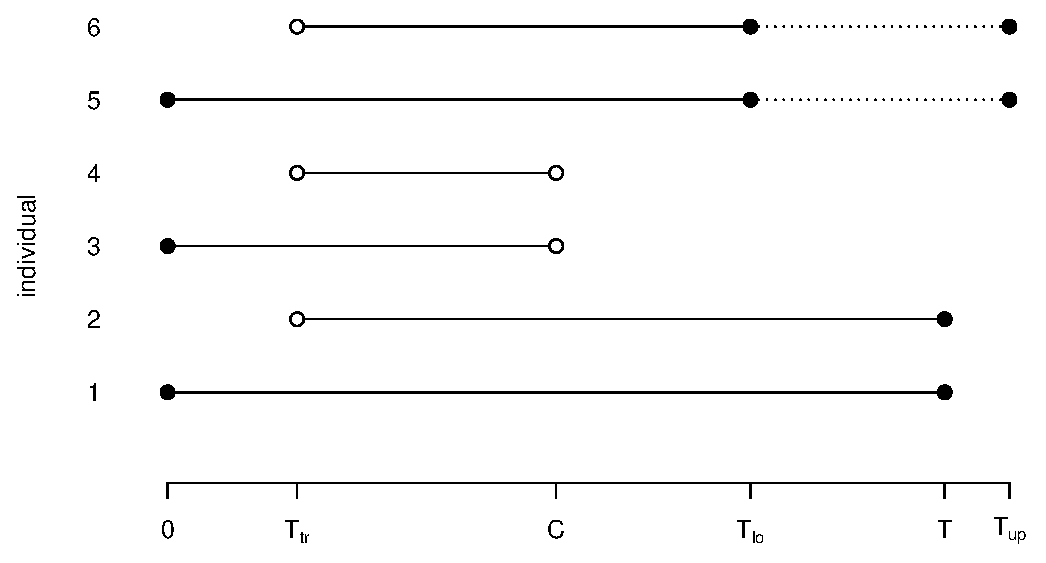
\epsfig{file=grafiken/censoringschemes.eps,scale=0.7}
{\it\caption{Illustration of different censoring
schemes.\label{censoringschemes}}}
\end{center}
\end{figure}

In a general framework an observation can now be uniquely described
 by the quadruple $(T_{tr},T_{lo},T_{up},\delta)$, with
\begin{center}
\begin{tabular}{ll}
$T_{lo}=T_{up}=T$, $\delta=1$ & if the observation is uncensored,\\
$T_{lo}=T_{up}=C$, $\delta=0$ & if the observation is right censored,\\
$T_{lo}<T_{up}$, $\delta=0$ & if the observation is interval censored.\\
\end{tabular}
\end{center}
For left truncated observations we have $T_{tr}>0$ while $T_{tr}=0$
for observations which are not truncated.

Based on these definitions we can now construct the likelihood
contributions for the different censoring schemes in terms of the
hazard rate $\lambda(t)$ and the survivor function
$S(t)=\exp(\int_0^t\lambda(u)du)$. Under the common assumption of
noninformative censoring and conditional independence, the
likelihood is given by
\begin{equation}\label{likelihood}
 L=\prod_{i=1}^n L_i,
\end{equation}
where
\[L_i = \lambda(T_{up})S(T_{up})/S(T_{tr}) = \lambda(T_{up})\exp\left(-\int_{T_{tr}}^{T_{up}}\lambda(t)dt\right)\]
for an uncensored observation,
\[L_i = S(T_{up})/S(T_{tr}) = \exp\left(-\int_{T_{tr}}^{T_{up}}\lambda(t)dt\right)\]
for a right censored observation and
\[L_i = (S(T_{lo})-S(T_{up}))/S(T_{tr}) = \exp\left(-\int_{T_{tr}}^{T_{lo}}\lambda(t)dt\right)\left(1-\exp\left(-\int_{T_{lo}}^{T_{up}}\lambda(t)dt\right)\right)\]
for an interval censored observation. Note that for explicit
evaluation of the likelihood (\ref{likelihood}) some numerical
integration technique has to be employed, since none of the
integrals can in general be solved analytically.

The above notation also allows for the easy inclusion of piecewise
constant, time-varying covariates via some data augmentation. Noting
that
\[\int_{T_{tr}}^{T}\lambda(t)dt = \int_{T_{tr}}^{t_1}\lambda(t)dt + \int_{t_1}^{t_2}\lambda(t)dt + \ldots + \int_{t_{p-1}}^{t_p}\lambda(t)dt + \int_{t_p}^{T}\lambda(t)dt\]
for $T_{tr}<t_1<\ldots<t_q<T$, we can replace an observation
$(T_{tr},T_{lo},T_{up},\delta)$ by a set of new observations
$(T_{tr},t_1,t_1,0)$, $(t_1,t_2,t_2,0)$, \ldots
$(t_{p-1},t_p,t_p,0)$, $(t_{p},T_{lo},T_{up},\delta)$ without
changing the likelihood. Therefore, observations with time-varying
covariates can be split up into several observations, where the
values $t_1<\ldots<t_p$ are defined by the changepoints of the
covariate and the covariate is now time-constant on each of the
intervals. In theory, other paths for a covariate $x(t)$ than
piecewise constant ones are also possible, if $x(t)$ is known for
$T_{tr}\le t\le T_{lo}$. In this case the the likelihood
(\ref{likelihood}) can also be evaluated numerically but a general
path $x(t)$ may lead to complicated data structures.

Figure \ref{timevaryingcovs} illustrates the data augmentation step
for a left truncated, uncensored observation and a covariate $x(t)$
that takes the three different values $x_1,x_2$ and $x_3$ on the
three intervals $[T_{tr},t_1], [t_1,t_2]$ and $[t_2,T_{up}]$. Here,
the original observation $(T_{tr},T_{up},T_{up},1)$ has to be
replaced by $(T_{tr},t_1,t_1,0)$, $(t_1,t_2,t_2,0)$ and
$(t_2,T_{up},T_{up},1)$.
\begin{figure}[htb]
\begin{center}
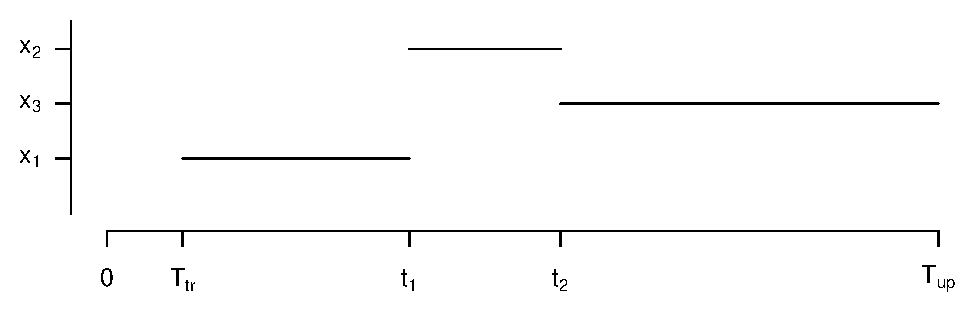
\epsfig{file=grafiken/timevaryingcovs.eps,scale=0.7}
{\it\caption{Illustration of time-varying
covariates.\label{timevaryingcovs}}}
\end{center}
\end{figure}

Currently, interval censored survival times can only be handled with
{\em remlreg objects}.

\subsection{Continuous-time multi-state models}\label{msmodels}
\index{Multi-state models}\index{Recurrent Events}\index{Disease
progression}\index{Competing risks}

Multi-state models are a flexible tool for the analysis of
time-continuous phenomena that can be characterized by a discrete
set of states. Such data structures naturally arise when observing a
discrete response variable for several individuals or objects over
time. Some common examples are depicted in Figure~\ref{some_msms} in
terms of their reachability graph for illustration. For recurrent
events (Figure~\ref{some_msms} (a)), the observations evolve through
time moving repeatedly between a fixed set of states. Other model
classes involve absorbing states, for example disease progression
models (Figure~\ref{some_msms} (b)), that are used to describe the
chronological development of a certain disease. If the severity of
this disease can be grouped into $q-1$ ordered stages of increasing
severity, a reasonable model might look like this: Starting from
disease state '$j$', an individual can only move to contiguous
states, i.e. either the disease gets worse and the individual moves
to state '$j+1$', or the disease attenuates and the individual moves
to state '$j-1$'. In addition, death is included as a further,
absorbing state '$q$', which can be reached from any of the disease
states. A model with several absorbing states is the competing risks
model (Figure~\ref{some_msms} (c)) where, for example, different
causes of death are analysed simultaneously.

\begin{figure}
\begin{center}
  \vspace{3mm}
 \mbox
 {
 \beginpicture
 \setcoordinatesystem units <0.65cm,0.65cm> point at 0 0
 \setlength{\unitlength}{0.65cm}

 \put {(a) Recurrent events} [Bl] at 0 16.5

 \put {\circle{1}} [Bl] at 7.5 12
 \put {\bf3} [Bl] at 7.35 11.85

 \put {\circle{1}} [Bl] at 5.5 14.5
 \put {\circle{1}} [Bl] at 9.5 14.5
 \put {\bf1} [Bl] at 5.35 14.35
 \put {\bf2} [Bl] at 9.35 14.35

 \arrow <3mm> [0.2,0.5] from 6.3 14.65 to 8.7 14.65
 \arrow <3mm> [0.2,0.5] from 8.7 14.35 to 6.3 14.35

 \arrow <3mm> [0.2,0.5] from  5.55 13.85 to 6.9 12.65
 \arrow <3mm> [0.2,0.5] from  7.25 12.65 to 5.9 13.85

 \arrow <3mm> [0.2,0.5] from  9.1 13.85 to 7.75 12.65
 \arrow <3mm> [0.2,0.5] from  8.1 12.65 to 9.45 13.85


 \put {(b) Disease progression} [Bl] at 0 10.5

 \put {\circle{1}} [Bl] at 7.5 6
 \put {$q$} [Bl] at 7.35 5.85

 \put {\circle{1}} [Bl] at 1.5 9
 \put {\circle{1}} [Bl] at 4.5 9
 \put {\circle{1}} [Bl] at 7.5 9
 \put {\circle{1}} [Bl] at 13.5 9
 \put {\bf1} [Bl] at 1.35 8.85
 \put {\bf2} [Bl] at 4.35 8.85
 \put {\bf3} [Bl] at 7.35 8.85
 \put {$q$-1} [Bl] at 13.15 8.85

 \put{$\cdots$} [Bl] at 10.1 8.9

 \arrow <3mm> [0.2,0.5] from 2.2 9.15 to 3.8 9.15
 \arrow <3mm> [0.2,0.5] from  3.8 8.85 to 2.2 8.85

 \arrow <3mm> [0.2,0.5] from 5.2 9.15 to 6.8 9.15
 \arrow <3mm> [0.2,0.5] from  6.8 8.85 to 5.2 8.85

 \arrow <3mm> [0.2,0.5] from 8.2 9.15 to 9.8 9.15
 \arrow <3mm> [0.2,0.5] from  9.8 8.85 to 8.2 8.85

 \arrow <3mm> [0.2,0.5] from 11.2 9.15 to 12.8 9.15
 \arrow <3mm> [0.2,0.5] from  12.8 8.85 to 11.2 8.85

 \arrow <3mm> [0.2,0.5] from  7.5 8.35 to 7.5 6.65
 \arrow <3mm> [0.2,0.5] from  4.75 8.35 to 7.0 6.65
 \arrow <3mm> [0.2,0.5] from  1.75 8.35 to 6.5 6.5
 \arrow <3mm> [0.2,0.5] from  13.25 8.35 to 8.5 6.5

 \put {(c) Competing risks} [Bl] at 0 4.5

 \put {\circle{1}} [Bl] at 1.5 0
 \put {\circle{1}} [Bl] at 4.5 0
 \put {\circle{1}} [Bl] at 7.5 0
 \put {\circle{1}} [Bl] at 13.5 0
 \put {\bf2} [Bl] at 1.35 -0.15
 \put {\bf3} [Bl] at 4.35 -0.15
 \put {\bf4} [Bl] at 7.35 -0.15
 \put {$q$} [Bl] at 13.35 -0.15

 \put {\circle{1}} [Bl] at 7.5 3
 \put {\bf1} [Bl] at 7.35 2.85

 \put{$\cdots$} [Bl] at 10.1 -0.1

 \arrow <3mm> [0.2,0.5] from  7.5 2.35 to 7.5 0.65

 \arrow <3mm> [0.2,0.5] from  6.9 2.6 to 4.75 0.65
 \arrow <3mm> [0.2,0.5] from  6.5 2.75 to 1.95 0.65
 \arrow <3mm> [0.2,0.5] from  8.5 2.75 to 12.85 0.65

 \endpicture
 }
 \vspace{3mm}

 \caption{Reachability graphs of some common multi-state
 models.\label{some_msms}}
\end{center}
\end{figure}

A multi-state model is fully described by a set of hazard rates
$\lambda_{hi}(t)$ where $h$, $h=1,\ldots,k$, indexes the type of the
transition and $i$, $i=1,\ldots,n$, indexes the individuals. Since
the hazard rates describe durations between transitions, we specify
them in analogy to hazard rate models for continuous time survival
analysis. To be more specific, $\lambda_{hi}(t)$ is modelled in a
multiplicative Cox-type way as
\[
 \lambda_{hi}(t) = \exp(\eta_{hi}(t)),
\]
where
\begin{equation}\label{addpred}
 \eta_{hi}(t) = g_{h0}(t) + \sum_{l=1}^Lg_{hl}(t)u_{il}(t) +
 \sum_{j=1}^Jf_{hj}(x_{ij}(t)) + v_i(t)'\gamma_h +  b_{hi}
\end{equation}
is an additive predictor consisting of the following components:
\begin{itemize}
 \item A time-varying, nonparametric baseline effect $g_{h0}(t)$ common for all
 observations.
 \item Covariates $u_{il}(t)$ with time-varying effects $g_{hl}(t)$.
 \item Nonparametric effects $f_{hj}(x_{ij}(t))$ of continuous covariates
 $x_{ij}(t)$.
 \item Parametric effects $\gamma_h$ of covariates $v_i(t)$.
 \item Frailty terms $b_{hi}$ to account for unobserved
 heterogeneity.
\end{itemize}

For each individual $i$, $i=1,\ldots,n,$ the likelihood contribution
in a multi-state model can be derived from a counting process
representation of the multi-state model. Let $N_{hi}(t)$,
$h=1,\ldots,k$ be a set of counting processes counting transitions
of type $h$ for individual $i$. Consequently, $h=1,\ldots,k$ indexes
the observable transitions in the model under consideration and the
jumps of the counting processes $N_{hi}(t)$ are defined by the
transition times of the corresponding multi-state process for
individual $i$.

From classical counting process theory (see e.g. \citeasnoun{Andetal93}, Ch.~VII.2), the intensity processes $\alpha_{hi}(t)$
of the counting processes $N_{hi}(t)$ are defined as the product of the hazard rate for type $h$ transitions $ \lambda_{hi}(t)$
and a predictable at-risk indicator process $Y_{hi}(t)$, i.e.
\[
 \alpha_{hi}(t) = Y_{hi}(t) \lambda_{hi}(t),
\]
where the hazard rates are constructed in terms of covariates as in
(\ref{addpred}). The at-risk indicator $Y_{hi}(t)$ takes the value
one if individual $i$ is at risk for a type $h$ transition at time
$t$ and zero otherwise. For example, in the multi-state model of
Figure~\ref{some_msms}a), an individual in state 2 is at risk for
both transitions to state 1 and state 3. Hence, the at-risk
indicators for both the transitions '2 to 1' and '2 to 3' will be
equal to one as long as the individual remains in state 2.

Under mild regularity conditions, the individual log-likelihood
contributions can now be obtained from counting process theory as
\begin{equation}\label{loglike1}
 l_i = \sum_{h=1}^k\left[ \int_0^{T_i}\log(\lambda_{hi}(t))dN_{hi}(t) -
 \int_0^{T_i}\lambda_{hi}(t)Y_{hi}(t)dt\right],
\end{equation}
where $T_i$ denotes the time until which individual $i$ has been
observed. The likelihood contributions can be interpreted similarly
as with hazard rate models for survival times (and in fact coincide
with these in the case of a multi-state process with only one
transition to an absorbing state). The first term corresponds to
contributions at the transition times since the integral with
respect to the counting process in fact equals a simple sum over the
transition times. Each of the summands is then given by the
log-intensity for the observed transition evaluated at this
particular time point. In survival models this term simply equals
the log-hazard evaluated at the survival time for uncensored
observations. The second term reflects cumulative intensities
integrated over accordant waiting periods between two successive
transitions. The integral is evaluated for all transitions the
corresponding person is at risk at during the current period. In
survival models there is only one such transition (the transition
from 'alive' to 'dead') and the integral is evaluated from the time
of entrance to the study to the survival or censoring time.

More details on multi-state models, including an exemplary analysis on human sleep, can be found in \citeasnoun{KneHen06}.

\addcontentsline{toc}{section}{Bibliography}

\begin{thebibliography}{99}

\harvarditem{Albert \& Chib}{1993}{AlbChi93}
 {\scshape Albert, J. \& Chib, S.} (1993).
 Bayesian analysis of binary and polychotomous response data.
 {\it Journal of the American Statistical Association}, {\bf 88}, 669--679.

\harvarditem{Andersen et al.}{1993}{Andetal93}
 {\scshape Andersen, P. K., Borgan, {\O}, Gill, R. D. \& Keiding, N.} (1993).
 {\it Statistical Models Based on Counting Processes.}
 New York: Springer Verlag.

\harvarditem{Andrews \& Mallows}{1974}{AndMal74}
 {\scshape Andrews, D. F. \& Mallows, C. L.} (1974).
 Scale mixtures of normal distributions.
 {\it Journal of the Royal Statistical Society B}, {\bf 36}, 99--102.

\harvarditem{Bollaerts, Eilers \& van Mechelen}{2006}{BolEilvMe06}
 {\scshape Albert, J. \& Chib, S.} (1993).
 Simple and Multiple P-Spline Regression with Shape Constraints.
 {\it British Journal of Mathematical and Statistical Psychology}, {\bf 59}, 451--469.

\harvarditem{Belitz}{2007}{Bel07}
 {\scshape Belitz, C.} (2007).
 {\it Model Selection in Generalized Structured Additive Regression Models.}
 PhD Thesis, University of Munich.

\harvarditem{Belitz \& Lang}{2008}{BelLan08}
{\scshape Belitz, C. \& Lang, S.} (2008).
 Simultaneous selection of variables and smoothing parameters in structured additive regression models.
{\it Computational Statistics and Data Analysis}, {\bf 53} , 61-81.

\harvarditem{Besag, York \& Molli\'{e}}{1991}{BesYorMol91}
 {\scshape Besag, J., York, J. \& Molli\'{e}, A.} (1991).
 Bayesian image restoration with two applications in spatial statistics (with discussion).
 {\it Annals of the Institute of Statistical Mathematics}, {\bf 43}, 1--59.

\harvarditem{Brezger \& Lang}{2006}{BreLan06}
 {\scshape Brezger, A. \& Lang, S.} (2006).
 Generalized additive regression based on Bayesian P-splines.
 {\it Computational Statistics and Data Analysis} {\bf 50}, 967--991.

\harvarditem{Devroye}{1986}{Dev86}
 {\scshape Devroye, L.} (1986).
 {\it Non-Uniform Random Variate Generation.}
 New York: Springer Verlag.

\harvarditem{Eilers \& Marx}{1996}{EilMar96}
 {\scshape Eilers, P. H. C. \& Marx, B. D.} (1996).
 Flexible smoothing using B-splines and penalized likelihood (with comments and rejoinder).
 {\it Statistical Science}, {\bf 11}, 89--121.

\harvarditem{Fahrmeir, Kneib \& Lang}{2004}{FahKneLan04}
 {\scshape Fahrmeir, L., Kneib, T. \& Lang, S.} (2004).
 Penalized structured additive regression for space-time data: A Bayesian perspective.
 {\it Statistica Sinica}, {\bf 14}, 715--745.

\harvarditem{Fahrmeir \& Lang}{2001}{FahLan01a}
 {\scshape Fahrmeir, L. \& Lang, S.} (2001a).
 Bayesian Inference for Generalized Additive Mixed Models Based on Markov Random Field Priors.
 {\it Journal of the Royal Statistical Society C}, {\bf 50}, 201--220.

\harvarditem{Fahrmeir \& Lang}{2001}{FahLan01b}
 {\scshape Fahrmeir, L. \& Lang, S.} (2001b).
 Bayesian Semiparametric Regression Analysis of Multicategorical Time-Space Data.
 {\it Annals of the Institute of Statistical Mathematics}, {\bf 53}, 10--30.

\harvarditem{Fahrmeir \& Osuna}{2006}{FahOsu06}
 {\scshape Fahrmeir, L. \& Osuna, L.} (2006).
 Structured additive regression for overdispersed and zero-inflated count data.
 {\it Applied Stochastic Models in Business and Industry}, {\bf 22}, 351--369

 \harvarditem{Fahrmeir \& Tutz}{2001}{FahTut01}
 {\scshape Fahrmeir, L. \& Tutz, G.} (2001).
 {\it Multivariate Statistical Modelling based on Generalized Linear Models.}
 New York: Springer-Verlag.

\harvarditem{Fotheringham, Brunsdon \& Charlton}{2002}{FotBruCha02}
 {\scshape Fotheringham, A. S., Brunsdon, C., \& Charlton, M. E.} (2002).
 {\it Geographically Weighted Regression: The Analysis of Spatially Varying Relationships.}
 Chichester: Wiley.

\harvarditem{Gamerman}{1997}{Gam97}
 {\scshape Gamerman, D.} (1997).
 Efficient Sampling from the posterior distribution in generalized linear models.
 {\it Statistics and Computing}, {\bf 7}, 57--68.

\harvarditem{Gelfand, Sahu \& Carlin}{1996}{GelSahCar96}
 {\scshape Gelfand, A. E., Sahu, S. K. \& Carlin, B. P.} (1996).
 Efficient Parametrizations for Genera\-lized Linear Mixed Models.
 In: Bernardo, J. M., Berger, J. O., Dawid, A. P. \& Smith, A. F. M. (eds.),
 {\it Bayesian Statistics 5}, 165--180.
 Oxford University Press.

\harvarditem{George \& Liu}{1981}{GeoLiu81}
 {\scshape George, A. \& Liu, J.W.} (1981).
 {\it Computer Solution of Large Sparse Positive Definite Systems.}
 Series in computational mathematics, Prentice-Hall.

\harvarditem{Green}{1987}{Gre87}
 {\scshape Green, P. J.} (1987).
 Penalized likelihood for general semiparametric regression models.
 {\it International Statistical Review}, {\bf 55}, 245--259.

\harvarditem{Green}{2001}{Gre01}
 {\scshape Green, P. J.} (2001).
 A Primer in Markov Chain Monte Carlo.
 In: Barndorff-Nielsen, O. E., Cox, D. R. \& Kl\"{u}ppelberg, C. (eds.),
 {\it Complex Stochastic Systems}, 1--62.
 Chapmann and Hall, London.

\harvarditem{Green \& Silverman}{1994}{GreSil94}
 {\scshape Green, P. J. \& Silverman, B.} (1994).
 {\it Nonparametric Regression and Generalized Linear Models.}
 Chapman and Hall, London.

\harvarditem{Griffin \& Brown}{2005}{GriBro05}
 {\scshape Griffin, J. E., and Brown, P. J.} (2005). Alternative prior distributions
 for variable selection with very many more variables than observations. Technical
 report, University of Warwick, Dept. of Statistics.

\harvarditem{Harville}{1977}{Har77}
 {\scshape Harville, D. A.} (1977).
 Maximum Likelihood approaches to variance component estimation and to related problems.
 {\it Journal of the American Statistical Association}, {\bf 72}, 320--338.

\harvarditem{Hastie \& Tibshirani}{1990}{HasTib90}
 {\scshape Hastie, T. \& Tibshirani, R.} (1990).
 {\it Generalized additive models.}
 Chapman and Hall, London.

\harvarditem{Hastie \& Tibshirani}{1993}{HasTib93}
 {\scshape Hastie, T. \& Tibshirani, R.} (1993).
 Varying-coefficient Models.
 {\it Journal of the Royal Statistical Society B}, {\bf 55}, 757--796.

\harvarditem{Hastie \& Tibshirani}{2000}{HasTib00}
 {\scshape Hastie, T. \& Tibshirani, R.} (2000).
 Bayesian Backfitting.
 {\it Statistical Science}, {\bf 15}, 193--223.

\harvarditem{Hastie, Tibshirani \& Firedman}{2001}{HasTibFri01}
 {\scshape Hastie, T., Tisbshirani, R. \& Friedman, J.} (2001).
 {\it The Elements of Statistical Learning: Data Mining, Inference and Prediction.}
 New York: Springer-Verlag.

\harvarditem{Hennerfeind, Brezger \& Fahrmeir}{2006}{HenBreFah06}
 {\scshape Hennerfeind, A., Brezger, A. \& Fahrmeir, L.} (2006).
 Geoadditive survival models.
 {\it Journal of the American Statistical Association}, {\bf 101}, 1065--1075.

\harvarditem{Holmes \& Held}{2006}{HolHel06}
 {\scshape Holmes, C., Held, L.} (2006).
 Bayesian auxiliary variable models for binary and multinomial regression.
 {\it Bayesian Analysis}, {\bf 1}, 145--168.

\harvarditem{Hurvich, Simonoff \& Tsai}{1998}{HurSimTsa98}
 {\scshape Hurvich, C. M., Simonoff, J. S. \& Tsai, C. L.} (1998).
 Smoothing parameter selection in nonparametric regression using an improved {A}kaike information criterion.
 {\it Journal of the Royal Statistical Society B}, {\bf 60}, 271--293.

\harvarditem{Ishwaran \& Rao}{2005}{IshRao05}
 {\scshape Ishwaran, H., and Rao, S. J.} (2005). Spike and Slab Variable
 Selection: Frequentist and Bayesian Strategies. {\it The Annals of Statistics},
 {\bf 33}, 730-773.

\harvarditem{Johnson, Moore \& Ylvisaker}{1990}{JohMooYlv90}
 {\scshape Johnson, M.E., Moore, L.M. \& Ylvisaker, D.} (1990).
 Minimax and maximin designs.
 {\it Journal of Statistical Planning and Inference}, {\bf 26}, 131--148.

\harvarditem{Kammann \& Wand}{2003}{KamWan03}
 {\scshape Kammann, E. E. \& Wand, M. P.} (2003).
 Geoadditive Models.
 {\it Journal of the Royal Statistical Society C}, {\bf 52}, 1--18.

\harvarditem{Kneib}{2006}{Kne06}
 {\scshape Kneib, T.} (2006).
 Geoadditive hazard regression for interval censored survival times.
 {\it Computational Statistics and Data Analysis}, {\bf 51}, 777--792

\harvarditem{Kneib \& Hennerfeind}{2006}{KneHen06}
 {\scshape Kneib, T. \& Hennerfeind, A.} (2006).
 Bayesian Semiparametric Multi-State Models.
 {\it Statistical Modelling}, {\bf 8}, 169--198.

\harvarditem{Kneib \& Fahrmeir}{2006}{KneFah06}
 {\scshape Kneib, T. \& Fahrmeir, L.} (2006).
 Structured additive regression for categorical space-time data: A mixed model approach.
 {\it Biometrics}, {\bf 62}, 109--118.

\harvarditem{Kneib \& Fahrmeir}{2007}{KneFah07}
 {\scshape Kneib, T. \& Fahrmeir, L.} (2007).
 A mixed model approach to structured hazard regression.
 {\it Scandinavian Journal of Statistics}, {\bf 34}, 207--228.

\harvarditem{Kneib et al.}{2009}{Kne09}
 {\scshape Kneib, T., Konrath, S. und Fahrmeir, L.} (2009). High-dimensional
 Structured Additive Regression Models: Bayesian Regularisation, Smoothing and Predictive
 Performance. Department of Statistics, Technical Report No. 46, LMU Munich.

\harvarditem{Knorr-Held}{1999}{KnoHel99}
 {\scshape Knorr-Held, L.} (1999).
 Conditional Prior Proposals in Dynamic Models.
 {\it Scandinavian Journal of Statistics}, {\bf 26}, 129--144.

\harvarditem{Konrath et al.}{2008}{Kon08}
 {\scshape Konrath, S., Kneib, T., Fahrmeir, L.} (2008). Bayesian Regularisation
 in Structured Additive Regression Models for Survival Data. Department of Statistics,
 Technical Report No.35, LMU Munich.

\harvarditem{Lang \& Brezger}{2004}{LanBre04}
 {\scshape Lang, S. \& Brezger, A.} (2004).
 Bayesian P-splines.
 {\it Journal of Computational and Graphical Statistics}, {\bf 13}, 183--212.

\harvarditem{Lin \& Zhang}{1999}{LinZha99}
 {\scshape Lin, X. \& Zhang, D.} (1999).
 Inference in generalized additive mixed models by using smoothing splines.
 {\it Journal of the Royal Statistical Society B}, {\bf 61}, 381--400.

\harvarditem{McCullagh \& Nelder}{1989}{McCNel89}
 {\scshape McCullagh, P. \& Nelder, J. A.} (1989).
 {\it Generalized Linear Models.}
 Chapman and Hall, London.

\harvarditem{M\"{u}ller, Stadtm\"{u}ller \& Tabnak}{1997}{MueStaTab97}
 {\scshape M\"{u}ller, H. G., Stadtm\"{u}ller, U. \& Tabnak, F.} (1997).
 Spatial Smoothing of Geographically Aggregated Data, with Applications to the Construction of Incidence Maps.
 {\it Journal of the American Statistical Association} {\bf 92}, 61--71.

\harvarditem{Nychka \& Saltzman}{1998}{NycSal98}
 {\scshape Nychka, D. \& Saltzman, N.} (1998).
 {\it Design of Air-Quality Monitoring Networks.}
 Lecture Notes in Statistics, 132, 51--76.

\harvarditem{Osuna}{2004}{Osu04}
 {\scshape Osuna, L.} (2004)
 {\it Semiparametric Bayesian Count Data Models}.
 Dr. Hut Verlag, M\"{u}nchen.

\harvarditem{Park \& Casella}{2008}{ParCas08}
 {\scshape Park, T., and Casella, G.} (2008). The Bayesian Lasso.
 {\it Journal of the American Statistical Association}, {\bf 482}, 681-686.

\harvarditem{Rue}{2001}{Rue01}
 {\scshape Rue, H.} (2001).
 Fast Sampling of Gaussian Markov Random Fields with Applications.
 {\it Journal of the Royal Statistical Society B}, {\bf 63}, 325--338.

\harvarditem{Ruppert, Wand \& Carroll}{2003}{RupWanCar03}
 {\scshape Ruppert, D., Wand, M. P. \& Carroll, R. J.} (2003).
 {\it Semiparametric Regression.}
 Cambridge University Press.

\harvarditem{Spiegelhalter et al.}{2002}{SpiBesCar02}
 {\scshape Spiegelhalter, D. J., Best, N. G., Carlin, B. P. \& van der Linde, A.} (2002).
 Bayesian measures of model complexity and fit.
 {\it Journal of the Royal Statistical Society B}, {\bf 65}, 583--639.

\end{thebibliography}

\addcontentsline{toc}{section}{Index}
\documentclass[11pt,a4paper,twoside]{bayesxarticle}

\input{manual_preliminaries.tex}

 \externaldocument{manual}
 \externaldocument{manual_tutorials}

 \makeindex

\begin{document}
\MakeShortVerb{\#}

\preface{Methodology Manual}

\newpage

\section{Introduction}

In this manual we provide a brief review of the methodological background for the three regression tools currently implemented
in {\em BayesX}. The first regression tool ({\em bayesreg objects}) relies on Markov chain Monte Carlo (MCMC) simulation
techniques and yields fully Bayesian posterior mean or posterior mode estimates. The second regression tool ({\em remlreg
objects}) is based on the mixed model representation of penalised regression models with inference being based on penalised
maximum likelihood and marginal likelihood (a generalisation of restricted maximum likelihood) estimation. The third regression
tool ({\em stepwisereg objects}) simultaneously performs model choice and estimation with inference being based on penalised
likelihood. MCMC techniques are partly used for computing interval estimates. All regression tools allow to estimate structured
additive regression (STAR) models (\citeasnoun{BelLan08}, \citeasnoun{BreLan06}, \citeasnoun{FahKneLan04}) with complex semiparametric predictors.
STAR models cover a number of well
known model classes as special cases, including {\em generalized additive models} \cite{HasTib90}, {\em generalized additive
mixed models} \cite{LinZha99}, {\em geoadditive models} \cite{KamWan03}, {\em varying coefficient models}\cite{HasTib93}, and
{\em geographically weighted regression} \citeasnoun{FotBruCha02}. Besides models for responses from univariate exponential
families, BayesX also supports non-standard regression situations such as models for categorical responses with either ordered
or unordered categories, continuous time survival data, or continuous time multi-state models. To provide a first impression of
structured additive regression, Sections~\ref{obsmodel} to \ref{inference} describe STAR models for exponential family
regression. Section~\ref{survivalAnalysis} extends structured additive regression to the analysis of survival times and
multi-state data. Full details on STAR methodology can be found in the following references:

\subsubsection*{Structured additive regression based on MCMC
simulation}

\begin{itemize}
\item Brezger, A., Lang, S. (2006): Generalized structured additive regression based on Bayesian P-Splines. {\it
    Computational Statistics and Data Analysis}, {\bf 50}, 967--991.
    \vspace{-0.25cm}
\item Brezger, A., Lang, S. (2008)
      Simultaneous Probability statements for Bayesian P-splines.
      {\it Statistical Modelling}, {\bf 8},
      141--168.\vspace{-0.25cm}
\item Brezger, A., Steiner, W. (2008)
Monotonic regression based on Bayesian P-splines: an
application to estimating price response functions from
store-level scanner data. {\it Journal of Economic and Business Statistics}, {\bf 26}, 90--104.
\vspace{-0.25cm}
\item Fahrmeir, L., Lang, S. (2001): Bayesian Inference for Generalized Additive Mixed Models Based on Markov Random Field
    Priors. {\it Journal of the Royal Statistical Society C (Applied Statistics)}, {\bf 50}, 201--220.\vspace{-0.25cm}
\item Fahrmeir, L., Lang, S. (2001): Bayesian Semiparametric Regression Analysis of Multicategorical Time-Space Data. {\it
    Annals of the Institute of Statistical Mathematics}, {\bf 53}, 10--30.\vspace{-0.25cm}
\item Fahrmeir, L., Osuna, L.. (2006): Structured additive regression for overdispersed and zero-inflated count data. {\it
    Applied Stochastic Models in Business and Industry}, {\bf 22}, 351--369.\vspace{-0.25cm}
\item Hennerfeind, A., Brezger, A., Fahrmeir, L. (2006): Geoadditive survival models. {\it Journal of the American
    Statistical Association}, {\bf 101}, 1065--1075.\vspace{-0.25cm}
\item Kneib, T., Hennerfeind, A. (2006) Bayesian Semiparametric Multi-State Models. {\it Statistical Modelling}, {\bf 8},
    169--198..\vspace{-0.25cm}
\item Lang, S., Brezger, A. (2004): Bayesian P-Splines {\it Journal of Computational and Graphical Statistics}, {\bf 13},
    183--212.
\end{itemize}

Presumably the best starting point is the paper by \citeasnoun{BreLan06}.

\begin{figure}[ht]
\footnotesize
\begin{center}
%\begin{tabular}{|p{8cm}|p{5cm}|}
%\hline
%{\bf Intended use} & {\bf recommended sections } \\
%\hline
%semiparametric regression, fully Bayesian approach  & sections \ref{obsmodel}, \ref{priorassumptions} , \ref{fullbayes} \\
%\hline
%semiparametric regression, inference based on mixed model technology, classical perspective &
%sections \ref{obsmodel}, \ref{penalizedleastsquares}, \ref{glmmrep}, \ref{glmmmeth} \\
%\hline
%semiparametric regression, inference based on mixed model technology, Bayesian point of view & sections \ref{obsmodel}, \ref{priorassumptions},
%\ref{glmmrep}, \ref{glmmmeth} \\
%\hline
%semiparametric regression including model choice & sections \ref{obsmodel}, \ref{penalizedleastsquares}, \ref{stepwiseest} \\
%\hline
%\end{tabular}
% \vspace{3mm}
\[\mbox{
 \beginpicture
 \setcoordinatesystem units <1.1cm,1.1cm> point at 0 0
 \setlength{\unitlength}{1.1cm}

 \put {\framebox(5.5,0.7){\sffamily\bfseries 2 Generalized regression models}} at 0 0

 \put {Bayesian perspective} at -4 -1.2
 \put {frequentist perspective} at 4 -1.2

 \arrow <4mm> [0.25,0.75] <0pt,5mm> from 0 -1 to -5 -2.9
 \arrow <4mm> [0.25,0.75] <0pt,5mm> from 0 -1 to 5 -2.9

 \put {\framebox(4.5,0.7){\sffamily\bfseries 4 Bayesian point of view}} at -5 -3

 \put {\framebox(4.5,0.7){\sffamily\bfseries 3 Penalised likelihood}} at 5 -3

 \arrow <4mm> [0.25,0.75] <0pt,5mm> from -5 -4 to 0 -6
 \arrow <4mm> [0.25,0.75] <0pt,5mm> from 5 -4 to 0 -6

 \put {relation to mixed models} at 0 -4.5

 \put {\framebox(5.5,0.7){\sffamily\bfseries 5 Mixed model representation}} at 0 -6

 \arrow <4mm> [0.25,0.75] <0pt,5mm> from -5 -4 to -5 -9
 \arrow <4mm> [0.25,0.75] <0pt,5mm> from 5 -4 to 5 -9

 \put {\framebox(3.5,0.7){\sffamily\bfseries 6.1 bayesreg objects}} at -5 -9
 \put {\framebox(3.5,0.7){\sffamily\bfseries 6.3 stepwisereg objects}} at 5 -9

 \put {MCMC (full Bayes)} at -6.5 -6
 \put {penalised likelihood} at 6.5 -5.75
 \put {incl. model choice} at 6.5 -6.15

 \arrow <4mm> [0.25,0.75] <0pt,5mm> from 0 -7 to 0 -9

 \put {penalised likelihood} at -1.5 -7.5
 \put {(empirical Bayes)} at 1.3 -7.5

 \put {\framebox(3.5,0.7){\sffamily\bfseries 6.2 remlreg objects}} at 0 -9


 \endpicture
}\]
 \vspace{3mm}

{\em \caption {\label{guideline} Guidelines for reading this
manual.}}
\end{center}
\end{figure}

\subsubsection*{Structured additive regression based on mixed model
methodology}

\begin{itemize}
\item Fahrmeir, L., Kneib, T., Lang, S. (2004): Penalized structured additive regression for space-time data: a Bayesian
    perspective. {\it Statistica Sinica}, {\bf 14}, 715--745.\vspace{-0.25cm}
\item Kneib, T. (2006): Mixed model based inference in structured additive regression. Dr. Hut Verlag, M\"{u}nchen. Available
    online from
    \href{http://edoc.ub.uni-muenchen.de/archive/00005011/}{http://edoc.ub.uni-muenchen.de/archive/00005011/}\vspace{-0.25cm}
\item Kneib, T. (2006): Geoadditive hazard regression for interval censored survival times. {\it Computational Statistics
    and Data Analysis}, {\bf 51}, 777--792.\vspace{-0.25cm}
\item Kneib, T., Fahrmeir, L. (2007): A mixed model approach for geoadditive hazard regression. {\it Scandinavian Journal
    of Statistics}, {\bf 34}, 207--228.\vspace{-0.25cm}
\item Kneib, T., Fahrmeir, L. (2006): Structured additive regression for multicategorical space-time data: A mixed model
    approach. {\it Biometrics}, {\bf 62}, 109--118.\vspace{-0.25cm}
\item Kneib, T., Hennerfeind, A. (2006): Bayesian Semiparametric Multi-State Models. {\it Statistical Modelling}, {\bf 8},
    169--198.
\end{itemize}

Presumably the best starting point is the paper by \citeasnoun{FahKneLan04} or the monograph by \citeasnoun{Kne06}.

\subsubsection*{Structured additive regression including model selection}

\begin{itemize}
\item Belitz, C. (2007): Model selection in Generalised Structured Additive Regression Models. Dr. Hut Verlag, M\"{u}nchen.
\item Belitz, C., Lang, S. (2008) Simultaneous selection of variables and smoothing parameters
in structured additive regression models. {\it
Computational Statistics and Data Analysis}, {\bf 53} , 61-81.
\end{itemize}

Presumably the best starting point is the paper by \citeasnoun{BelLan08}.

\subsubsection*{Guideline for the reader}


The rest of this manual is organized as follows:

The next section describes the general structure of STAR models for
distributions of the response variable belonging to an exponential
family. The following Sections \ref{penalizedleastsquares} -
\ref{inference} discuss alternative approaches for specifying and
estimating the different model terms in STAR models. Section
\ref{penalizedleastsquares} describes the models from a more
classical penalized least squares perspectives. A Bayesian point of
view is taken in Section \ref{priorassumptions}. The close
connection to mixed models is highlighted in Section \ref{glmmrep}.
Section \ref{inference} gives a brief outline of the various
inference techniques for STAR models. Fully Bayesian inference via
MCMC simulation techniques is the topic of Section \ref{fullbayes}.
Inference based on mixed model technology is sketched in Section
\ref{glmmmeth}. Simultaneous selection of relevant model terms and
estimation of the parameters is described in Section
\ref{stepwiseest}.

For most users of BayesX it is sufficient to read only parts of this
manual. Some recommendations are given in Figure \ref{guideline}.


\section{Generalized regression models}
\label{obsmodel}

\index{Generalized linear model}\index{Exponential family}
Generalized linear models assume that, given covariates $\uvec$ and
unknown parameters $\gammavec$, the distribution of the response
variable $y$ belongs to an exponential family, i.e.
\begin{equation}
\label{likel} p(y \, | \, \uvec) = \exp \left( \frac{y \theta -
b(\theta)}{\phi} \right) c(y,\phi)
\end{equation}
where $b(\cdot)$, $c(\cdot)$, $\theta$ and $\phi$ determine the specific response distribution. A list of the most common
distributions and their parameters can be found for example in \citeasnoun{FahTut01}, page 21. The mean
$\mu=E(y|\uvec,\gammavec)$ is linked to a linear predictor $\eta$ by
\begin{equation}
\label{glm} \mu=h(\eta) \qquad \eta= \uvec'\gammavec,
\end{equation}
where $h$ is a known response function and $\gammavec$ are unknown
regression parameters.

In most practical regression situations, however, we are facing at
least one of the following problems:
\begin{itemize}
\item For the {\em continuous covariates} in the data set, the assumption of a strictly linear
effect on the predictor may be not appropriate. \vspace{-0.2cm}
\item Observations may be {\em spatially correlated}.
\vspace{-0.2cm}
\item Observations may be {\em temporally correlated}.
\vspace{-0.2cm}
\item Complex interactions may be required to model the joint effect
of some of the covariates adequately. \vspace{-0.2cm}
\item  Heterogeneity among individuals or units may be not sufficiently described by covariates. Hence,
unobserved {\em unit or cluster specific heterogeneity} has to be
considered appropriately.
\end{itemize}
To overcome these difficulties, we replace the strictly linear
predictor in (\ref{glm}) by a structured additive predictor
\begin{equation}
\label{gampred} \eta=f_{1}(x_{1})+\ldots+f_j(x_j) +
\ldots+f_{p}(x_{p})+\uvec'\gammavec,
\end{equation}
where $x_j$ denote
covariates of different type and dimension, and $f_j$ are (not
necessarily smooth) functions of the covariates. The functions $f_j$
comprise usual nonlinear effects of continuous covariates, time
trends and seasonal effects, two-dimensional surfaces, varying
coefficient models, i.i.d. random intercepts and slopes as well as
spatial effects. STAR-models cover a number of special cases
well known from the literature, in particular {\em Generalized additive models (GAM)},
{\em Generalized additive mixed models (GAM)}, {\em Geoadditive models}, {\em Multilevel models},
{\em Varying coefficient models (VCM)}, {\em ANOVA type interaction models} and {\em geographically weighted regression}.

\section{Penalized least squares}
\label{penalizedleastsquares}

In BayesX, the nonlinear functions $f_j$ are modeled by a basis
functions approach, i.e. a particular nonlinear function $f$ is
approximated by a linear combination of basis functions:
$$
f(x) = \sum_{k=1}^{K} \beta_k B_k(x)
$$
The $B_k$ are known basis functions and $\betavec =
(\beta_1,\dots,\beta_K)'$ is a vector of unknown regression
coefficients to be estimated. Note that the term basis function in
our understanding is not limited to basis functions known from
nonparametric smoothing such as B-splines but also refers to
non-standard basis functions such as indicator functions for regions
or clusters. To ensure enough flexibility, typically a large number
of basis functions is defined. To avoid overfitting, a roughness
penalty on the regression coefficients is additionally specified. We
use quadratic penalties of the form $\betavec' \Pvec(\lambdavec)
\betavec$ where $\Pvec(\lambdavec)$ is a penalty matrix. The penalty
depends on one or multiple smoothing parameters $\lambdavec$ that
govern the amount of smoothness imposed on the function $f$. Most
penalty matrices are of the particular simple form
$\Pvec(\lambdavec) = \lambda \Kvec$ where $\lambda$ is a scalar
smoothing parameter. For {\em stepwisereg objects} more complicated
penalties are sometimes possible. They are an additive combination
of penalty matrices. An example is $\Pvec(\lambdavec) = \lambda_1
\Kvec_1+\lambda_2 \Kvec_2$ where $\lambda_1$ and $\lambda_2$ are
smoothing parameters and $\Kvec_1$ and $\Kvec_2$ are penalty
matrices.

The choice of basis functions $B_1,\dots,B_K$ and penalty  $\Pvec(\lambdavec)$ depends on our prior assumptions about the smoothness
of $f$ as well as
the type and dimension of $x$. We will give specific examples below. Defining the $n \times K$ design matrix $\Xvec$ with elements
$X[i,k] = B_k(x_i)$ the
vector $\fvec = (f(x_1),\dots,f(x_n))'$ of function evaluations can be written in matrix notation as $\fvec = \Xvec \betavec$.
Accordingly,  for model (\ref{gampred}) we obtain
$$
\etavec = \Xvec_1 \betavec_1 + \ldots + \Xvec_p \betavec_p + \Uvec \gammavec +  \varepsilonvec,
$$
where $\Uvec$ is the design matrix for linear effects, $\gammavec$ is the vector of regression coefficients for linear effects, and
$\varepsilonvec$
are the vectors of observations and errors.
In the next subsections we will give specific examples for modeling the unknown functions $f_j$ or in other words for the choice of basis functions and
penalty matrices.
We start with modeling the effect of continuous covariates using splines.

\subsection{Continuous covariates}
\subsubsection{P(enalized)-splines}
Suppose first that a particular component $x$ of the covariate  is univariate and continuous. There is a considerable amount of
literature on basis functions approaches in combination with a (quadratic) roughness penalty for continuous covariates. BayesX
applies the P-splines approach introduced by \citeasnoun{EilMar96}. The approach assumes that the unknown functions can be
approximated by a polynomial spline of degree $l$ and with equally spaced knots
$$
x_{min} = \zeta_{0}  < \zeta_{1} < \dots < \zeta_{m-1} < \zeta_{m} = x_{max}
$$
over the domain of $x$. The spline can be written in terms of a linear combination of $K=m+l$ B-spline basis functions. The
columns of the design matrix $\Xvec$ are given by the B-spline basis functions evaluated at the observations $x_i$. To overcome
the well known difficulties involved with regression splines, \citeasnoun{EilMar96} suggest a relatively large number of knots
(usually between 20 to 40) to ensure enough flexibility, and to introduce a roughness penalty on adjacent regression
coefficients based on squared $r$-th order differences, i.e.
$$
\betavec' \lambda \Kvec \betavec = \lambda \sum_{k=r+1}^K (\Delta^r \beta_k)^2.
$$
The penalty matrix is given by $\Kvec =  \Dvec_r' \Dvec_r$ where $\Dvec_r$ is a $r$-th order difference matrix.
Typically, second or third order differences are used. The limiting behavior $\lambda \rightarrow \infty$ depends both on the
order of the spline
and the order of the penalty. If the order of the spline is equal to or
higher than the order of  the penalty, which is typically the case, then a polynomial
fit of degree $r-1$ is obtained in the limit.

The approach can be extended to impose monotonicity or more general shape constraints. We follow an approach proposed by
\citeasnoun{BolEilvMe06}. A sufficient condition for a decreasing spline is given by $\beta_{k} \leq \beta_{k-1}$, i.e.  a
parameter $\beta_{k}$ is less than its predecessor $\beta_{k-1}$. The simple but powerful idea  is to impose the required
constraint by expanding the penalty by an additional  term. More specifically they propose the composed penalty
$$
\Pvec(\lambdavec) =  \betavec' \left( \lambda_1 \Kvec_1 + \lambda_2 \Kvec_2 \right) \betavec
$$
where $\lambda_1$ and $\Kvec_1$ are the usual smoothing parameter
and penalty matrix for P-splines. The additional penalty matrix
$\Kvec_2$ is a diagonal matrix with entries 1 whenever the condition
$\beta_{k} \leq \beta_{k-1}$ fails and 0 otherwise. For increasing
functions, $\Kvec_2$ has to be adapted accordingly. The parameter
$\lambda_2$ is not estimated but set large enough to enforce
monotonic functions.





\subsubsection{Tensor product P-splines}
\label{tensorproductpsplines} Assume now that $\xvec$ is
two-dimensional, i.e. $\xvec = \left(x^{(1)},x^{(2)}\right)'$ with
continuous components $x^{(1)}$ and $x^{(2)}$. The aim is to extend
the univariate P-spline from the preceding section to two
dimensions. A common approach is to approximate the unknown surface
$f(x)$ by the tensor product of one dimensional B-splines, i.e.
\begin{equation}
\label{gampspline_2dimterm} f\left(x^{(1)},x^{(2)}\right) = \sum_{k=1}^{K_1}
\sum_{s=1}^{K_2} \beta_{ks} B_{1,k}(x^{(1)})
B_{2,s} (x^{(2)}),
\end{equation}
where $B_{11},\dots,B_{1K_1}$ are the basis functions in $x^{(1)}$ direction and
$B_{21},\dots,B_{2K_2}$ in $x^{(2)}$ direction.
The $n \times K = n \times K_1 K_2$ design matrix $\Xvec$ now consists of
products of basis functions.

Several alternatives are available for the penalty matrix $\Pvec(\lambdavec)$:
\begin{enumerate}
\item[a)] {\em Penalty based on first differences:} The
two-dimensional generalization of a penalty based on first
differences is given by combining row- and column wise quadratic
differences
$$
\begin{array}{l}
\displaystyle \sum_{k=2}^{K_1}\sum_{s=1}^{K_2}(\beta_{ks}-\beta_{k-1,s})^2 =
\betavec'(\Ivec_{K_2}\otimes \Dvec_1)'(\Ivec_{K_2}\otimes \Dvec_1)\betavec \\[0.4cm]
\displaystyle  \sum_{k=1}^{K_1}\sum_{s=2}^{K_2}(\beta_{ks}-\beta_{k,s-1})^2 =
\betavec'(\Dvec_2\otimes \Ivec_{K_1})'(\Dvec_2\otimes \Ivec_{K_1})\betavec \\
\end{array}
$$
to the penalty
$$
\betavec'\Pvec(\lambdavec) \betavec =  \betavec' \lambda \left[ (\Ivec_{K_2}\otimes \Dvec_1)'(\Ivec_{K_2}\otimes \Dvec_1) + (\Dvec_2\otimes \Ivec_{K_1})'
(\Dvec_2\otimes \Ivec_{K_1})\right]\betavec.
$$
Another way of expressing the penalty is given by
\begin{equation}
\label{2dpenalty}
 \betavec'\Pvec(\lambda)\betavec = \betavec'\lambda \left[\Ivec_{K_2}\otimes\Kvec_1 + \Kvec_2\otimes \Ivec_{K_1}\right]\betavec,
\end{equation}
where $\Kvec_1$ and $\Kvec_2$ are the respective one dimensional penalty matrices.
In the limit  $\lambda \rightarrow \infty$ a constant fit is obtained.
\item[b)] {\em Penalty based on second differences:} In a similar way two-dimensional penalties based on higher order differences
are constructed. A second order difference penalty is obtained if
$\Kvec_1$ and $\Kvec_2$ in (\ref{2dpenalty}) correspond to penalty
matrices based on second rather than first differences. Similar to
one dimensional P-splines the limit $\lambda \rightarrow \infty$
results in linear effects in $x^{(1)}$ and $x^{(2)}$ with an
additional interaction effect, i.e.
$$
f\left(z^{(1)},z^{(2)}\right) = c_0 + c_1 \, x^{(1)} + c_2 \,
x^{(2)} + c_3 \, x^{(1)} x^{(2)}.
$$
\item[c)] {\em Anisotropic penalty:} The two penalties considered so far are not capable of
different penalization in $x^{(1)}$ and $x^{(2)}$ direction,
respectively. Anisotropic penalties are obtained by assuming
separate smoothing parameters $\lambda_1$ and $\lambda_2$ in
$x^{(1)}$ and $x^{(2)}$ direction. The penalty is then given by
\begin{equation}
\label{penalty_eilmar}
 \betavec'\Pvec(\lambdavec) \betavec = \betavec'\left[\lambda_1 \Ivec_{K_2}\otimes\Kvec_1 + \lambda_2 \Kvec_2\otimes \Ivec_{K_1}\right]\betavec.
\end{equation}
The resulting fit in the limit $\lambda_1 \rightarrow \infty$ and
$\lambda_2 \rightarrow \infty$ depends on the penalty used to
construct $\Kvec_1$ and $\Kvec_2$. If $\Kvec_1$ and $\Kvec_2$
correspond to a first order difference penalty a constant fit is
obtained in the limit. Second order difference penalties result in a
linear fit for $f\left(x^{(1)},x^{(2)}\right)$.
\item[d)] {\em Penalties with main effects in the limit:} Sometimes it is desirable to decompose the effect of the two covariates
$x^{(1)}$ and $x^{(2)}$ into two main effects modeled by one
dimensional functions and a two-dimensional interaction effect, i.e.
\begin{equation}
\label{pspline_2dimtermmain} f \left(x^{(1)},x^{(2)}\right) =
f_1\left(x^{(1)} \right) + f_2 \left(x^{(2)}\right) + f_{1|2}\left(
x^{(1)},x^{(2)} \right).
\end{equation}
Usually a two-dimensional surface smoother  together with two
additional  one dimensional P-splines (or other smoothers) are
estimated. This approach is possible with {\em bayesreg objects} and
{\em remlreg objects}. {\em stepwisereg objects} take, however, a
different approach. We specify a two-dimensional surface based on
tensor product P-splines and compute the decomposition of the
resulting surface into main effects and the interaction effect {\em
after} estimation. Moreover, we specify a penalty that allows for a
main effects only model as a special case. This allows to
discriminate between a simple  main effects model and a more
complicated two way interactions model. A penalty that guarantees  a
main effects model in the limit is defined by the Kronecker product
of the two penalty matrices for one dimensional P-splines, i.e.
\begin{equation}
\label{penalty_kronecker}
\betavec'\Pvec(\lambda)\betavec = \betavec' \lambda \Kvec_1 \otimes \Kvec_2 \betavec.
\end{equation}
The drawback of this penalty is that the limit $\lambda \rightarrow \infty $ yields {\em unpenalized} main effects, i.e. wiggly functions.
We therefore use a modified penalty which is effectively a combination of the two  penalties  (\ref{penalty_eilmar}) and
(\ref{penalty_kronecker}). More specifically
we define
\begin{equation}
\label{penalty_comb}
\betavec'\Pvec(\lambdavec)\betavec = \betavec' \left[\frac{\lambda_1}{K_1}
\Ivec_{K_2}\otimes\Kvec_1 + \frac{\lambda_2}{K_2} \Kvec_2\otimes \Ivec_{K_1}+\lambda_3 \Kvec_1 \otimes \Kvec_2   \right] \betavec,
\end{equation}
where $\Kvec_1$ and $\Kvec_2$ are penalty matrices corresponding to one dimensional P-splines based on first or second order differences.
This penalty has the following nice properties:
\begin{itemize}
\item The limit $\lambda_3 \rightarrow \infty$ results in a mere main effects model. The main effects  are one dimensional P-splines with smoothing
parameters $\lambda_1$ and $\lambda_2$.
\item The limit $\lambda_3 \rightarrow 0$ yields the anisotropic penalty (\ref{penalty_eilmar}) as a special case.
\item The limit $\lambda_1 \rightarrow 0$ and $\lambda_2 \rightarrow 0$  yields the Kronecker product penalty
(\ref{penalty_kronecker}) as a special case.
\item The limit $\lambda_1 \rightarrow \infty$, $\lambda_2 \rightarrow \infty$ and $\lambda_3 \rightarrow \infty$ results in a main effects model with
linear or constant main effects depending on the difference order used to construct $\Kvec_1$ and $\Kvec_2$.
\end{itemize}
\end{enumerate}


\subsection{Spatial effects}

In this subsection we assume that $x$ represents the location a
particular observation pertains to. The location is typically given
in two ways. If exact locations are available $x=(x^{(1)},x^{(2)})'$
is two-dimensional and the components  $x^{(1)}$ and $x^{(2)}$
correspond to the coordinates of the location. In this case, the
spatial effect $f(x^{(1)},x^{(2)})$ could be modeled by
two-dimensional surface estimators as described in the preceding
section.

In many applications, however, exact locations are not available. Typically, a geographical map is available and $x \in \{1,\dots,K\}$ is an
index that denotes the region (e.g. district) an observation pertains to. A common approach is to assume $f(x) = \beta_x$,
i.e. separate parameters $\beta_1,\ldots,\beta_K$  for each region are estimated.
The $n \times K$ design matrix $\Xvec$ is an incidence matrix whose entry in
the $i$-th row and $k$-th column is equal to one if observation $i$ has been observed at
location $k$ and zero otherwise. To prevent overfitting a penalty based on squared differences is defined that
guarantees that parameters of neighboring regions are similar. Typically two regions are assumed to be neighbors if they share a common
boundary although other neighborhood definitions are possible. The penalty is defined as
$$
\betavec' \lambda \Kvec \betavec = \lambda\sum_{k=2}^{K}\sum_{s \in N(k), s < k}(\beta_k-\beta_s)^2,
$$
where $N(k)$ denotes all sites that are neighbors of site $k$.
The elements of the penalty matrix are given by
\begin{equation}
\label{K_mrf}
 \Kvec[s,r] = \lambda \left\{
 \begin{array}{ll}
-1 & k\neq s, k\sim s,\\
 0 & k\neq s, k \nsim s,\\
 |N(k)| & k=s.
\end{array}
\right.
\end{equation}

Depending on the prior belief on smoothness of the spatial effect
several alternatives to penalty (\ref{K_mrf}) are available. If a
very smooth effect is assumed, the two-dimensional smoothers
discussed in the preceding section could be used as an alternative.
Since exact locations are not available the centroids of the regions
could be used instead.

\subsection{Unit- or cluster specific heterogeneity}
Typically, unit- or cluster specific random effects are introduced
to account for unobserved heterogeneity. In its simplest form, a
random intercept $\beta_x$ with $\beta_x \sim N(0,\tau^2)$ is
introduced. Here, $x \in \{1,\dots,K\}$ is an index variable that
denotes the cluster a particular observation pertains to. This is
equivalent to a penalized least squares approach with function $f(x)
= \beta_x$, penalty matrix $\Ivec$ and smoothing parameter $\lambda
= \sigma^2/\tau^2$. The $n \times K$ design matrix $\Xvec$ is a 0/1
incidence matrix whose entry in the $i$-th row and $k$-th column is
equal to one if observation $i$ belongs to the $k$-th cluster and
zero otherwise. Random slopes could be treated in the same way, see
the next subsection.

A particular cluster variable is a spatial index that indicates the region an observation pertains to. Usually a spatially correlated effect
as described in the preceding subsection is specified.
However, in some situations a smooth spatial effect is not justified because of local, spatial heterogeneity. In this case,
the assumption of spatial dependence of neighboring parameters is not meaningful. Instead, the simple (ridge type) penalty
$$
\betavec' \lambda \Kvec \betavec = \lambda \betavec'  \betavec = \lambda \sum_{k=1}^{K} \beta_k^2
$$
with penalty matrix $\Kvec = \Ivec$ may be defined. This penalty does not assume any spatial dependence but prevents highly variable
estimates induced by small samples for some regions or sites.

Note that more than one random intercept with respect to different
cluster variables are possible. In many cases there exists a
hierarchical ordering of clusters. Models with such hierarchical
clusters are also called multilevel models.


\subsection{Varying coefficients}
\label{varcoeff_terms}

Suppose now that the effect of a continuous covariate $x^{(2)}$ is assumed to vary with
respect to a categorical covariate $x^{(1)}$. For notational convenience, we restrict the discussion to binary covariates $x^{(1)}$.
The generalization to (multi)categorical covariates is straightforward.
The interaction between $x^{(2)}$ and
$x^{(1)}$ can be modeled by a predictor of the form
$$
\eta = \ldots + f_1(x^{(2)}) + g(x^{(2)}) x^{(1)} + \ldots,
$$
where $f_1$ and $g$ are smooth functions (modeled by P-splines). The
interpretation of the two functions $f_1$ and $g$ depends on the
coding of the binary variable $x^{(1)}$. If $x^{(1)}$ is in
dummy-coding, the function $f_1$ corresponds to the effect of
$x^{(2)}$ subject to  $x^{(1)}=0$, and $g$ is the difference effect
for observations with $x^{(1)}=1$. If $x^{(1)}$ is in effect-coding,
the function $f_1$ can be interpreted as an average effect of
$x^{(2)}$, where $g$ and $-g$ represent the deviation from $f_1$ for
$x^{(1)} = 1$ and $x^{(1)} = -1$, respectively. It turns out that
the coding of $x^{(2)}$ is not only important  for interpretation
but sometimes also crucial for inference (in {\em bayesreg objects}
and {\em stepwisereg objects}). Estimation for {\em bayesreg and
stepwisereg objects} described in the next section is based on an
iterative backfitting type procedure. Hence dependence between $f_1$
and $g$ should be minimized to avoid convergence problems. Hence,
effect coding for $x^{(2)}$ is an effective yet simple device to
avoid convergence problems.

Models with interaction effects of the form $g(x^{(2)}) \, x^{(1)}$ are  known as varying coefficient models  because the
effect of $x^{(1)}$ varies smoothly with respect to the continuous covariate $x^{(2)}$. Covariate $x^{(2)}$ is called the
effect modifier of $x^{(1)}$. The approach can be easily extended to a two-dimensional effect modifier with components
$x^{(2)}$ and $x^{(3)}$. The interaction effect is then given by $g(x^{(2)},x^{(3)}) \, x^{(1)}$ where $g(x^{(2)},x^{(3)})$ is
a two-dimensional surface which is modeled by the tensor product P-splines discussed in section \ref{tensorproductpsplines}.
Another modification arises if the effect modifier is the location either given as the coordinates or as a spatial index. In
this case we have a space varying effect of $x^{(1)}$. Models of this kind are also known as geographically weighted
regression, see \citeasnoun{FotBruCha02}. A final modification is obtained for a unit or cluster index as effect modifier. The
effect of $x^{(1)}$ is now assumed to be unit- or cluster-specific and typically referred to as a random slope.

Independent of the specific type of the effect modifier, the interaction term $g\left(x^{(2)}\right) \, x^{(1)}$
(or $g\left(x^{(2)},x^{(3)}\right) \, x^{(1)}$) can be cast into our
general framework by defining
\begin{equation}
\label{gampspline_varcoeffterm}
f\left(x^{(1)},x^{(2)}\right) = g\left(x^{(2)}\right) \, x^{(1)} \quad \mbox{or} \quad  f\left(x^{(1)},x^{(2)},x^{(3)}\right) =
g\left(x^{(2)},x^{(3)}\right) \, x^{(1)}.
\end{equation}
The overall design matrix $\Xvec$ is given by
$\diag(x_{1}^{(1)},\dots,x_{n}^{(1)}) \, \Xvec^{(1)}$ where
$\Xvec^{(1)}$ is the usual design matrix for P-Splines, tensor
product P-splines, spatial-, or cluster-specific effects.



\section{Bayesian point of view}
\label{priorassumptions}\index{Prior assumptions}

For Bayesian inference, the unknown functions $f_{1},\dots ,f_{p}$
in predictor (\ref{gampred}), more exactly corresponding vectors of
function evaluations, and the fixed effects parameters $\gammavec$ are
considered as random variables and must be supplemented by
appropriate prior assumptions.

In the absence of any prior knowledge, diffuse priors are the
appropriate choice for fixed effects parameters, i.e.
$$
 p(\gamma_j) \propto const
$$
Another common choice, not yet supported by {\em BayesX}, are
informative multivariate Gaussian priors with mean $\muvec_0$ and
covariance matrix $\Sigmavec_0$.\index{Prior assumptions!Fixed effects}


Priors for the unknown functions $f_{1},\dots,f_{p}$ depend on the
{\em type of the covariates} and on {\em prior beliefs about the
smoothness of $f_j$.} In the following we express the vector of
function evaluations $\fvec_j=(f_j(x_{1j}),\dots,f_j(x_{nj}))'$ of a
function $f_j$ as the matrix product of a design matrix $\Xvec_j$ and a
vector of unknown parameters $\betavec_j$, i.e.
\begin{equation}
\label{matproduct} \fvec_j=\Xvec_j \betavec_j.
\end{equation}
Then, we obtain the predictor (\ref{gampred}) in matrix notation
as
\begin{equation}
\label{gampredmatrix} \etavec = \Xvec_1 \betavec_1 + \cdots + \Xvec_p \betavec_p +
\Uvec \gammavec,
\end{equation}
where $\Uvec$ corresponds to the usual design matrix for fixed
effects.

A prior for a function $f_j$ is defined by specifying a suitable
design matrix $\Xvec_j$ and a prior distribution for the vector
$\betavec_j$ of unknown parameters. The general form of the prior for
$\betavec_j$ is given by
\begin{equation}
\label{genform} p(\betavec_j | \tau_j^2) \propto
\frac{1}{(\tau^2_j)^{rank(\Kvec_j)/2}} \exp\left(-\frac{1}{2\tau_j^2}
\betavec_j' \Kvec_j \betavec_j\right),
\end{equation}
where $\Kvec_j$ is a {\em penalty matrix}. In most cases $\Kvec_j$ will be
rank deficient and therefore the prior for $\betavec_j$ is partially improper.

The variance parameter $\tau_j^2$ is  equivalent to the inverse
smoothing parameter in a penalized likelihood approach and controls the
trade off between flexibility and smoothness.

In the following we will describe specific priors for different
types of covariates and functions $f_j$.


\subsection{Continuous covariates}
\label{psplines}\index{Continuous covariates}\index{Time scales}
\index{Prior assumptions!Continuous covariates}

Several alternatives have been  proposed for specifying smoothness priors for continuous covariates or time scales. These are
{\em random walk priors} or more generally {\em autoregressive priors} (see \citeasnoun{FahLan01a} and \citeasnoun{FahLan01b},
{\em Bayesian P-splines} \cite{LanBre04} and {\em Bayesian smoothing splines} \cite{HasTib00}. {\em BayesX} supports random
walk priors and P-splines.

\subsubsection{Random walks}\index{Random walk priors}

Suppose first that $x$ is a time scale or continuous covariate
with equally spaced ordered observations
$$
x^{(1)} < x^{(2)} < \cdots < x^{(K)}.
$$
Here $K \leq n$ denotes the number of {\em different} observed
values for $x$ in the data set. A common approach in dynamic or
state space models is to estimate one parameter $\beta_{k}$ for
each distinct $x^{(k)}$, i.e. $f(x^{(k)}) = \beta_{k}$, and
penalize too abrupt jumps between successive parameters using random
walk priors. For example, first and second order random walk models
are given by
\begin{equation}
\label{rwpriors}
\beta_{k}=\beta_{k-1}+u_{k}\,\,\,\,\mbox{and}\,\,\,\,\beta_{k}=2\beta_{k-1}-\beta_{k-2}+u_{k}
\end{equation}
with Gaussian errors $u_{k}\sim N(0,\tau^{2})$ and diffuse priors
$p(\beta_{1})\propto const$, and $p(\beta_{1})$ and
$p(\beta_{2})\propto const$, for initial values, respectively. Both
specifications act as smoothness priors that penalize too rough
functions $f$. A first order random walk penalizes abrupt jumps
$\beta_{k}-\beta_{k-1}$ between successive states while a second
order random walk penalizes deviations from the linear trend $2
\beta_{k-1}-\beta_{k-2}$. The joint distribution of the
regression parameters $\betavec$ is easily computed as the product of
conditional densities defined by (\ref{rwpriors}) and can be brought
into the general form (\ref{genform}). The penalty matrix is of the
form $\Kvec=\Dvec'\Dvec$ where $\Dvec$ is a first or second order difference
matrix. For example, for a random walk of first order the penalty
matrix is given by:
$$
\Kvec = {\footnotesize \left(
\begin{array}{rrrrr}
 1 & -1 & & &  \\
-1 & 2 & -1 & & \\
 &  \ddots & \ddots & \ddots &  \\
 & & -1 & 2 & -1 \\
  & & & -1 & 1
\end{array}
\right) }.
$$
The design matrix $\Xvec$ is a simple 0/1 matrix where the number of
columns equals the number of parameters, i.e. the number of distinct
covariate values. If for the $i$-th observation $x_{i}=x^{(k)}$
the element in the $i$-th row and $k$-th column of $\Xvec$ is one and
zero otherwise.

In case of non-equally spaced observations slight modifications of the priors defined in (\ref{rwpriors}) are necessary, see
\citeasnoun{FahLan01a} for details.

\subsubsection{P-splines}\index{P-splines}

A second approach for effects of continuous covariates, that is closely related to random walk models, is based on P-splines
introduced by \citeasnoun{EilMar96}. The approach assumes that an unknown smooth function $f$ of a covariate $x$ can be
approximated by a polynomial spline of degree $l$ defined by a set of equally spaced knots $x_{min} = \zeta_{0}  < \zeta_{1} <
\dots < \zeta_{m-1} < \zeta_{m} = x_{max}$ within the domain of $x$. Such a spline can be written in terms of a linear
combination of $K = m+l$ B-spline basis functions $B_{k}$, i.e.
$$
f(x) = \sum_{k=1}^{K} \beta_{k} B_{k}(x).
$$
In this case, $\betavec = (\beta_{1},\dots,\beta_{K})'$ corresponds to the vector of unknown regression coefficients and the $n
\times K$ design matrix $\Xvec$ consists of the basis functions evaluated at the observations $x_{i}$, i.e. $\Xvec[i,k] =
B_k(x_{i})$. The crucial point is the choice of the number of knots. For a small number of knots, the resulting spline may not
be flexible enough to capture the variability of the data. For a large number of knots, estimated curves tend to overfit the
data and, as a result, too rough functions are obtained. As a remedy, \citeasnoun{EilMar96} suggest a moderately large number
of equally spaced knots (usually between 20 and 40) to ensure enough flexibility, and to define a roughness penalty based on
first or second order differences of adjacent B-Spline coefficients to guarantee sufficient smoothness of the fitted curves.
This leads to penalized likelihood estimation with penalty terms
\begin{equation}
\label{diffpenalty} \lambda \sum_{k=r+1}^{K}
(\Delta^r \beta_{k})^2 , \quad r=1,2
\end{equation}
where $\lambda$ is the smoothing parameter. First order differences penalize abrupt jumps $\beta_{k}-\beta_{k-1}$ between
successive parameters while second order differences penalize deviations from the linear trend $2 \beta_{k-1}-\beta_{k-2}$. In
a Bayesian approach we use the stochastic analogue of difference penalties, i.e. first or second order random walks, as priors
for the regression coefficients. Note that simple first or second order random walks can be regarded as P-splines of degree
$l=0$ and are therefore included as a special case. More details about Bayesian P-splines can be found in \citeasnoun{LanBre04}
and \citeasnoun{BreLan06}.

\subsubsection{Tensor product P-splines}
\label{tensorproductpsplines_bayes}

Assume now that $x$ is two-dimensional, i.e. $x = \left(x^{(1)},x^{(2)}\right)'$ with continuous components $x^{(1)}$ and
$x^{(2)}$. Similar to section \ref{tensorproductpsplines} the aim is to extend the univariate P-spline to two dimensions. In
{\em BayesX} Bayesian surface fitting is based on two-dimensional P-splines described in more detail in \citeasnoun{LanBre04}
and \citeasnoun{BreLan06}. The unknown surface $f(x^{(1)},x^{(2)})$ is approximated by the tensor product of two
one-dimensional B-splines, i.e.
$$
f\left(x^{(1)},x^{(2)}\right) = \sum_{k=1}^{K_1}
\sum_{s=1}^{K_2} \beta_{ks} B_{1,k}(x^{(1)})
B_{2,s} (x^{(2)}),
$$
where $B_{11},\dots,B_{1K_1}$ are the basis functions in $x^{(1)}$ direction and
$B_{21},\dots,B_{2K_2}$ in $x^{(2)}$ direction.
The $n \times K = n \times K_1 K_2$ design matrix $\Xvec$ now consists of
products of basis functions.

Priors for
$\betavec = (\beta_{11},\dots,\beta_{K_1,K_2})'$ can be based on
spatial smoothness priors common in spatial statistics, e.g.
two-dimensional first order random walks. The most commonly used
prior specification based on the four nearest neighbors is defined
by
\begin{equation}
\label{2dimrw1} \beta_{ks} | \cdot \sim N \left(
\frac{1}{4} ( \beta_{k-1,s}+ \beta_{k+1,s} +
\beta_{k,s-1} +\beta_{k,s+1}),\frac{\tau^2}{4}
\right)
\end{equation}
and appropriate edge corrections. This
prior as well as higher order bivariate random walks can be easily
brought into the general form (\ref{genform}).


\subsection{Spatial effects}\index{Spatial
priors}\index{Markov random fields}\index{Kriging}\index{Gaussian
random fields} \label{spatial}\index{Prior assumptions!Spatial
effects}

\subsubsection{Markov random fields}

Suppose that the index $s \in \{ 1,\dots,S \}$ represents the
location or site in connected geographical regions. For simplicity
we assume that the regions are labelled consecutively. A common way
to introduce a spatially correlated effect is to assume that
neighboring sites are more alike than arbitrary sites. Thus, for a
valid prior definition a set of neighbors for each site $s$ must be
defined. For geographical data one usually assumes that two sites
$s$ and $s'$ are neighbors if they share a common boundary.

The simplest (but most frequently used) spatial smoothness prior for
the function evaluations $f(s)=\beta_{s}$ is given by
\begin{equation}
\label{adjacency} \beta_{s} | \beta_{s'}, \, {s \neq
s'},\tau^2 \sim N \left( \frac{1}{N_s} \sum_{s' \in \partial_s}
\beta_{s'} , \frac{\tau^2}{N_s} \right),
\end{equation}
where $N_s$ is the number of adjacent sites and $s' \in
\partial_s$ denotes that site $s'$ is a neighbor of site $s$. Hence,
the (conditional) mean of $\beta_{s}$ is an unweighted average of
function evaluations of neighboring sites. The prior is a direct
generalization of a first order random walk to two-dimensions and is
called a Markov random field (MRF).

The $n \times S$ design matrix $\Xvec$ is a 0/1 incidence matrix. Its
value in the $i$-th row and the $s$-th column is 1 if the $i$-th
observation is located in site or region $s$, and zero otherwise.
The $S \times S$ penalty matrix $\Kvec$ has the form of an adjacency
matrix.

\subsubsection{Kriging}

If exact locations $\svec=(s_x,s_y)$ are available, we can use two-dimensional surface estimators to model spatial effects. One
option are two-dimensional P-splines, described in \autoref{tensorproductpsplines}. Another option are Gaussian random field
(GRF) priors, originating from geostatistics. These can also be interpreted as two-dimensional surface smoothers based on
radial basis functions and have been employed by \citeasnoun{KamWan03} to model the spatial component in Gaussian regression
models. The spatial component $f(\svec)=\beta_\svec$ is assumed to follow a zero mean stationary Gaussian random field
$\{\beta_\svec:\svec\in\mathbb{R}^2\}$ with variance $\tau^2$ and isotropic correlation function
$\Cov(\beta_\svec,\beta_{\svec+\hvec})=C(||\hvec||)$. This means that correlations between sites that are $||\hvec||$ units
apart are the same, regardless of direction and the sites location. For a finite array $\svec\in\{\svec_1,\ldots,\svec_S\}$ of
sites as in image analysis, the prior for $\betavec=(\beta_1,\ldots,\beta_S)'$ is of the general form (\ref{genform}) with
$\Kvec=\Cvec^{-1}$ and
\[\Cvec(i,j)=C(||\svec_i-\svec_j||), 1\le i,j\le S.\]
The design matrix $X$ is again a 0/1 incidence matrix.

Several proposals for the choice of the correlation function
$C(r)$ have been made. In the kriging literature, the Mat\'{e}rn
family $C(r;\rho,\nu)$ is highly recommended. For prechosen values $\nu=m+1/2$,
$m=0,1,2,\ldots$ of the smoothness parameter $\nu$ simple
correlation functions $C(r;\rho)$ are obtained, e.g.
\[C(r;\rho)=\exp(-|r/\rho|)(1+|r/\rho|)\]
with $\nu=1.5$. The parameter $\rho$ controls how fast correlations
die out with increasing $r=||h||$. It can be determined in a
preprocessing step or may be estimated jointly with the variance
components by restricted maximum likelihood. A simple rule, that
also ensures scale invariance of the estimates, is to choose $\rho$
as
\[\hat{\rho}=\max_{i,j}||\svec_i-\svec_j||/c.\]
The constant $c>0$ is chosen in such a way, that $C(c)$ is small,
e.g. 0.001. Therefore the different values of
$||\svec_i-\svec_j||/\hat{\rho}$ are spread out over the $r$-axis of
the correlation function. This choice of $\rho$ has proved to work
well in our experience.

\subsubsection{Discrete vs. continuous spatial smoothing}

Although we described them separately, approaches for exact locations can also be used in the case of connected geographical
regions, e.g. based on the centroids of the regions. Conversely, we can also apply MRFs to exact locations if neighborhoods are
defined based on a distance measure. In general, it is not clear which of the different approaches leads to the ''best'' fits.
For data observed on a discrete lattice MRFs seem to be most appropriate. If the exact locations are available, surface
estimators may be more natural, particularly because predictions for unobserved locations are available. However, in some
situations surface estimators lead to an improved fit compared to MRF's even for discrete lattices and vice versa. A general
approach that can handle both situations is given by \citeasnoun{MueStaTab97}.

From a computational point of view MRF's and P-splines are preferable to GRF's because their posterior precision matrices are
band matrices or can be transformed into a band matrix like structure. This special structure considerably speeds up
computations, at least for inference based on MCMC techniques. For inference based on mixed models, the main difference between
GRFs and MRFs, considering their numerical properties, is the dimension of the penalty matrix. For MRFs the dimension of $K$
equals the number of different regions $S$ and is therefore independent from the sample size. On the other side, for GRFs, the
dimension of $K$ is given by the number of distinct locations, which is usually close to the sample size. Therefore, the number
of regression coefficients used to describe a MRF is usually much smaller than for a GRF and therefore the estimation of GRFs
is computationally much more expensive. To overcome this difficulty \citeasnoun{KamWan03} propose low-rank kriging to
approximate stationary Gaussian random fields. Note first, that we can define GRFs equivalently based on a design matrix
$\Xvec$ with entries $\Xvec[i,j]=C(||\svec_i-\svec_j||)$ and penalty matrix $\Kvec=\Cvec$. To reduce the dimensionality of the
estimation problem we define a subset of knots $\mathcal{D}=\{\kappavec_1,\ldots,\kappavec_M\}$ of the set of distinct
locations $\mathcal{C}$. These knots can be chosen to be ''representative'' for the set of distinct locations $\mathcal{C}$
based on a space filling algorithm. Therefore consider the distance measure
\[d(\svec,\mathcal{D})=\left(\sum_{\kappavec\in\mathcal{D}}||\svec-\kappavec||^p\right)^{\frac{1}{p}},\]
with $p<0$, between any location $\svec\in\mathcal{D}$ and a
possible set of knots $\mathcal{C}$. Obviously this distance measure
is zero for all knots. Using a simple swapping algorithm to minimize
the overall coverage criterion
\[\left(\sum_{\svec\in\mathcal{C}}d(\svec,\mathcal{D})^q\right)^{\frac{1}{q}}\]
with $q>0$ (compare \citeasnoun{JohMooYlv90} and \citeasnoun{NycSal98} for details) yields an optimal set of knots
$\mathcal{D}$. Based on these knots we define the approximation $\fvec=\Xvec\betavec$ with the $n\times M$ design matrix
$\Xvec[i,j]=C(||\svec_i-\kappavec_j||)$, penalty matrix $\Kvec=\Cvec$, and $\Cvec[i,j]=C(||\kappavec_i-\kappavec_j||)$. The
number of knots $M$ allows to control the trade-off between accuracy of the approximation ($M$ close to the sample size) and
numerical simplification ($M$ small).

\subsection{Unit- or cluster-specific heterogeneity}
\label{random}\index{Random effects}\index{Group
indicators}\index{Unstructured spatial effects}

In many situations we observe the problem of heterogeneity among
clusters of observations caused by unobserved covariates. Neglecting
unobserved heterogeneity may lead to considerably biased estimates
for the remaining effects as well as false standard error estimates.
Suppose now $x \in \{1,\dots,K\}$ is a cluster variable indicating the
cluster a particular observation belongs to. A common approach to
overcome the difficulties of unobserved heterogeneity is to
introduce additional Gaussian i.i.d. effects $f(x) = \beta_{x}$
with
\begin{equation}
\label{randomeff} \beta_{x} \sim N(0,\tau^2), \quad
x=1,\dots,K.
\end{equation}
The design matrix $\Xvec$ is again a $n \times K$-dimensional 0/1
incidence matrix that represents the grouping structure of the data,
while the penalty matrix is simply the identity matrix, i.e.
$\Kvec=\Ivec$. From a classical perspective, (\ref{randomeff}) defines
i.i.d. {\em random effects}. However, from a Bayesian point of view
all unknown parameters are assumed to be random and hence the
notation "random effects" in this context is misleading. Hence, one
may also think of (\ref{randomeff}) as an approach for modelling an
unsmooth function.

Prior (\ref{randomeff}) may also be used for a more sophisticated
modelling of spatial effects. In some situation it may be useful to
split up the spatial effect $f_{spat}$ into a spatially correlated
(structured) part $f_{str}$ and a spatially uncorrelated
(unstructured) part $f_{unstr}$, i.e.
$$
f_{spat} = f_{str}+f_{unstr}.
$$
A rationale is that a spatial effect is usually a surrogate of many unobserved influential factors, some of which obeying a
strong spatial structure while others are present only locally. By estimating a structured and an unstructured component we aim
at distinguishing between the two kinds of influential factors, see also \citeasnoun{BesYorMol91}. For the smooth spatial part
we can assume any of the spatial priors discussed in \autoref{spatial}. For the uncorrelated part we may assume prior
(\ref{randomeff}).

\subsection{Varying coefficients}
\index{Varying coefficient models}

The models considered so far are not appropriate for modelling interactions between covariates. A common approach is based on
varying coefficient models introduced by \citeasnoun{HasTib93} in the context of smoothing splines. Varying coefficient terms
have already been discussed in the previous chapter, see section \ref{varcoeff_terms}.


\subsection{Regularization Priors for highdimensional covariates}
\label{Regularization Priors for highdimensional covariates}
\index{Regularization Priors for highdimensional covariates}

In this section the vector $\beta _{s} =\left(\beta _{p+1} ,\ldots\beta _{p+q} \right)$ is a subvector of unknown regression
coefficients $\gamma $ for fixed (linear) effects. A desirable feature for variable selection is to shrink small effects to
zero but to shrink important effects only moderately to prevent them from large bias. At the opposite to the unregularized
regression coefficients, where flat priors $p \left(\gamma \right)\propto 1$ are assumed we need here informative priors
appropriate for shrinkage. Several alternatives have been proposed for specifying shrinkage priors for the regression
coefficients, see e.g. Griffin and Brown (2005). Three shrinkage priors, which are hierarchically represented as scale mixtures
of normals, are implemented in {\em BayesX}, i.e. the {\em ridge}-, the {\em lasso}- and the {\em Normal Mixture of Inverse
Gamma (NMIG)-prior}. Common for all approaches is an informative, zero mean conditional Gaussian distribution of the regression
coefficients

\[\beta _{j} |\tau _{j}^{2} \mathop{\sim }\limits^{i.i.d.} N\left(0,\tau _{j}^{2}
\right),\quad j=p+1,\ldots,p+q\]

together with special mixing distributions for the variances $\tau _{s}^{2} =\left( \tau _{p+1}^{2} ,\ldots,\tau _{p+q}^{2}
\right)$. The general form of the prior for $\beta _{s} $ is given by

\begin{equation}
\label{ZEqnNum341486}
p\left(\beta _{s} |\tau _{s}^{2} \right)\propto \frac{1}{\det \left(K_{s} \right)^{{1
\mathord{\left/ {\vphantom {1 2}} \right. \kern-\nulldelimiterspace} 2} } } \exp
\left(-\frac{1}{2} \beta _{s} ^{{'} } K_{s} \beta _{s} \right)
\end{equation}

where $K_{s} =diag\left(\tau _{p+1}^{2} ,\ldots,\tau _{p+q}^{2} \right)$ denotes the diagonal matrix of the variances.

{\em Ridge-Prior}

In this case the priors of the variances $\tau _{j}^{2} $ are point masses
given the shrinkage parameter $\lambda $

\begin{equation}
\label{ZEqnNum108379}
\tau _{j}^{2} |\lambda \mathop{\sim }\limits^{i.i.d.} \delta _{{1\mathord{\left/
{\vphantom {1 2\lambda }} \right. \kern-\nulldelimiterspace} 2\lambda } } \left(
\tau _{j}^{2} \right),\quad j=p+1,\ldots,p+q.
\end{equation}

The symbol $\delta _{a} (x)$ denotes the Kronecker function which is 1 if $x=a$ and
0 if $x\ne a$. The shrinkage parameter $\lambda $ determines the amount of the shrinkage
of the regression coefficients and is equipped with a Gamma distribution

\[\lambda \sim Gamma\left(a,b\right);\quad a,b>0\]

which results in a marginal Gaussian distribution of the regression coefficients $\beta _{s} |\lambda \mathop{\sim
}\limits^{i.i.d.} N\left(0,{\lambda \mathord{\left/ { \vphantom {\lambda  2}} \right. \kern-\nulldelimiterspace} 2} \right).$
The logarithm of the common marginal prior for $\beta _{s} |\lambda $ corresponds to the ridge penalty $\lambda \sum \gamma
_{j}^{2}  $ and for given $\lambda $ posterior mode estimation coincides with penalized likelihood estimation.

{\em Lasso-Prior}

In this case the variances $\tau _{j}^{2} $ are (conditional) exponential distributed
given the squared shrinkage parameter $\lambda ^{2} $

\begin{equation}
\label{ZEqnNum508369}
\tau _{j}^{2} |\lambda ^{2} \mathop{\sim }\limits^{i.i.d.} Exp\left({\lambda ^{2}
\mathord{\left/ {\vphantom {\lambda ^{2}  2}} \right. \kern-\nulldelimiterspace}
2} \right),\quad j=p+1,\ldots,p+q.
\end{equation}

The prior of the squared shrinkage parameter is also a gamma distribution

\[\lambda ^{2} \sim Gamma\left(a,b\right);\quad a,b>0\]

and the corresponding marginal priors of the regression coefficients are i.i.d. Laplace
distributions $\gamma _{j} |\lambda \mathop{\sim }\limits^{i.i.d.} Laplace\left(0,
\lambda \right)$ so that the logarithm of the common marginal prior for $\gamma $ corresponds
to the Lasso penalty (Park and Casella, 2008).

{\em Normal-Mixture of inverse Gamma-Prior}

The variance parameters $\tau _{j}^{2} $, $j=p+1,\ldots,p+q$ are, in contrast to the ridge and the lasso, specified through a
mixture distribution modeled by the product of the two components

\begin{equation}
\label{ZEqnNum102399}
\begin{array}{l} {I_{j} |\nu _{0} ,\nu _{1} ,\omega \sim \left(1-\omega \right)
\delta _{\nu _{o} } \left(\cdot \right)+\omega \delta _{\nu _{1} } \left(\cdot \right),
\quad } \\ {t_{j}^{2} |a,b \sim InvGamma\left(a,b\right).} \end{array}
\end{equation}

The first component in \eqref{ZEqnNum102399} is an indicator variable with point
mass at the values $\nu _{0} >0$ and $\nu _{1} >0$ denoted by the corresponding Kronecker
symbols. Therein the parameter $\nu _{0} $ should have a positive value close to
zero and the value of $\nu _{1} $ is set to 1 by default. The parameter $\omega $ controls how
likely the binary variable $I_{j} $ equals $\nu _{1} $ or $\nu _{0} $, and therefore
it takes on the role of a complexity parameter that controls the size of the models.
The assumptions in \eqref{ZEqnNum102399} are leading to a continuous bimodal distribution
for the variance parameters $\tau _{j}^{2} :=I_{j} t_{j}^{2} ,$ given $\nu _{0} $, $\nu
_{1} $, $\omega \, $, $a $, $b $ with representation as a mixture
of scaled inverse Gamma distributions

\[\pi \left(\tau _{j}^{2} |\nu _{0} ,\nu _{1} ,\omega ,a ,b \right)=
\left(1-\omega \right)\cdot IG\left(\tau _{j}^{2} |a ,\nu _{0} b
\right)+\omega \cdot IG\left(\tau _{j}^{2} |a ,\nu _{1} b \right). \]
We
assume a uniform prior for the parameter $\omega $, i.e. $\omega \sim Uniform\left(0,1
\right)$, which expresses an indifferent prior knowledge about the model complexity.

More Details can be found in Kneib, Konrath, Fahrmeir (2009) for the Gaussian case
and in Konrath, Kneib and Fahrmeir (2008) for exponential family and hazard regression.


\section{Mixed Model representation}
\label{glmmrep}\index{Mixed model representation}\index{Marginal
likelihood}\index{Restricted maximum likelihood}

In this section we show how STAR models can be represented as generalized linear mixed models (GLMM) after appropriate
reparametrization, an idea dating back to \citeasnoun{Gre87} in the context of smoothing splines. A broader overview is given
in the book by \citeasnoun{RupWanCar03}, while \citeasnoun{FahKneLan04} specifically discuss the mixed model representation of
structured additive regression models. In fact, model (\ref{glm}) with the structured additive predictor (\ref{gampredmatrix})
can always be expressed as a GLMM. This provides the key for simultaneous estimation of the functions $f_j$, $j=1,\dots,p$ and
the variance parameters $\tau^2_j$ in the empirical Bayes approach described in \autoref{glmmmeth} and used for estimation by
{\em remlreg objects}. To rewrite the model as a GLMM, the general model formulation again proves to be useful. We proceed as
follows:

The  vectors of regression coefficients $\betavec_j$, $j=1,\dots,p$,
are decomposed into an {\em unpenalized} and a {\em penalized part}.
Suppose that the $j$-th coefficient vector has dimension $K_j \times
1$ and the corresponding penalty matrix $\Kvec_j$ has rank $k_j$. Then
we define the decomposition
\begin{equation}\label{decompbeta}
 \betavec_j = \Xvec_j^{unp} \betavec_j^{unp} + \Xvec_j^{pen}\betavec_j^{pen},
\end{equation}
where the columns of the $K_j \times (K_j - k_j)$ matrix
$\Xvec_j^{unp}$ contain a basis of the nullspace of $\Kvec_j$ and
$\Xvec_j^{pen}$ contains the orthogonal deviation form this
nullspace. Therefore, decomposition (\ref{decompbeta}) effectively
separates the unpenalised part in $\betavec_j$ from the penalised
part. For example, for penalised splines with $k_j$-th order
difference penalty, a polynomial of order $k_j-1$ forms the null
space and is therefore captured in $\betavec_j^{unp}$. The  $K_j
\times k_j$ matrix $\Xvec_j^{pen}$ can be derived as $\Xvec_j^{pen}
= \Lvec_j(\Lvec_j'\Lvec_j)^{-1}$ where the $K_j \times k_j$ matrix
$\Lvec_j$ is determined by the decomposition of the penalty matrix
$\Kvec_j$ into $\Kvec_j = \Lvec_j \Lvec_j'$. A requirement for the
decomposition is that $\Lvec_j' \Xvec_j^{unp} = \nullvec$ and
$\Xvec_j^{unp} \Lvec_j' = \nullvec$ hold. Hence the parameter vector
$\betavec_j^{unp}$ represents the part of $\betavec_j$ which is not
penalized by $\Kvec_j$ whereas the vector $\betavec_j^{pen}$
represents the deviation of $\betavec_j$ from the nullspace of
$\Kvec_j$.

In general, the decomposition $\Kvec_j=\Lvec_j\Lvec_j'$ is obtained from the
spectral decomposition $\Kvec_j = \Gammavec_j \Omegavec_j \Gammavec_j'$. The
($k_j \times k_j$)  diagonal matrix $\Omegavec_j$ contains the positive
eigenvalues $\omega_{jm}$, $m=1,\dots,k_j$, of $K_j$ in descending
order, i.e. $\Omega_j = \diag(\omega_{j1},\dots,\omega_{j,k_j})$.
$\Gammavec_j$ is a ($K_j \times k_j$) orthogonal matrix of the
corresponding eigenvectors. From the spectral decomposition we can
choose $\Lvec_j = \Gammavec_j \Omegavec_j^{\frac{1}{2}}$. In some cases a more
favorable decomposition can be found. For instance, for P-splines a
simpler choice for $\Lvec_j$ is given by $\Lvec_j = \Dvec'$ where $\Dvec$ is the
first or second order difference matrix. Of course, for  prior
(\ref{randomeff}) of \autoref{random} and in general for proper
priors a decomposition of $\Kvec_j$ is not necessary. In this case the
unpenalized part vanishes completely.

The matrix $\Xvec_j^{unp}$ is the identity vector {\bf 1} for P-splines
with first order random walk penalty and Markov random fields. For
P-splines with second order random walk penalty $\Xvec_j^{unp}$ is a two
column matrix where the first column again equals the identity
vector while the second column is composed of the (equidistant)
knots of the spline.

From the decomposition (\ref{decompbeta}) we get
$$
\frac{1}{\tau^2_j} \betavec_j' \Kvec_j \betavec_j = \frac{1}{\tau^2_j}
(\betavec_j^{pen})' \betavec_j^{pen}
$$
and from the general prior (\ref{genform}) for $\betavec_j$ it follows
that
$$
p(\beta_{jm}^{unp}) \propto const , \qquad m=1,\dots, K_j-k_j
$$
and
\begin{equation}
\label{priorunp} \betavec_j^{pen} \sim N(\nullvec,\tau_j^2 \Ivec).
\end{equation}
Finally, by defining the matrices $\tilde{\Uvec}_j = \Xvec_j \Xvec_j^{unp}$
and $\tilde{\Xvec}_j = \Xvec_j \Xvec_j^{pen}$, we can rewrite the predictor
(\ref{gampredmatrix}) as
\begin{eqnarray*}
\etavec &=& \sum_{j=1}^{p} \Xvec_j \betavec_j  + \Uvec \gammavec\\
     &=& \displaystyle \sum_{j=1}^{p}  (\tilde{\Uvec}_j \betavec_j^{unp} + \tilde{\Xvec}_j
     \betavec_j^{pen}) +  \Uvec \gammavec\\
&=& \displaystyle \tilde{\Uvec} \betavec^{unp} + \tilde{\Xvec} \betavec^{pen}.
\end{eqnarray*}
The design matrix $\tilde{\Xvec}$ and the vector $\betavec^{pen}$ are
composed of the matrices $\tilde{\Xvec}_j$ and the vectors
$\betavec_j^{pen}$, respectively. More specifically, we obtain
$\tilde{\Xvec} = (\tilde{\Xvec}_1 \,\, \tilde{\Xvec}_2 \,\, \ldots \,\,
\tilde{\Xvec}_p) $ and the stacked vector $\betavec^{pen} =
((\betavec_1^{pen})',\dots,(\betavec_p^{pen})')'$. Similarly the matrix
$\tilde{\Uvec}$ and the vector $\betavec^{unp}$ are given by $\tilde{\Uvec} =
(\tilde{\Uvec}_1 \,\, \tilde{\Uvec}_2 \,\, \ldots \,\, \tilde{\Uvec}_p \, \Uvec)$
and $\betavec^{unp} =
((\betavec_1^{unp})',\dots,(\betavec_p^{unp})',\gammavec')'$.

Finally, we obtain a GLMM with fixed effects $\betavec^{unp}$ and
random effects $\betavec^{pen} \sim N(\nullvec,\Lambdavec)$ where $\Lambdavec =
\diag(\tau^2_1,\dots,\tau^2_1,\dots,\tau^2_p,\dots,\tau^2_p)$.
Hence, we can utilize GLMM methodology for simultaneous estimation
of smooth functions and the variance parameters $\tau^2_j$, see the
next section.

The mixed model representation also enables us to examine the
identification problem inherent to nonparametric regression from a
different perspective. For most types of nonparametric effects the
design matrix $\tilde{\Uvec}_j$ for the unpenalized part contains the
identity vector. Provided that there is at least one such nonlinear
effect and that $\gammavec$ contains an intercept, the matrix
$\tilde{\Uvec}$ has not full column rank. Hence, all identity vectors in
$\tilde{\Uvec}$ except for the intercept have to be deleted to guarantee
identifiability.


\section{Inference}
\label{inference}

{\em BayesX} provides three alternative approaches for Bayesian inference. {\em Bayesreg objects} (chapter \ref*{bayesreg} of
the reference manual) estimate STAR models using MCMC simulation techniques described in \autoref{fullbayes}. {\em Remlreg
objects} (chapter \ref*{remlreg} of the reference manual) use mixed model representations of STAR models for empirical Bayesian
inference, see \autoref{glmmmeth}. {\em Stepwisereg objects} (chapter \ref*{stepwisereg} of the reference manual)
simultaneously perform model selection and estimation of parameters, see \autoref{stepwiseest}.



\subsection{Full Bayesian inference based on MCMC techniques}
\label{fullbayes}\index{Full Bayesian inference}\index{MCMC}
\index{Bayesreg objects}

This subsection may be skipped if you are not interested in using
the regression tool for full Bayesian inference based on MCMC
simulation techniques ({\em bayesreg objects}).

For full Bayesian inference, the unknown variance parameters
$\tau_j^2$ are also considered as random variables supplemented with
suitable hyperprior assumptions. In {\em BayesX}, highly dispersed
(but proper) inverse Gamma priors $p(\tau^2_j) \sim IG(a_j,b_j)$ are
assigned to the variances. The corresponding probability density
function is given by
$$
 \tau_j^2 \propto (\tau^2_j)^{-a_j-1}\exp\left(-\frac{b_j}{\tau^2_j}\right).
$$
Using proper priors for $\tau_j^2$ (with $a_j>0$ and $b_j>0$)
ensures propriety of the joint posterior despite the partial
impropriety of the priors for the $\beta_j$. A common choice for the
hyperparameters are small values for $a_j$ and $b_j$, e.g.
$a_j=b_j=0.001$ which is also the default in {\em BayesX}.

In some situations, the estimated nonlinear functions $f_j$ may
depend considerably on the particular choice of hyperparameters
$a_j$ and $b_j$. This may be the case for very low signal to noise
ratio and/or small sample size. It is therefore highly recommended
to estimate all models under consideration using a (small) number of
{\em different} choices for $a_j$ and $b_j$ to assess the dependence
of results on minor changes in the model assumptions. In that sense,
the variation of hyperparameters can be used as a tool for model
diagnostics.

Bayesian inference is based on the posterior of the model given by
\begin{equation}
\label{posterior}
\begin{array}{lll}
 p(\betavec_1,\dots,\betavec_p,\tau^2_1,\dots,\tau^2_p,\gammavec \, | \, \yvec) & \propto & L(\yvec,\betavec_1,\dots,\betavec_p, \gammavec )
\displaystyle \prod_{j=1}^p \left( p(\betavec_j|\tau_j^2) p(\tau^2_j)
\right)
 \end{array}
\end{equation}
where  $L(\cdot)$ denotes the likelihood which, under the assumption
of conditional independence, is the product of individual likelihood
contributions.

In many practical situations (and in particular for most structured
additive regression models) the posterior distribution is
numerically intractable. A technique that overcomes this problem are
Markov Chain Monte Carlo (MCMC) simulation methods that allow to
draw random samples from the posterior. From these random samples,
characteristics of the posterior such as posterior means, standard
deviations or quantiles can be estimated by their empirical
analogues. Instead of drawing samples directly from the posterior
(which is impossible in most cases anyway) MCMC devices a way to
construct a Markov chain with the posterior as stationary
distribution. Hence, the iterations of the transition kernel of this
Markov chain converge to the posterior yielding a sample of
dependent random numbers. Usually the first part of the sample (the
burn-in phase) is discarded since the algorithm needs some time to
converge. In addition, some thinning is typically applied to the
Markov chain to reduce autocorrelations. In {\em BayesX} the user
can specify options for the number of burn-in iterations, the
thinning parameter and the total number of iterations, see chapter
\ref*{bayesreg} of the reference manual for more details.

{\em BayesX} provides a number of different sampling schemes,
specifically tailored to the distribution of the response. The first
sampling scheme is suitable for Gaussian responses. The second
sampling scheme is particularly useful for categorical responses and
uses the sampling scheme for Gaussian responses as a building block.
The third sampling scheme is based on iteratively weighted least
squares proposals and is used for general responses from an
exponential family. A further sampling scheme, not described in this
manual, is based on conditional prior proposals.

\subsubsection{Gaussian responses}
\label{gaussianresp} \index{MCMC!Gaussian Response}

Suppose first that the distribution of the response variable is
Gaussian, i.e. $y_i | \eta_i, \sigma^2 \sim N(\eta_i,\sigma^2/c_i)$,
$i=1,\dots,n$ or $\yvec | \etavec, \sigma^2 \sim N(\etavec,\sigma^2 \Cvec^{-1})$
where $\Cvec = \diag(c_1,\dots,c_n)$ is a known weight matrix. In this
case, full conditionals for fixed effects as well as nonlinear
functions $f_j$ are multivariate Gaussian and, as a consequence, a
Gibbs sampler can be employed. To be more specific, the full
conditional $\gammavec | \cdot$ for fixed effects with diffuse priors
is Gaussian with mean
\begin{equation}\label{meanfixed}
 E(\gammavec | \cdot) = (\Uvec'\Cvec  \Uvec)^{-1}\Uvec'\Cvec(\yvec-\tilde{\etavec})
\end{equation}
and covariance matrix
\begin{equation}
\label{covfixed} Cov(\gammavec | \cdot ) = \sigma^2 (\Uvec'\Cvec \Uvec)^{-1}
\end{equation}
where $\Uvec$ is the design matrix of fixed effects and
$\tilde{\etavec}=\etavec-\Uvec \gammavec$ is the part of the additive predictor
associated with the remaining effects in the model. Similarly, the
full conditional for the regression coefficients $\betavec_j$ of a
function $f_j$ is Gaussian with mean
\begin{equation}
\label{meangaussian} \mvec_j = E(\betavec_j | \cdot) = \left(
\frac{1}{\sigma^2} \Xvec_j' \Cvec \Xvec_j + \frac{1}{\tau_j^2} \Kvec_j \right)^{-1}
\frac{1}{\sigma^2}\Xvec_j' \Cvec(\yvec-\etavec_{-j}),
\end{equation}
where $\etavec_j=\etavec-\Xvec_j\betavec_j$, and covariance matrix
\begin{equation}
\label{covgaussian} Cov(\betavec_j | \cdot) = \Pvec_j^{-1} = \left(
\frac{1}{\sigma^2} \Xvec_j' \Cvec \Xvec_j + \frac{1}{\tau_j^2} \Kvec_j \right)^{-1}.
\end{equation}
Although the full conditional is Gaussian, drawing random samples in an efficient way is not trivial, since linear equation
systems with a high dimensional precision matrix $\Pvec_j$ must be solved in every iteration of the MCMC scheme. Following
\citeasnoun{Rue01}, random numbers from $p(\betavec_j | \cdot)$ can be obtained as follows: Compute the Cholesky decomposition
$\Pvec_j = \Lvec \Lvec'$ and solve $\Lvec' \betavec_j = \zvec$, where $\zvec$ is a vector of independent standard Gaussians. It
follows that $\betavec_j \sim N(\nullvec,\Pvec_j^{-1})$. Afterwards compute the mean $\mvec_j$ by solving $\Pvec_j \mvec_j =
\frac{1}{\sigma^2} \Xvec_j'\Cvec(\yvec-\etavec_{-j})$. This is achieved by first solving $\Lvec \nuvec = \frac{1}{\sigma^2}
\Xvec_j'\Cvec(\yvec-\tilde{\etavec})$ by forward substitution followed by backward substitution $\Lvec' \mvec_j = \nuvec$.
Finally, adding $\mvec_j$ to the previously simulated $\betavec_j$ yields $\betavec_j \sim N(\mvec_j,\Pvec_j^{-1})$.

In most cases, the posterior precision matrices $\Pvec_j$ can be brought into a band matrix like structure with bandsize
depending on the prior. If $f_j$ corresponds to a spatially correlated effect for regional data, the posterior precision matrix
is usually a sparse matrix but not a band matrix. In this case, the regions of a geographical map must be {\em reordered},
using the {\em reverse Cuthill-McKee algorithm}, to obtain a band matrix like precision matrix. Random samples from the full
conditional can now be drawn in a very efficient way using Cholesky decompositions for band matrices or band matrix like
matrices. In our implementation, we use the {\em envelope method} for band matrix like matrices as described in
\citeasnoun{GeoLiu81}.

The full conditionals for the variance parameters $\tau^2_j$,
$j=1,\dots,p$, and $\sigma^2$ are all inverse Gamma distributions
with parameters
\begin{equation}
\label{hypab} a_j' = a_j + \frac{\mathrm{rank}(\Kvec_j)}{2} \quad
\mbox{and} \quad b_j' = b_j + \frac{1}{2} \betavec_j'\Kvec_j \betavec_j
\end{equation}
for $\tau^2_j$. For $\sigma^2$ we obtain
\begin{equation}
\label{hypabsigma} a_{\sigma}' = a_{\sigma}+\frac{n}{2} \quad
\mbox{and} \quad b_{\sigma}' = b_{\sigma} + \frac{1}{2}
\varepsilonvec'\varepsilonvec
\end{equation}
where $\varepsilonvec$ is the usual vector of residuals.

Note that prior to estimation the response variable is standardized
in {\em BayesX} to avoid numerical problems with too large or too
small values of the response. All results are, however,
retransformed into the original scale.

The sampling scheme for Gaussian responses can be summarized as
follows:

{\bf Sampling scheme 1:}
\begin{enumerate}
\item {\em Initialization:} \\
Compute the posterior mode for $\betavec_1,\dots,\betavec_p$ and $\gammavec$
given fixed (usually small) smoothing parameters $\lambda_j =
\sigma^2/\tau^2_j$, by default {\em BayesX} uses $\lambda_j = 0.1$.
This value may be changed by the user. The mode is computed via
backfitting. Use the posterior mode estimates as the initial state
$\betavec_j^c$, $(\tau_j^2)^c$, $\gammavec^c$ of the chain.
\item {\em Update regression parameters $\gammavec$} \\
Update regression parameters $\gammavec$ by drawing from the Gaussian
full conditional with mean and covariance matrix specified in
(\ref{meanfixed}) and (\ref{covfixed}).
\item {\em Update regression parameters $\betavec_j$} \\
Update $\betavec_j$ for $j=1,\dots,p$ by drawing from the Gaussian
full conditionals with mean and covariance matrix given in
(\ref{meangaussian}) and (\ref{covgaussian}).
\item {\em Update variance parameters $\tau^2_j$ and $\sigma^2$} \\
Update variance parameters by drawing from inverse gamma full
conditionals with parameters given in (\ref{hypab}) and
(\ref{hypabsigma}).
\end{enumerate}

\subsubsection{Categorical Response}
\label{mulitcategoricalresp} \index{MCMC!Gategorical Response}

For most models with categorical responses, efficient sampling schemes can be developed based on latent utility
representations. The seminal paper by \citeasnoun{AlbChi93} describes algorithms for probit models with ordered categorical
responses. The case of probit models with unordered categorical responses is dealt with e.g. in \citeasnoun{FahLan01b}.
Recently, a similar data augmentation approach for logit models has been presented by \citeasnoun{HolHel06}. The adaption of
these sampling schemes to STAR models used in {\em BayesX} is more or less straightforward. We briefly illustrate the concept
for binary data, i.e. $y_i$ takes only the values 0 or 1. We first assume a probit model. Conditional on the covariates and the
parameters, $y_i$ follows a Bernoulli distribution, i.e. $y_i \sim B(1,\mu_i)$ with conditional mean $\mu_i = \Phi(\eta_i)$
where $\Phi$ is the cumulative distribution function of a standard normal distribution. Introducing latent variables
\begin{equation}
\label{latut} L_i = \eta_i + \epsilon_i,
\end{equation}
with $\epsilon_i \sim N(0,1)$, we can equivalently define the binary
probit model by $y_i = 1$ if $L_i > 0$ and $y_i=0$ if $L_i < 0$. The
latent variables are augmented as additional parameters and, as a
consequence, an additional sampling step for updating the $L_i$s is
required. Fortunately, sampling the $L_i$s is relatively easy and
fast because the full conditionals are truncated normal
distributions. More specifically, $L_i | \cdot \sim N(\eta_i,1)$
truncated at the left by zero if $y_i=1$ and truncated by zero at
the right if $y_i=0$. The advantage of defining a probit model
through the latent variables $L_i$ is that the full conditionals for
the regression parameters $\betavec_j$ (and $\gammavec$) are again
Gaussian with precision matrix and mean given by
\begin{equation}
\label{prec2} \Pvec_j = \Xvec_j'\Xvec_j + \frac{1}{\tau^2_j}\Kvec_j, \quad \mvec_j =
\Pvec_j^{-1} \Xvec_j'(\Lvec-\tilde{\etavec}).
\end{equation}
Hence, the efficient and fast sampling schemes for Gaussian
responses can be used with slight modifications. Updating of
$\betavec_j$ and $\gammavec$ can be done exactly as described in
sampling scheme 1  using the current values $\Lvec^c$ of the latent
utilities as (pseudo) responses and setting $\sigma^2=1$, $\Cvec=\Ivec$.

For binary logit models, the sampling schemes become slightly more complicated. A logit model can be expressed in terms of
latent utilities by assuming $\epsilon_i \sim N(0,\lambda_i)$ in (\ref{latut}) with $\lambda_i = 4\psi_i^2$, where $\psi_i$
follows a Kolmogorov-Smirnov distribution \cite{Dev86}. Hence, $\epsilon_i$ is  a scale mixture of normal form with a marginal
logistic distribution \cite{AndMal74}. The full conditionals for the $L_i$s are still truncated normals with $L_i | \cdot \sim
N(\eta_i,\lambda_i)$ but additional drawings from the conditional distributions of $\lambda_i$ are necessary, see
\citeasnoun{HolHel06} for details.

Similar updating schemes may be developed for multinomial probit models with unordered categories and cumulative threshold
models for ordered categories of the response, see \citeasnoun{FahLan01b} for details. {\em BayesX} supports both types of
models. The cumulative threshold model is, however, restricted to three response categories. For multinomial logit models
updating schemes based on latent utilities are not available in {\em BayesX}.

\subsubsection{General uni- or multivariate response from an exponential family}
\label{IWLS}\index{MCMC!Exponential families} \index{IWLS proposal}

Let us now turn our attention to general responses from an
exponential family. In this case the full conditionals are no longer
Gaussian, so that more refined algorithms are needed.

{\em BayesX} supports several updating schemes based on {\em iteratively weighted least squares (IWLS) proposals} as proposed
by \citeasnoun{Gam97} in the context of generalized linear mixed models. As an alternative {\em conditional prior proposals} as
proposed by \citeasnoun{KnoHel99} for estimating dynamic models are also available.

The basic idea behind IWLS proposals is to combine Fisher scoring or IWLS (e.g. \citeasnoun{FahTut01}) for estimating
regression parameters in generalized linear models, and the Metropolis-Hastings algorithm. More precisely, the goal is to
approximate the full conditionals of regression parameters $\betavec_j$ and $\gammavec$ by a Gaussian distribution, obtained by
accomplishing {\em one} Fisher scoring step in every iteration of the sampler. Suppose we want to update the regression
coefficients $\betavec_j$ of the  function $f_j$ with current state $\betavec_j^c$ of the chain. Then, according to IWLS, a new
value $\betavec_j^p$ is proposed by drawing a random number from the multivariate Gaussian proposal distribution
$q(\betavec_j^c,\betavec_j^p)$ with precision matrix and mean
\begin{equation}
\label{prec} \Pvec_j = \Xvec_j'\Wvec(\betavec^c_j)\Xvec_j + \frac{1}{\tau^2_j} \Kvec_j,
\quad \mvec_j = \Pvec_j^{-1}\Xvec_j'\Wvec(\betavec^c_j)(\tilde{\yvec}(\betavec^c_j) -
\etavec_{-j}).
\end{equation}
Here, $\Wvec(\betavec^c_j) = \diag(w_1,\dots,w_n)$ is the usual weight
matrix for IWLS with weights $w^{-1}_i(\betavec^c_j) =
b''(\theta_i)(g'(\mu_i))^2$ obtained from the current state
$\betavec^c_j$. The vector $\etavec_{-j}=\etavec-\Xvec_j\betavec_j$ is the part of
the predictor associated with all remaining effects in the model.
The working observations $\tilde{y}_i$ are defined as
$$\tilde{y}_i(\betavec^c_j) = \eta_i + (y_i - \mu_i)g'(\mu_i).$$

The sampling scheme can be summarized as follows:

{\bf Sampling scheme 2 (IWLS-proposals):}
\begin{enumerate}
\item {\em Initialization} \\
Compute the posterior mode for $\betavec_1,\dots,\betavec_p$ and $\gammavec$
given fixed smoothing parameters $\lambda_j = 1/\tau^2_j$. By
default, {\em BayesX} uses $\lambda_j = 0.1$ but the value may be
changed by the user. The mode is computed via backfitting within
Fisher scoring. Use the posterior mode estimates as the initial
state $\betavec_j^c$, $(\tau_j^2)^c$, $\gammavec^c$ of the chain.
\item {\em Update $\gammavec$} \\
Draw a proposed new value $\gammavec^p$ from the Gaussian proposal
density $q(\gammavec^c,\gammavec^p)$ with mean
$$
\mvec_{\gammavec} = (\Uvec' \Wvec(\gammavec^c) \Uvec)^{-1}\Uvec' \Wvec(\gammavec^c) (\yvec-\tilde{\etavec}
)
$$
and precision matrix
$$
P_{\gammavec} = \Uvec' \Wvec(\gammavec^c) \Uvec.
$$
Accept $\gammavec^p$ as the new state of the chain $\gammavec^c$ with
acceptance probability
$$
\alpha = \frac{ L(\yvec,\dots,\gammavec^p)} {L(\yvec,\dots,\gammavec^c)} \frac{
q(\gammavec^p,\gammavec^c)}{q(\gammavec^c,\gammavec^p)},
$$
otherwise keep $\gammavec^c$ as the current state.
\item {\em Update $\betavec_j$} \\
Draw for $j=1,\dots,p$ a proposed new value $\betavec_j^p$ from the
Gaussian proposal density $q(\gammavec^c,\gammavec^p)$ with mean and
precision matrix given in (\ref{prec}). Accept $\betavec_j$ as the
new state of the chain $\betavec_j^c$ with probability
$$
\alpha = \frac{
L(\yvec,\dots,\betavec^{p}_j,(\tau_j^2)^{c},\dots,\gammavec^c)}
{L(\yvec,\dots,\betavec^{c}_j,(\tau_j^2)^{c},\dots,\gammavec^c)}
\frac{p(\betavec_j^p \, | \, (\tau_j^2)^c)}{p(\betavec_j^c \, | \,
(\tau_j^2)^c)} \frac{
q(\betavec_j^p,\betavec_j^c)}{q(\betavec_j^c,\betavec_j^p)},
$$
otherwise keep $\betavec_j^c$ as the current state.
\item {\em Update $\tau^2_j$} \\
Update variance parameters by drawing from inverse gamma full
conditionals with parameters given in (\ref{hypab}).
\end{enumerate}

A slightly different updating scheme computes the mean and the
precision matrix of the proposal distribution based on the current
posterior mode $\mvec_j^c$ (from the last iteration) rather than the
current $\betavec_j^c$, i.e. (\ref{prec}) is replaced by
\begin{equation}
\label{precmode} \Pvec_j = \Xvec_j'\Wvec(\mvec_j^c)\Xvec_j + \frac{1}{\tau^2_j}\Kvec_j,
\quad \mvec_j = \Pvec_j^{-1}\Xvec_j'\Wvec(\mvec_j^c)(\tilde{\yvec}(\betavec^c_j) - \etavec_{-j}).
\end{equation}
The difference of using $\mvec_j^c$ rather than $\betavec_j^c$ is that
the proposal is {\em independent} of the current state of the
chain, i.e. $q(\betavec_j^c,\betavec_j^p) = q(\betavec_j^p)$. Hence, it is
not required to recompute $\Pvec_j$ and $\mvec_j$ when computing the
proposal density $q(\betavec_j^p,\betavec_j^c)$.

Usually acceptance rates are significantly higher compared to
sampling scheme 2. This is particularly useful for updating spatial
effects based on Markov random fields where, in many cases, sampling
scheme 2 yields quite low acceptance rates.

The sampling scheme can be summarized as follows:

{\bf Sampling scheme 3 (IWLS-proposals based on current mode):}
\begin{enumerate}
\item {\em Initialization} \\
Compute the posterior mode for $\betavec_1,\dots,\betavec_p$ and $\gammavec$
given fixed smoothing parameters $\lambda_j = 1/\tau^2_j$. By
default, {\em BayesX} uses $\lambda_j = 0.1$ but the value may be
changed by the user. The mode is computed via backfitting within
Fisher scoring. Use the posterior mode estimates as the initial
state $\betavec_j^c$, $(\tau_j^2)^c$, $\gammavec^c$ of the chain. Define
$\mvec_j^c$ and $\mvec_{\gammavec}^c$ as the current mode.
\item {\em Update $\gammavec$} \\
Draw a proposed new value $\gammavec^p$ from the Gaussian proposal
density $q(\gammavec^c,\gammavec^p)$ with mean
$$
\mvec_{\gammavec} = (\Uvec' \Wvec(\mvec_{\gammavec}^c) \Uvec)^{-1}\Uvec' \Wvec(\mvec_{\gammavec}^c)
(\yvec-\tilde{\etavec} )
$$
and precision matrix
$$
P_{\gammavec} = \Uvec' \Wvec(\mvec_{\gammavec}^c) \Uvec.
$$
Accept $\gammavec^p$ as the new state of the chain $\gammavec^c$ with
acceptance probability
$$
\alpha = \frac{ L(\yvec,\dots,\gammavec^p)} {L(y,\dots,\gammavec^c)} \frac{
q(\gammavec^p,\gammavec^c)}{q(\gammavec^c,\gammavec^p)},
$$
otherwise keep $\gammavec^c$ as the current state.
\item {\em Update $\betavec_j$} \\
Draw for $j=1,\dots,p$ a proposed new value $\betavec_j^p$ from the
Gaussian proposal density $q(\betavec_j^c,\betavec_j^p)$ with mean and
precision matrix given in (\ref{precmode}). Accept $\betavec^p_j$ as
the new state of the chain $\betavec_j^c$ with probability
$$
\alpha = \frac{
L(y,\dots,\betavec^{p}_j,(\tau_j^2)^{c},\dots,\gammavec^c)}
{L(y,\dots,\betavec^{c}_j,(\tau_j^2)^{c},\dots,\gammavec^c)}
\frac{p(\betavec_j^p \, | \, (\tau_j^2)^c)}{p(\betavec_j^c \, | \,
(\tau_j^2)^c)} \frac{
q(\betavec_j^p,\betavec_j^c)}{q(\betavec_j^c,\betavec_j^p)},
$$
otherwise keep $\betavec_j^c$ as the current state.
\item {\em Update $\tau^2_j$} \\
Update variance parameters by drawing from inverse gamma full
conditionals with parameters given in (\ref{hypab}).
\end{enumerate}


\subsubsection{Inference of the Shrinkage Components}
\label{Inference_Shrinkage}
\index{Inference of the Shrinkage Components}

If shrinkage priors are involved the posterior \eqref{posterior} have to be completed to take account for the additional
shrinkage components $\beta _{p+1} ,\ldots,\beta _{p+q} ,\tau _{p+1}^{2} ,\ldots,\tau _{p+q}^{2} $ and $\lambda $. Due to the
similarity of the prior \eqref{ZEqnNum341486} to the prior \eqref{genform} the full conditionals of the shrinkage effects
$\beta _{s} =\left(\beta _{p+1} ,\ldots \beta _{p+q} \right)$ are similar to the full conditionals of the previous subsections
\ref{gaussianresp} to \ref{IWLS} if the penalty matrix ${K_{j} \mathord{\left/ {\vphantom {K_{j}  \tau _{j}^{2} }} \right.
\kern-\nulldelimiterspace} \tau _{j}^{2} } $ is replaced by the pnalty matrix of the shrinkage priors $K_{s} $. For example for
Gaussian responses \ref{gaussianresp} the full conditional for the regression coefficients $\beta _{s} $ is also Gaussian with
covariance (inverse precision) matrix and mean similar to the formulas \eqref{meangaussian} and \eqref{covgaussian}:

\[Cov\left(\beta _{s} |\cdot \right)=P_{s}^{-1} =\left(\frac{1}{\sigma ^{2} } X_{s}
^{{'} } CX_{s} +K_{s} \right)^{-1} ,\quad m_{s} =P_{s}^{-1} \frac{1}{\sigma ^{2}
} X_{s} ^{{'} } C\left(y-\eta _{-s} \right)\]

where $X_{s} $ is the design matrix corresponding to the shrinkage effects in $\beta _{s} $ and $\eta
_{s} =\eta -X_{s} \beta _{s} $.

For categorical responses \ref{mulitcategoricalresp} and for general uni- or multivariate
response from an exponential family \ref{IWLS} the full conditionals for the
regression coefficients $\beta _{s} $ are achieved in the same way.

For all response types the full conditionals of the variances $\tau _{s}^{2} =\left(\tau _{p+1}^{2} ,\ldots\tau _{p+q}^{2}
\right)$ of the shrinkage effects and the complexity parameters $\lambda$, $\omega $ are known densities so that the
corresponding updates for the Markov chain are available via Gibbs steps.

{\em Ridge-Prior}

For the ridge prior the full conditionals of the variance parameters simplify to $\tau _{j}^{2} |\cdot \sim {1\mathord{\left/
{\vphantom {1 2\lambda }} \right. \kern-\nulldelimiterspace} 2\lambda } $, $j=p+1,..,p+q$. For the shrinkage parameter $\lambda
$ we get a gamma density with parameters

\[a'=\frac{q}{2} +a\quad {\rm and}\quad b'=\sum _{j=p+1}^{p+q}\beta _{j}^{2}  +b.\]


{\em Lasso-Prior}

For the variance parameters $\tau _{j}^{2} $, $j=p+1,..,p+q$ of the Bayesian lasso the full conditionals are inverse Gaussian
distributions

\[\frac{1}{\tau _{j}^{2} } |\cdot \, \sim InvGauss\left(\frac{\sqrt{\lambda ^{2}
} }{\left|\beta _{j} \right|} ,\lambda ^{2} \right).\]

The full conditional for the quadratic shrinkage parameter $\lambda ^{2} |\cdot \, $ is
a Gamma distribution with parameters:

\[a'=q+a\quad {\rm and}\quad b'=\frac{1}{2} \sum _{j=p+1}^{p+q}\tau _{j}^{2}  +b.\]

{\em Normal-Mixture of inverse Gamma-Prior}

The diagonal matrix $K_{s} $ now contains the diagonal elements $\tau _{j}^{2} =I_{j} t_{j}^{2} $, $j=p+1,\ldots,p+q$. The full
conditionals for the binary indicator variables are Bernoulli distributions with probabilities

\[p_{1,j} =\left({1+A_{I,j} \mathord{\left/ {\vphantom {1+A_{I,j}  B_{I,j} }} \right.
\kern-\nulldelimiterspace} B_{I,j} } \right)^{-1} \]

and

\[\frac{A_{I,j} }{B_{I,j} } =\frac{\left(1-\omega \right)}{\omega } \frac{\sqrt{
\nu _{1} } }{\sqrt{\nu _{0} } } \exp \left\{-\frac{1}{2\nu _{0} t_{j}^{2} } \beta
_{j}^{2} +\frac{1}{2\nu _{1} t_{j}^{2} } \beta _{j}^{2} \right\}.\]
The full conditionals for the second variance parameter component $t_{j}^{2} $ are
inverse gamma densities with parameters

\[a'=\frac{1}{2} +a\quad and\quad b'=b+\frac{\beta _{j}^{2} }{2I_{j} } .\]

while the full conditional for the complexity parameter $\omega $ is a $Beta\left(1+n.
\nu _{1} ;1+n.\nu _{0} \right)$ distribution with $n.\nu _{0} :=\# \left\{j:I_{j}
=\nu _{0} \right\},n.\nu _{1} :=\# \left\{j:I_{j} =\nu _{1} \right\}$.

The scale parameter $\sigma ^{2} $ is for all shrinkage priors inverse
gamma with parameters

\[a'_{\sigma } =a_{\sigma } +\frac{n}{2} +\frac{q}{2} \quad und\quad b'_{\sigma }
=b_{\sigma } +\frac{1}{2} \varepsilon '\varepsilon +\frac{1}{2} \beta 'K_{s}^{-1}
\beta \]

and the corresponding variance matrix $K_{s} $ for the ridge, lasso and NMIG.


\subsection{Empirical Bayes inference based on mixed model methodology}
\label{glmmmeth}\index{Empirical Bayes inference}\index{Mixed model
based inference}\index{Remlreg objects}

This section may be skipped if you are not interested in using the
regression tool based on mixed model methodology ({\em remlreg
objects}).

For empirical Bayes inference, the variances $\tau^2_j$ are
considered as unknown constants to be estimated from their marginal
likelihood. In terms of the GLMM representation outlined in
\autoref{glmmrep}, the posterior is given by
\begin{equation}
\label{posterior2}
\begin{array}{lll}
 p(\betavec^{unp},\betavec^{pen}\, | \, \yvec) & \propto & L( \yvec,\betavec^{unp},\betavec^{pen})
\displaystyle \prod_{j=1}^p \left( p(\betavec_j^{pen}|\tau_j^2)  \right) \\
 \end{array}
\end{equation}
where $p(\betavec_j^{pen}|\tau_j^2)$ is defined in (\ref{priorunp}).

Based on the GLMM representation, regression and variance parameters
can be estimated using iteratively weighted least squares (IWLS) and
(approximate) marginal or restricted maximum likelihood (REML)
developed for GLMMs. Estimation is carried out iteratively in two
steps:

\begin{enumerate}
\item Obtain updated estimates $\hat{\betavec}^{unp}$ and $\hat{\betavec}^{pen}$ given the current variance parameters
as the solutions of the system of equations
\begin{equation}
\label{equsystem} \left(
\begin{array}{ll}
\tilde{\Uvec}' \Wvec  \tilde{\Uvec} & \tilde{\Uvec}' \Wvec  \tilde{\Xvec} \\
\tilde{\Xvec}' \Wvec  \tilde{\Uvec} & \tilde{\Xvec}' \Wvec  \tilde{\Xvec} +
\tilde{\Lambdavec}^{-1}
\end{array}
\right) \left(
\begin{array}{l}
\betavec^{unp} \\
\betavec^{pen}
\end{array}
\right) = \left(
\begin{array}{l}
\tilde{\Uvec}' \Wvec \tilde{\yvec} \\
\tilde{\Xvec}'\Wvec \tilde{\yvec}
\end{array}
\right).
\end{equation}
The $(n \times 1)$ vector $\tilde{\yvec}$ and the $n \times n$ diagonal
matrix $\Wvec = \diag(w_1,\dots,w_n)$ are the usual working observations
and weights in generalized linear models, see \autoref{IWLS}.
\item Updated estimates for the variance parameters $\hat{\tau}_j^2$ are obtained by maximizing
the (approximate) marginal / restricted log likelihood
\begin{equation}
\label{restrl}
\begin{array}{lll}
l^{\ast}(\tau^2_1,\dots,\tau^2_p) & = & -\frac{1}{2}
\log(|\Sigmavec|) - \frac{1}{2} \log(|\tilde{\Uvec} \Sigmavec^{-1}
\tilde{\Uvec}|) \\ [0.3cm] & & - \frac{1}{2} (\tilde{\yvec} - \tilde{\Uvec}
\hat{\betavec}^{unp})' \Sigmavec^{-1} (\tilde{\yvec} - \tilde{\Uvec}
\hat{\betavec}^{unp})
\end{array}
\end{equation}
with respect to the variance parameters $\tau^2_1,\dots,\tau^2_p$.
Here, $\Sigmavec = \Wvec^{-1} + \tilde{\Xvec} \Lambdavec \tilde{\Xvec}'$ is an
approximation to the marginal covariance matrix of $\tilde{\yvec} |
\betavec^{pen}$.
\end{enumerate}

The two estimation steps are iterated until convergence. In {\em BayesX}, the marginal likelihood (\ref{restrl}) is maximized
by a computationally efficient alternative to the usual Fisher scoring iterations as described e.g. in \citeasnoun{Har77}, see
\citeasnoun{FahKneLan04} for details.

Convergence problems of the above algorithm may occur, if one of the
parameters $\tau_j^2$ is small. In this case the maximum of the
marginal likelihood may be on the boundary of the parameter space so
that Fisher scoring fails in finding the marginal likelihood
estimates $\hat{\tau}^2$. Therefore, the estimation of small
variances $\tau_j^2$ is stopped if the criterion
\begin{equation}\label{remlstopcrit}
 c(\tau_j^2)=\frac{||\tilde{\Xvec}_j\hat{\betavec}_j^{pen}||}{||\hat{\etavec}||}
\end{equation}
is smaller than the user-specified value #lowerlim#. This usually corresponds to small values of the variances $\tau_j^2$ but
defines ``small'' in a data driven way.

Models for categorical responses are in principle estimated in the same way as presented above but have to be embedded into the
framework of multivariate generalized linear models, see \citeasnoun{KneFah06} for details.

\subsection{Simultaneous selection of model terms and estimation of unknown parameters}
\label{stepwiseest}
\index{model choice} \index{variable selection}
\index{Stepwisereg objects}

This section may be skipped if you are not interested in using ({\em stepwisereg objects}).


A main building block of the algorithms of {\em stepwisereg objects} are  smoothers of the form
$$
S(\yvec,\lambdavec) = \Xvec \hat{\betavec} \qquad \hat{\betavec} = (\Xvec'\Xvec + \Pvec(\lambdavec))^{-1}\Xvec' \yvec,
$$
where $\Xvec$ and $\Pvec(\lambdavec)$ are design and penalty matrices corresponding to
the smooth covariate effects discussed in the preceding section.
For fixed smoothing parameter(s) $\hat{\betavec}$ is the minimizer of the penalized least squares criterion
$$
PLS(\betavec) = (\yvec-\Xvec \betavec)' (\yvec-\Xvec \betavec) + \betavec' \Pvec(\lambdavec) \betavec.
$$
Consecutively applying smoothers $S_j$ corresponding to the $j$-th function $f_j$ in (\ref{gampred}) to
the current partial residual reveals the well known backfitting
algorithm to minimize the overall PLS-criterion
$$
PLS = \left(\yvec-\sum_{j=1}^{p}\Xvec_j \betavec_j  - \Uvec \gammavec \right)'
\left(\yvec-\sum_{j=1}^{p}\Xvec_j \betavec_j - \Uvec \gammavec  \right) +
\sum_{j=1}^{p} \betavec_j' \Pvec_j(\lambdavec_j) \betavec_j.
$$
The complexity of the fit may be determined by the equivalent degrees of freedom $df$ as a measure of the effective number of parameters.
In concordance with linear models the degrees of freedom of the fit are defined as
$$
\df = \trace (\Hvec),
$$
where $\Hvec$ is the prediction matrix that projects the observations $\yvec$ on their fitted values $\hat{\yvec}$, i.e.
$\hat \yvec = \Hvec \yvec$. In complex models with many effects the trace of $\Hvec$ is difficult and computationally intensive to compute.
Therefore $df$ is typically approximated by the sum of the degrees of freedom of individual smoothers, i.e.
$$
\df = \sum_{j=1}^{p} df_j + q,
$$
where $q$ is the number of linear effects in the model and  $df_j$ is in most cases computed as
\begin{equation}
\label{df_approx}
df_j = trace (\Xvec_j (\Xvec_j'\Xvec_j + \Pvec_j(\lambdavec_j))^{-1}\Xvec_j')-1.
\end{equation}
The substraction of one from the trace is necessary because terms are usually centered around zero to guarantee identifiability
and as a consequence one degree of freedom is lost. For two-dimensional P-splines as well as unit- or cluster specific effects
the approximation is not valid and modifications are necessary, see \citeasnoun{BelLan08}.

Our variable selection procedure described below aims at minimizing a goodness of fit criterion. The following
options are available:
\begin{itemize}
\item {\bf Test- and validation sample} \\
Provided that enough data are available the best strategy is to divide the data into a test- and validation
sample. The test data set is used to estimate the parameters of the models. The fit of different models
is assessed via the validation data set. In the case of a continuous response, typically the mean squared prediction
error is minimized.
\item {\bf Goodness of fit criteria}  $AIC$, $AIC_{c}$, $BIC$ where $AIC_c$ is the bias corrected version of the $AIC$ as
    proposed by \citeasnoun{HurSimTsa98}.
\item {\bf 5 or 10 fold cross validation} \\
Cross validation is recommended
if the approximation to the degrees of freedom is likely to be erroneous e.g. because of strong correlations among covariates.
\end{itemize}

The basic algorithm for simultaneous selection of model terms and
estimation of parameters works as follows:

\begin{enumerate}
\item {\bf Initialization} \\
Define for every possible nonlinear term $f_j$, $j=1,\dots,p$, a
discrete number $M_j$ of decreasing smoothing parameters
$\lambda_{j1} > \ldots >\lambda_{jM_j}$. The smoothing parameters
are chosen such that they correspond to certain equivalent degrees
of freedom.
\item {\bf Start model} \\
Choose a start model with current predictor
$$
\hat{\etavec} = \fhatvec_1 + \ldots + \fhatvec_p.
$$
where $\fhatvec_j$ is the vector of function evaluations at the
observations. Choose a goodness of fit criterion $C$.

\item {\bf Iteration}
\begin{itemize}
\item[a)] For $j=1,\dots,p$:
\begin{enumerate}
\item[]
For $m=0,\dots,M_j$: \\
Compute the fits
$$
\begin{array}{lll}
\fhatvec_{jm} & := &
\left\{
\begin{array}{ll}
\nullvec & m=0 \\
\Smat_j(\yvec-\hat{\etavec}_{[j]},\lambda_{jm})  & m=1,\dots,M_j \\
\end{array}
\right. \\[0.4cm]
& = &
\left\{
\begin{array}{ll}
\nullvec & m=0 \\
(\Xvec_j'\Xvec_j + \Pvec(\lambda_{jm}))^{-1} \Xvec_j' (\yvec-\hat{\etavec}_{[j]})  & m=1,\dots,M_j \\
\end{array}
\right. \\
\end{array}
$$
and the corresponding predictors $\hat{\etavec}_{jm} :=
\hat{\etavec}_{[j]}+\fhatvec_{jm}$. Here,  $\hat{\etavec}_{[j]}$ is
the current predictor with the $j$-th fit  $\fhatvec_j$  removed.
\end{enumerate}

Compute the updated estimate
$$
\fhatvec_j = \mbox{argmin} \, \,  C(\fhatvec_{jm}),
$$
i.e. among the fits $\fhatvec_{jm}$ for the $j$-th component, choose the one that minimizes
the goodness of fit criteria $C$.

\item[b)] The linear effects part $\uvec'\gammavec$  typically consists of the intercept $\gamma_0$ and
dummy variables for the categorical covariates. For the moment suppose that $\uvec$ contains
dummies representing only one categorical variable. Then we compare the fits
$\hat{\gamma}_0 = \overline{y-\eta_{[lin]}}, \gamma_1=0,\dots,\gamma_q=0$ (covariate removed from the model) and
$\hat{\gammavec} = (\Uvec'\Uvec)^{-1} \Uvec' (\yvec - \hat{\etavec}_{[lin]})$ where
$\hat{\etavec}_{[lin]}$ is the current predictor with the linear effects removed and
$\overline{y-\eta_{[lin]}}$ is the mean of the elements of the partial residual vector
$\yvec - \hat{\etavec}_{[lin]}$. If more than one categorical covariate is available
the procedure is repeated for every variable.
\end{itemize}
\item {\bf Termination} \\
The iteration cycle in 3. is repeated until the model, regression and smoothing parameters do not change anymore.
\end{enumerate}
If a two-dimensional surface with penalty (\ref{penalty_comb}) is specified the basic algorithm 1 must be adapted, see
\citeasnoun{BelLan08} for details.


\section{Survival analysis and multi-state models}
\label{survivalAnalysis}\index{Survival analysis}

We will now describe some of the capabilities of {\em BayesX} for
the estimation of survival time and multi-state models. Discrete
time duration and multi-state models can be estimated by categorical
regression models after some data augmentation as outlined in
\autoref{discretetime}. Continuous time survival models can
estimated using either the piecewise exponential model or structured
hazard regression, an extension of the well known Cox model
(\autoref{continuoustime}). For the latter, extensions allowing for
interval censored survival times are described in
\autoref{intervalcensoring}. Finally, \autoref{msmodels} contains
information on continuous time multi-state models.

While discrete time models and the piecewise exponential models can be estimated with all three regression objects available in
{\em BayesX}, continuous time survival and multi-state models are only supported by {\em bayesreg} and {\em remlreg objects}.
More details on estimating continuous time survival models based on MCMC can be found in \citeasnoun{HenBreFah06}.
\citeasnoun{KneFah06} and \citeasnoun{Kne06} present inference based on mixed model methodology. \citeasnoun{KneHen06}
introduce both MCMC and mixed model based inference in multi-state models.


\subsection{Discrete time duration data}
\label{discretetime}\index{Discrete time survival models}

In applications, duration data are often measured on a discrete time
scale or can be grouped in suitable intervals. In this section we
show how data of this kind can be written as categorical regression
models. Estimation is then based on methodology for categorical
regression models as described in the previous sections. We start by
assuming that there is only one type of failure event, i.e. we
consider the case of survival times.

Let the duration time scale be divided into intervals $\lbrack
a_{0},a_{1}),\lbrack a_{1},a_{2}),\ldots, \lbrack a_{q-1},a_{q}),
\lbrack a_{q},a_{\infty}).$ Usually $a_{0}=0$ is assumed and $a_{q}$
denotes the final follow up time. Identifying the discrete time
index $t$ with interval $\lbrack a_{t-1},a_{t}),$ duration time $T$
is considered as discrete, where $T=t\in \{1,\ldots,q+1\}$ denotes
end of duration within the interval $t=\lbrack a_{t-1},a_{t}).$ In
addition to duration $T$, a sequence of possibly time-varying
covariate vectors $u_t$ is observed. Let
$u_t^*=(u_{1},\ldots,u_{t})$ denote the history of covariates up to
interval $t$. Then the discrete hazard function is given by
\begin{eqnarray*}
\lambda(t;u_t^*)=P(T=t\mid T \geq t,u_t^*), \quad t=1,\ldots,q,
\end{eqnarray*}
that is the conditional probability for the end of duration in
interval $t$, given that the interval is reached and the history of
the covariates. Discrete time hazard functions can be specified in
terms of binary response models. Common choices are binary logit,
probit or grouped Cox models.

For a sample of individuals $i$, $i=1,\ldots,n$, let $T_{i}$ denote
duration times and $C_{i}$ right censoring times. Duration data are
usually given by $(t_{i},\delta_{i},u_{it_{i}}^*)$, $i =
1,\ldots,n$, where $t_{i}=\mbox{min}(T_{i},C_{i})$ is the observed
discrete duration time, $\delta_{i}=1$ if $T_{i}\le C_{i}$,
$\delta_{i}=0$ else is the censoring indicator, and
$u_{it_{i}}^*=(u_{it}$, $t=1,\ldots,t_{i})$ is the observed
covariate sequence. We assume that censoring is noninformative and
occurs at the end of the interval, so that the risk set $R_{t}$
includes all individuals who are censored in interval $t$.

We define binary event indicators $y_{it}$, $i\in R_{t}$,
$t=1,\ldots,t_{i}$, by
\begin{eqnarray*}
  y_{it}=
   \left \{ \begin{array}{ll}
             1 & \mbox{if $t=t_{i}$ and $\delta_{i}=1$}\\
             0 & \mbox{else}.\\
          \end{array}   \right.
\end{eqnarray*}
Then the duration process of individual $i$ can be considered as a
sequence of binary decisions between remaining in the transient
state $y_{it}=0$ or leaving for the absorbing state $y_{it}=1$,
i.e. end of duration at $t$. For $i \in R_{t}$, the hazard
function for individual $i$ can be modelled by binary response
models
\begin{eqnarray} \label{gleichung1}
 P(y_{it}=1\mid u_{it}^*)=h(\eta_{it}),
\end{eqnarray}
with appropriate predictor $\eta_{it}$ and response function $h: \re
\rightarrow [0,1]$. Traditionally, a linear predictor is assumed,
i.e.
\begin{eqnarray} \label{gleichung2}
\eta_{it}= \gamma_{0}(t)+u_{it}' \gamma,
\end{eqnarray}
where the sequence ${\gamma_{0}(t),\, t=1,\ldots,q}$, represents the
baseline effect. In {\em BayesX} the linear predictor can be
replaced by a structured additive predictor
\begin{equation}
\label{gampred2} \eta_{it}=f_0(t) +
f_{1}(x_{it1})+\dots+f_{p}(x_{itp})+u_{it}'\gamma,
\end{equation}
where, again, the $x_j$ denote generic covariates of different types
and dimension, and $f_j$ are (not necessarily smooth) functions of
the covariates. The baseline effect $f_0(t)$ can be modelled as a
penalised spline or a random walk.

To fix ideas, we describe the necessary manipulations that yield a
data set suitable for binary regression models with an example.
Suppose the first few observations of a data set are given as
follows:

\begin{center}
\begin{tabular}{c|c|c|c}
 t & $\delta$ & x1 & x2\\\hline\hline
 4 & 0& 0 &2\\\hline
 3 & 1 &1 &0\\\hline
 $\vdots$ & $\vdots$ & $\vdots$ & $\vdots$
\end{tabular}
\end{center}

The first individual is censored ($\delta=0$) and the observed
duration time is 4. The second individual is uncensored with
duration time 3. Now we augment the data set as follows:

\begin{center}
\begin{tabular}{c|c|c|c|c|c}
y & indnr & t &$\delta$ & x1 & x2\\\hline\hline
0 &  1 &   1 & 0  &    0  & 2\\
0 &  1 &   2 & 0  &    0  & 2\\
0 &  1 &   3&  0  &    0 &  2\\
0 &  1  &  4&  0  &    0 &  2\\\hline
0 &  2  &  1 & 1   &   1 &  0\\
0  & 2  &  2 & 1  &    1  & 0\\
1 &  2 &  3 & 1  &  1  & 0\\\hline
 $\vdots$ & $\vdots$ & $\vdots$ & $\vdots$& $\vdots$& $\vdots$
\end{tabular}
\end{center}

The first individual is now represented by 4 observations because
the observed duration time is 4. The event indicator y always equals
0 because the corresponding observations is censored. For the second
individual we obtain 3 observations and the event indicator jumps at
time t=3 from 0 to 1. Now we can estimate a logit or probit model
with y as the response and covariates t, x1, x2.

So far we have only considered situations with one type of failure. Suppose now that we may distinguish several types of
failure. For example, \citeasnoun{FahLan01b} distinguished between full- and part time jobs as events ending the duration of
unemployment. Models of this kind are often referred to as competing risks models.

Let $R \in \{1,\dots,m\}$ denote distinct events of failure. Then
the cause-specific discrete hazard function resulting from cause or
risk $r$ is given by
$$
\lambda_{r}(t|u_t,x_t) = P(T=t,R=r|T \geq t, u_t,x_t).
$$
Modelling $\lambda_{r}(t|u_t,x_t)$ may be based on multicategorial
regression models. For example, assuming a multinomial logit model
yields
$$
\lambda_{r}(t|u_t) = \frac{\exp(\eta_{r})}{1+\sum_{s=1}^m
\exp(\eta_s)}
$$
with structured additive predictors
\begin{equation}
\label{gampred3} \eta_{r}=f_{0r}(t) +
f_{1r}(x_{t1})+\dots+f_{pr}(x_{tp})+u_{t}'\gamma_r.
\end{equation}
An alternative would be the multinomial probit model.

Again, we demonstrate the necessary data manipulations with an
example. Suppose we have data with 2 terminating events R=1 and R=2.
The first few observations of a data set are given as follows:

\begin{center}
\begin{tabular}{c|c|c|c|c}
 t & $\delta$ & R & x1 & x2\\
 \hline\hline
 4 & 0    &  1 & 0  & 2\\
 \hline
 3 & 1    &  2 & 1  & 0\\
 \hline
 5 & 1    &  1 & 0  & 3\\
 \hline
 $\vdots$ & $\vdots$ & $\vdots$ & $\vdots$ & $\vdots$\
\end{tabular}
\end{center}

The first individual is censored ($\delta=0$) and the observed
duration time is 4. The second individual is uncensored with
duration time 3 and terminating event R=2. The third individual is
uncensored with duration time 5 and terminating event R=1. We
augment the data set as follows:

\begin{center}
\begin{tabular}{c|c|c|c|c|c}
y & indnr & t & $\delta$ &  x1 & x2\\\hline\hline
0 &  1  &  1 & 0  &  0 &  2\\
0 &  1  &  2 & 0  &  0 &  2\\
0 &  1  &  3 & 0  &  0 &  2\\
0 &  1  &  4 & 0  &  0 &  2\\\hline
0 &  2  &  1 & 1  &  1 &  0\\
0 &  2  &  2 & 1  &  1 &  0\\
2 &  2  &  3 & 1  &  1 &  0\\\hline
0 &  3  &  1 & 1  &  0 &  3\\
0 &  3  &  2 & 1  &  0 &  3\\
0 &  3  &  3 & 1  &  0 &  3\\
0 &  3  &  4 & 1  &  0 &  3\\
1 &  3  &  5 & 1  &  0 & 3\\\hline $\vdots$ & $\vdots$ & $\vdots$ &
$\vdots$ & $\vdots$ & $\vdots$
\end{tabular}
\end{center}

For the first individual we create 4 observations because the
observed duration time is 4. The event indicator y always equals 0
because the observation is censored. For the second individual we
obtain 3 observations and the event indicator jumps at time t=3 from
0 to 2. For the third individual the event indicator jumps at time 5
from 0 to 1. Now we can estimate a multinomial logit or probit model
with y as the response, reference category 0, and covariates t, x1,
x2.


\subsection{Continuous time survival analysis for right censored survival times}
\label{continuoustime}\index{Continuous time survival models}

In applications where the duration time $t$ is measured on a
continuous time scale, grouping the data for a discrete time
analysis is possible, but causes a loss of information. In this
section we introduce the continuous time Cox model and describe the
two alternatives \textit{BayesX} offers for the estimation of such
models. The first alternative is to assume that all time-dependent
values are piecewise constant, which leads to the so called
piecewise exponential model (p.e.m.). Data augmentation is needed
here, but estimation is then based on methodology for Poisson
regression, and the inclusion of time-varying effects does not imply
any difficulties. The second alternative is to estimate the
log-baseline effect by a P-spline of arbitrary degree. This approach
is less restrictive and does not demand data augmentation.

Let $u_t^{*}=\{u_s,0 \le s \le t\}$ denote the history of possibly
time-varying covariates up to time $t$. Then the continuous hazard
function is given by
\[
\lambda(t;u_t^{*})=\begin{array}{c}\\\mbox{lim}\\{\Delta t
\downarrow 0}\end{array}\frac{P(t \le T< t+\Delta t | T\ge t,
u_t^{*})}{\Delta t},
\]
i.e. by the conditional instantaneous rate of end of duration at
time $t$, given that time $t$ is reached and the history of the
covariates. In the Cox model the individual hazard rate is modelled
by
\begin{equation}\label{CoxModel}
\lambda_i(t)=\lambda_0(t)\cdot
\exp(\eta_{it})=\exp(f_0(t)+\eta_{it})
\end{equation}
where $\lambda_0(t)$ is the baseline hazard,
($f_0(t)=\log(\lambda_0(t))$ is the log-baseline hazard) and
$\eta_{it}$ is an appropriate predictor. Traditionally the predictor
is linear and the baseline hazard is unspecified. In
\textit{BayesX}, however, a structured additive predictor may be
assumed and the baseline effect is estimated jointly with the
covariate effects either by a piecewise constant function (in case
of a p.e.m.) or by a P-spline.


\subsubsection{Piecewise exponential model (p.e.m.)}
\index{Piecewise exponential model}

The basic idea of the p.e.m.~is to assume that all values that
depend on time $t$ are piecewise constant on a grid
\[
(0,a_1],(a_1,a_2],\ldots,(a_{s-1},a_s],\ldots,(a_{t-1},a_t],(a_t,\infty),
\]
where $a_t$ is the largest of all observed duration times
$t_i,i=1,\ldots,n$. This grid may be equidistant or, for example,
constructed according to quantiles of the observed survival times.
The assumption of a p.e.m.~is quite convenient since estimation can
be based on methodology for Poisson regression models. For this
purpose the data set has to be modified as described below.

Let $\delta_i$ be an indicator of non-censoring (i.e.~$\delta_i=1$
if observation $i$ is uncensored, 0 else) and
$\gamma_{0s},s=1,2,\ldots$ the piecewise constant log-baseline
effect. We define an indicator variable $y_{is}$ as well as an
offset $\Delta_{is}$ as follows:
\[
y_{is}=\left\{
 \begin{tabular}{cc}
1 & $t_i\in (a_{s-1},a_s]$, $\delta_i=1$\\0 & else.
 \end{tabular}
 \right.
\]
\vspace{0.05cm}
\[
\Delta_{is}'=\left\{\begin{tabular}{ll} $a_s-a_{s-1}$,&$a_s<t_i$ \\ $t_i-a_{s-1}$,&$a_{s-1}<t_i\le a_s$ \\
0, &$a_{s-1}\ge t_i$
\end{tabular}\right.
\]
\[
\Delta_{is}=\log{\Delta_{is}'} \quad (\Delta_{is}=-\infty \textrm{
if } \Delta_{is}'=0).
\]
The likelihood contribution of observation $i$ in the interval
$(a_{s-1},a_s]$ is
\[
L_{is}=\exp\left(y_{is}(\gamma_{0s}+\eta_{is})-\exp(\Delta_{is}+\gamma_{0s}+\eta_{is})\right).
\]
As this likelihood is proportional to a Poisson likelihood with
offset $\delta_{is}$, estimation can be performed using Poisson
regression with response variable $y$, (log-)offset $\Delta$ and $a$
as a continuous covariate. Due to the assumption of a piecewise
constant hazard rate the estimated log-baseline is a step function
on the defined grid. To obtain a smooth step function, a random walk
(corresponding to a zero degree P-spline) is specified for the
parameters $\gamma_{0s}$.

In practice this means that the data set has to be modified in such
a way that for every individual $i$ there is an observation row for
each interval $(a_{s-1},a_s]$ between $a_0$ and the final duration
time $t_i$. Instead of the indicator of non-censoring $\delta_i$ the
modified data set contains the indicator $y_{is}$ and instead of
duration time $t_i$ the variable $a_s$ as well as the offset
$\Delta_{is}$ (covariates are duplicated). To give a short example,
consider an equidistant grid with interval width 0.1 and
observations
\vspace{0.5cm}\\
\begin{tabular}{c|c|c|c}
  $t$ &   $\delta$ &  x1 &  x2\\\hline\hline
0.25  &  1  &    0  &  3\\\hline 0.12  &  0  &    1  &  5\\\hline
$\vdots$ & $\vdots$ & $\vdots$ & $\vdots$ \\
\end{tabular}
\vspace{0.5cm}\\
%\begin{tabular}{c|c|c|c}
%$t$ & $c$ & $sex$ & $age$\\\hline\hline 0.25 & 1 & 0 & 35\\\hline
%0.12 & 0&1 &52\\\hline $\vdots$&$\vdots$&$\vdots$&$\vdots$
%\end{tabular}
Then the data set has to be augmented to
\vspace{0.5cm}\\
\begin{tabular}{c|c|c|c|c|c|c}
$y$ & indnr & $a$& $\delta$ &  $\Delta$ &   x1 & x2\\\hline\hline
0 &  1 &   0.1 &   1  &  log(0.1) & 0  & 3\\
0  & 1   & 0.2  &  1  &  log(0.1) & 0 &  3\\
1  & 1   & 0.3  &  1  &  log(0.05)& 0  & 3\\\hline
0 &  2 &   0.1 &   0 &   log(0.1) & 1 &  5\\
0  & 2  &  0.2 &   0  &  log(0.02)& 1 &  5\\\hline
$\vdots$ & $\vdots$ & $\vdots$ & $\vdots$ & $\vdots$ & $\vdots$& $\vdots$\\
\end{tabular}
\vspace{0.5cm}\\
%\begin{tabular}{c|c|c|c|c}
%$y$ & $a$&$\delta$ & $sex$ & $age$\\\hline\hline 0 & 0.1 &log(0.1)& 0 & 35\\0 & 0.2 &log(0.1)& 0 & 35\\
%1 & 0.3 &log(0.05)& 0 & 35\\\hline
%0&0.1&log(0.1)&1&52\\0&0.2&log(0.02)&1&52\\\hline $\vdots$ &
%$\vdots$ & $\vdots$ & $\vdots$ & $\vdots$\\
%\end{tabular}
Now a Poisson model with offset $\Delta$, response $y$, random walk
prior for covariate $a$, and appropriate priors for x1 and x2 can be
estimated.

\subsubsection{Specifying a P-spline prior for the log-baseline}
\index{Cox model}

The p.e.m.~can be seen as a model where the log-baseline $f_0(t)$ in
(\ref{CoxModel}) is modelled by a P-spline (see (\ref{psplines})) of
degree 0, which is quite convenient as it simplifies the calculation
of the likelihood, but may be too restrictive since the baseline
effect is estimated by a step-function. A more general way of
estimating the nonlinear shape of the baseline effect is to assume a
P-spline prior of arbitrary degree instead. Unlike the p.e.m.~such a
model can not be estimated within the context of GAMs, but specific
methods for extended Cox models are also implemented in {\it BayesX}
(for {\it bayesreg} and {\it remlreg objects}. The individual
likelihood for continuous survival data is given by
\begin{eqnarray}\nonumber
L_i &=&\lambda_i(t_i)^{\delta_i}\cdot
\exp\left(-\int_{0}^{t_i}\lambda_i(u)du\right).
\end{eqnarray}
Inserting (\ref{CoxModel}) yields
\begin{eqnarray}\nonumber
L_i &=&\exp(f_0(t_i)+\eta_{i t_i})^{\delta_i}\cdot
\exp\left(-\int_{0}^{t_i}\exp(f_0(u)+\eta_{iu})du\right).
\end{eqnarray}
If the degree of the P-spline prior for $f_0(t)$ is greater than
one, the integral can no longer be calculated analytically. For
linear P-splines the integral can still be solved but the formulae
become quite cumbersome. Therefore {\it BayesX} makes use of the
trapezoidal rule for a numerical approximation.

\subsection{Continuous time survival analysis for interval censored survival times}
\label{intervalcensoring}\index{Interval
censoring}\index{Time-varying covariates}\index{Left
truncation}\index{Left censoring}

Usually, the Cox model and extensions are developed for
right-censored observations. More formally spoken, if the true
survival time is given by $T$ and $C$ is a censoring time, only
$\tilde{T}=\min(T,C)$ is observed along with the censoring indicator
$\delta=\mathds{1}_{(T\le C)}$. Many applications, however, confront
the analyst with more complicated data structures involving more
general censoring schemes. For example, interval censored survival
times $T$ are not observed exactly but are only known to fall into
an interval $[T_{lo},T_{up}]$. If $T_{lo}=0$ such survival times are
also referred to as being left censored. Furthermore, each of the
censoring schemes may appear in combination with left truncation of
the corresponding observation, i.e. the survival time is only
observed if it exceeds the truncation time $T_{tr}$. Accordingly,
some survival times are not observable and the likelihood has to be
adjusted appropriately. Figure \ref{censoringschemes} illustrates
the different censoring schemes we will consider in the following:
The true survival time is given by $T$ which is observed for
individuals 1 and 2. While individual 1 is not truncated, individual
2 is left truncated at time $T_{tr}$. Similarly, individuals 3 and 4
are right-censored at time $C$ and individuals 5 and 6 are interval
censored with interval $[T_{lo},T_{up}]$ and the same pattern for
left truncation.

\begin{figure}[htb]
\begin{center}
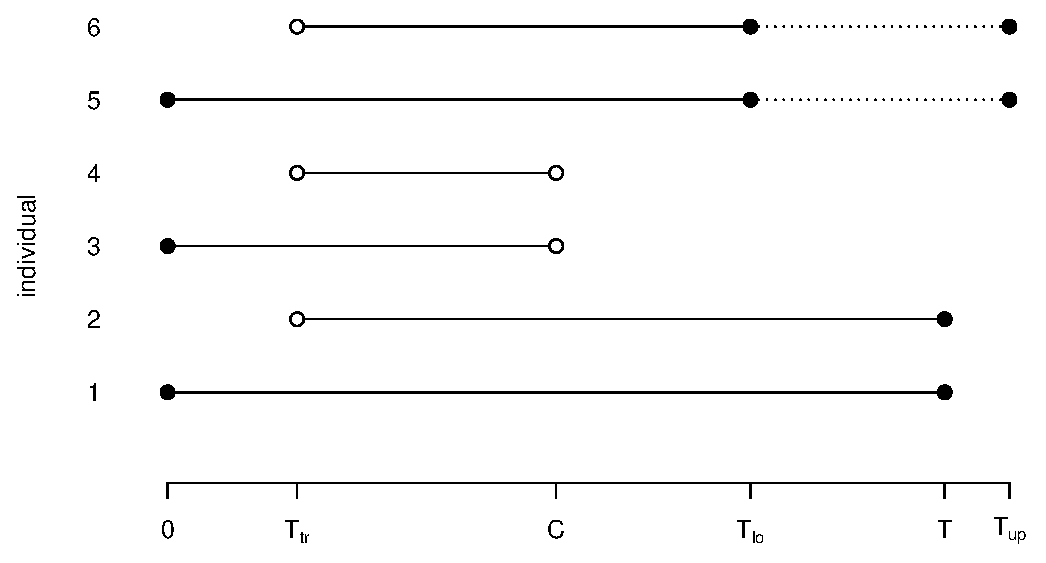
\epsfig{file=grafiken/censoringschemes.eps,scale=0.7}
{\it\caption{Illustration of different censoring
schemes.\label{censoringschemes}}}
\end{center}
\end{figure}

In a general framework an observation can now be uniquely described
 by the quadruple $(T_{tr},T_{lo},T_{up},\delta)$, with
\begin{center}
\begin{tabular}{ll}
$T_{lo}=T_{up}=T$, $\delta=1$ & if the observation is uncensored,\\
$T_{lo}=T_{up}=C$, $\delta=0$ & if the observation is right censored,\\
$T_{lo}<T_{up}$, $\delta=0$ & if the observation is interval censored.\\
\end{tabular}
\end{center}
For left truncated observations we have $T_{tr}>0$ while $T_{tr}=0$
for observations which are not truncated.

Based on these definitions we can now construct the likelihood
contributions for the different censoring schemes in terms of the
hazard rate $\lambda(t)$ and the survivor function
$S(t)=\exp(\int_0^t\lambda(u)du)$. Under the common assumption of
noninformative censoring and conditional independence, the
likelihood is given by
\begin{equation}\label{likelihood}
 L=\prod_{i=1}^n L_i,
\end{equation}
where
\[L_i = \lambda(T_{up})S(T_{up})/S(T_{tr}) = \lambda(T_{up})\exp\left(-\int_{T_{tr}}^{T_{up}}\lambda(t)dt\right)\]
for an uncensored observation,
\[L_i = S(T_{up})/S(T_{tr}) = \exp\left(-\int_{T_{tr}}^{T_{up}}\lambda(t)dt\right)\]
for a right censored observation and
\[L_i = (S(T_{lo})-S(T_{up}))/S(T_{tr}) = \exp\left(-\int_{T_{tr}}^{T_{lo}}\lambda(t)dt\right)\left(1-\exp\left(-\int_{T_{lo}}^{T_{up}}\lambda(t)dt\right)\right)\]
for an interval censored observation. Note that for explicit
evaluation of the likelihood (\ref{likelihood}) some numerical
integration technique has to be employed, since none of the
integrals can in general be solved analytically.

The above notation also allows for the easy inclusion of piecewise
constant, time-varying covariates via some data augmentation. Noting
that
\[\int_{T_{tr}}^{T}\lambda(t)dt = \int_{T_{tr}}^{t_1}\lambda(t)dt + \int_{t_1}^{t_2}\lambda(t)dt + \ldots + \int_{t_{p-1}}^{t_p}\lambda(t)dt + \int_{t_p}^{T}\lambda(t)dt\]
for $T_{tr}<t_1<\ldots<t_q<T$, we can replace an observation
$(T_{tr},T_{lo},T_{up},\delta)$ by a set of new observations
$(T_{tr},t_1,t_1,0)$, $(t_1,t_2,t_2,0)$, \ldots
$(t_{p-1},t_p,t_p,0)$, $(t_{p},T_{lo},T_{up},\delta)$ without
changing the likelihood. Therefore, observations with time-varying
covariates can be split up into several observations, where the
values $t_1<\ldots<t_p$ are defined by the changepoints of the
covariate and the covariate is now time-constant on each of the
intervals. In theory, other paths for a covariate $x(t)$ than
piecewise constant ones are also possible, if $x(t)$ is known for
$T_{tr}\le t\le T_{lo}$. In this case the the likelihood
(\ref{likelihood}) can also be evaluated numerically but a general
path $x(t)$ may lead to complicated data structures.

Figure \ref{timevaryingcovs} illustrates the data augmentation step
for a left truncated, uncensored observation and a covariate $x(t)$
that takes the three different values $x_1,x_2$ and $x_3$ on the
three intervals $[T_{tr},t_1], [t_1,t_2]$ and $[t_2,T_{up}]$. Here,
the original observation $(T_{tr},T_{up},T_{up},1)$ has to be
replaced by $(T_{tr},t_1,t_1,0)$, $(t_1,t_2,t_2,0)$ and
$(t_2,T_{up},T_{up},1)$.
\begin{figure}[htb]
\begin{center}
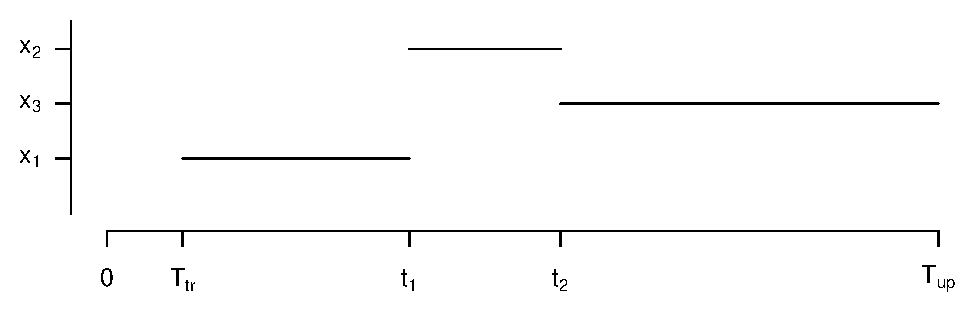
\epsfig{file=grafiken/timevaryingcovs.eps,scale=0.7}
{\it\caption{Illustration of time-varying
covariates.\label{timevaryingcovs}}}
\end{center}
\end{figure}

Currently, interval censored survival times can only be handled with
{\em remlreg objects}.

\subsection{Continuous-time multi-state models}\label{msmodels}
\index{Multi-state models}\index{Recurrent Events}\index{Disease
progression}\index{Competing risks}

Multi-state models are a flexible tool for the analysis of
time-continuous phenomena that can be characterized by a discrete
set of states. Such data structures naturally arise when observing a
discrete response variable for several individuals or objects over
time. Some common examples are depicted in Figure~\ref{some_msms} in
terms of their reachability graph for illustration. For recurrent
events (Figure~\ref{some_msms} (a)), the observations evolve through
time moving repeatedly between a fixed set of states. Other model
classes involve absorbing states, for example disease progression
models (Figure~\ref{some_msms} (b)), that are used to describe the
chronological development of a certain disease. If the severity of
this disease can be grouped into $q-1$ ordered stages of increasing
severity, a reasonable model might look like this: Starting from
disease state '$j$', an individual can only move to contiguous
states, i.e. either the disease gets worse and the individual moves
to state '$j+1$', or the disease attenuates and the individual moves
to state '$j-1$'. In addition, death is included as a further,
absorbing state '$q$', which can be reached from any of the disease
states. A model with several absorbing states is the competing risks
model (Figure~\ref{some_msms} (c)) where, for example, different
causes of death are analysed simultaneously.

\begin{figure}
\begin{center}
 \input{grafiken/msm_examples.tex}
 \caption{Reachability graphs of some common multi-state
 models.\label{some_msms}}
\end{center}
\end{figure}

A multi-state model is fully described by a set of hazard rates
$\lambda_{hi}(t)$ where $h$, $h=1,\ldots,k$, indexes the type of the
transition and $i$, $i=1,\ldots,n$, indexes the individuals. Since
the hazard rates describe durations between transitions, we specify
them in analogy to hazard rate models for continuous time survival
analysis. To be more specific, $\lambda_{hi}(t)$ is modelled in a
multiplicative Cox-type way as
\[
 \lambda_{hi}(t) = \exp(\eta_{hi}(t)),
\]
where
\begin{equation}\label{addpred}
 \eta_{hi}(t) = g_{h0}(t) + \sum_{l=1}^Lg_{hl}(t)u_{il}(t) +
 \sum_{j=1}^Jf_{hj}(x_{ij}(t)) + v_i(t)'\gamma_h +  b_{hi}
\end{equation}
is an additive predictor consisting of the following components:
\begin{itemize}
 \item A time-varying, nonparametric baseline effect $g_{h0}(t)$ common for all
 observations.
 \item Covariates $u_{il}(t)$ with time-varying effects $g_{hl}(t)$.
 \item Nonparametric effects $f_{hj}(x_{ij}(t))$ of continuous covariates
 $x_{ij}(t)$.
 \item Parametric effects $\gamma_h$ of covariates $v_i(t)$.
 \item Frailty terms $b_{hi}$ to account for unobserved
 heterogeneity.
\end{itemize}

For each individual $i$, $i=1,\ldots,n,$ the likelihood contribution
in a multi-state model can be derived from a counting process
representation of the multi-state model. Let $N_{hi}(t)$,
$h=1,\ldots,k$ be a set of counting processes counting transitions
of type $h$ for individual $i$. Consequently, $h=1,\ldots,k$ indexes
the observable transitions in the model under consideration and the
jumps of the counting processes $N_{hi}(t)$ are defined by the
transition times of the corresponding multi-state process for
individual $i$.

From classical counting process theory (see e.g. \citeasnoun{Andetal93}, Ch.~VII.2), the intensity processes $\alpha_{hi}(t)$
of the counting processes $N_{hi}(t)$ are defined as the product of the hazard rate for type $h$ transitions $ \lambda_{hi}(t)$
and a predictable at-risk indicator process $Y_{hi}(t)$, i.e.
\[
 \alpha_{hi}(t) = Y_{hi}(t) \lambda_{hi}(t),
\]
where the hazard rates are constructed in terms of covariates as in
(\ref{addpred}). The at-risk indicator $Y_{hi}(t)$ takes the value
one if individual $i$ is at risk for a type $h$ transition at time
$t$ and zero otherwise. For example, in the multi-state model of
Figure~\ref{some_msms}a), an individual in state 2 is at risk for
both transitions to state 1 and state 3. Hence, the at-risk
indicators for both the transitions '2 to 1' and '2 to 3' will be
equal to one as long as the individual remains in state 2.

Under mild regularity conditions, the individual log-likelihood
contributions can now be obtained from counting process theory as
\begin{equation}\label{loglike1}
 l_i = \sum_{h=1}^k\left[ \int_0^{T_i}\log(\lambda_{hi}(t))dN_{hi}(t) -
 \int_0^{T_i}\lambda_{hi}(t)Y_{hi}(t)dt\right],
\end{equation}
where $T_i$ denotes the time until which individual $i$ has been
observed. The likelihood contributions can be interpreted similarly
as with hazard rate models for survival times (and in fact coincide
with these in the case of a multi-state process with only one
transition to an absorbing state). The first term corresponds to
contributions at the transition times since the integral with
respect to the counting process in fact equals a simple sum over the
transition times. Each of the summands is then given by the
log-intensity for the observed transition evaluated at this
particular time point. In survival models this term simply equals
the log-hazard evaluated at the survival time for uncensored
observations. The second term reflects cumulative intensities
integrated over accordant waiting periods between two successive
transitions. The integral is evaluated for all transitions the
corresponding person is at risk at during the current period. In
survival models there is only one such transition (the transition
from 'alive' to 'dead') and the integral is evaluated from the time
of entrance to the study to the survival or censoring time.

More details on multi-state models, including an exemplary analysis on human sleep, can be found in \citeasnoun{KneHen06}.

\addcontentsline{toc}{section}{Bibliography}

\begin{thebibliography}{99}

\harvarditem{Albert \& Chib}{1993}{AlbChi93}
 {\scshape Albert, J. \& Chib, S.} (1993).
 Bayesian analysis of binary and polychotomous response data.
 {\it Journal of the American Statistical Association}, {\bf 88}, 669--679.

\harvarditem{Andersen et al.}{1993}{Andetal93}
 {\scshape Andersen, P. K., Borgan, {\O}, Gill, R. D. \& Keiding, N.} (1993).
 {\it Statistical Models Based on Counting Processes.}
 New York: Springer Verlag.

\harvarditem{Andrews \& Mallows}{1974}{AndMal74}
 {\scshape Andrews, D. F. \& Mallows, C. L.} (1974).
 Scale mixtures of normal distributions.
 {\it Journal of the Royal Statistical Society B}, {\bf 36}, 99--102.

\harvarditem{Bollaerts, Eilers \& van Mechelen}{2006}{BolEilvMe06}
 {\scshape Albert, J. \& Chib, S.} (1993).
 Simple and Multiple P-Spline Regression with Shape Constraints.
 {\it British Journal of Mathematical and Statistical Psychology}, {\bf 59}, 451--469.

\harvarditem{Belitz}{2007}{Bel07}
 {\scshape Belitz, C.} (2007).
 {\it Model Selection in Generalized Structured Additive Regression Models.}
 PhD Thesis, University of Munich.

\harvarditem{Belitz \& Lang}{2008}{BelLan08}
{\scshape Belitz, C. \& Lang, S.} (2008).
 Simultaneous selection of variables and smoothing parameters in structured additive regression models.
{\it Computational Statistics and Data Analysis}, {\bf 53} , 61-81.

\harvarditem{Besag, York \& Molli\'{e}}{1991}{BesYorMol91}
 {\scshape Besag, J., York, J. \& Molli\'{e}, A.} (1991).
 Bayesian image restoration with two applications in spatial statistics (with discussion).
 {\it Annals of the Institute of Statistical Mathematics}, {\bf 43}, 1--59.

\harvarditem{Brezger \& Lang}{2006}{BreLan06}
 {\scshape Brezger, A. \& Lang, S.} (2006).
 Generalized additive regression based on Bayesian P-splines.
 {\it Computational Statistics and Data Analysis} {\bf 50}, 967--991.

\harvarditem{Devroye}{1986}{Dev86}
 {\scshape Devroye, L.} (1986).
 {\it Non-Uniform Random Variate Generation.}
 New York: Springer Verlag.

\harvarditem{Eilers \& Marx}{1996}{EilMar96}
 {\scshape Eilers, P. H. C. \& Marx, B. D.} (1996).
 Flexible smoothing using B-splines and penalized likelihood (with comments and rejoinder).
 {\it Statistical Science}, {\bf 11}, 89--121.

\harvarditem{Fahrmeir, Kneib \& Lang}{2004}{FahKneLan04}
 {\scshape Fahrmeir, L., Kneib, T. \& Lang, S.} (2004).
 Penalized structured additive regression for space-time data: A Bayesian perspective.
 {\it Statistica Sinica}, {\bf 14}, 715--745.

\harvarditem{Fahrmeir \& Lang}{2001}{FahLan01a}
 {\scshape Fahrmeir, L. \& Lang, S.} (2001a).
 Bayesian Inference for Generalized Additive Mixed Models Based on Markov Random Field Priors.
 {\it Journal of the Royal Statistical Society C}, {\bf 50}, 201--220.

\harvarditem{Fahrmeir \& Lang}{2001}{FahLan01b}
 {\scshape Fahrmeir, L. \& Lang, S.} (2001b).
 Bayesian Semiparametric Regression Analysis of Multicategorical Time-Space Data.
 {\it Annals of the Institute of Statistical Mathematics}, {\bf 53}, 10--30.

\harvarditem{Fahrmeir \& Osuna}{2006}{FahOsu06}
 {\scshape Fahrmeir, L. \& Osuna, L.} (2006).
 Structured additive regression for overdispersed and zero-inflated count data.
 {\it Applied Stochastic Models in Business and Industry}, {\bf 22}, 351--369

 \harvarditem{Fahrmeir \& Tutz}{2001}{FahTut01}
 {\scshape Fahrmeir, L. \& Tutz, G.} (2001).
 {\it Multivariate Statistical Modelling based on Generalized Linear Models.}
 New York: Springer-Verlag.

\harvarditem{Fotheringham, Brunsdon \& Charlton}{2002}{FotBruCha02}
 {\scshape Fotheringham, A. S., Brunsdon, C., \& Charlton, M. E.} (2002).
 {\it Geographically Weighted Regression: The Analysis of Spatially Varying Relationships.}
 Chichester: Wiley.

\harvarditem{Gamerman}{1997}{Gam97}
 {\scshape Gamerman, D.} (1997).
 Efficient Sampling from the posterior distribution in generalized linear models.
 {\it Statistics and Computing}, {\bf 7}, 57--68.

\harvarditem{Gelfand, Sahu \& Carlin}{1996}{GelSahCar96}
 {\scshape Gelfand, A. E., Sahu, S. K. \& Carlin, B. P.} (1996).
 Efficient Parametrizations for Genera\-lized Linear Mixed Models.
 In: Bernardo, J. M., Berger, J. O., Dawid, A. P. \& Smith, A. F. M. (eds.),
 {\it Bayesian Statistics 5}, 165--180.
 Oxford University Press.

\harvarditem{George \& Liu}{1981}{GeoLiu81}
 {\scshape George, A. \& Liu, J.W.} (1981).
 {\it Computer Solution of Large Sparse Positive Definite Systems.}
 Series in computational mathematics, Prentice-Hall.

\harvarditem{Green}{1987}{Gre87}
 {\scshape Green, P. J.} (1987).
 Penalized likelihood for general semiparametric regression models.
 {\it International Statistical Review}, {\bf 55}, 245--259.

\harvarditem{Green}{2001}{Gre01}
 {\scshape Green, P. J.} (2001).
 A Primer in Markov Chain Monte Carlo.
 In: Barndorff-Nielsen, O. E., Cox, D. R. \& Kl\"{u}ppelberg, C. (eds.),
 {\it Complex Stochastic Systems}, 1--62.
 Chapmann and Hall, London.

\harvarditem{Green \& Silverman}{1994}{GreSil94}
 {\scshape Green, P. J. \& Silverman, B.} (1994).
 {\it Nonparametric Regression and Generalized Linear Models.}
 Chapman and Hall, London.

\harvarditem{Griffin \& Brown}{2005}{GriBro05}
 {\scshape Griffin, J. E., and Brown, P. J.} (2005). Alternative prior distributions
 for variable selection with very many more variables than observations. Technical
 report, University of Warwick, Dept. of Statistics.

\harvarditem{Harville}{1977}{Har77}
 {\scshape Harville, D. A.} (1977).
 Maximum Likelihood approaches to variance component estimation and to related problems.
 {\it Journal of the American Statistical Association}, {\bf 72}, 320--338.

\harvarditem{Hastie \& Tibshirani}{1990}{HasTib90}
 {\scshape Hastie, T. \& Tibshirani, R.} (1990).
 {\it Generalized additive models.}
 Chapman and Hall, London.

\harvarditem{Hastie \& Tibshirani}{1993}{HasTib93}
 {\scshape Hastie, T. \& Tibshirani, R.} (1993).
 Varying-coefficient Models.
 {\it Journal of the Royal Statistical Society B}, {\bf 55}, 757--796.

\harvarditem{Hastie \& Tibshirani}{2000}{HasTib00}
 {\scshape Hastie, T. \& Tibshirani, R.} (2000).
 Bayesian Backfitting.
 {\it Statistical Science}, {\bf 15}, 193--223.

\harvarditem{Hastie, Tibshirani \& Firedman}{2001}{HasTibFri01}
 {\scshape Hastie, T., Tisbshirani, R. \& Friedman, J.} (2001).
 {\it The Elements of Statistical Learning: Data Mining, Inference and Prediction.}
 New York: Springer-Verlag.

\harvarditem{Hennerfeind, Brezger \& Fahrmeir}{2006}{HenBreFah06}
 {\scshape Hennerfeind, A., Brezger, A. \& Fahrmeir, L.} (2006).
 Geoadditive survival models.
 {\it Journal of the American Statistical Association}, {\bf 101}, 1065--1075.

\harvarditem{Holmes \& Held}{2006}{HolHel06}
 {\scshape Holmes, C., Held, L.} (2006).
 Bayesian auxiliary variable models for binary and multinomial regression.
 {\it Bayesian Analysis}, {\bf 1}, 145--168.

\harvarditem{Hurvich, Simonoff \& Tsai}{1998}{HurSimTsa98}
 {\scshape Hurvich, C. M., Simonoff, J. S. \& Tsai, C. L.} (1998).
 Smoothing parameter selection in nonparametric regression using an improved {A}kaike information criterion.
 {\it Journal of the Royal Statistical Society B}, {\bf 60}, 271--293.

\harvarditem{Ishwaran \& Rao}{2005}{IshRao05}
 {\scshape Ishwaran, H., and Rao, S. J.} (2005). Spike and Slab Variable
 Selection: Frequentist and Bayesian Strategies. {\it The Annals of Statistics},
 {\bf 33}, 730-773.

\harvarditem{Johnson, Moore \& Ylvisaker}{1990}{JohMooYlv90}
 {\scshape Johnson, M.E., Moore, L.M. \& Ylvisaker, D.} (1990).
 Minimax and maximin designs.
 {\it Journal of Statistical Planning and Inference}, {\bf 26}, 131--148.

\harvarditem{Kammann \& Wand}{2003}{KamWan03}
 {\scshape Kammann, E. E. \& Wand, M. P.} (2003).
 Geoadditive Models.
 {\it Journal of the Royal Statistical Society C}, {\bf 52}, 1--18.

\harvarditem{Kneib}{2006}{Kne06}
 {\scshape Kneib, T.} (2006).
 Geoadditive hazard regression for interval censored survival times.
 {\it Computational Statistics and Data Analysis}, {\bf 51}, 777--792

\harvarditem{Kneib \& Hennerfeind}{2006}{KneHen06}
 {\scshape Kneib, T. \& Hennerfeind, A.} (2006).
 Bayesian Semiparametric Multi-State Models.
 {\it Statistical Modelling}, {\bf 8}, 169--198.

\harvarditem{Kneib \& Fahrmeir}{2006}{KneFah06}
 {\scshape Kneib, T. \& Fahrmeir, L.} (2006).
 Structured additive regression for categorical space-time data: A mixed model approach.
 {\it Biometrics}, {\bf 62}, 109--118.

\harvarditem{Kneib \& Fahrmeir}{2007}{KneFah07}
 {\scshape Kneib, T. \& Fahrmeir, L.} (2007).
 A mixed model approach to structured hazard regression.
 {\it Scandinavian Journal of Statistics}, {\bf 34}, 207--228.

\harvarditem{Kneib et al.}{2009}{Kne09}
 {\scshape Kneib, T., Konrath, S. und Fahrmeir, L.} (2009). High-dimensional
 Structured Additive Regression Models: Bayesian Regularisation, Smoothing and Predictive
 Performance. Department of Statistics, Technical Report No. 46, LMU Munich.

\harvarditem{Knorr-Held}{1999}{KnoHel99}
 {\scshape Knorr-Held, L.} (1999).
 Conditional Prior Proposals in Dynamic Models.
 {\it Scandinavian Journal of Statistics}, {\bf 26}, 129--144.

\harvarditem{Konrath et al.}{2008}{Kon08}
 {\scshape Konrath, S., Kneib, T., Fahrmeir, L.} (2008). Bayesian Regularisation
 in Structured Additive Regression Models for Survival Data. Department of Statistics,
 Technical Report No.35, LMU Munich.

\harvarditem{Lang \& Brezger}{2004}{LanBre04}
 {\scshape Lang, S. \& Brezger, A.} (2004).
 Bayesian P-splines.
 {\it Journal of Computational and Graphical Statistics}, {\bf 13}, 183--212.

\harvarditem{Lin \& Zhang}{1999}{LinZha99}
 {\scshape Lin, X. \& Zhang, D.} (1999).
 Inference in generalized additive mixed models by using smoothing splines.
 {\it Journal of the Royal Statistical Society B}, {\bf 61}, 381--400.

\harvarditem{McCullagh \& Nelder}{1989}{McCNel89}
 {\scshape McCullagh, P. \& Nelder, J. A.} (1989).
 {\it Generalized Linear Models.}
 Chapman and Hall, London.

\harvarditem{M\"{u}ller, Stadtm\"{u}ller \& Tabnak}{1997}{MueStaTab97}
 {\scshape M\"{u}ller, H. G., Stadtm\"{u}ller, U. \& Tabnak, F.} (1997).
 Spatial Smoothing of Geographically Aggregated Data, with Applications to the Construction of Incidence Maps.
 {\it Journal of the American Statistical Association} {\bf 92}, 61--71.

\harvarditem{Nychka \& Saltzman}{1998}{NycSal98}
 {\scshape Nychka, D. \& Saltzman, N.} (1998).
 {\it Design of Air-Quality Monitoring Networks.}
 Lecture Notes in Statistics, 132, 51--76.

\harvarditem{Osuna}{2004}{Osu04}
 {\scshape Osuna, L.} (2004)
 {\it Semiparametric Bayesian Count Data Models}.
 Dr. Hut Verlag, M\"{u}nchen.

\harvarditem{Park \& Casella}{2008}{ParCas08}
 {\scshape Park, T., and Casella, G.} (2008). The Bayesian Lasso.
 {\it Journal of the American Statistical Association}, {\bf 482}, 681-686.

\harvarditem{Rue}{2001}{Rue01}
 {\scshape Rue, H.} (2001).
 Fast Sampling of Gaussian Markov Random Fields with Applications.
 {\it Journal of the Royal Statistical Society B}, {\bf 63}, 325--338.

\harvarditem{Ruppert, Wand \& Carroll}{2003}{RupWanCar03}
 {\scshape Ruppert, D., Wand, M. P. \& Carroll, R. J.} (2003).
 {\it Semiparametric Regression.}
 Cambridge University Press.

\harvarditem{Spiegelhalter et al.}{2002}{SpiBesCar02}
 {\scshape Spiegelhalter, D. J., Best, N. G., Carlin, B. P. \& van der Linde, A.} (2002).
 Bayesian measures of model complexity and fit.
 {\it Journal of the Royal Statistical Society B}, {\bf 65}, 583--639.

\end{thebibliography}

\addcontentsline{toc}{section}{Index}
\input{manual_star.ind}
\hypertarget{index}{}

\end{document}

\hypertarget{index}{}

\end{document}

\hypertarget{index}{}

\end{document}

\hypertarget{index}{}

\end{document}
